\documentclass[a4paper,
11pt,
BCOR=7mm,
onecolumn,
headsepline,
captions=tableheading,
parskip=half,
ngerman,
bibtotocnumbered,
listof=totoc]{scrartcl}
%Allgemein:
\usepackage[T1]{fontenc}
\usepackage[utf8]{inputenc}
\usepackage[ngerman]{babel}
\usepackage[autooneside=false,automark]{scrlayer-scrpage}
%Schriftart:
\usepackage{lmodern}
%mal schauen:
\usepackage[font=small,labelfont=it]{caption}
\usepackage{here}

\usepackage[onehalfspacing]{setspace} %Für richtigen Abstand der Absätze
%Für Chemie:
\usepackage{chemmacros}
\usepackage{chemformula}
\usepackage{ghsystem}
\usepackage{chemfig}
\usepackage{siunitx}
%Für Tabellen
\usepackage{tabularx}
\usepackage{multicol}
\usepackage{longtable}
\usepackage{booktabs} 	%\*rule-Befehle
\usepackage{array}		%p und b Spalten
%Grafiken
\usepackage{graphicx}
\usepackage{subfig}
%Literatur/Zitieren
\usepackage[autostyle, german=quotes]{csquotes}
\usepackage[sorting=none,doi=false,url=false,autocite=superscript,sortcites=true, labelnumber=true]{biblatex}
%Mehr Zeichen:
\usepackage{amsmath}
\usepackage{amssymb}
%Fußnoten:
\usepackage{savefnmark}
%Aufzählungen
\usepackage{mdwlist}
\usepackage{paralist}
\usepackage{enumerate}
%Für Verweise:
\usepackage{varioref}
\usepackage{hyperref}
\usepackage{cleveref}
%
\usepackage{microtype}
\usepackage{todonotes}

%Literaturdatei:
\bibliography{Literatur}

%Chemfig:
\renewcommand*\printatom[1]{\ensuremath{\mathsf{#1}}}
%SI soll , statt . als Trennzeichen
\sisetup{
output-decimal-marker = {,},
per-mode = symbol,
}
%Absatzabstand
\newcommand{\sref}[1]{(siehe \cref{#1})}

%Allgemeine Einstellungen:
\pagestyle{scrheadings}

%Silbentrennung:
\hyphenation{}

\begin{document}
%% !TEX root = BIGALL-Master.tex

\begin{titlepage}
\centering
\begin{figure}
	\centering

\includegraphics[width=0.3\linewidth,trim=0 0 0 5]{Bilder/LUH}
\end{figure}

\vspace{1cm}
%{\scshape\LARGE Leibniz Universität Hannover \par}
%\vspace{0.5cm}
%{\scshape\Large Masterarbeit\par}
%\vspace{1.5cm}
\noindent\hrule
{\huge\bfseries Synthese und Charakterisierung von nanopartikelbasierten Netzwerkstrukturen \par}
\noindent\hrule
\vspace{1cm}
{\scshape\Large Masterarbeit\par}
am Institut für Physikalische Chemie und Elektrochemie\\
der Leibniz Universität Hannover\\
Laboratorium für Nano- und Quantenengineering\\
\vspace{0.5cm}
im Studiengang Material- und Nanochemie\\
\vspace{0.5cm}
Zur Erlangung des akademischen Grades\\
Master of Science

\vfill
\begin{flushleft}
\begin{tabbing}
Autor: \qquad\qquad\qquad\qquad \= Björn Gastmann\\
Matrikelnummer: \> 10004554\\
Erstprüferin: \> Prof. Dr. Nadja Bigall\\
Zweitprüfer: \> Prof. Dr. Peter Behrens\\
Bearbeitungszeitraum: \> 31. September 2019 -- \today\\
Abgabe: \> \today\\
\end{tabbing}
\end{flushleft}
\end{titlepage}
% !TEX root = BIGALL-Master.tex

\begin{titlepage}
\centering
\begin{figure}
	\centering

\includegraphics[width=0.3\linewidth,trim=0 0 0 5]{Bilder/LUH}
\end{figure}

\vspace{1cm}
%{\scshape\LARGE Leibniz Universität Hannover \par}
%\vspace{0.5cm}
%{\scshape\Large Masterarbeit\par}
%\vspace{1.5cm}
\noindent\hrule
{\huge\bfseries Synthese und Charakterisierung von nanopartikelbasierten Netzwerkstrukturen \par}
\noindent\hrule
\vspace{1cm}
{\scshape\Large Masterarbeit\par}
am Institut für Physikalische Chemie und Elektrochemie\\
der Leibniz Universität Hannover\\
Laboratorium für Nano- und Quantenengineering\\
\vspace{0.5cm}
im Studiengang Material- und Nanochemie\\
\vspace{0.5cm}
Zur Erlangung des akademischen Grades\\
Master of Science

\vfill
\begin{flushleft}
\begin{tabbing}
Autor: \qquad\qquad\qquad\qquad \= Björn Gastmann\\
Matrikelnummer: \> 10004554\\
Erstprüferin: \> Prof. Dr. Nadja Bigall\\
Zweitprüfer: \> Prof. Dr. Peter Behrens\\
Bearbeitungszeitraum: \> 31. September 2019 -- \today\\
Abgabe: \> \today\\
\end{tabbing}
\end{flushleft}
\end{titlepage}
%
\tableofcontents
\pagebreak

% !TEX root = BIGALL-Master.tex
\section{Einleitung}
Nanopartikel sind für viele technische Anwendungen, wie z.B. in Photovoltaikanlagen, Photodetektoren und als Katalysatoren aufgrund ihrer einzigartigen optoelektronischen Eigenschaften und hohen Oberflächen-zu-Massen-Verhältnissen interessant. 
\autocite{Afzaal2006,Cai2006,Law2005,Yan2003}
Ein Problem dieser Nanopartikel ist es, dass für diese Anwendungen meist keine kolloidalen Lösungen benötigt werden, sondern Nanopartikelanordnungen im festen Zustand.
Aus diesem Grund wurden Nanopartikel zu Gelen formiert, da diese immernoch eine sehr hohes Oberflächen-zu-Massen-Verhältnis besitzen, dabei aber als fester Körper vorliegen.

Synthesen und Eigenschaften von Gelen aus Halbleiter- oder Metallnanopartikeln sind inzwischen sehr gut erforscht.\todo{Quellen}
Ebenso sind inzwischen auch Nanopartikel mit Heterostrukturen aus Metall und Halbleiter gut untersucht.
Was bisher allerdings in der Forschung vernachlässigt wurde, sind Gele mit Heterostrukturen aus Halbleiter- und Metallnanopartikeln.
Und diese sind bisher entweder Gele die aus heterostrukturierten Nanopartikeln gebaut werden,\autocite{Nahar2015,Lesnyak2011} oder Halbleitergele an die Metallnanopartikel gesetzt werden. \autocite{Gill2009,Gill2011}

In dieser Arbeit soll eine Methode entwickelt werden Metallnanopartikelgele mit Halbleiternanopartikel zu besetzen.
Da Gele sehr poröse Stoffe sind und auch in diesen Poren Halbleiternanopartikel herangewachsen werden sollen, muss ein Verfahren für die Synthese von Halbleitern verwendet werden bei denen die Edukte genug Zeit haben um in diese Poren einzudringen.
Gleichzeitig sind nicht zu hohe Temperaturen von Vorteil um die Stabilität der Gele nicht zu gefährden.
Aus diesem Grund werden in dieser Arbeit die Verwendung von Single-Source-Precursoren als Halbleiterquelle untersucht.
Diese bieten sich dadurch an, dass es zu keiner spontanen Reaktion der Edukte kommen kann, da nur die Single-Source-Precursor Lösung zugegeben wird, die ohne Temperaturzufuhr nicht reagiert, was dazu führt, dass der Lösung genug Zeit gelassen werden kann, um in die Poren zu gelangen. 
Gleichzeitig findet die thermische Zersetzung bei unter \SI{300}{\degreeCelsius} statt, wodurch zum einen noch in klassischen Lösemitteln wie TOP gearbeitet werden kann und zum anderen die Stabilität der Gele nicht zu stark angegriffen wird.
\pagebreak
% !TEX root = Bigall.tex
\section{Theoretische Grundlagen}

\pagebreak
% !TEX root = Bigall.tex
\section{Analytische Methoden}


\pagebreak
% !TEX root = Bigall.tex
\section{Experimentelles}
	\subsection{Chemikalien}
		\todo{Hersteller}
		\todo{Deutscher Namen?}
		\begin{table}[H]
			\centering
			\caption{Liste aller Verwendeten Chemikalien}
			\label{tab:Chemikalien}
			\begin{tabular}{ll}
				\toprule
				Chemikalie & Hersteller \\
				\midrule
				Aceton&\\
				Methanol (99\%)&\\
				Ethanol&\\
				trockenes Ethanol&\\
				Chloroform&\\
				Hydrogen tetrachloroaurate(III) ($\geq$99,9\%) & \\ 
				borane tert-butylamine(BBA, 97\%) &\\
				Tetralin (99\%)&\\
				Oleylamine ()&\\
				3-Mercaptopropionic acid (MPA,)&\\
				Kaliumhydroxid (KOH,99,9\%)&\\
				Silbernitrat&\\
				Natriumcitrat&\\
				Natriumborohydrid&\\
				Yttrium(III)chlorid Hexahydrat&\\
				Ytterbium(III)chlorid Hexahydrat&\\
				\bottomrule
			\end{tabular}
		\end{table}
	\subsection{Herstellung von Gelen}
		\subsubsection{Herstellung von Hydrogelen durch Yttrium und Ytterbium}
		\todo{Ref, Was wird geamcht?}
		
		
			\paragraph{Synthese von Gold-Nanopartikel in organischen Lösungsmitteln}
		
			\SI{200}{\milli\gram} Hydrogen tetrachloroaurate(III) werden gelöst in einer Lösung aus \SI{10}{\milli\liter} Tetralin und \SI{10}{\milli\liter} Oleylamine und in einem Eisbad für 20 Minuten gerührt.
			\SI{0,087}{\gram} BBA werden in \SI{1}{\milli\liter} Tetralin und \SI{1}{\milli\liter} Oleylamine gegeben und in einem Ultraschallbad gelöst und anschließend in gekühlte Lösung injiziert.
			Anschließen wird das Reaktionsgemisch für weitere \SI{2}{\hour} im Eisbad gerührt.
			Daraufhin wird die Lösung auf 2 \SI{50}{\milli\liter}-Zentrifugengefäße gleichmäßig aufgeteilt und zum Fällen der Partikel mit Aceton auf \SI{50}{\milli\liter} aufgefüllt und bei 8500~rpm für \SI{10}{\minute} zentrifugiert.
			Nach dem Zentrifugieren wurden die Partikel in \SI{3}{\milli\liter} je Zentrifugengefäß redispergiert.
			%Anschließend wurden die beiden Lösungen wieder zusammen in ein 25ml Schraubdeckelgläschen gegeben. Name: BG-AU-NP1. Verweis auf Liu2015
				
			\paragraph{Phasentransfer der Gold-Nanopartikel}
		
			Für den Phasentransfer werden je \SI{1}{\milli\liter} der Goldlösung in \SI{5}{\milli\liter} einer methanolischen \SI{0,1}{M}~KOH-Lösung gegeben und anschließend \SI{250}{\micro\liter} MPA dazugegeben und für \SI{4}{\hour} geschwenkt.
			Nach dem Abzentrifugieren (8500~rpm, 10 Minuten) wird der Rückstand in 4mL wässriger KOH-Lösung aufgenommen und dann \SI{1}{\milli\liter} Chloroform dazugegeben. 
			Da nach erneutem Zentrifugieren sich kein fester Rückstand gebildet hatte, wurden \SI{10}{\milli\liter} Aceton dazugegeben und das Zentrifugieren wiederholt.
				
			\paragraph{Gelierung der Gold-Nanopartikel mit Yttrium und Ytterbium}
				
			Es werden von den phasentransferierten Gold-Nanopartikeln, nach vorheriger Bestimmung der Goldkonzentration durch AAS-Messungen, Lösungen mit den Konzentrationen 0,625; 1,5 und \SI{2,5}{\gram\per\liter} hergestellt.
			Mit Yttrium(III)chlorid Hexahydrat bzw. Ytterbium(III)chlorid Hexahydrat werden je 3 Lösungen (1; 5; \SI{10}{mM}) hergestellt.
			Es werden immer \SI{200}{\micro\liter} Goldlösung und \SI{25}{\micro\liter} Yttrium- bzw. Ytterbium-Lösung dazugegeben zusammen in ein \SI{2}{\milli\liter}-Zentrifugengefäß gegeben und für \SI{24}{\hour} stehen gelassen.
			Dies wurde für jede Kombination aus Goldlösung und Y/Yb-Lösung, insgesammt 18, durchgeführt.
			Es bildet sich bei allen unten im Gefäß ein kleiner dunkler Klumpen.
			  
		\subsubsection{Herstellung von Hydrogelen durch Wasserstoffperoxid}
			Hier werden im ersten Schritt Gold- und Silbernanopartikel in wässriger Lösung synthetisiert und aufkonzentriert.
			Im zweiten Schritt wird dann die Gelierung ausgelöst. \autocite{Bigall2009} 
		 
			\paragraph{Synthese Goldnanopartikel in wässriger Phase mit Natriumcitrat}
			
			\SI{29}{\milli\liter} 0,2\%ige Goldchlorid-Lösung werden in \SI{500}{\milli\liter} dest. Wasser gegeben.
			Es werden \SI{11,6}{\milli\liter} einer 1\%igen Natriumcitratlösung dazugegeben und nach 30 Sekunden \SI{5,8}{\milli\liter}	einer eiskalten Lösung aus \SI{0,085}{\gram} Natriumborohydrid und \SI{0,5}{\gram} Natriumcitrat in \SI{50}{\milli\liter} dest. Wasser dazugegeben.
			Anschließend werden die Goldpartikel durch Zenrifugenfilter auf 10mL aufkonzentriert.
			
			\paragraph{Synthese Silbernanopartikel in wässriger Phase mit Natriumcitrat}
			
			\SI{12}{\milli\liter} 0,2\%ige Silbernitrat-Lösung werden in \SI{488}{\milli\liter} dest. Wasser gegeben und auf \SI{100}{\degreeCelsius} erhitzt.
			Anschließend werden \SI{11,6}{\milli\liter} einer 1\%igen Natriumcitratlösung dazugegeben.
			Nach 30 Sekunden werden  \SI{5,5}{\milli\liter}	einer eiskalten Lösung aus \SI{0,038}{\gram} Natriumborohydrid und \SI{0,5}{\gram} Natriumcitrat in \SI{50}{\milli\liter} dest. Wasser dazugegeben.
			Nach 2 Minuten wird alles im Dunkeln abgekühlt.
			Anschließend werden die Silberpartikel durch Zenrifugenfilter auf 10mL aufkonzentriert.
			
			\paragraph{Gelierungsprozess}
			    \begin{description}
			    \item[Gele aus Gold-Nanopartikeln:]
			    \SI{500}{\micro\liter} der Goldlösung werden in ein 2mL-Zentri"-fugen"-gefäß gegeben und anschließend \SI{40}{\micro\liter} einer 1\%igen Wasserstoffperoxid-Lösung gegeben und anschließend für X Tage dunkel gelagert.
			    \item[Gele aus Silber-Nanopartikeln:]
			    \SI{500}{\micro\liter} der Silberlösung werden in ein 2mL-Zentri"-fugen"-gefäß gegeben und anschließend \SI{200}{\micro\liter} einer 3\%igen Wasserstoffperoxid-Lösung gegeben und anschließend für X Tage dunkel gelagert.
			    \item[Bimetallisches Gel aus Gold/Silber-Nanopartikeln:]
			    \SI{500}{\micro\liter} der Goldlösung und 	\SI{500}{\micro\liter} der Silberlösung werden in ein 2mL-Zentri"-fugen"-gefäß gegeben und anschließend für X Tage dunkel gelagert.
			    \end{description}
			    
			
		\subsubsection{Ethanolischer Ansatz für direkte Synthese von Gelen}
			Im Gegensatz zu den vorherigen Ansätzen, sind hier Nanopartikelbildung und Gelierung keine zwei voneinander getrennte Syntheseschritte.
			Hier werden direkt aus der ethanolischen Metallsalzlösung die Gele gebildet. \autocite{Georgi2019}
			
			Unter Schutzatmosphäre werden \SI{39}{\milli\gram} Hydrogen tetrachloroaurate(III) in \SI{8}{\milli\liter} trockenem Ethanol gegeben.
			Eine zweite Lösung wird hergestellt aus \SI{11}{\milli\gram} NaBH$_4$ in \SI{6}{\milli\liter} trockenem Ethanol gegeben.
			Es werden 6 Proben präpariert, indem jeweils \SI{1,33}{\milli\liter} der Goldlösung in ein \SI{8}{\milli\liter}-Schraubdeckelglas gegeben wird und anschließend \SI{1}{\milli\liter} der zweiten Lösung dazugegeben wird.
			Die Lösung färbt sich sofort dunkel.
			Nach einer Stunde hat sich die Lösung klar gefärbt und es hatte sich entweder ein dunkel Bodensatz gebildet oder es schwamm ein Klumpen an der Oberfläche.
			Bei den Proben mit Bodensatz wurden die Gläser leicht schräg gehalten und gedreht, wodurch sich der Bodensatz zusammenklumpte und wie bei den anderen Proben, dieser Klumpen dann an der Oberfläche schwamm.  
			
	\subsection{Synthese von Kupfersulfid durch Single-Source-Precurser}
	    Für die Synthese von Kupfersulfid wird eine thermische Zersetzung eines Kupferkomplexes genutzt. \autocite{JenLaPlante2010}
		\subsubsection{Synthese des Single-Source-Precursors \ch{Cu[DDTC]2}}
	        Zur Herstellung des gewünschten Precursors (\ch{Cu[DDTC]2}) werden zwei Lösungen vorbereitet: 
    	    Einmal wurden \SI{0,2218}{\gram} \ch{CuCl2} in \SI{20}{\milli\liter} Wasser gelöst.
	        Für die zweite Lösung wurden \SI{0,7323}{\gram} \ch{Na[DDTC]* 3 H2O} in \SI{20}{\milli\liter} Wasser gelöst.
	        Anschließend werden beide Lösungen zusammengegeben, wobei sich direkt ein dunkler Niederschlag bildet.
	        Dieser wird abzentrifugiert und an Luft getrocknet.
	        Daraufhin wird es in heißem Chloroform rekristallisiert und erneut an Luft getrocknet.
		    Das entstandene \ch{Cu[DDTC]2} wird abgewogen und in TOP aufgenommen, sodass eine 0,11 molare Lösung erhalten wird.
		    
		\subsubsection{Herstellung Kupfersulfid}
		    Es werden \SI{100}{\micro\liter} der 0,11~M \ch{Cu[DDTC]2}-Lösung in ein \SI{8}{\milli\liter}-Schraubdeckelgläschen gegeben, dass in einem Sandbad auf \SI{290}{\degreeCelsius} unter Stickstoffatmosphäre erhitzt wird.
		    Dies wird solange erhitzt, bis das gesamte Lösemittel verdampft ist und ein schwarzer trockener Rückstand erkennbar ist.
		    Dieser wird in \SI{0,5}{\milli\liter} Toluol aufgenommen, anschließend \SI{1}{\milli\liter} Methanol dazugegeben und abzentrifugiert.
		    Der Rückstand wird in \SI{0,5}{\milli\liter} Toluol aufgenommen.
	
	\subsection{Synthese von CuS mit \ch{Cu[DDTC]2} und \ch{CuCl2}}
	    Da bekannt ist, dass Chloridionen einen starken Einfluss auf das Nukleationsverhalten bei Nanopartikeln haben kann\cite{Hinrichs2016}, wurde ein Teil des Single-Source-Precursors durch \ch{CuCl2} substituiert.
	    
	    
	\subsection{Synthese aus Goldnanopartikeln und Kupfer-diethyldithiocarbonat}
	
		Bei dieser Synthese wurde die CuS-Synthese, wie oben beschrieben, durchgeführt, mit einem Anteil an Gold-Nanopartikeln, mit der Absicht, dass die CuS-Bildung um die Nanopartikel herum stattfindet.	
	    Es werden \SI{100}{\micro\liter} der 0,11~M \ch{Cu[DDTC]2}-Lösung und verschiedene Mengen (\cref{tab:Au_Cu_Ratio} der Goldnanopartikel in Hexan in ein \SI{8}{\milli\liter}-Schraubdeckelgläschen zusammengegeben und in einem Sandbad unter Stickstoffatmosphäre auf \SI{290}{\degreeCelsius} erhitzt, bis das Lösemittel komplett verdampft ist.
	
    \begin{table}[H]
		\centering
		\caption{Die verschiedenen genutzten Verhältnisse aus Goldnanopartikeln und \ch{Cu[DDTC]2}.}
		\label{tab:Au_Cu_Ratio}
		\begin{tabular}{ll}
            \toprule
            V(Au)/\si{\micro\liter}&V(\ch{Cu[DDTC]2})/\si{\micro\liter}\\
            \midrule
            10&100\\
            20&100\\
            30&100\\
            40&100\\
            50&100\\
            100&100\\
            \bottomrule
        \end{tabular}
    \end{table}
	
\pagebreak
% !TEX root = BIGALL-Master.tex
\section{Messungen und Auswertung}

\subsection{Synthese Kupfersulfidnanopartikel}
	Bei dieser Synthese war das Ziel Kupfersulfid aus dem Single-Source-Precursor \ch{Cu[DDTC]2} als Nanopartikel herzustellen. 
	Die Partikel wurden per UV-vis-NIR-Spektroskopie und mit TEM untersucht.
	Das Absorptionsspektrum zeigt ein Maximum bei $\lambda_{max}$=\SI{330}{\nano\meter}, mit einer kleinen Schulter bei \SI{360}{\nano\meter}.
	Die TEM Bilder zeigen, dass die Nanopartikel eine hexagonale Form besitzen und etwa \SI{350}{\nano\meter} als Durchmesser besitzen.
	Die Partikel sind so erstmal viel größer, als später die Partikel und Gele um die sich die Schale bilden soll.
	Dies sollte allerdings kein Problem darstellen, da sobald diese Synthese in Anwesenheit von anderen Partikel stattfindet diese das Nukleationsverhalten beeinflussen können.
	
	
	\begin{figure}[H]
		\centering
		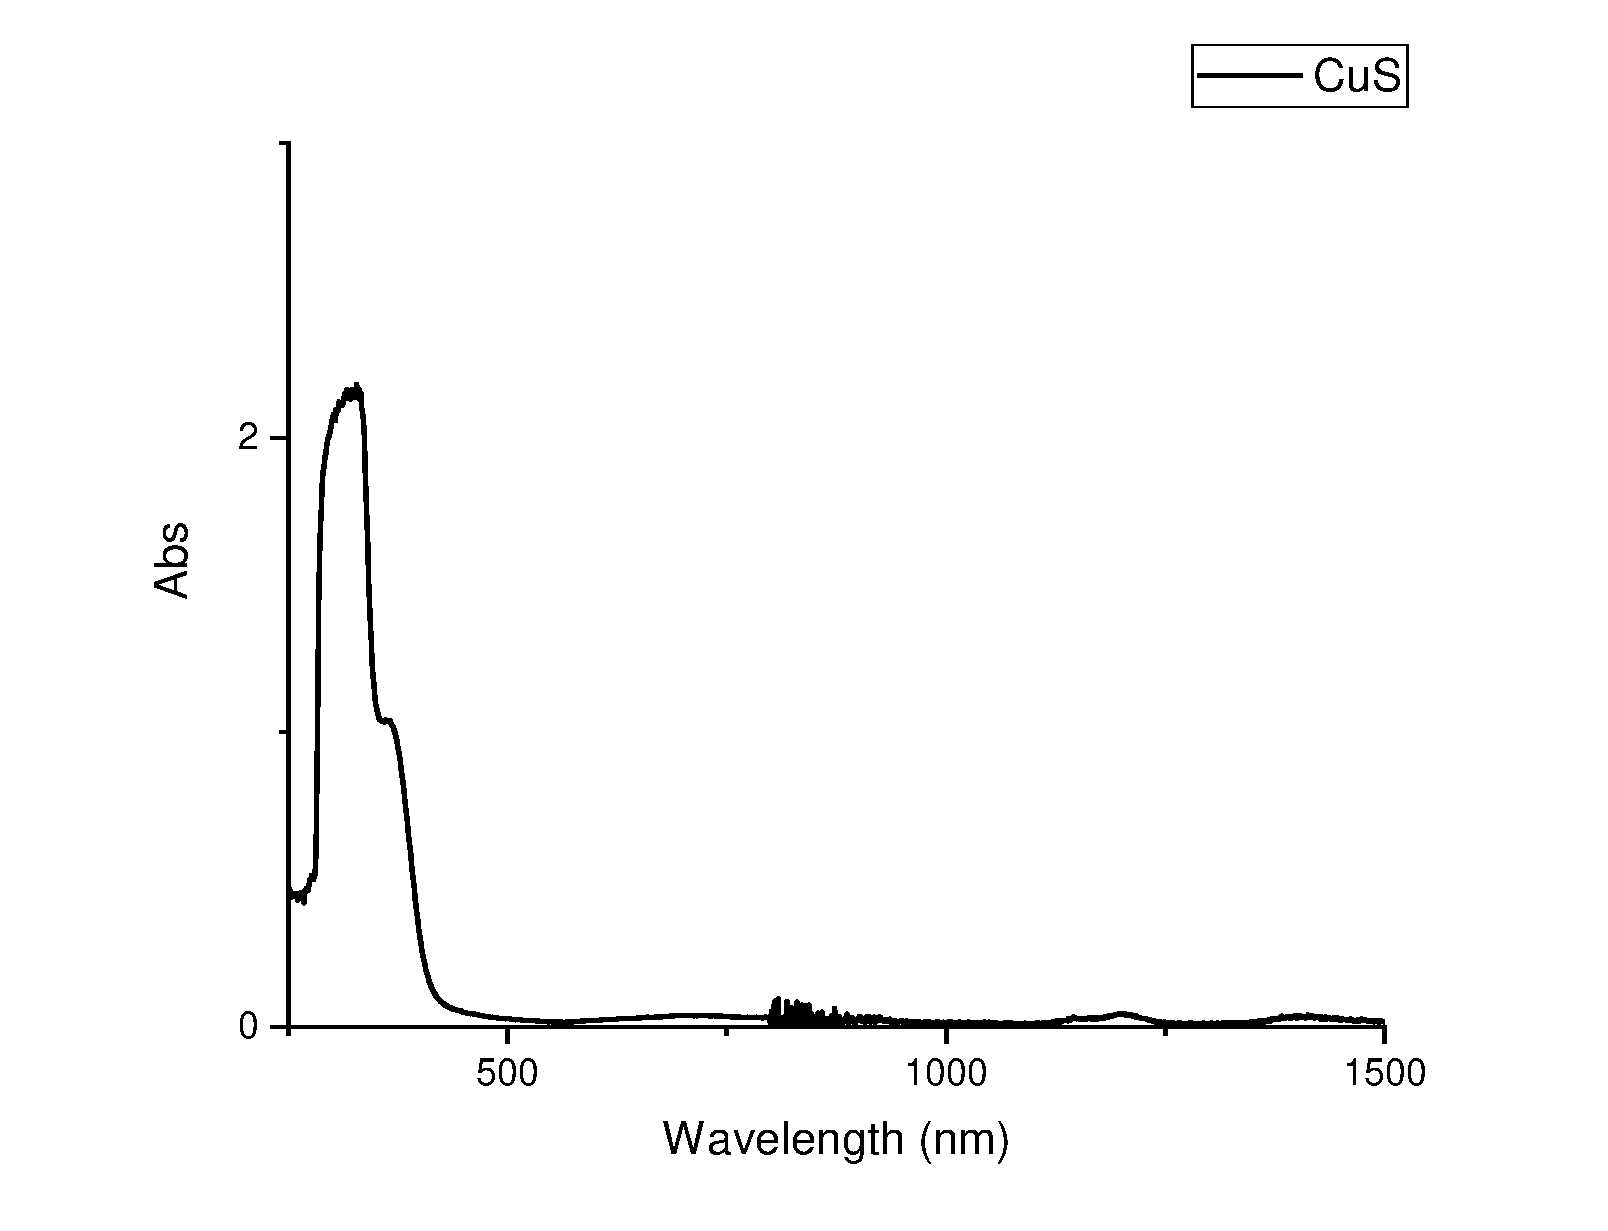
\includegraphics[width=0.6\textwidth]{Bilder/UV-CuS} 	
		\caption{Absorptionsspektrum der CuS-Nanopartikel in Toluol, gemessen in einer Ulbrichtkugel.}
		\label{fig:UV-CuS}
	\end{figure}
	
	\begin{figure}[H]
		\centering
		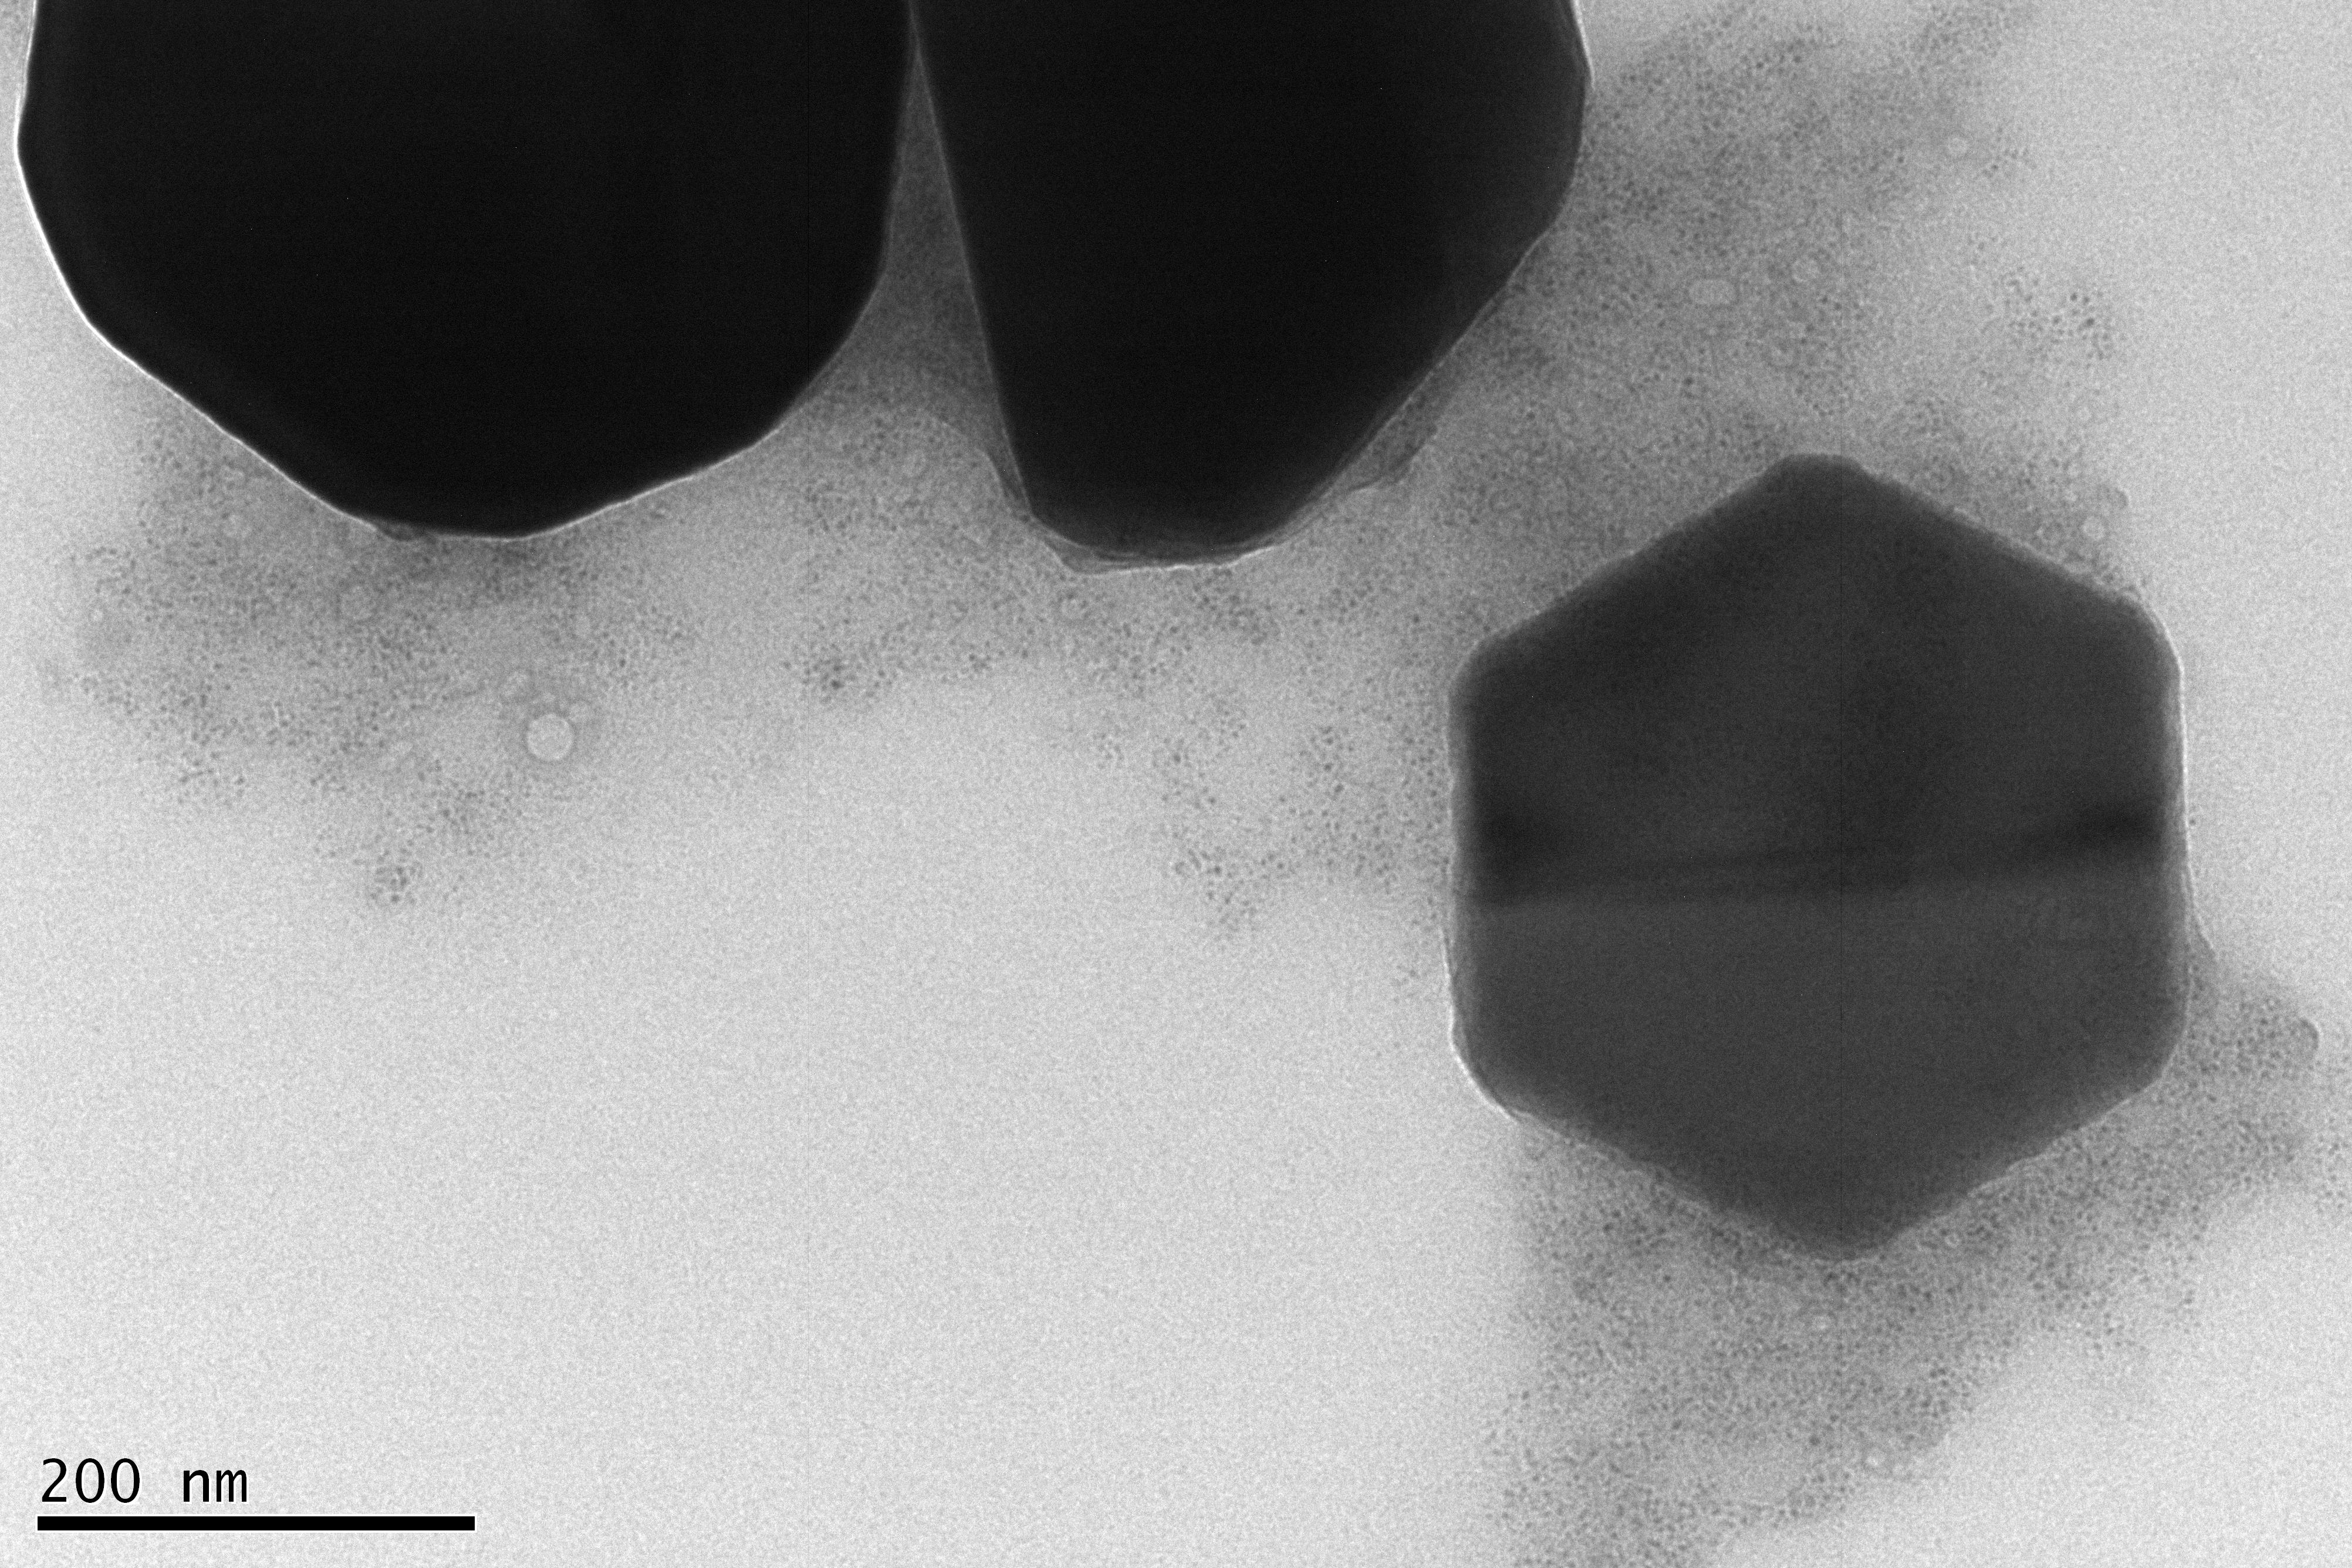
\includegraphics[width=0.6\textwidth]{Bilder/TEM-CuS} 	
		\caption{TEM-Bild der CuS-Nanopartikel.}
		\label{fig:TEM-CuS}
	\end{figure}
	
\subsection{Synthese Goldnanopartikel}
	Bei dieser Synthese war es das Ziel möglichst monodisperse Goldnanopartikel herzustellen.
	Die Partikel wurden per UV-vis-Spektroskopie und mit TEM untersucht.
	Das UV-vis zeigt ein für Gold typisches, durch LOPR bedingte, Absorptionsmaximum von $\lambda_{Gold}$=\SI{519}{\nano\meter}, wie in \cref{fig:UV-AuNP} dargestellt.
	Aus den TEM-Bildern geht hervor, dass die Partikel eine mittlere Größe von etwa \SI{7,6}{\nano\meter} mit einer Abweichung von etwa \SI{0,6}{\nano\meter}, wie \cref{fig:TEM-Au-Hex-2} zeigt.	
	Die Partikel zeigten also eine zufriedenstellende Größenverteilung und können somit für weitere Experimente verwendet werden.
	
	\begin{figure}[H]
		\centering
		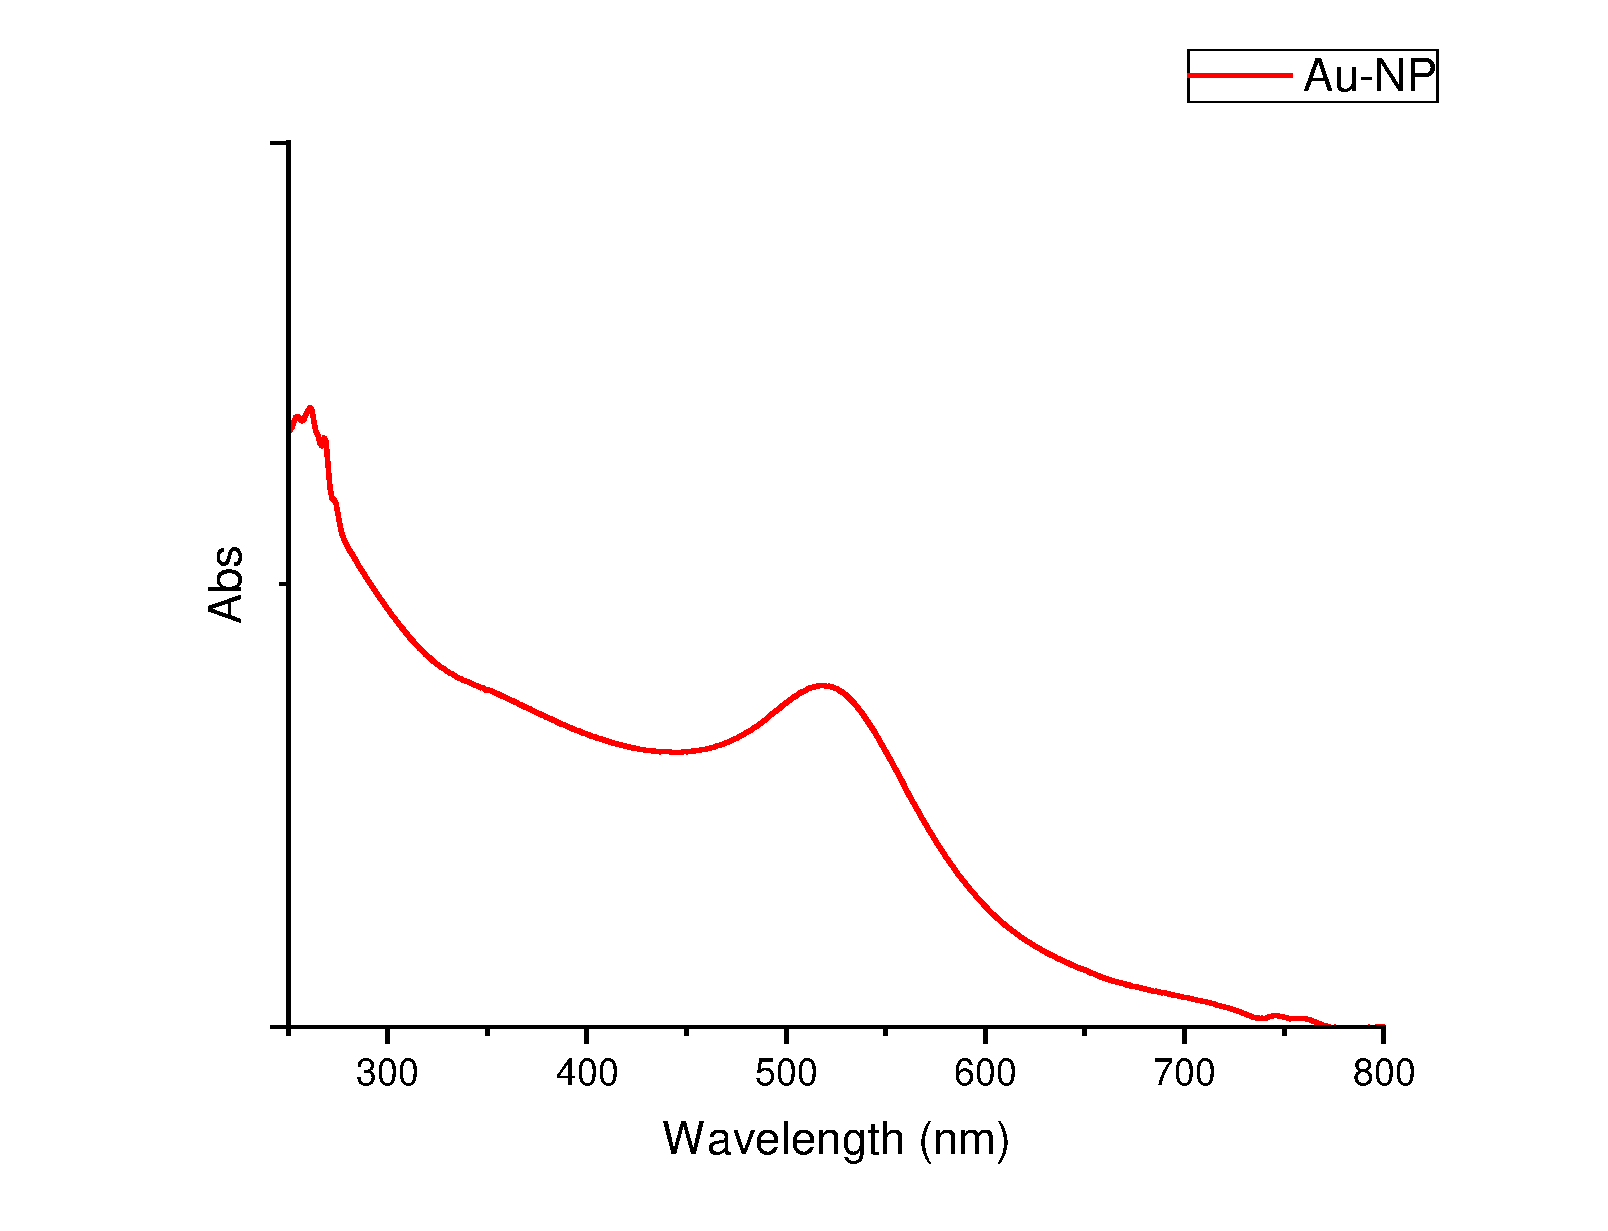
\includegraphics[width=0.6\textwidth]{Bilder/Gold-NP-Organisch} 	
		\caption{Absorptionsspektrum der Goldnanopartikel in Hexan gemessen.}
		\label{fig:UV-AuNP}
	\end{figure}
	
	\begin{figure}[htbp]
		\centering
		\subfloat[\label{fig:TEM-Au-Hex}]{%
			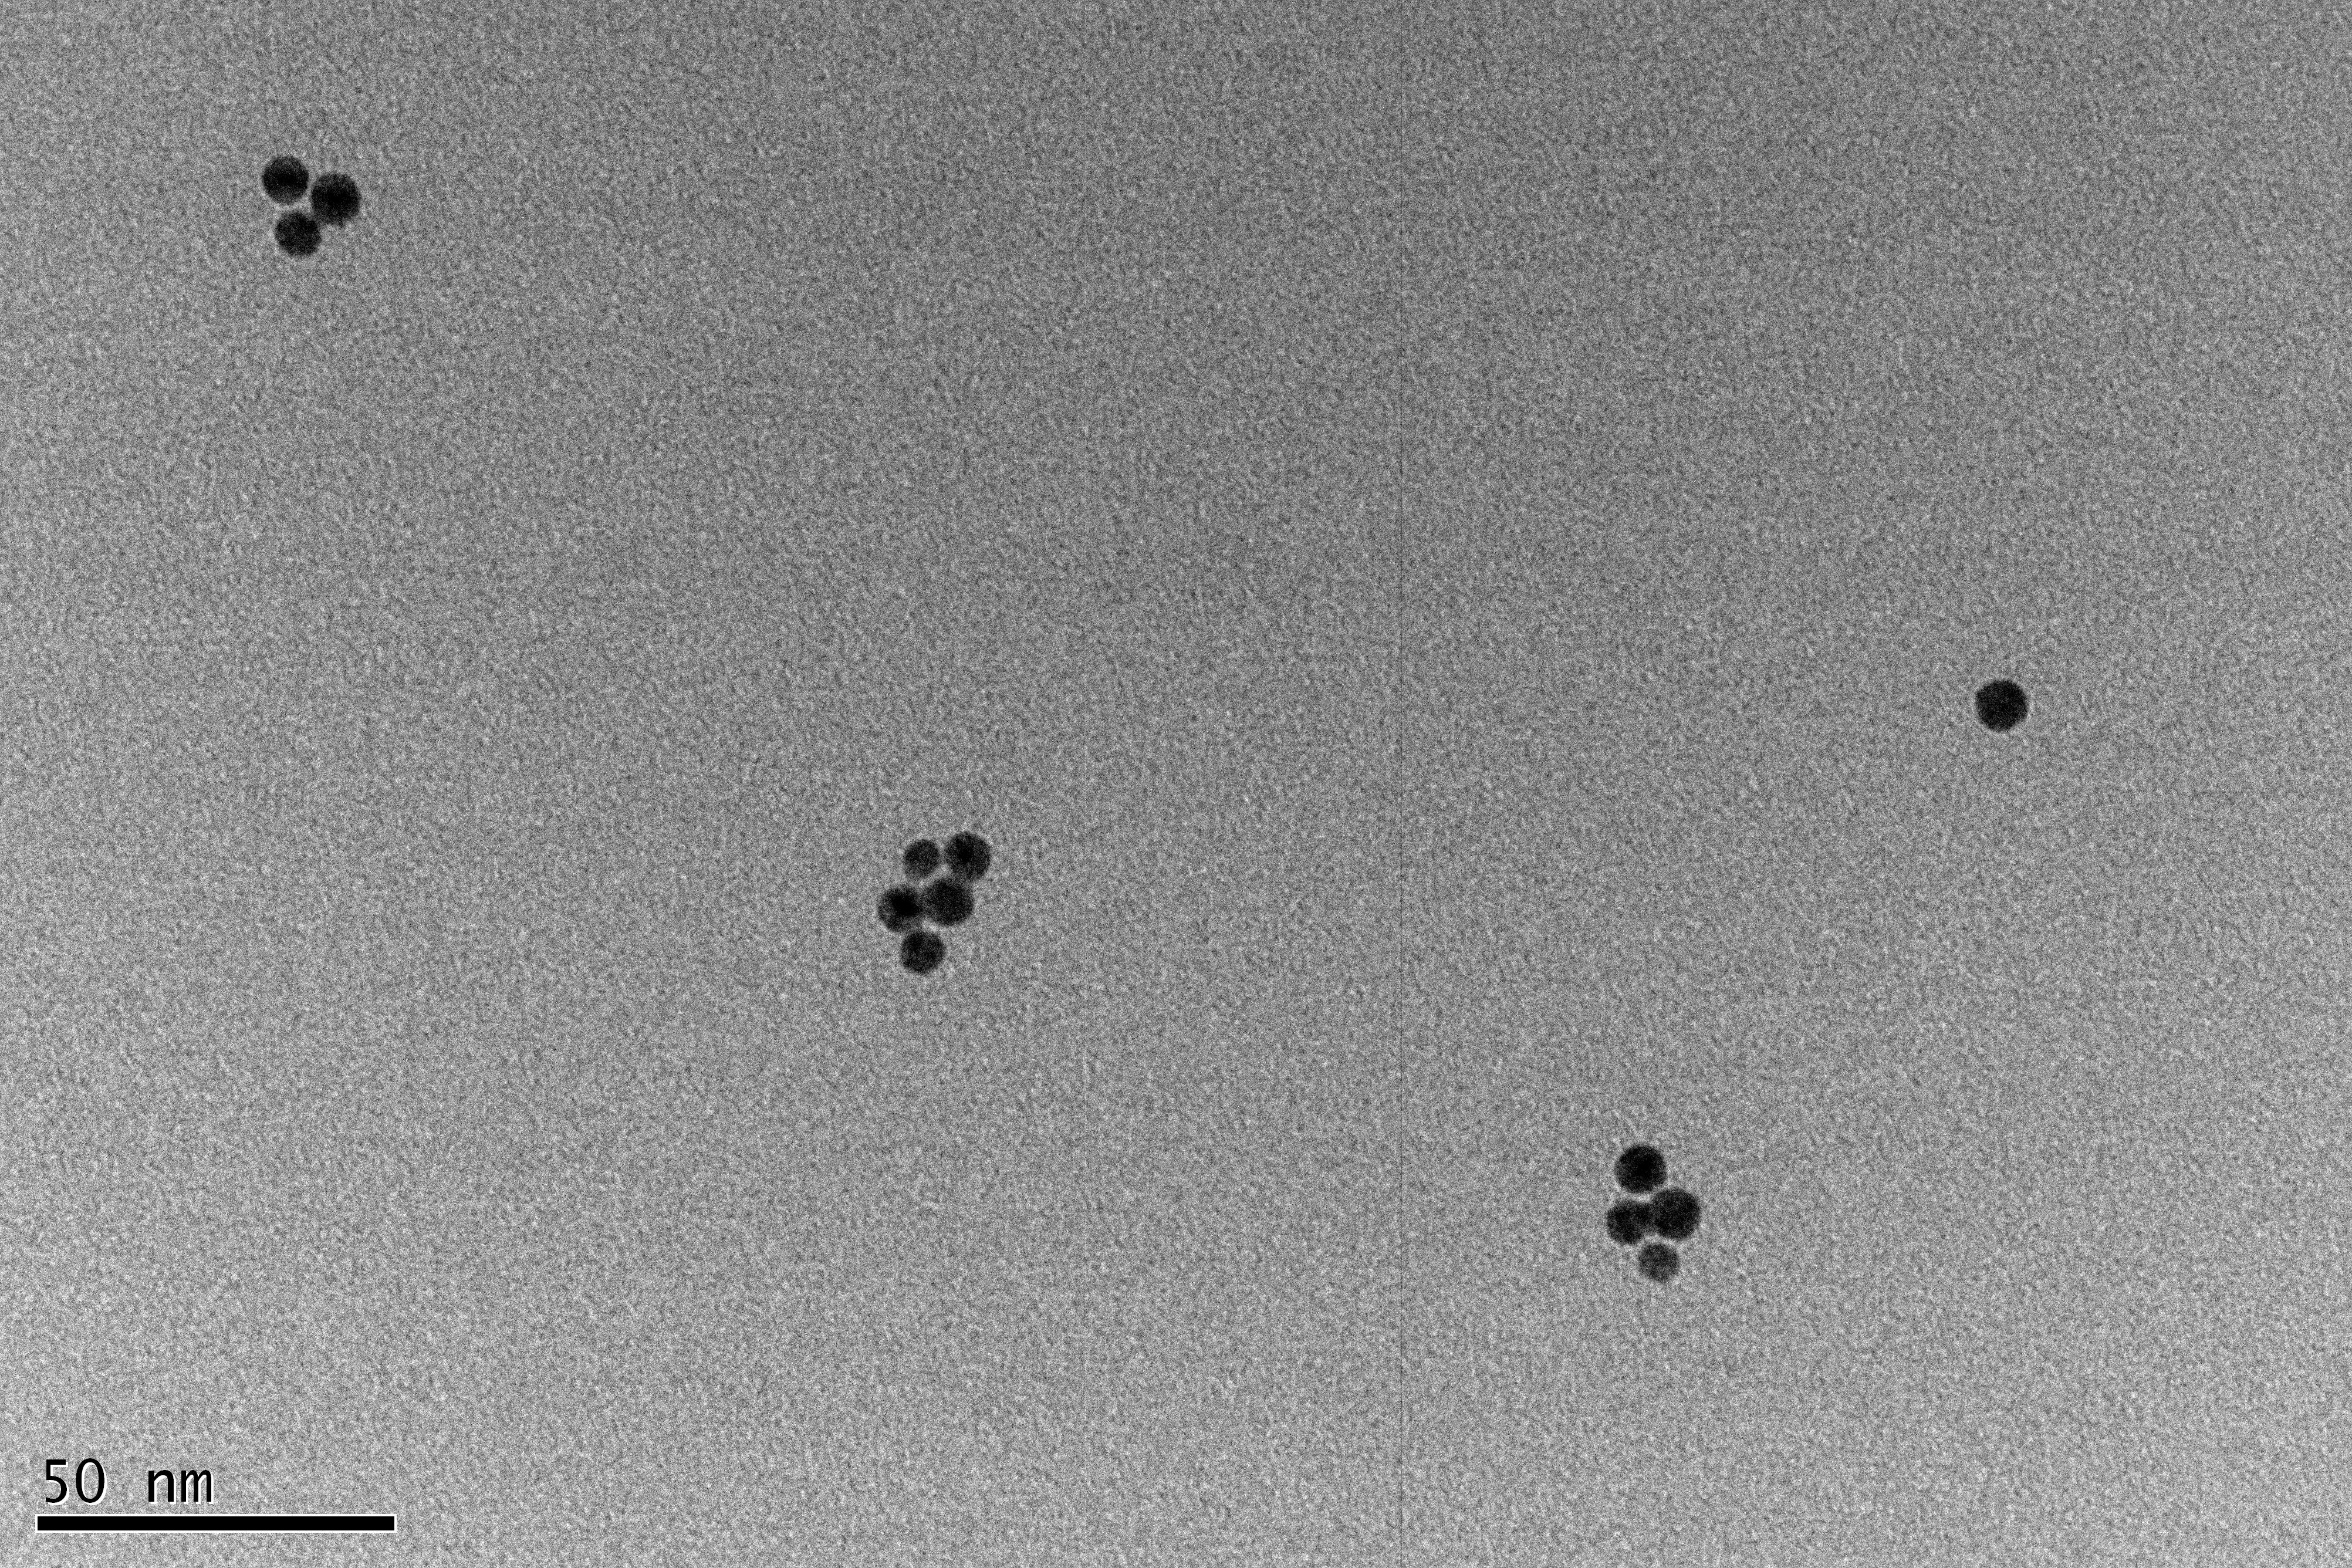
\includegraphics[width=0.45\linewidth]{Bilder/TEM-Au-Hex}}
		\subfloat[\label{fig:Size-Gold-NP}]{%
			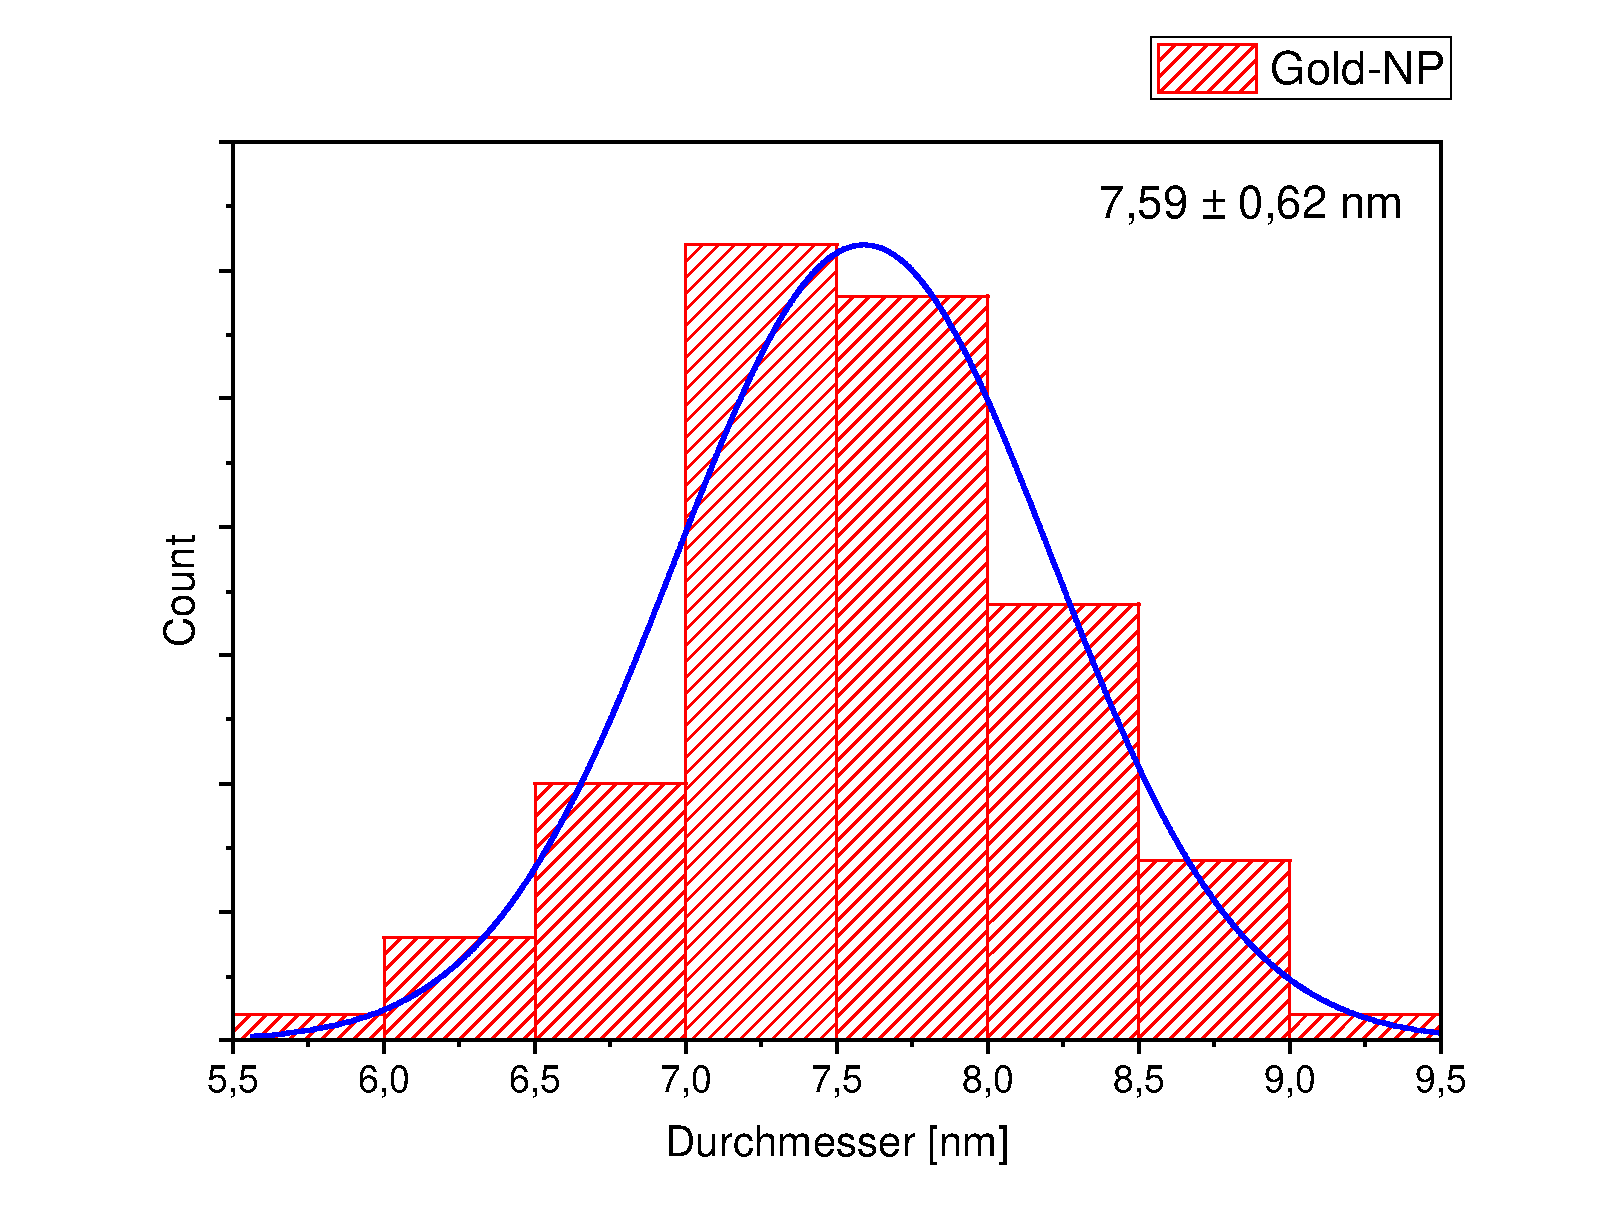
\includegraphics[width=0.45\linewidth]{Bilder/Size-Gold-NP-Organisch}}
		\caption{\emph{(a)}: TEM-Aufnahme der Gold-NP und \emph{(b)}: Größenverteilung}
		\label{fig:TEM-Au-Hex-2}
	\end{figure}

	

	
	
\subsection{Synthese von CuS mit \ch{Cu[DDTC]2} und \ch{CuCl2}}

	Bei der Synthese von \ch{Cu[DDTC]2} und \ch{CuCl2} zeigt sich deutlich der Einfluss des \ch{CuCl2}. 
	Während bei reinem \ch{Cu[DDTC]2} die Partikel auf eine Größe von über \SI{300}{\nano\meter} wachsen und es dementsprechend wenig Partikel gibt, zeigen die TEM-Aufnahmen, die in \cref{fig:TEM-CuCl} gezeigt sind, hier dass es zu vielen kleinen Partikeln in der Größe von Quantenpunkten kommt.
	
	\begin{figure}[H]
		\centering
		\subfloat[\label{fig:CuCl-1}]{%
		\includegraphics[width=0.45\linewidth]{Bilder/CuCl-1}}
		\subfloat[\label{fig:CuCl-2}]{%
		\includegraphics[width=0.45\linewidth]{Bilder/CuCl-2}}	
		\caption{TEM-Bilder von CuS-Nanopartikel, aus einem Gemisch von 80\% \ch{Cu[DDTC]2} und 20\% \ch{CuCl2}.}
		\label{fig:TEM-CuCl}
	\end{figure}
	
\subsection{Synthese von Kupfersulfid in Anwesenheit von Goldnanopartikeln}

	Um das Nukleationsverhalten bei der CuS-Synthese zu Untersuchen, wurde diese Reaktion in Anwesenheit von Goldnanopartikeln in verschiedenen Verhältnissen untersucht.
	Es wurden von diesen Mischungen jeweils UV-vis-NIR-Absorptionsmessungen vorgenommen und von ausgewählten Proben TEM-Aufnahmen und XRD-Messungen vorgenommen.
	
	\begin{figure}[htbp]
		\centering
		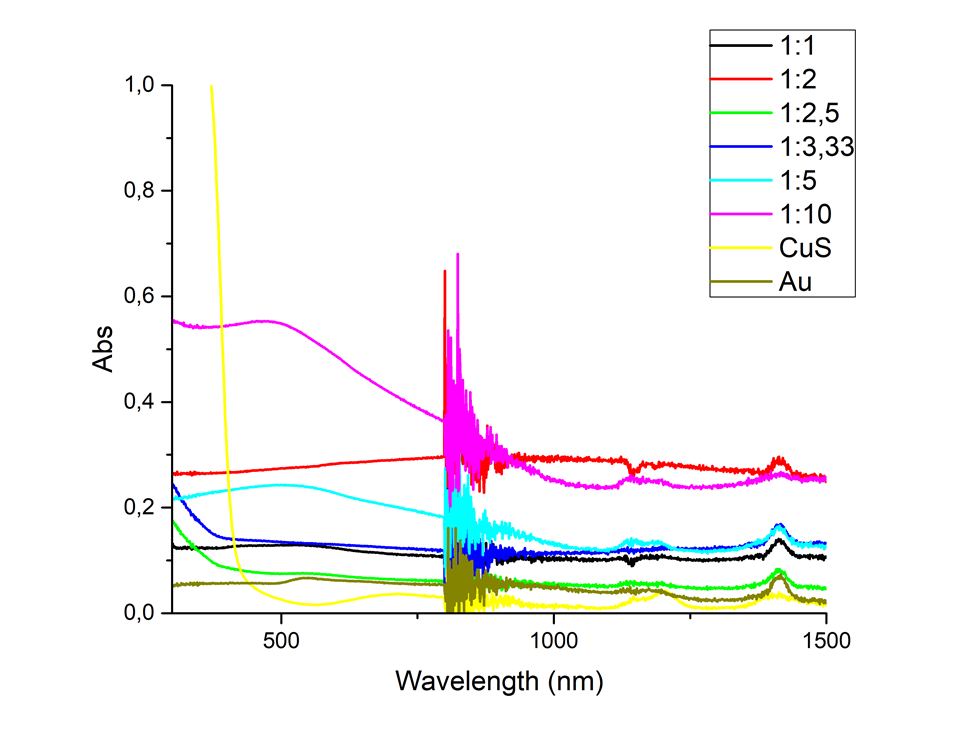
\includegraphics[width=0.6\textwidth]{Bilder/UV-AuCu-Konz} 	
		\caption{UV-vis-NIR-Messungen der Proben mit verschieden Mischungsverhältnissen von Au:\ch{Cu[DDTC]2} in Toluol (gemessen in Ulbrichtkugel).}
		\label{fig:UV-AuCu}
	\end{figure}
	
	Die Absorptionsmessungen in \cref{fig:UV-AuCu} zeigen, dass bei den Mischungen mit geringem Goldanteil ein Maximum bei etwa \SI{500}{\nano\meter} entsteht, dass mit steigendem Goldanteil abnimmt.
	Dies könnte das Plasmon der Goldpartikel sein.
	Interessanterweise ist das Maximum bei diesen Mischungen leicht blauverschoben und teilweise ausgeprägter als bei einer Vergleichsprobe, bei der die gleiche Reaktion ohne \ch{Cu[DDTC]2} und nur mit der Gold-NP-Lösung durchgeführt wurde.
	
	Die TEM-Aufnahmen zeigen, dass bei den Proben sowohl mit einem hohen als auch bei einem niedrigen Au:\ch{Cu[DDTC]2}-Verhältnis es zu einzelnen kleinen Gruppen von Gold-NPs kommt, an denen sich nicht gebildet hat (\cref{fig:CuAu-10-10_2} bzw. \cref{fig:CuAu-10-1_2}).
	Bei geringem Goldanteil scheint ein Teil des \ch{Cu[DDTC]2} wie bei der Probe ohne Gold zu reinem hexagonalem CuS zu reagieren, wie \cref{fig:CuAu-10-1_3} zeigt.
	Insgesamt lässt sich hier aber erkennen, dass die CuS-Partikel in Anwesenheit von den Gold-NP sich deutlich anders ausbilden und es an einigen Stellen so aussieht, als währen dort Goldpartikel eingelagert, was besonders in \cref{fig:CuAu-10-1_1} zu erkennen ist.
	
	\begin{figure}[htbp]
		\centering
		\subfloat[\label{fig:CuAu-10-10_1}]{%
			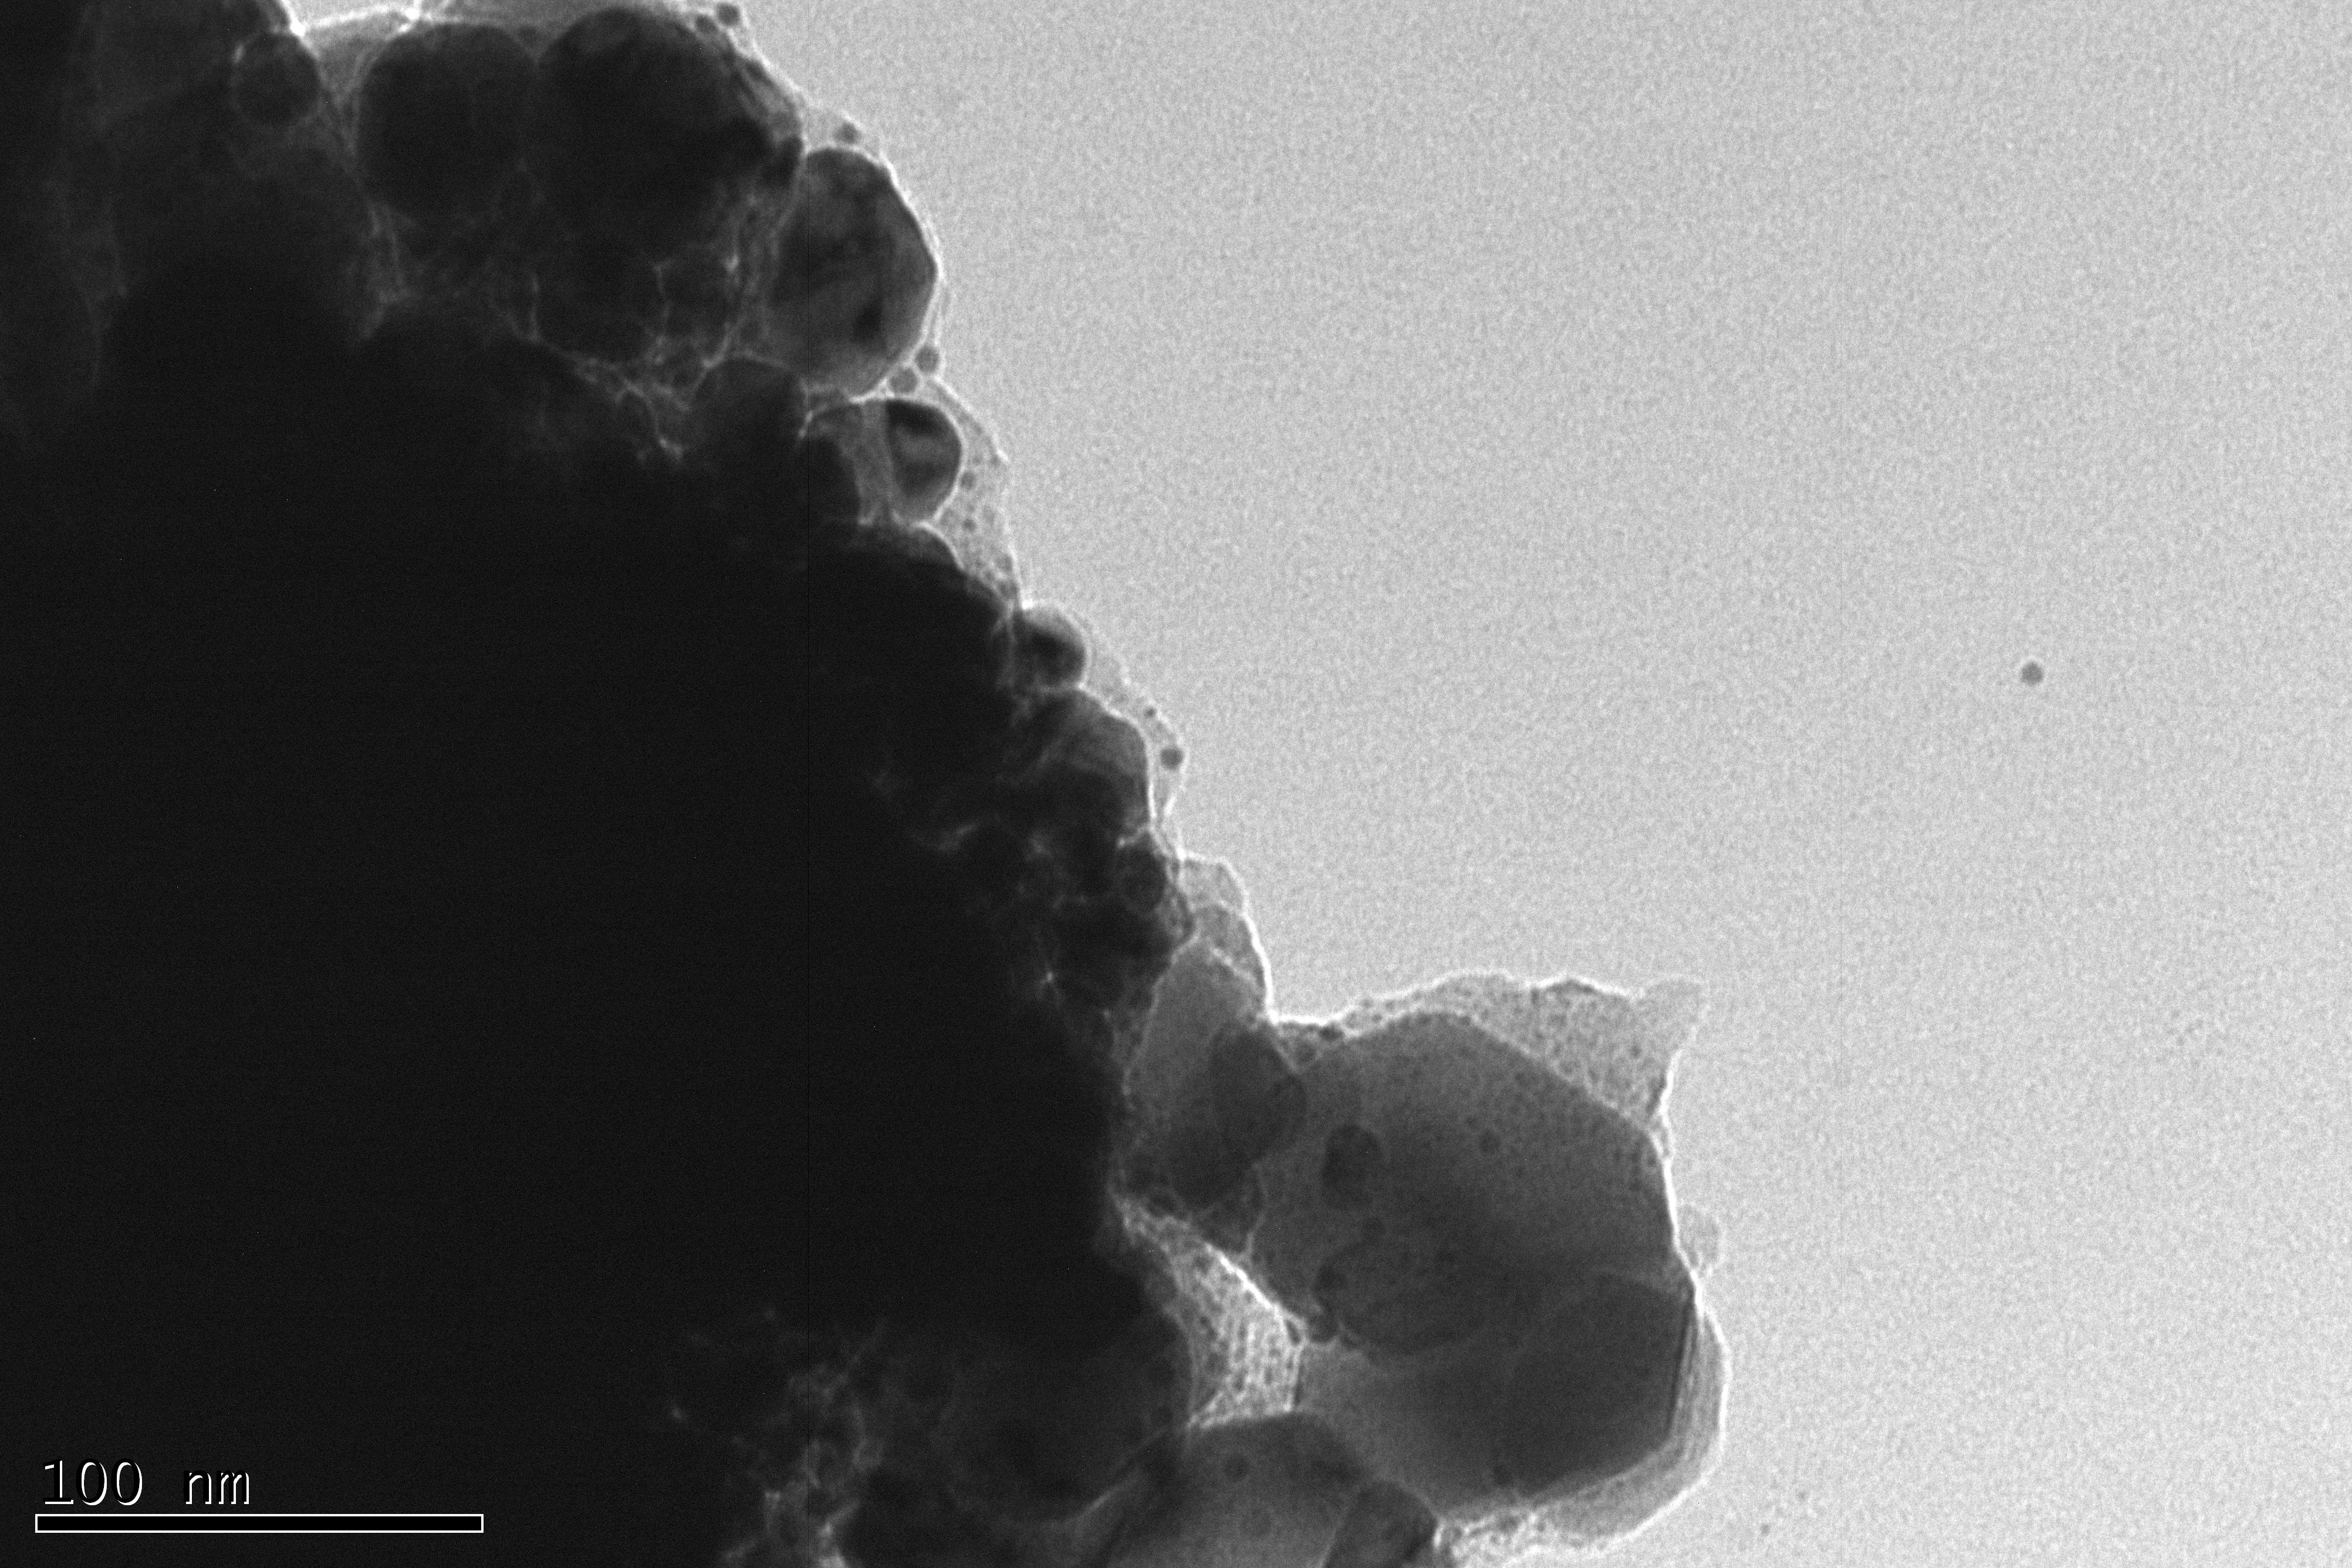
\includegraphics[width=0.33\linewidth]{Bilder/CuAu-10-10_1}}
		\subfloat[\label{fig:CuAu-10-10_2}]{%
			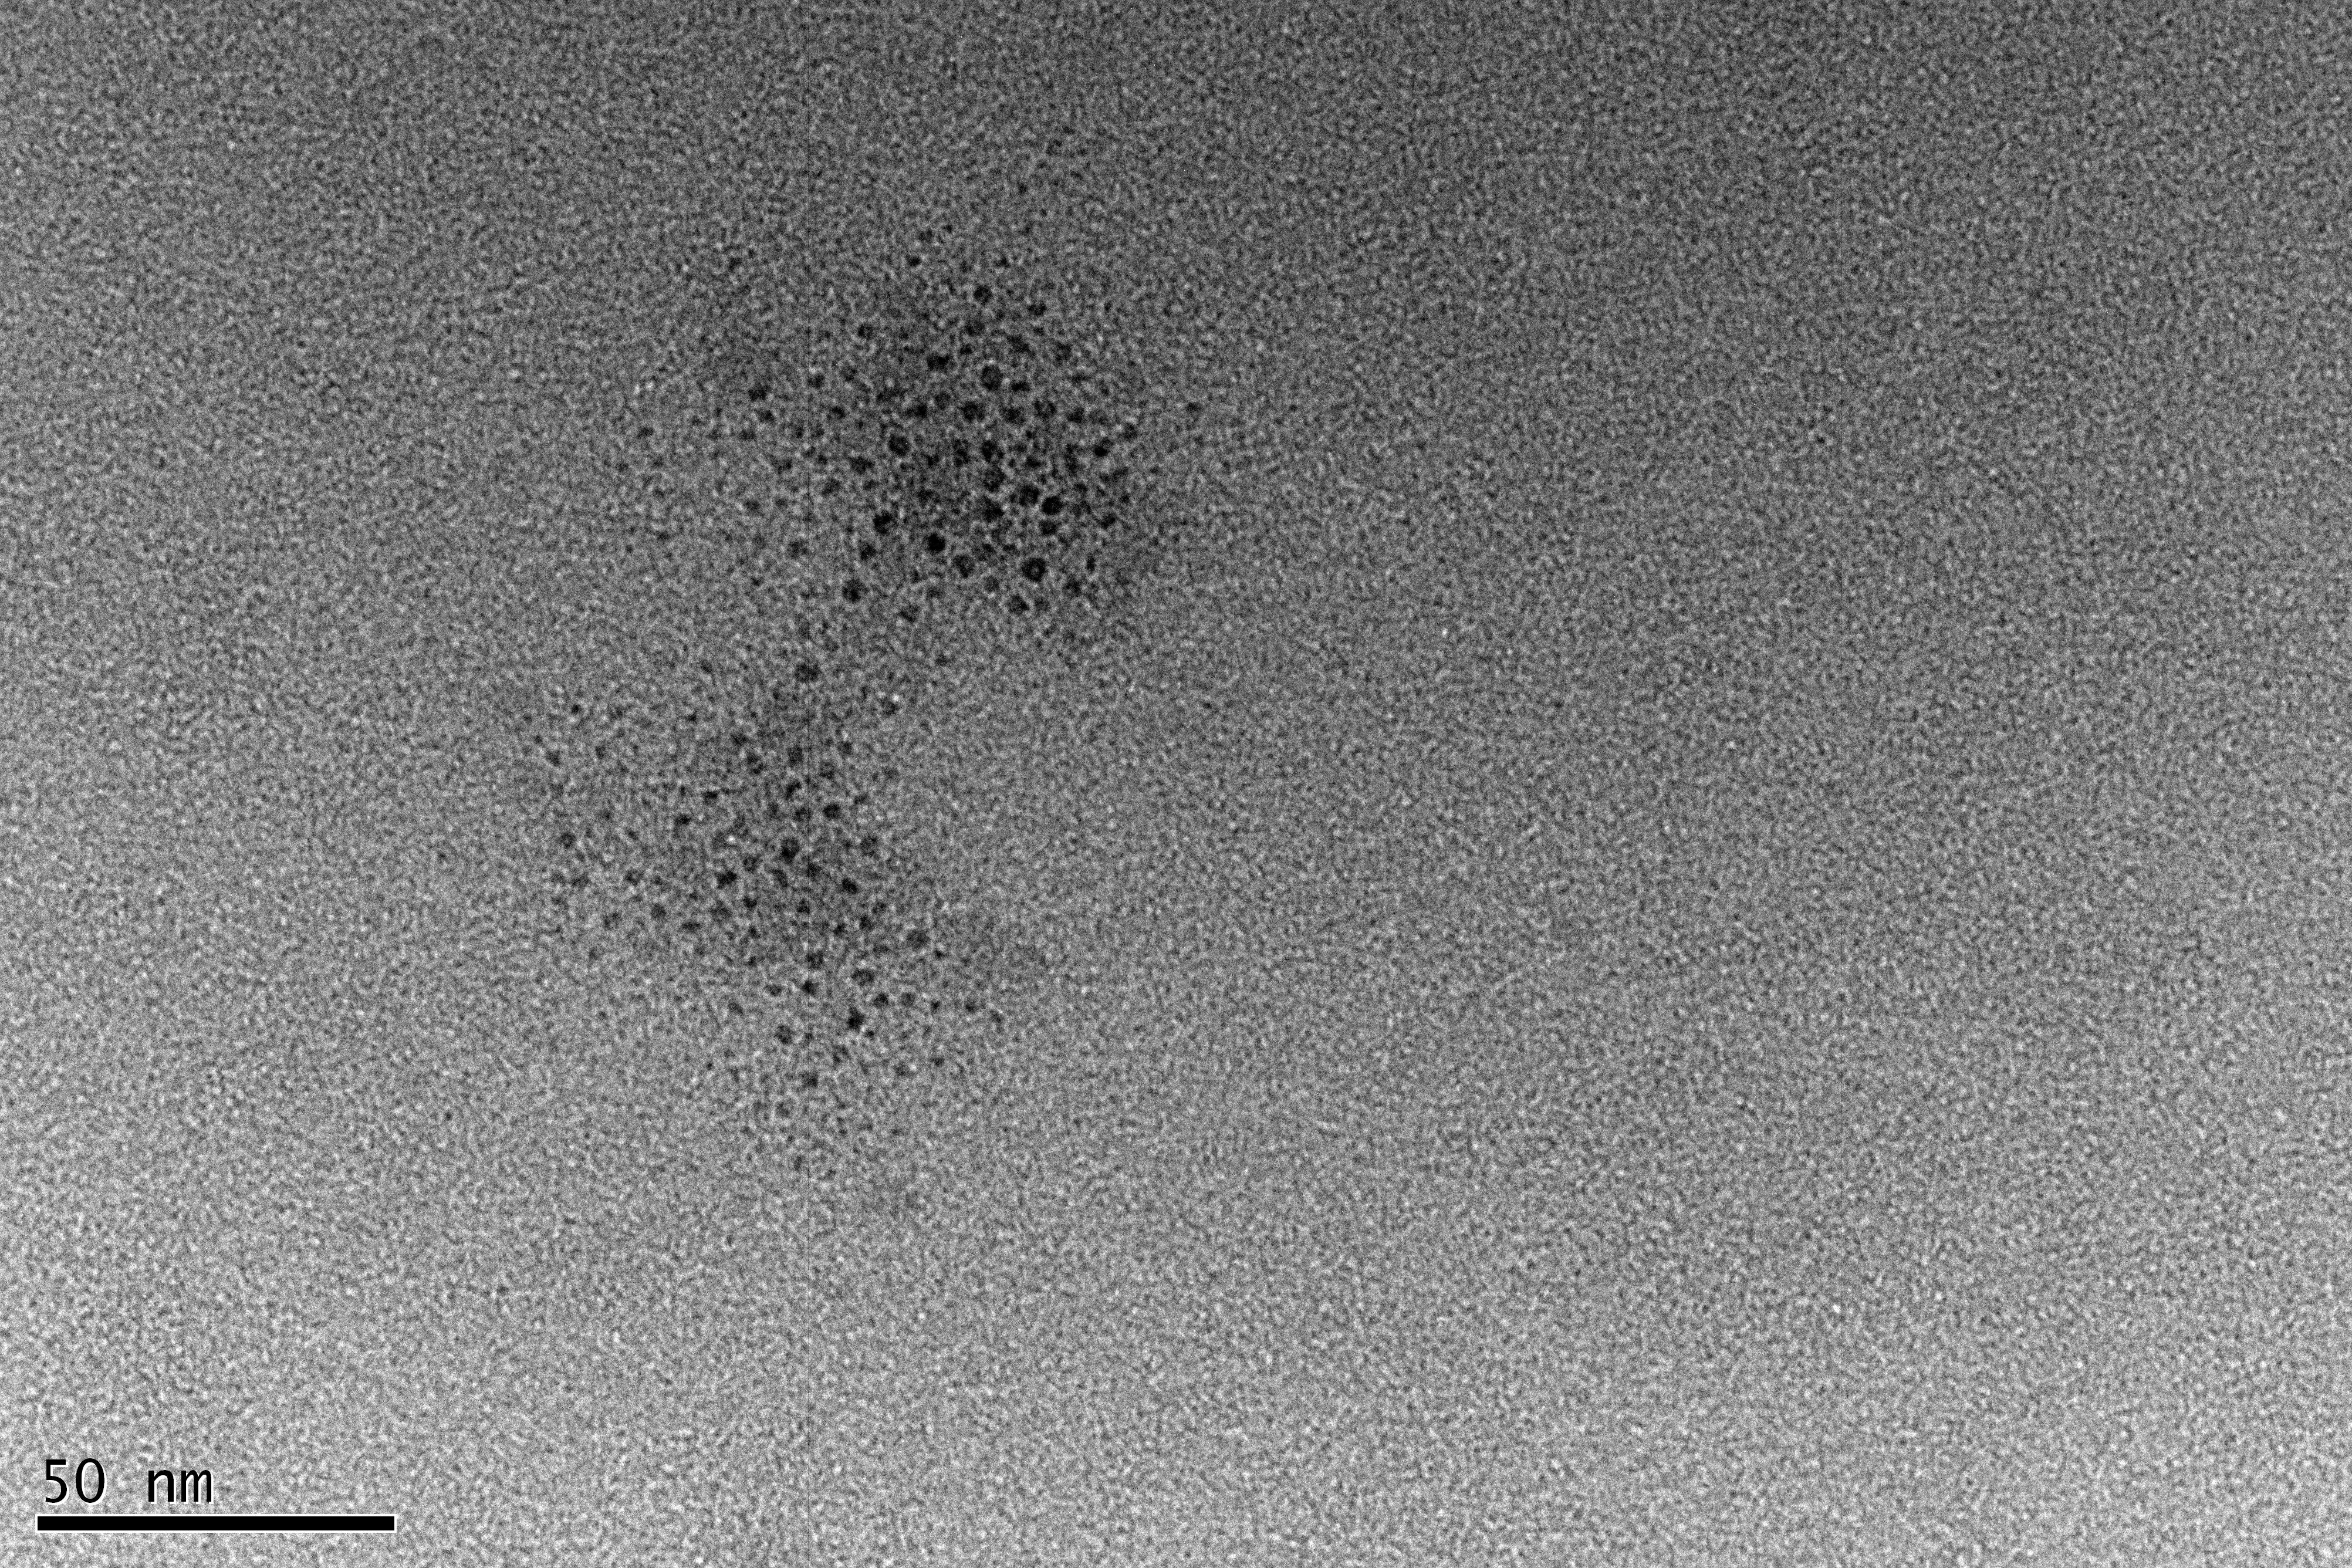
\includegraphics[width=0.33\linewidth]{Bilder/CuAu-10-10_2}}
		\subfloat[\label{fig:CuAu-10-10_3}]{%
			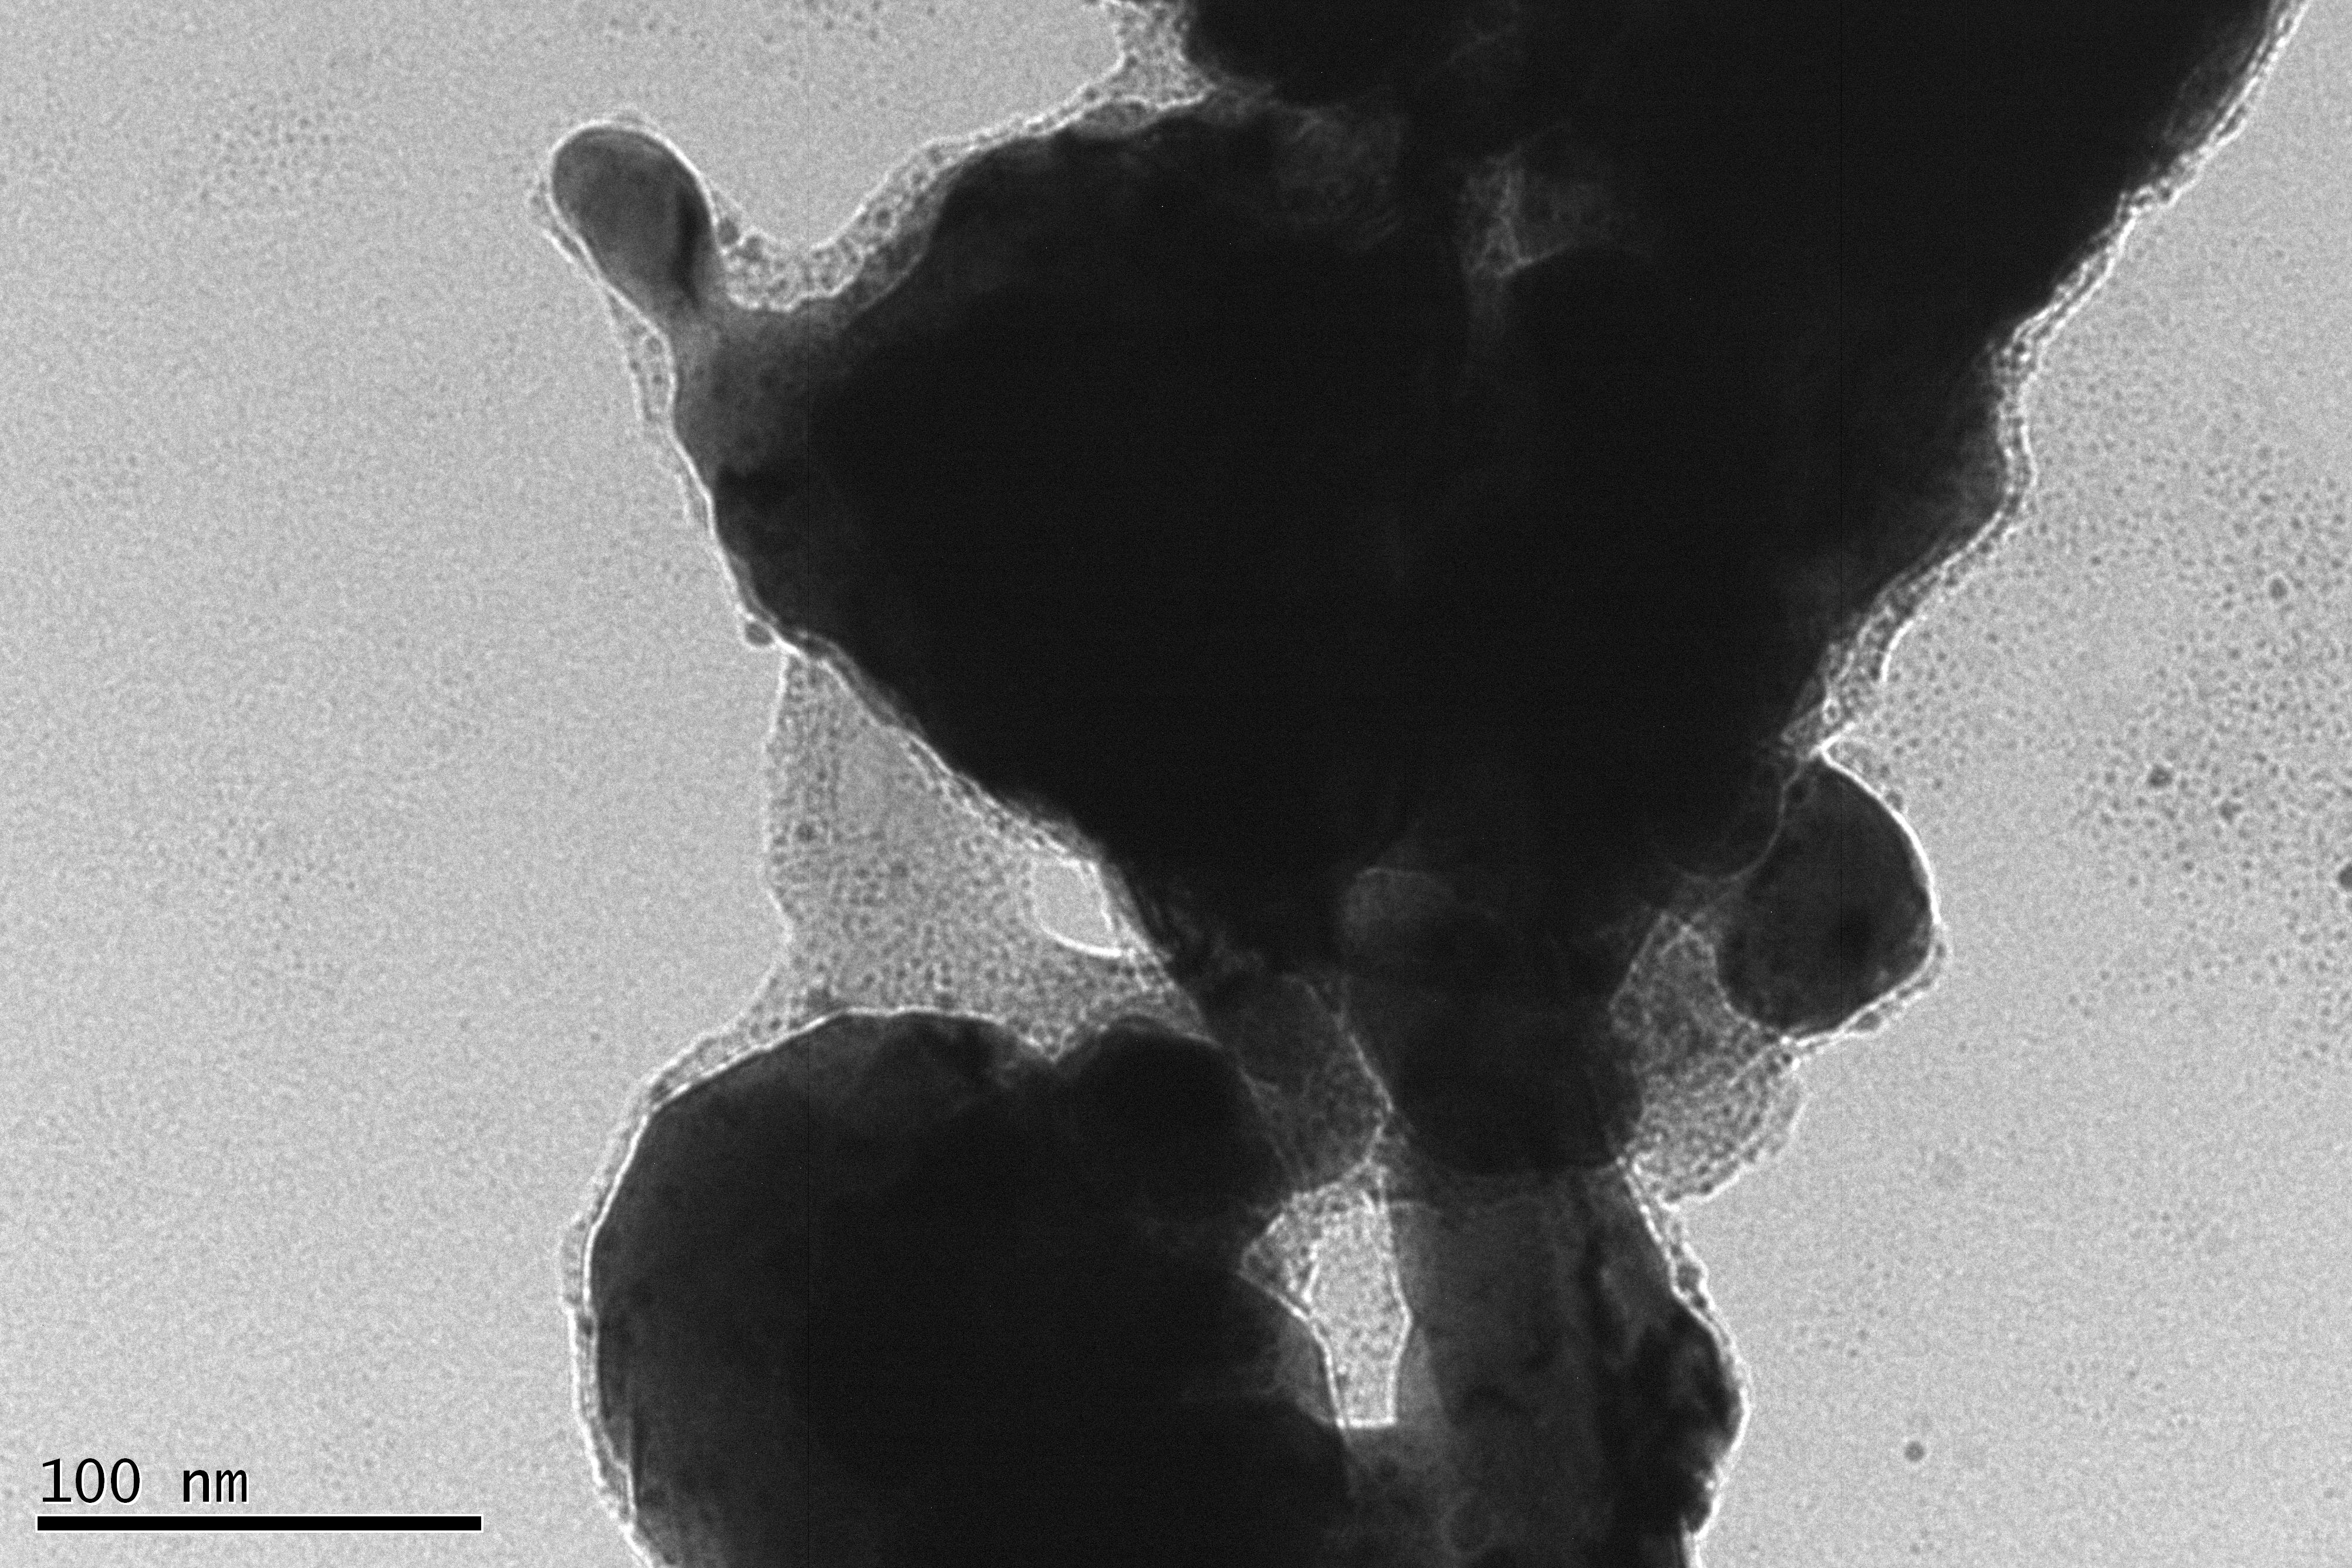
\includegraphics[width=0.33\linewidth]{Bilder/CuAu-10-10_3}}
		\caption{TEM-Aufnahmen der Probe mit einem Mengenverhältnis von 1:1 Au:\ch{Cu[DDTC]2}.}
		\label{fig:TEM-CuAu-10-10}
	\end{figure}
	
	\begin{figure}[htbp]
		\centering
		\subfloat[\label{fig:CuAu-10-1_1}]{%
			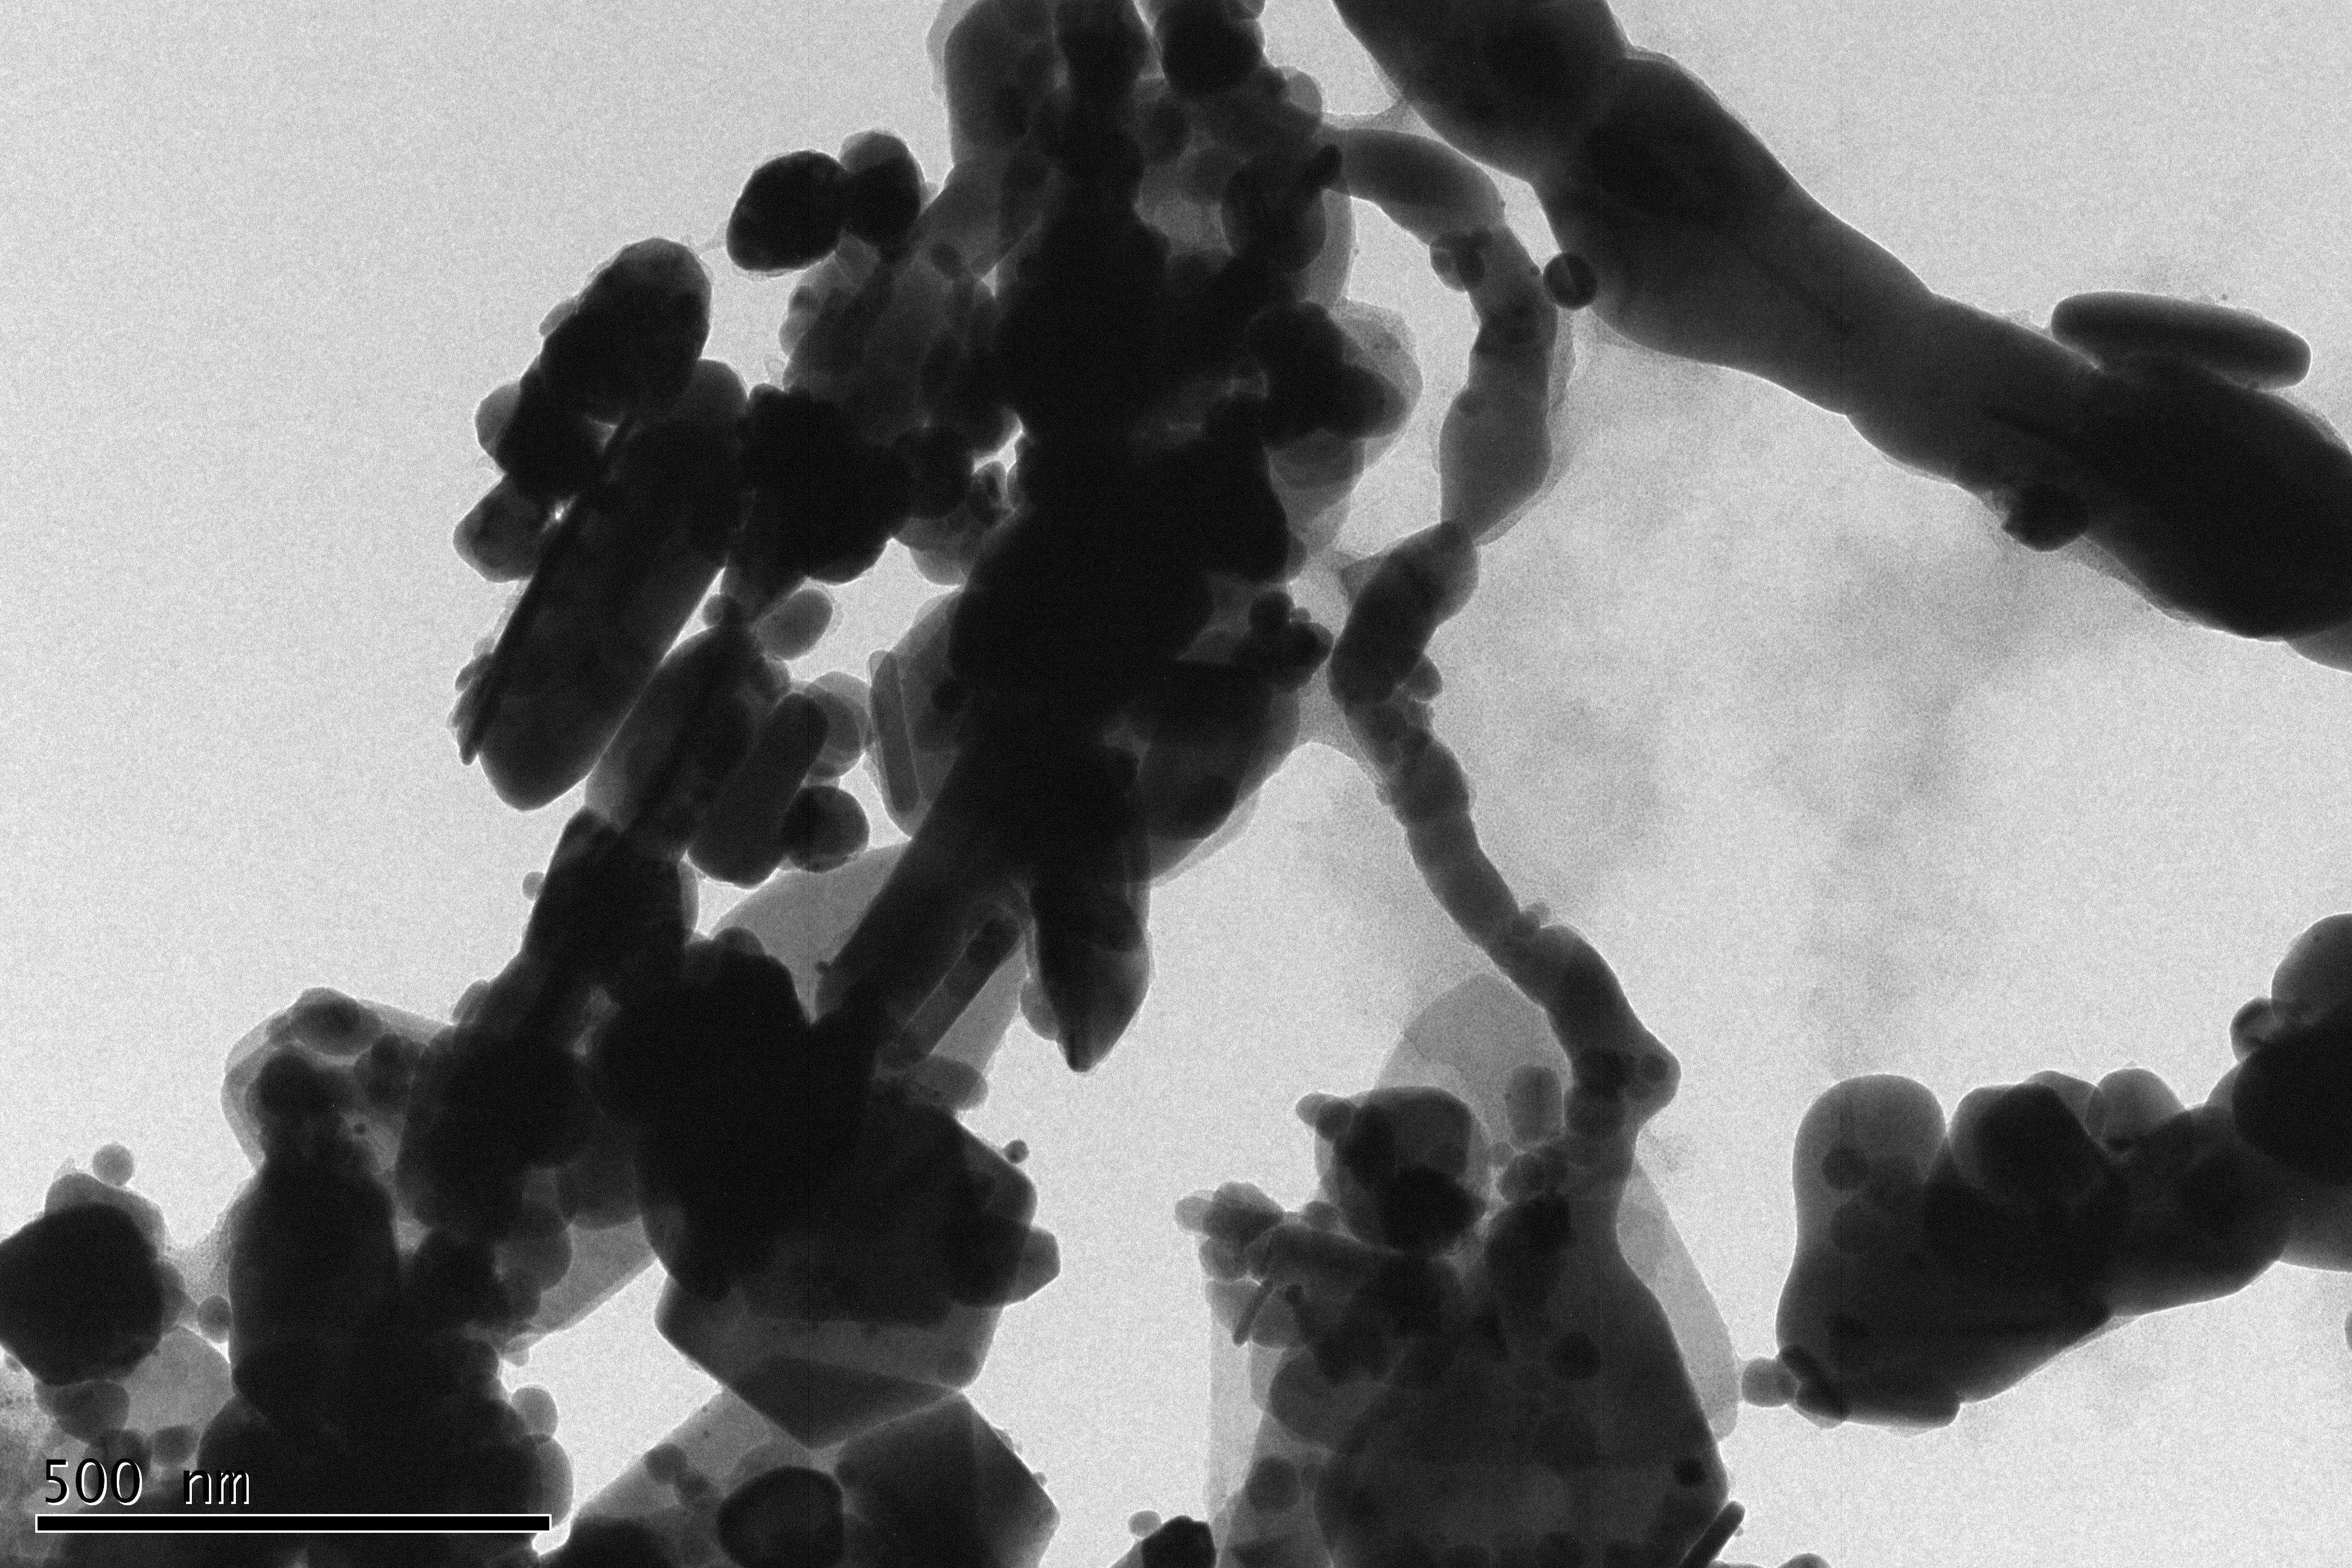
\includegraphics[width=0.33\linewidth]{Bilder/CuAu-10-1_1}}
		\subfloat[\label{fig:CuAu-10-1_2}]{%
			\includegraphics[width=0.33\linewidth]{Bilder/CuAu-10-1_2}}
		\subfloat[\label{fig:CuAu-10-1_3}]{%
			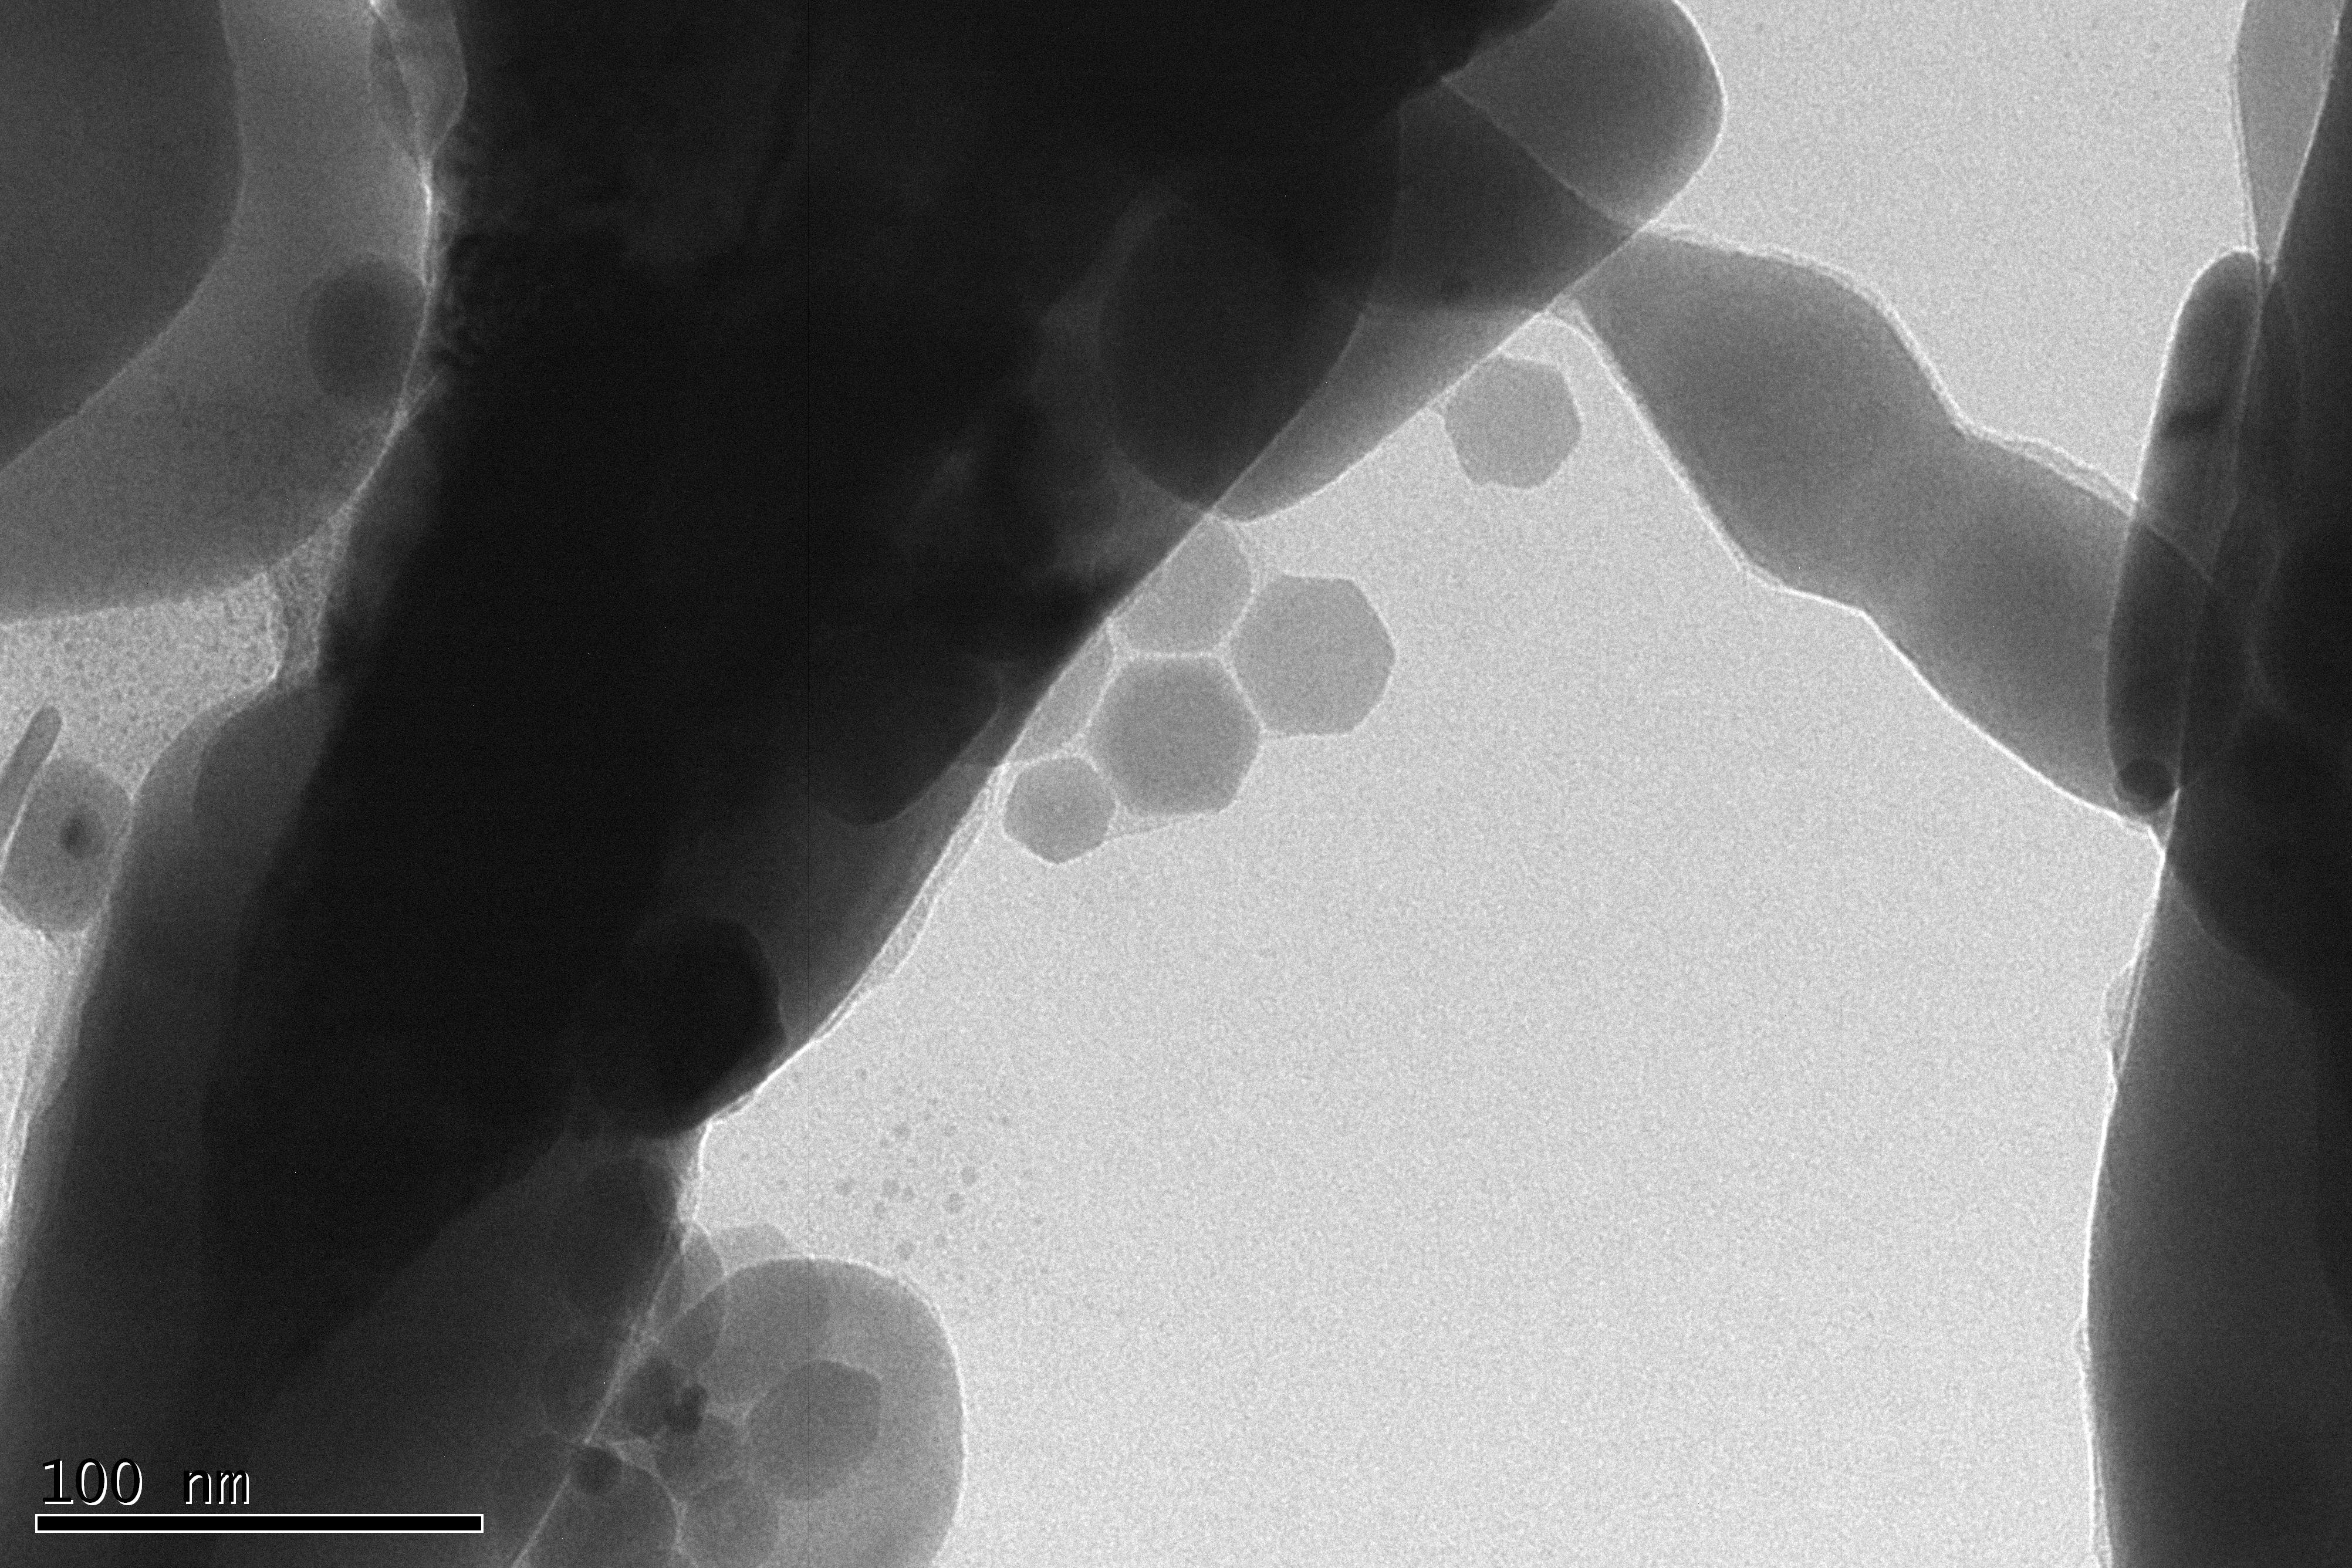
\includegraphics[width=0.33\linewidth]{Bilder/CuAu-10-1_3}}
		\caption{TEM-Aufnahmen der Probe mit einem Mengenverhältnis von 1:10 Au:\ch{Cu[DDTC]2}.}
		\label{fig:TEM-CuAu-10-1}
	\end{figure}
	
	Von den Mengenverhältnis 1:2 und 1:10 Au:\ch{Cu[DDTC]2} wurde zudem eine XRD-Messung vorgenommen, das in \cref{fig:XRD} gezeigt ist.
	Die 1:10-Probe ziegte einige scharfe Peaks zwischen 10° und 25°, die allerdings weder dem CuS, noch den Edukten zugeordnet werden können.
	Es konnte auch sonst keine Struktur gefunden werden, die hierfür in Frage kommt, die aus Kupfer und Schwefel besteht.
	Das XRD beim  Mengenverhältnis von 1:2 Au:\ch{Cu[DDTC]2} zeigt ein deutlich anderes Diffraktogramm, mit einem breiten Peak bei etwa 41° und zwei kleinen bei 46° und 48°. Auch diese passen zu keinem der Produkte oder Edukte.
	\todo{vielleicht Verschiebung des Gold-Peaks?}
	Es liegt der Verdacht nah, dass die Proben nicht kristallin genug waren um Signale im XRD zu erzeugen.
	
	\begin{figure}[H]
		\centering
		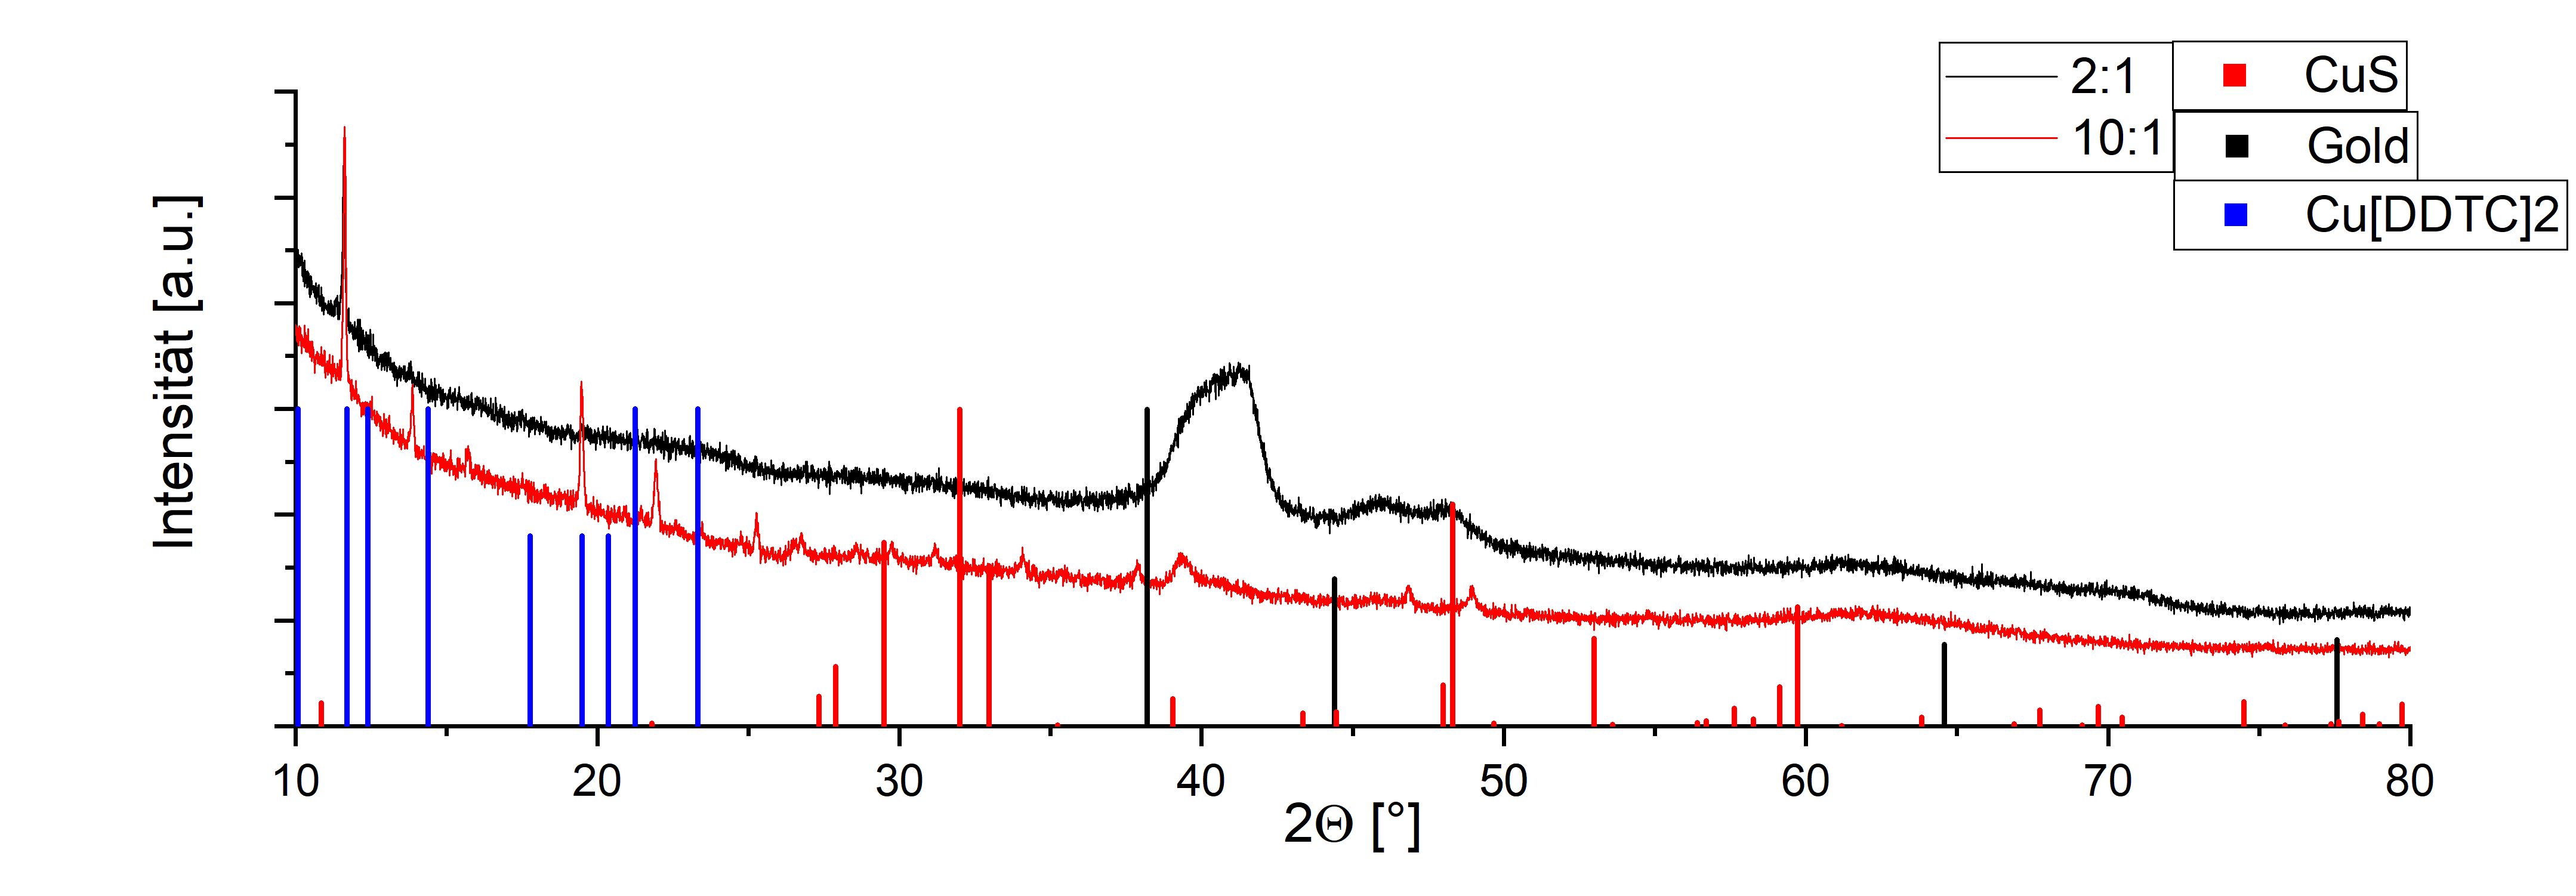
\includegraphics[width=\textwidth]{Bilder/XRD-CuS} 	
		\caption{XRD-Messung von Proben mit Mengenverhältnissen 1:2 und 1:10 Au:\ch{Cu[DDTC]2}.}
		\label{fig:XRD}
	\end{figure}
	
	
	
	

\subsection{Synthese der Gele}
	
	\subsubsection{Untersuchung von Hydrogelen durch Yttrium und Ytterbium}
	
		Bei fast allen Versuchen konnte nach einiger Zeit ein dunkler Niederschlag erkannt werden und die Lösung entfärbte sich bei fast allen Proben.
		Wie in \cref{fig:0625Au-Gele} zu erkennen ist, sind bei niedrigen Gold-NP-Konzentrationen von \SI{0,625}{\gram\per\liter} sowohl Yttrium als auch Ytterbium in allen verwendeten Konzentrationen in der Lage die in kolloidaler Lösung vorhandenen Goldnanopartikel auszufällen.
		Bei höheren Goldkonzentrationen konnte ein deutlicher Unterschied zwischen Ytterbium und Yttrium festgestellt werden. 
		Währenddessen die Yttriumlösungen auch die höheren Gold-NP-Konzentrationen von \num{1,25} und \SI{2,5}{\gram\per\liter} komplett ausfällen konnte, war dies mit Ytterbium in gleicher Konzentration nicht möglich, wie in \cref{fig:1Y-Yb-Gele} durch die immer noch vorhandene Rotfärbung zu erkennen ist.
		
		\begin{figure}[htbp]
			\centering
			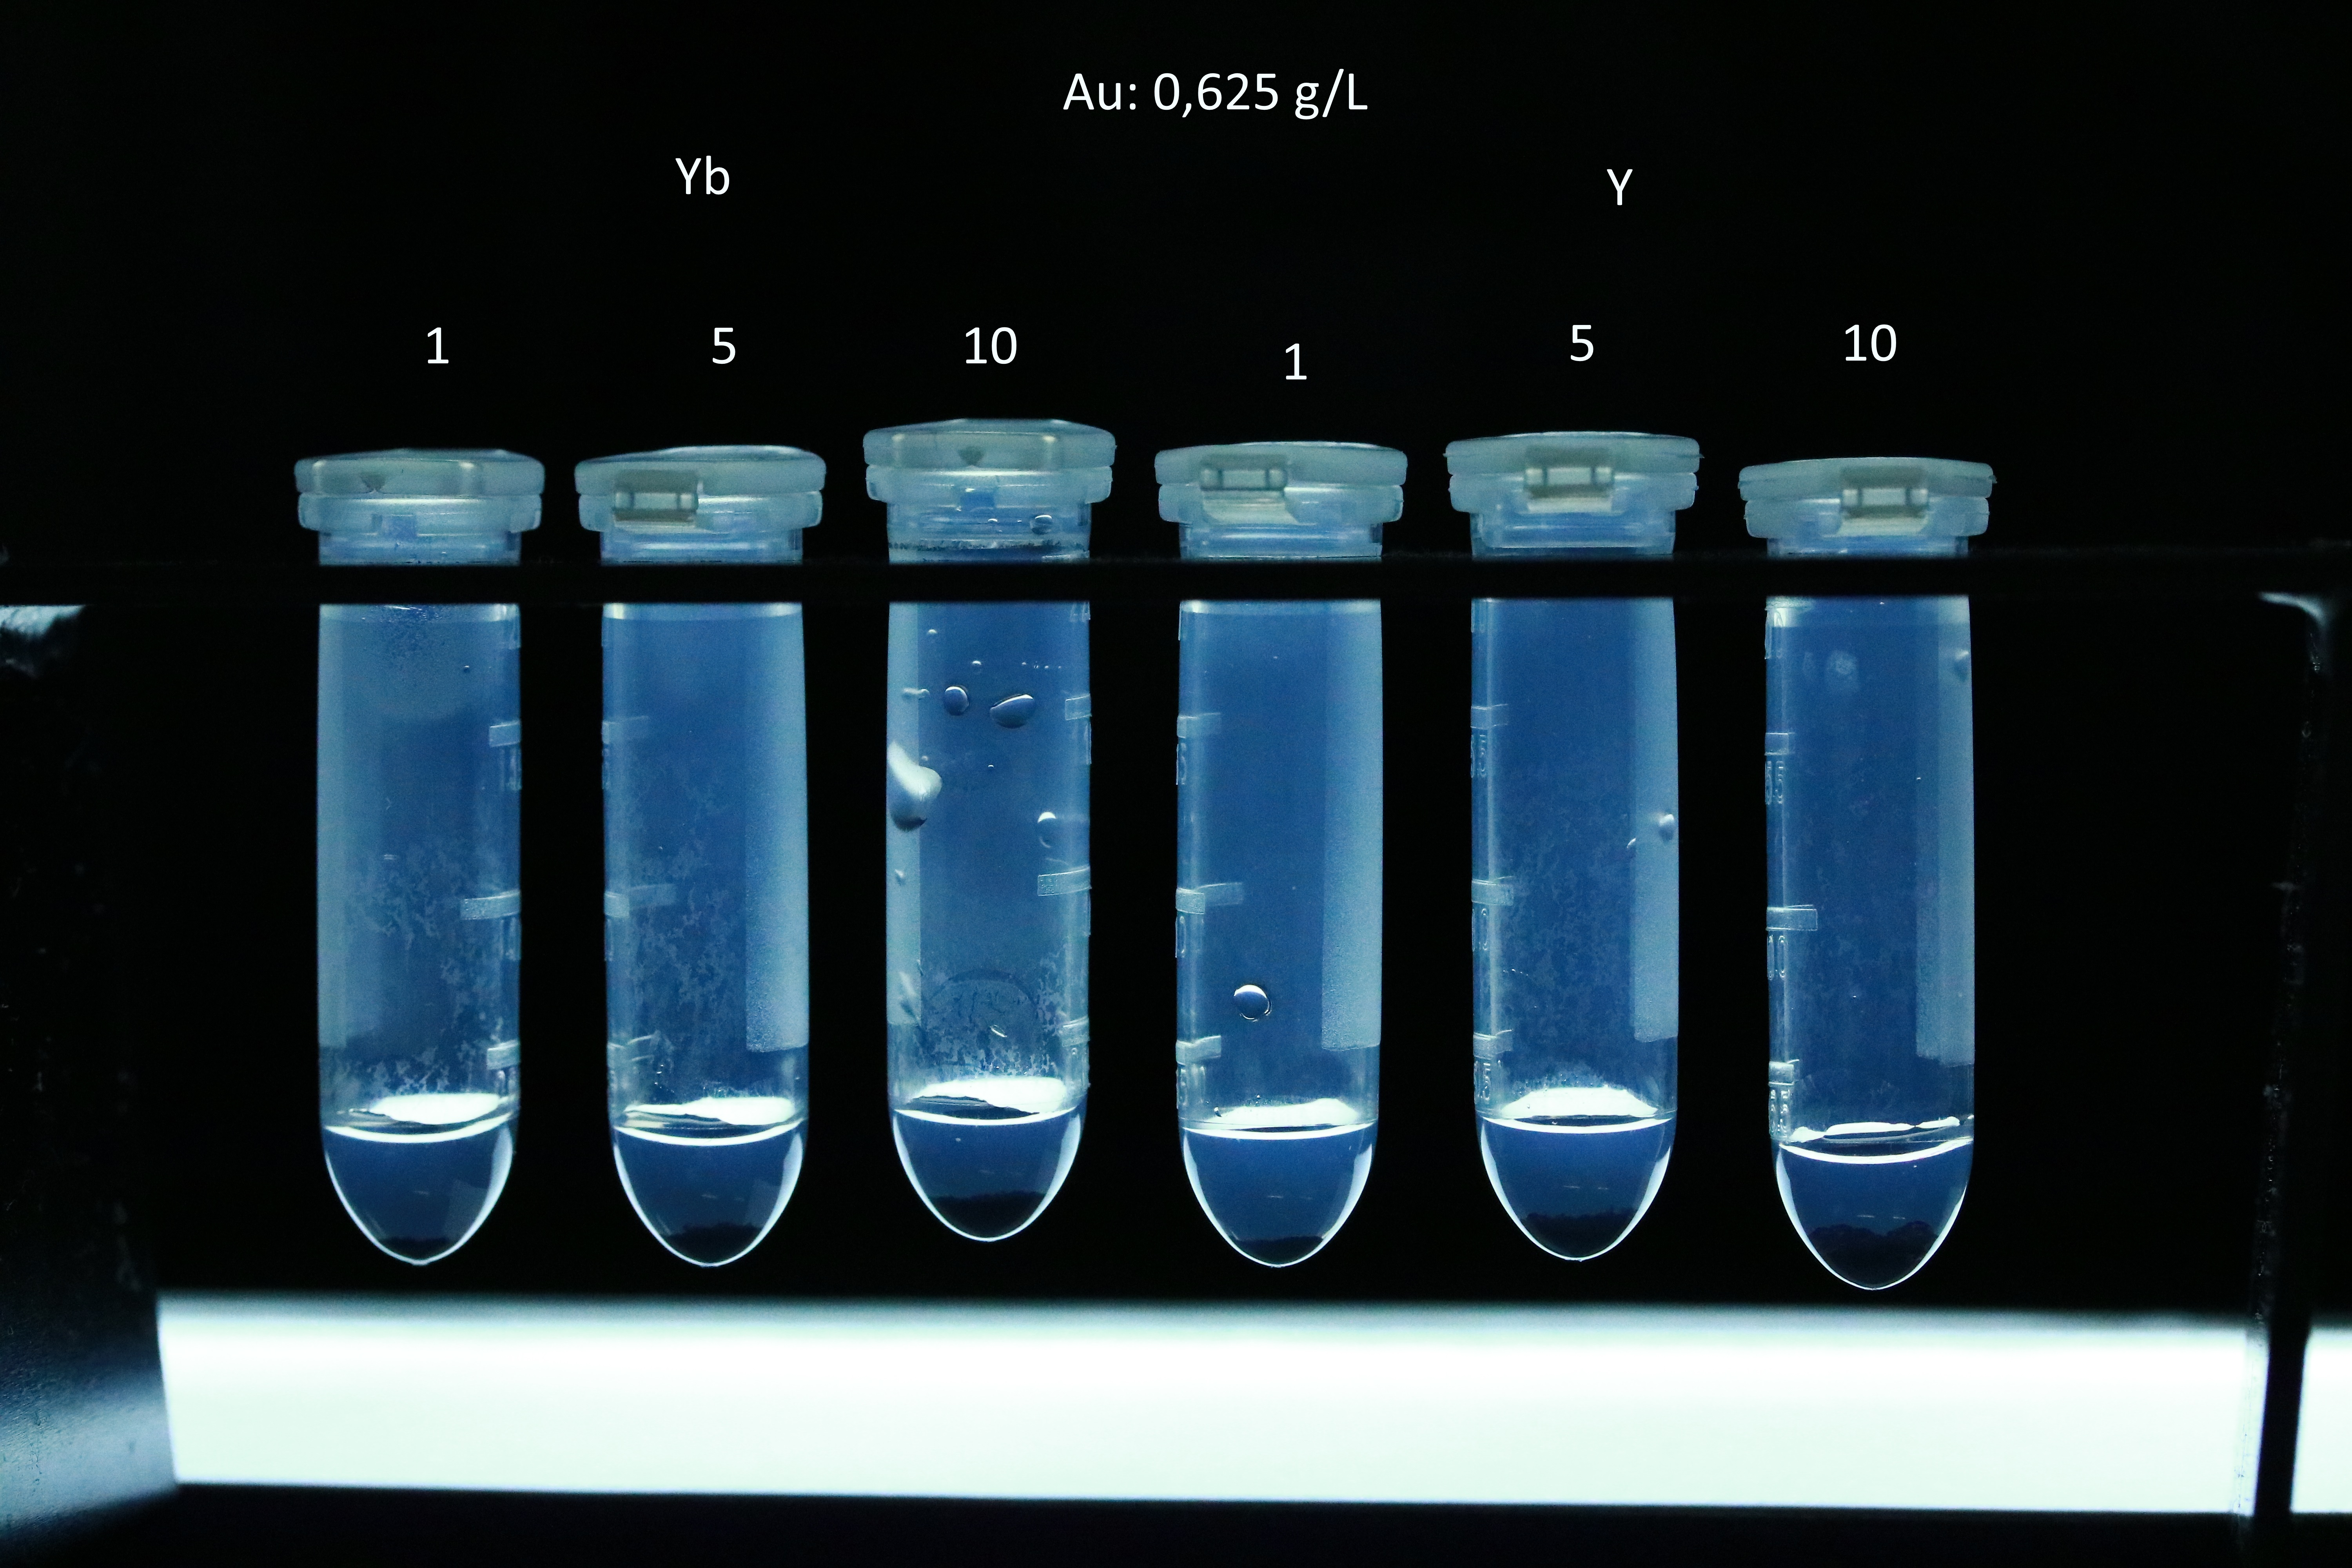
\includegraphics[width=0.6\textwidth]{Bilder/0625Au-Gele} 	
			\caption{Übersicht der Gele mit 0,625 g/L Goldlösung und Salzlösungen mit 1;5;10 mM Yb$^{3+}$ und Y$^{3+}$.}
			\label{fig:0625Au-Gele}
		\end{figure}
	
		\begin{figure}[htbp]
			\centering
			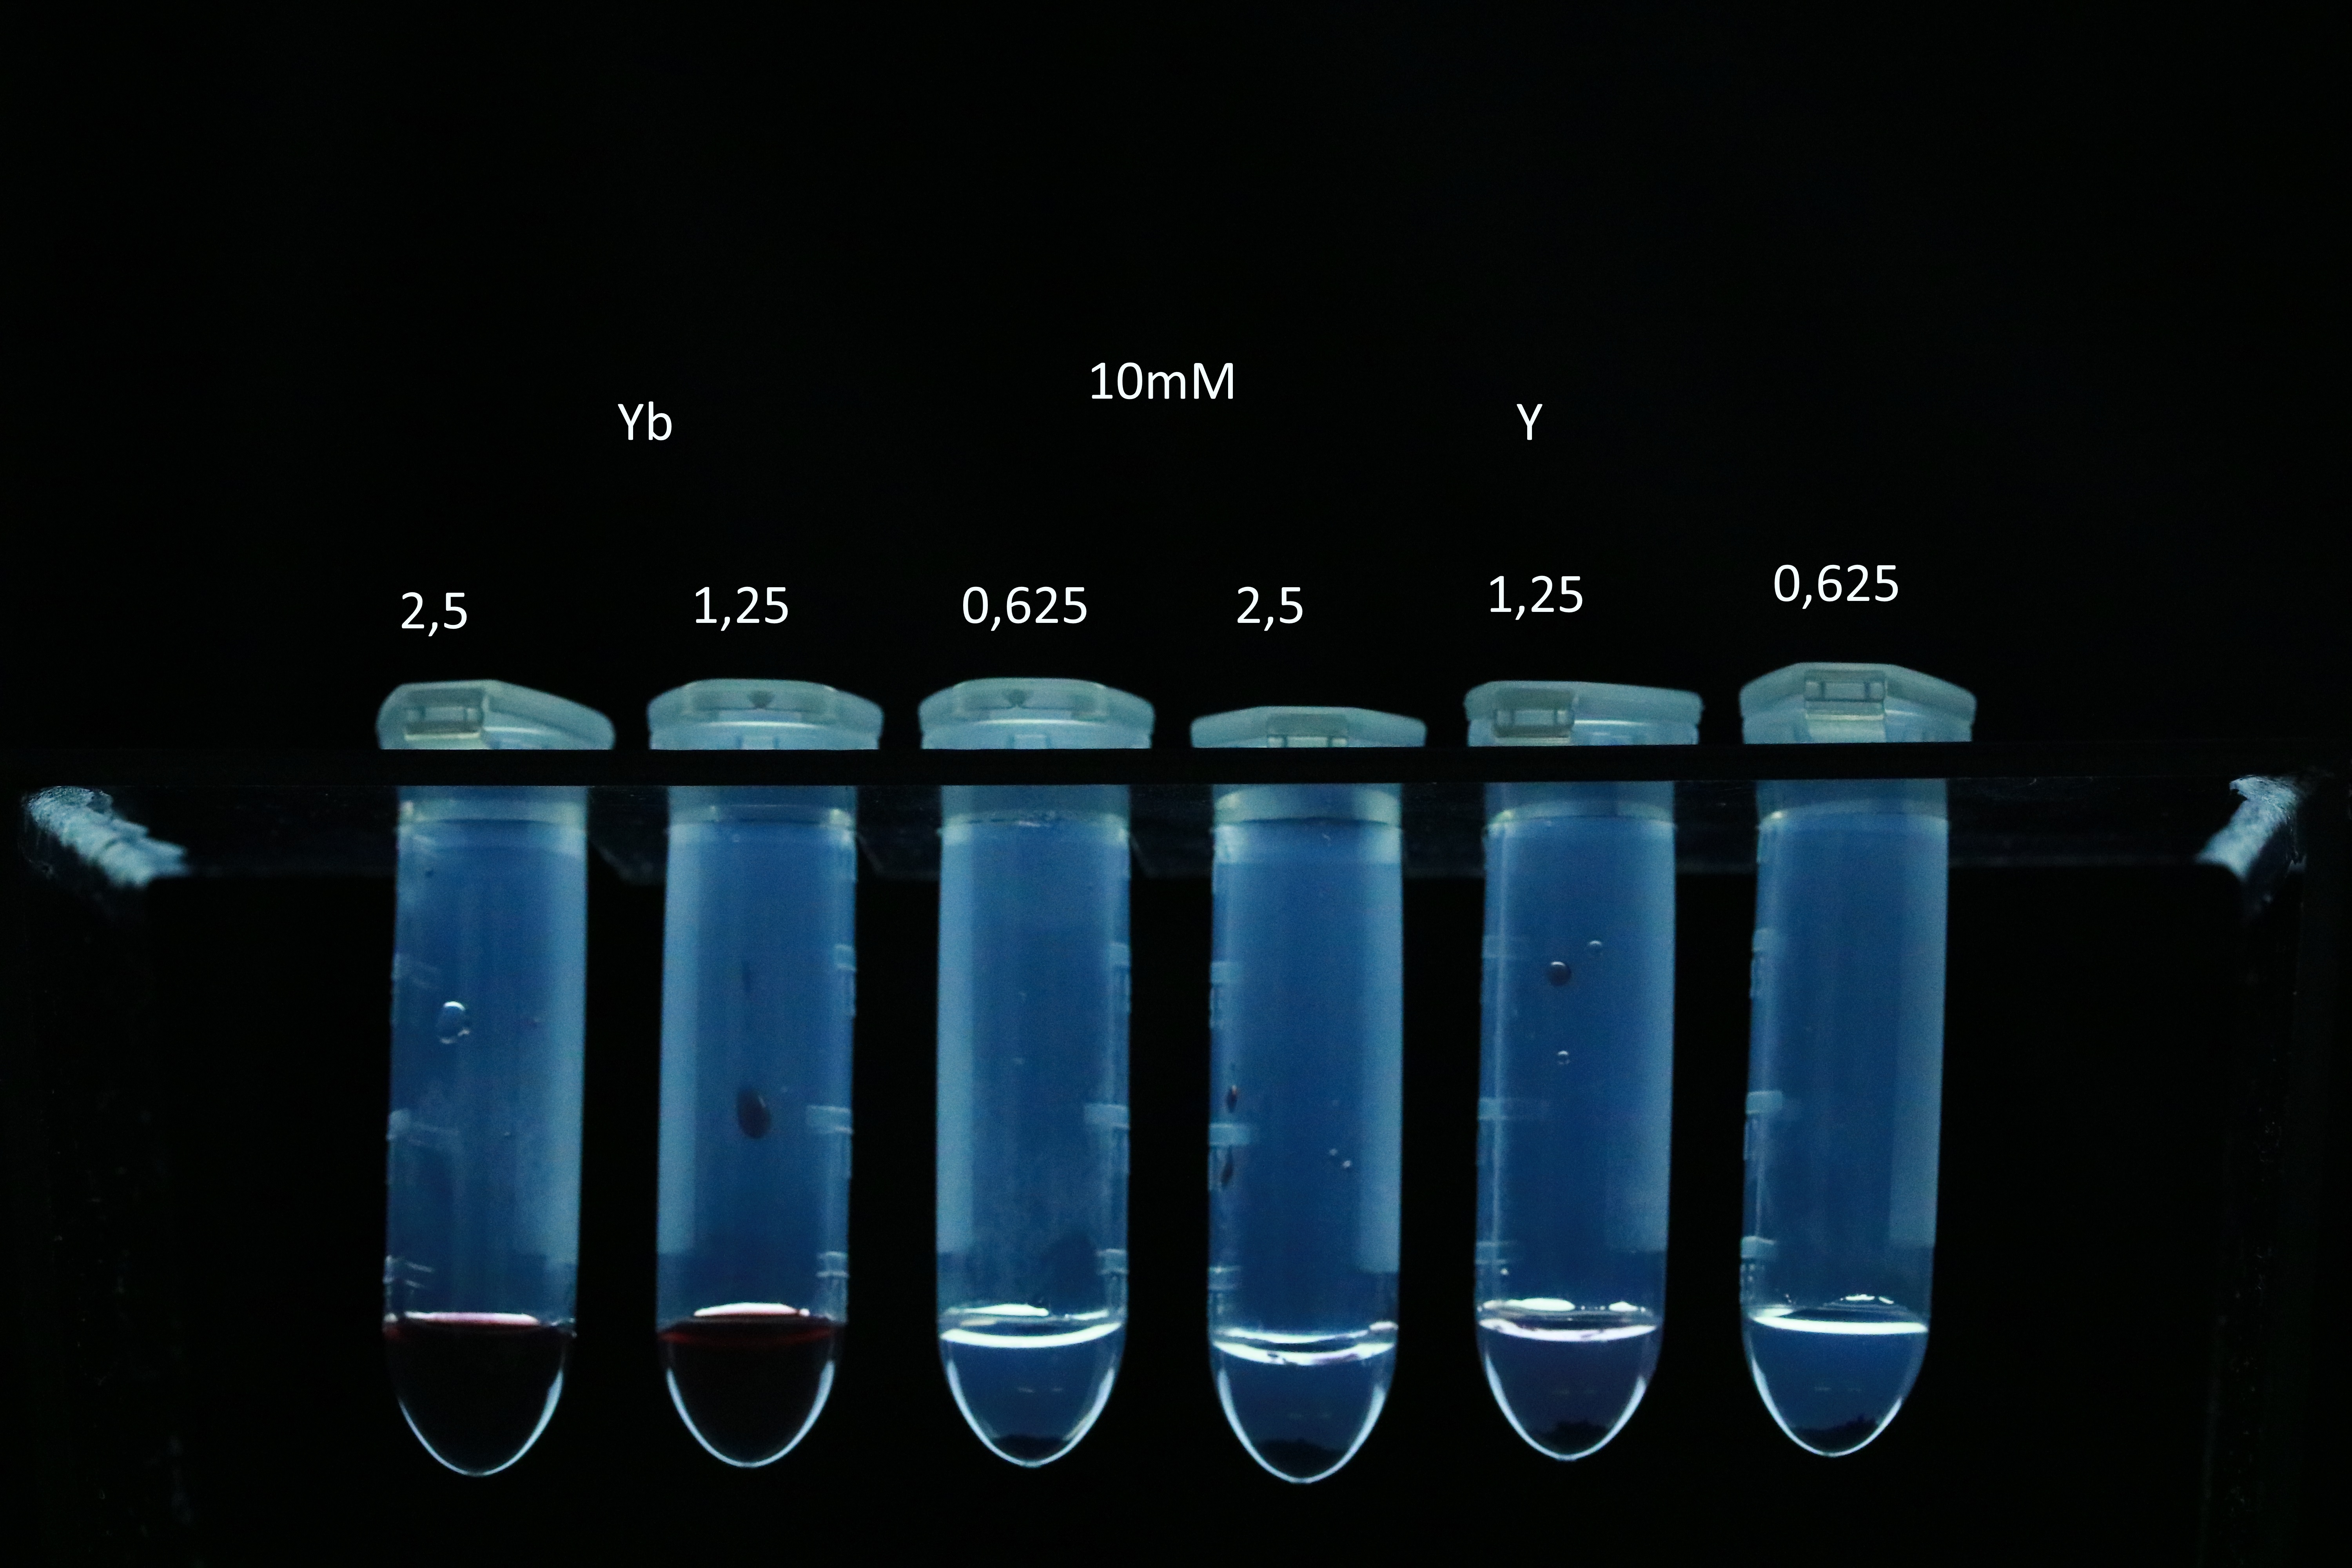
\includegraphics[width=0.6\textwidth]{Bilder/1Y-Yb-Gele} 	
			\caption{Übersicht der Gele mit 10 mM Yb$^{3+}$ und Y$^{3+}$-Lösung und 2,5; 1,25; 0,625 g/L Gold-NP-Lösung.}
			\label{fig:1Y-Yb-Gele}
		\end{figure}
		
		Da es bei den Proben mit Yttrium immer zu einer vollständigen Entfärbung kam, also sämtliches Gold aus der Lösung abgelagert wurde, wurde sich bei weiteren Untersuchungen auf diese beschränkt.
		Um festzustellen, ob es sich bei dem gebildeten Niederschlag um Gele handelte wurden TEM-Aufnahmen von einigen Proben vorgenommen.
		Dabei wurden jeweils die Extreme der verwendeten Konzentrationen näher untersucht.
		
		\begin{figure}[htbp]
			\centering
			\subfloat[\label{fig:Au-Y-}]{%
				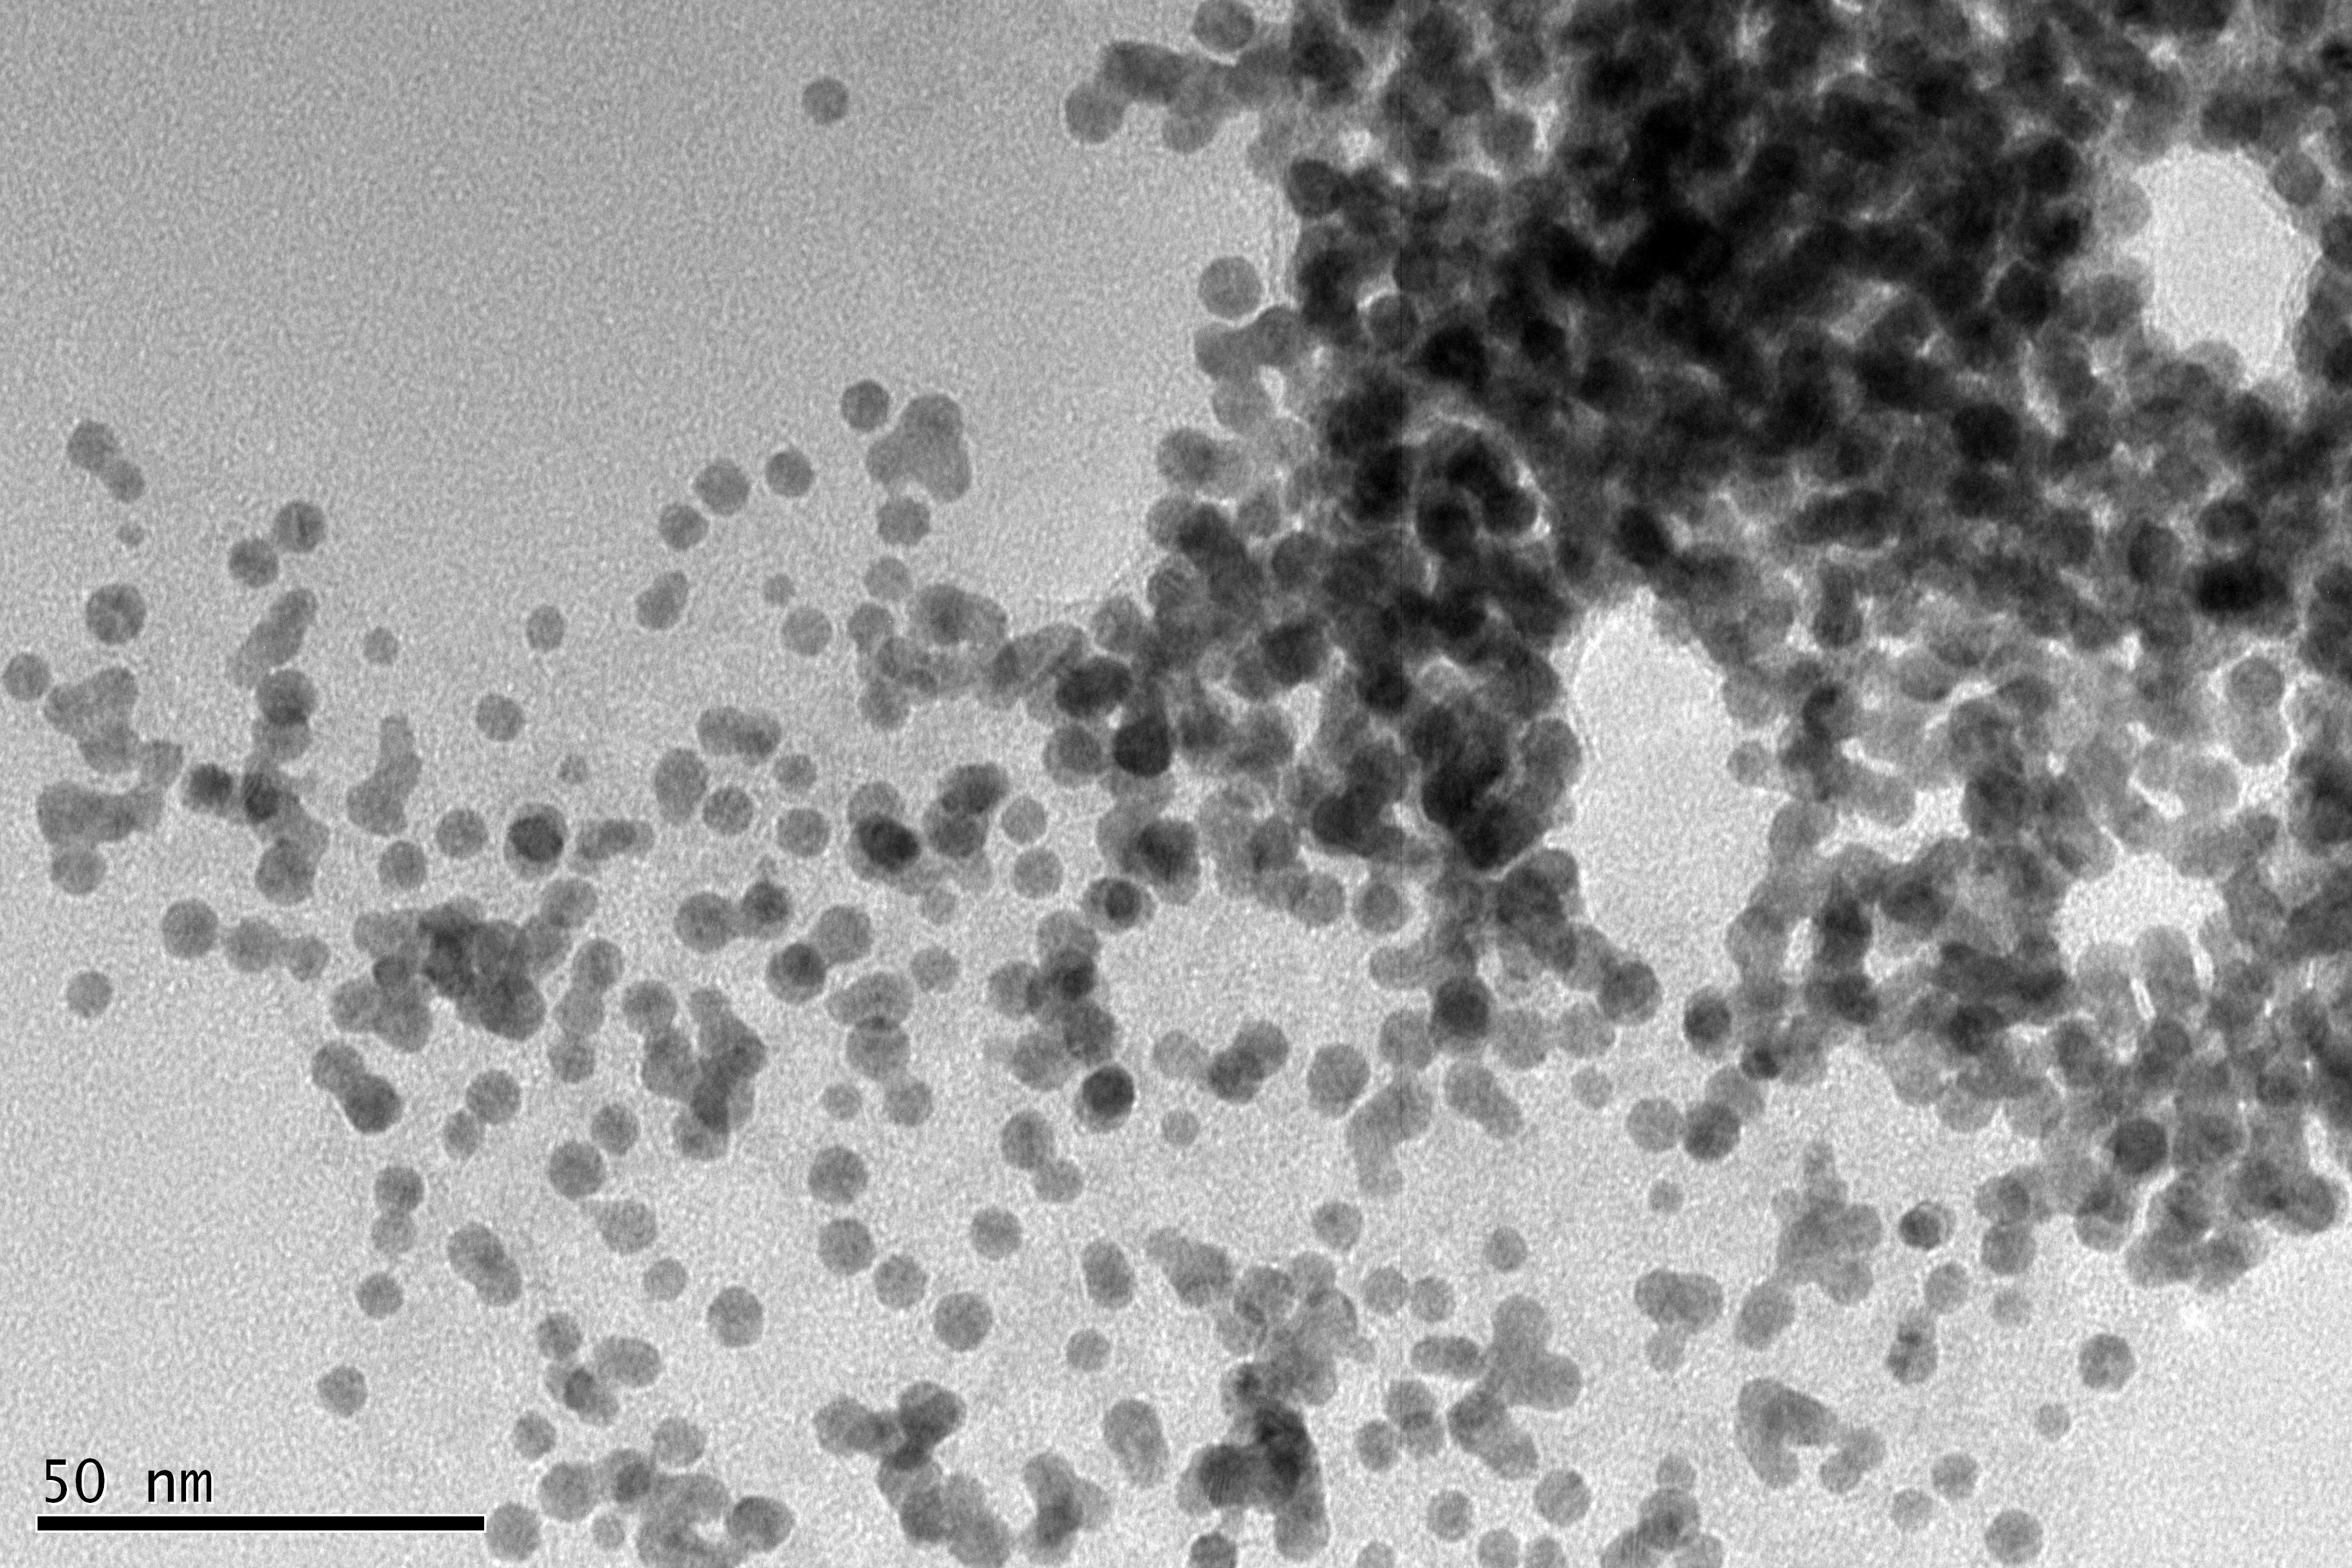
\includegraphics[width=0.45\linewidth]{Bilder/Au-Y-}}
			\subfloat[\label{fig:Au+Y-}]{%
				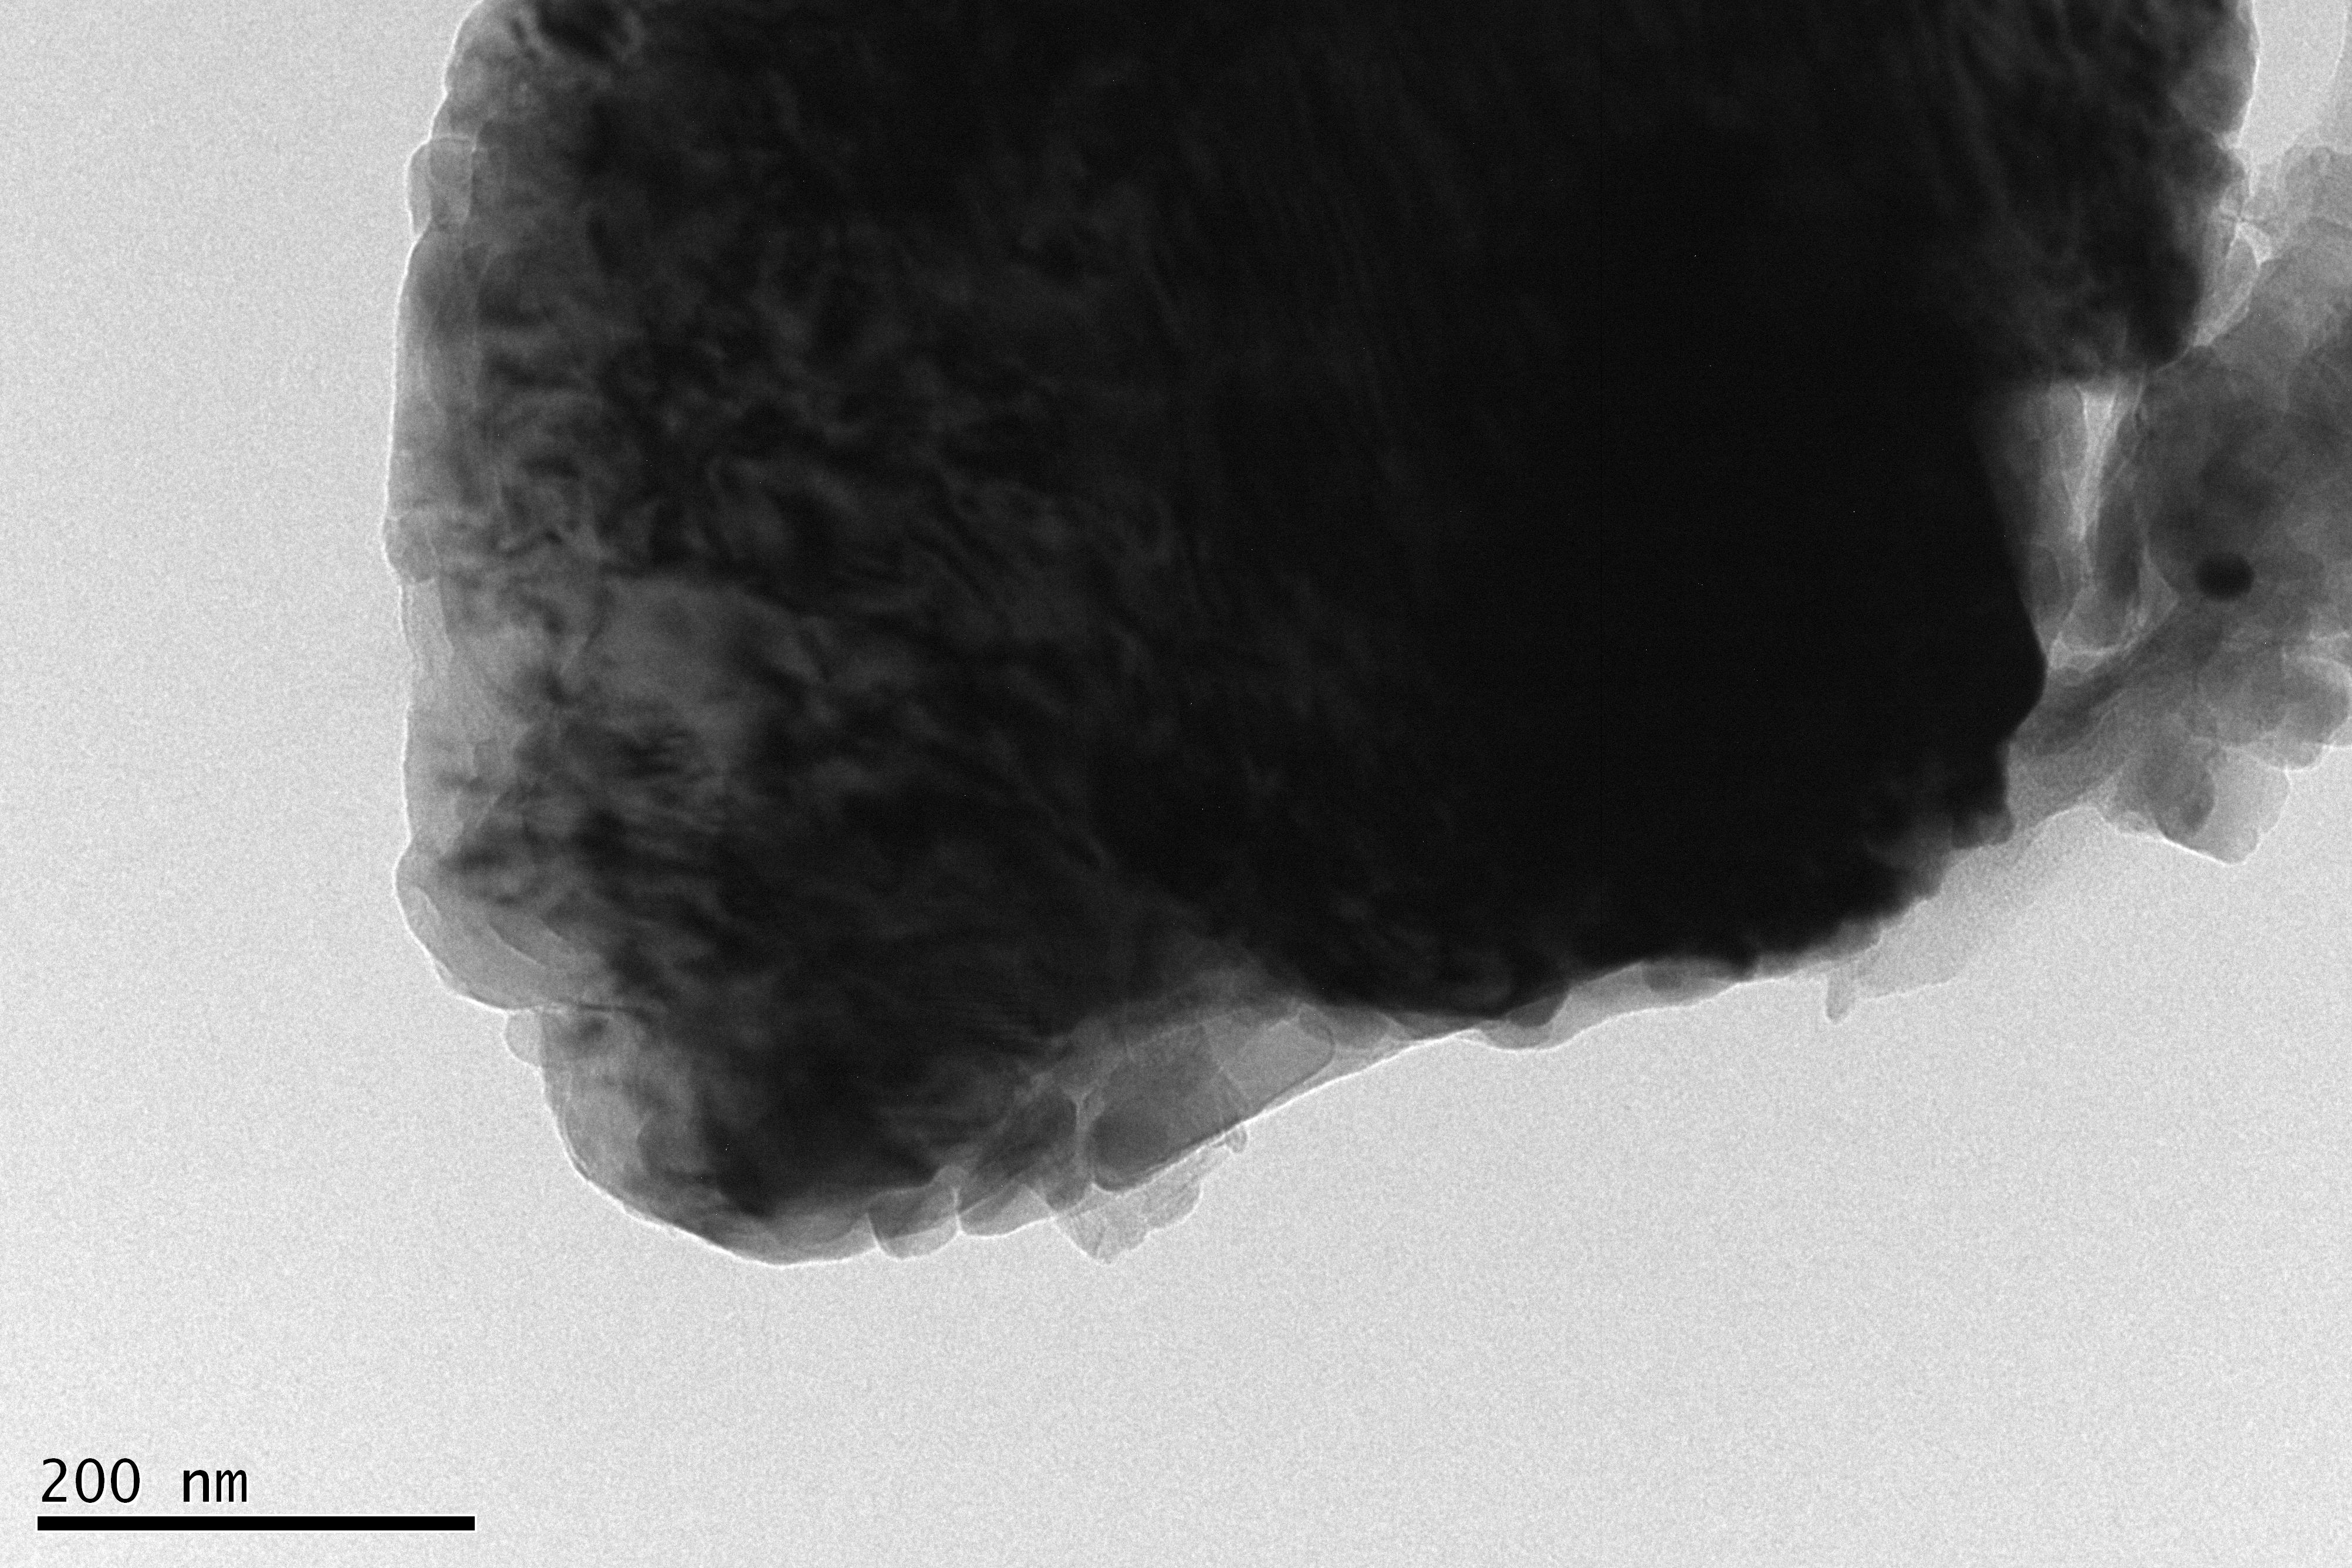
\includegraphics[width=0.45\linewidth]{Bilder/Au+Y-}}\\
			\subfloat[\label{fig:Au-Y+}]{%
				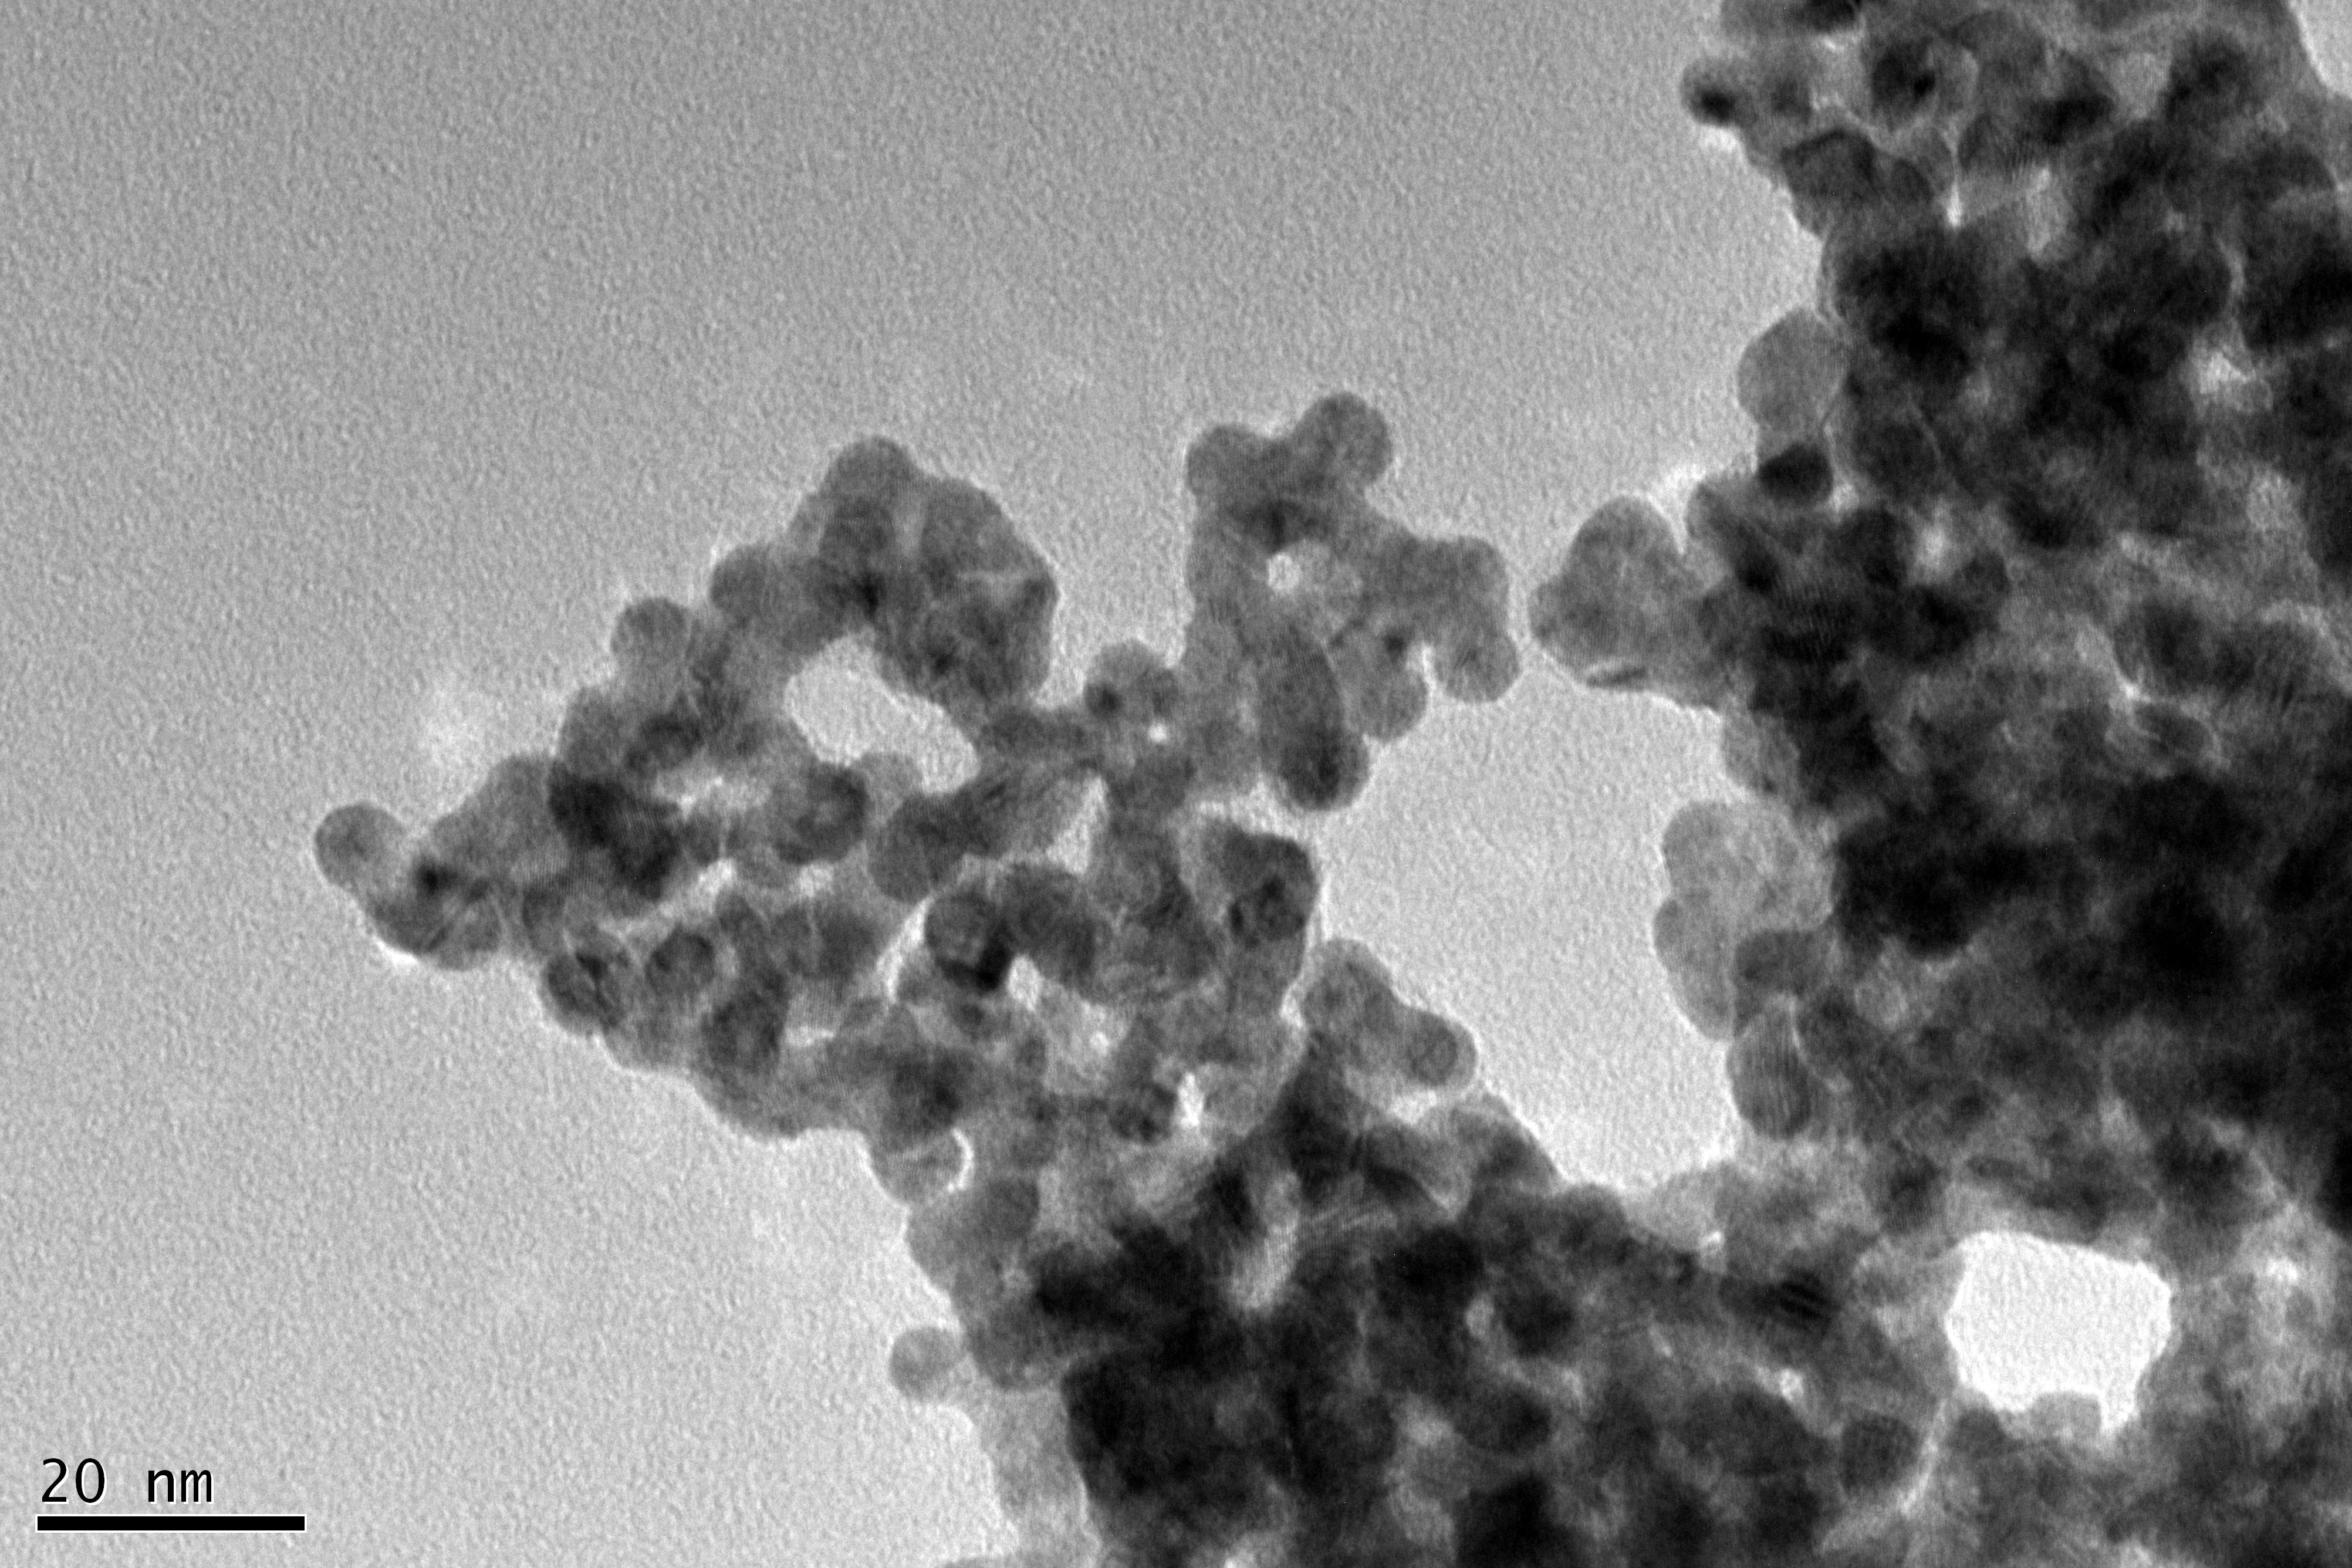
\includegraphics[width=0.45\linewidth]{Bilder/Au-Y+}}
			\subfloat[\label{fig:Au+Y+}]{%
				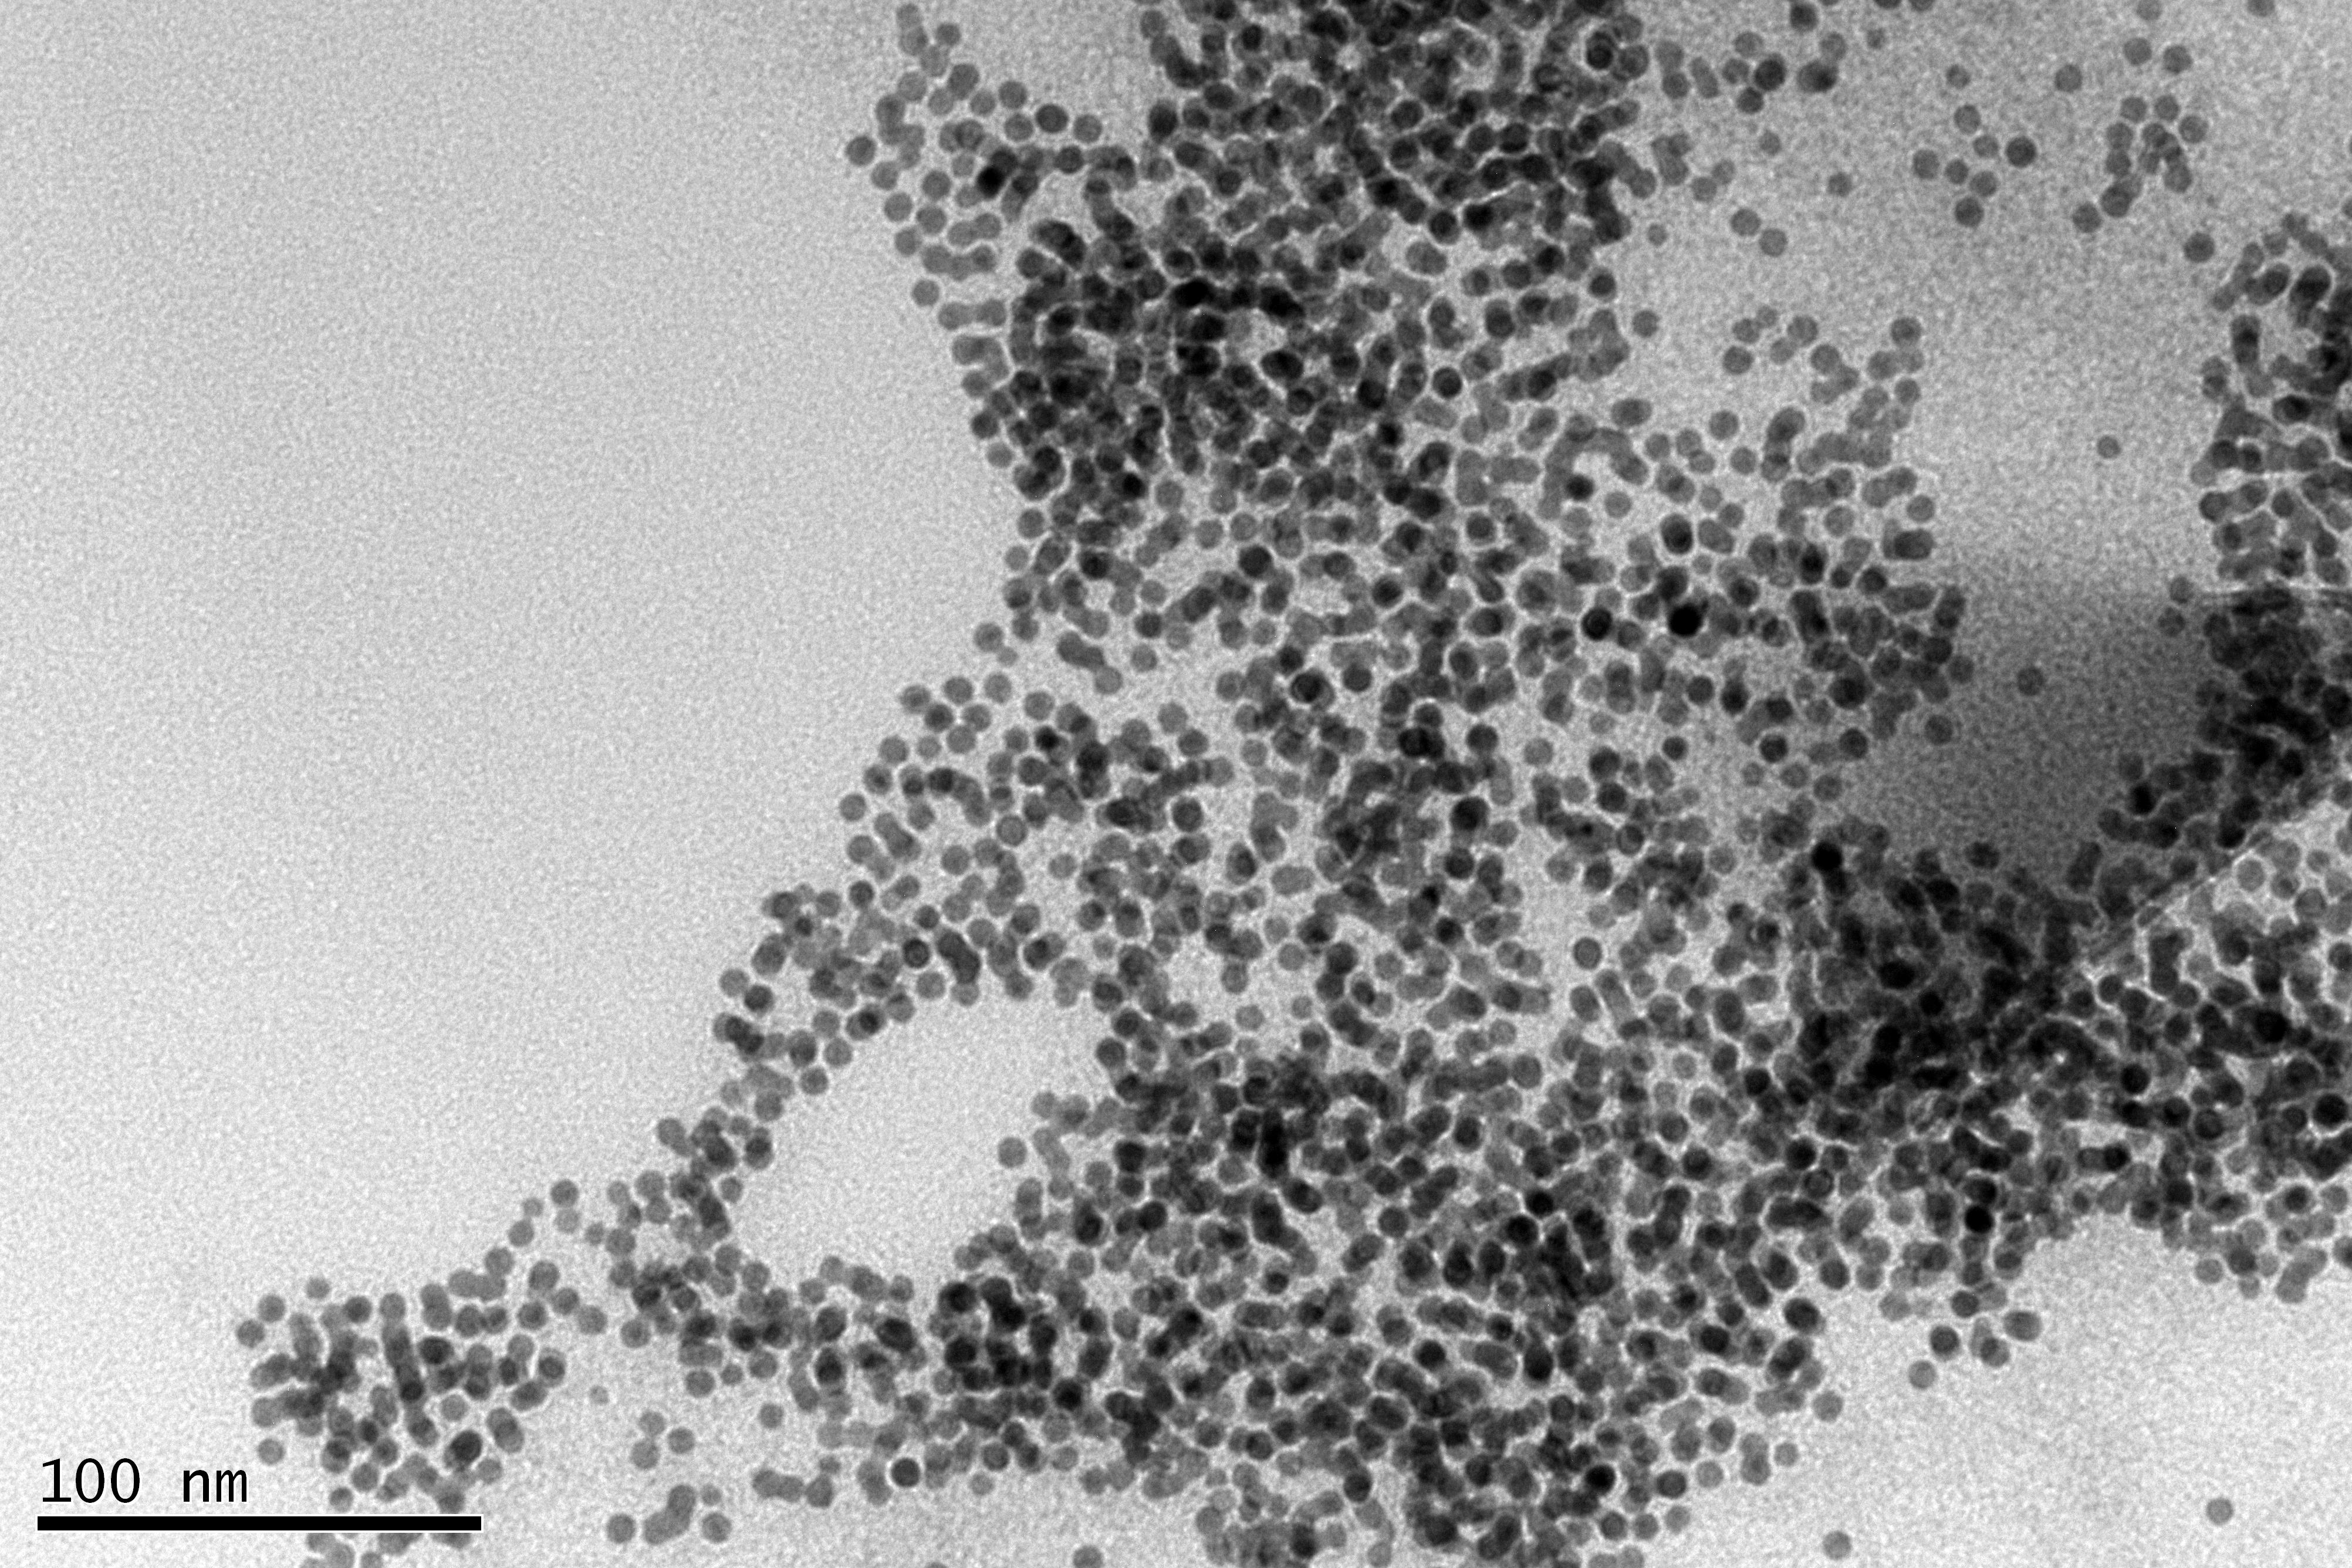
\includegraphics[width=0.45\linewidth]{Bilder/Au+Y+}}
			\caption{TEM-Bilder nach Zugabe von Yttriumchlorid mit den Konzentrationen: \emph{(a)}:~Au:~\SI{0,625}{\gram\per\liter}, Y: 1~mM;
			\emph{(b)}:~Au:~\SI{2,5}{\gram\per\liter}, Y: 1~mM
			\emph{(c)}:~Au:~\SI{0,625}{\gram\per\liter}, Y: 10~mM
			\emph{(d)}:~Au:~\SI{2,5}{\gram\per\liter}, Y: 10~mM} 
			\label{fig:Y-Gele}
		\end{figure}
		
		Die TEM-Bilder zeigen, dass es zu deutlichen Unterschieden bei den verschiedenen Konzentrationen kommt.
		So entstehen bei hoher Goldkonzentration und niedriger Yttriumkonzentration keine Gele sondern es entsteht einfach ein großer Klumpen (\cref{fig:Au+Y-}).
		Bei hoher Goldkonzentration und hoher Yttriumkonzentration hingegen liegen die Partikel alle seperat voneinander vor und es wurde also auch hier kein Gel gebildet(\cref{fig:Au+Y+}). 
		Bei den Versuchen mit den geringen Goldkonzentrationen konnte bei beiden Yttriumkonzentration eine Anlagerung der Gold-NP aneinander beobachtet werden.
		Bei geringer Yttriumkonzentration lagen jedoch ein größerer Teil der Partikel einzeln vor wie \cref{fig:Au-Y-} zeigt. 
		Das, was dem Aussehen klassischer Nanopartikelgele am nächsten kam war die Probe mit niedriger Goldkonzentration und höherer Yttriumkonzentration (\cref{fig:Au-Y+}). 
		Hier sind die Partikel miteinander venetzt und bildeten dabei Hohlräume.
		
		
		
	 
	
	
	\subsubsection{Untersuchung von citratstabilisierten Gelen}
		
		Die für die Gelierung hergestellten Silber- und Goldpartikeln wurden per UV-vis-Absorptionsspektroskopie untersucht.
		Sie zeigten typische Absorptionsmaxima bei $\lambda_{Gold}$=\SI{525}{\nano\meter} und $\lambda_{Silber}$=\SI{412}{\nano\meter}, wie \cref{fig:Abs-cit} zeigt.
		\begin{figure}[H]
			\centering
			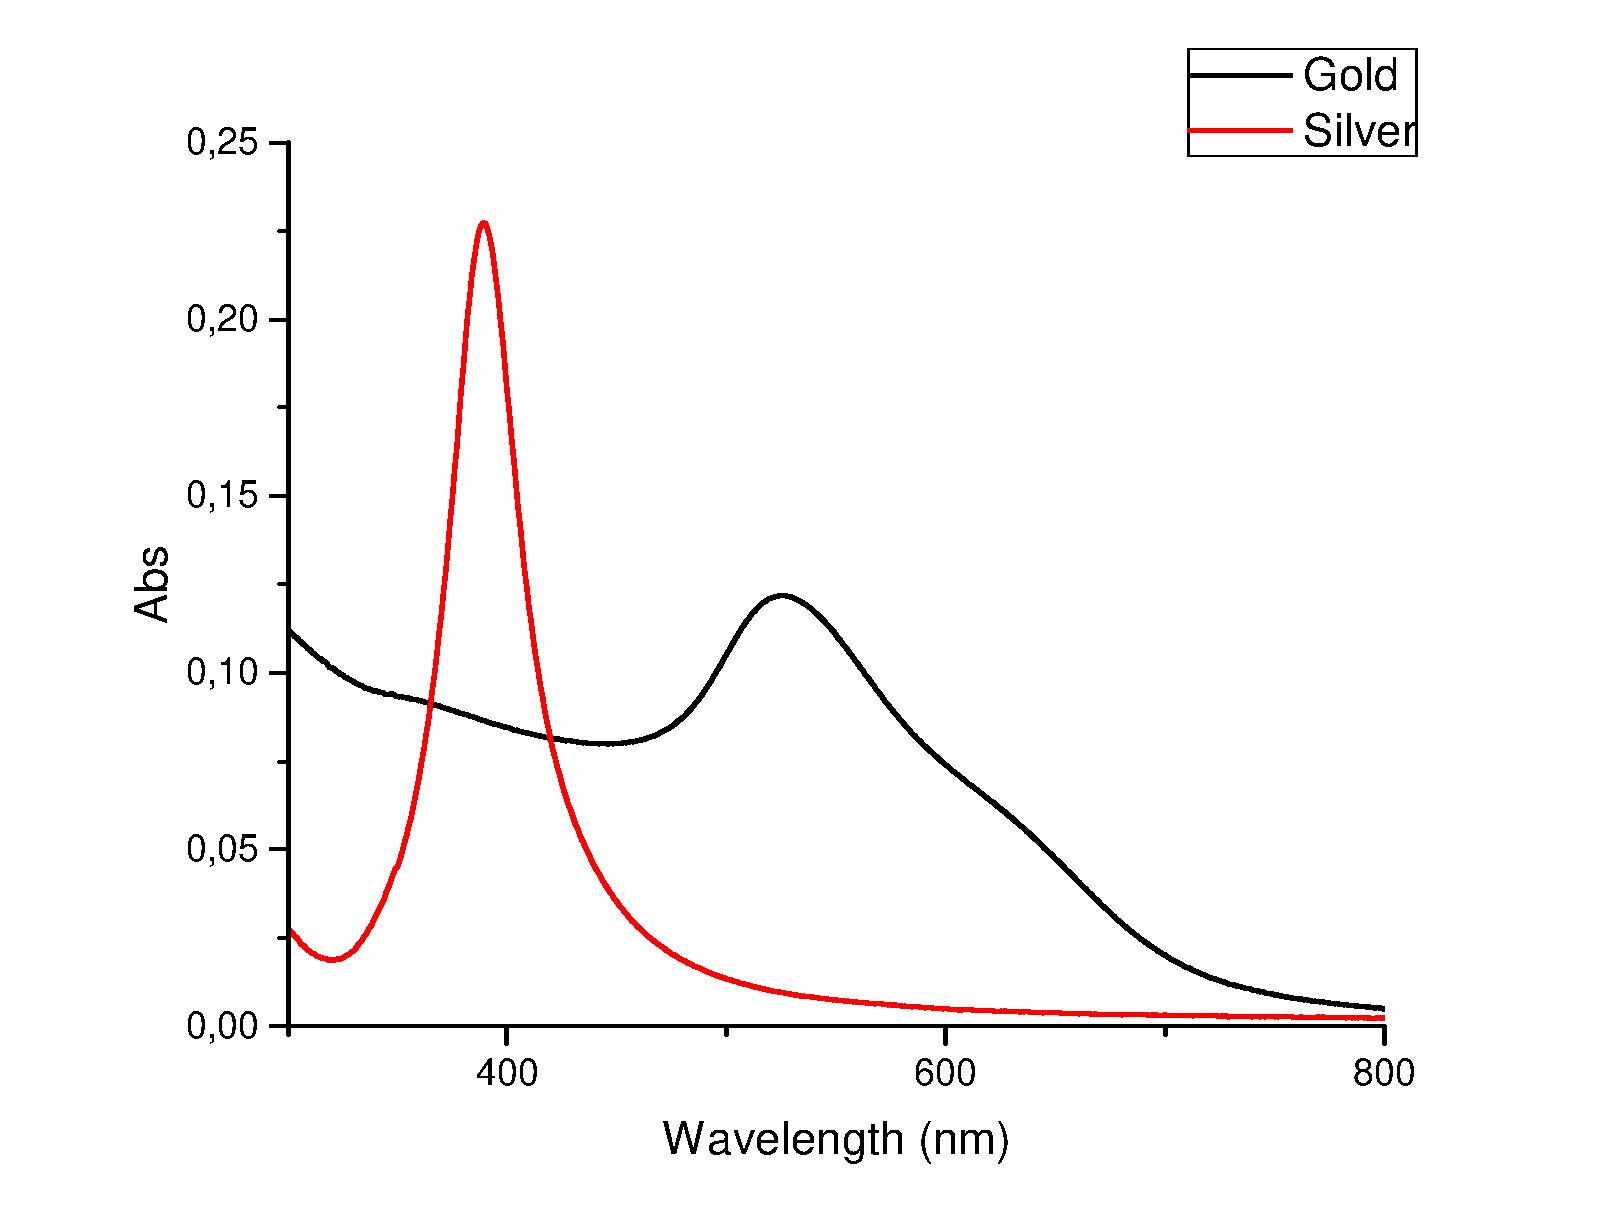
\includegraphics[width=0.6\textwidth]{Bilder/Citrat-NP} 	
			\caption{UV-vis-Absorptionsspektren von Gold-NP und Silber-NP.}
			\label{fig:Abs-cit}
		\end{figure}
	
		Da bei den Versuchen mit reinem Gold und Silber keine festen Gele entstanden sind wurden diese auch nicht weiter untersucht.
		Im Vergleich zu den Hydrogelen, ist das Gel während des Austausches der flüssigen Phase zu TOP zu etwa ein Drittel des Ausgangsvolumen zusammengeschrumpft.
		Von den bimetallischen Gelen aus Gold- und Silbernanopartikeln wurden TEM-Bilder nach dem Phasentransfer in TOP aufgenommen.
		Es ist ein Netzwerk zu erkennen, dass aus kleinen Partikeln ($\approx$~\SI{10}{\nano\meter}), die miteinander Verknüpft sind und dabei viele große Zwischenräume besitzt, wie \cref{fig:Gel-C} zeigt. 
		
		\begin{figure}[htbp]
			\centering
			\subfloat[\label{fig:Gel-C-1}]{%
				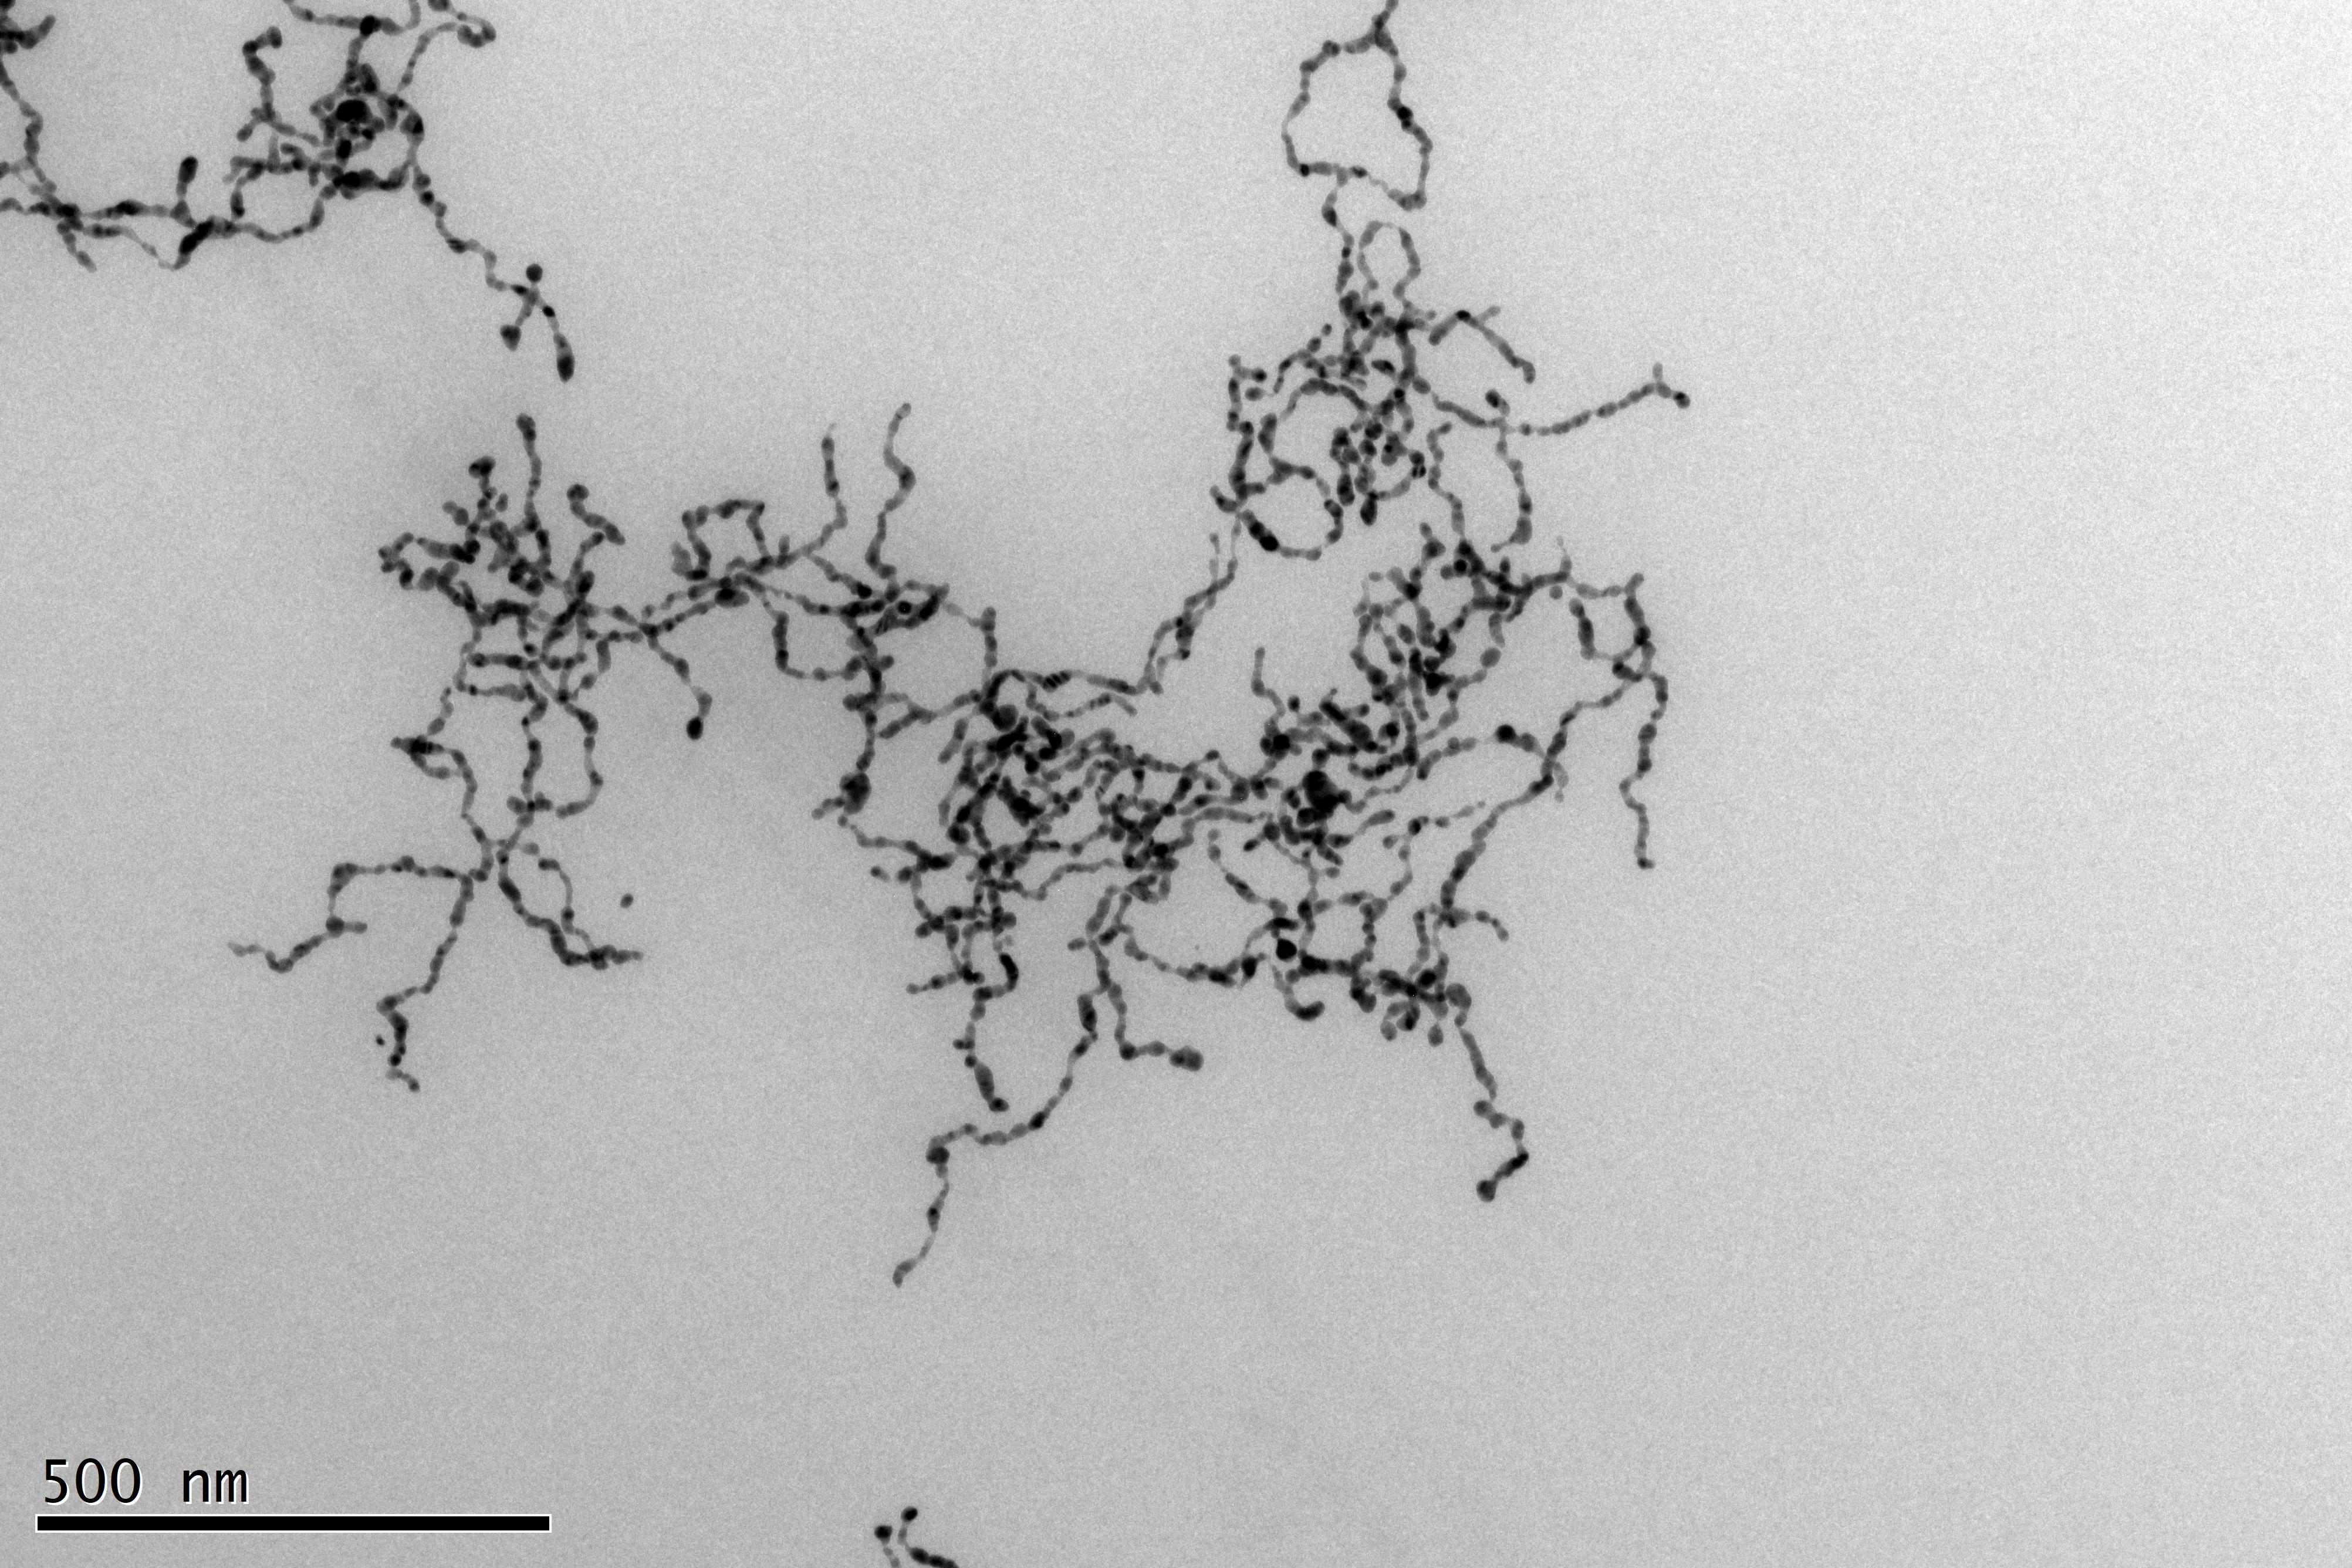
\includegraphics[width=0.33\linewidth]{Bilder/Gel-C-1}}
			\subfloat[\label{fig:Gel-C-2}]{%
				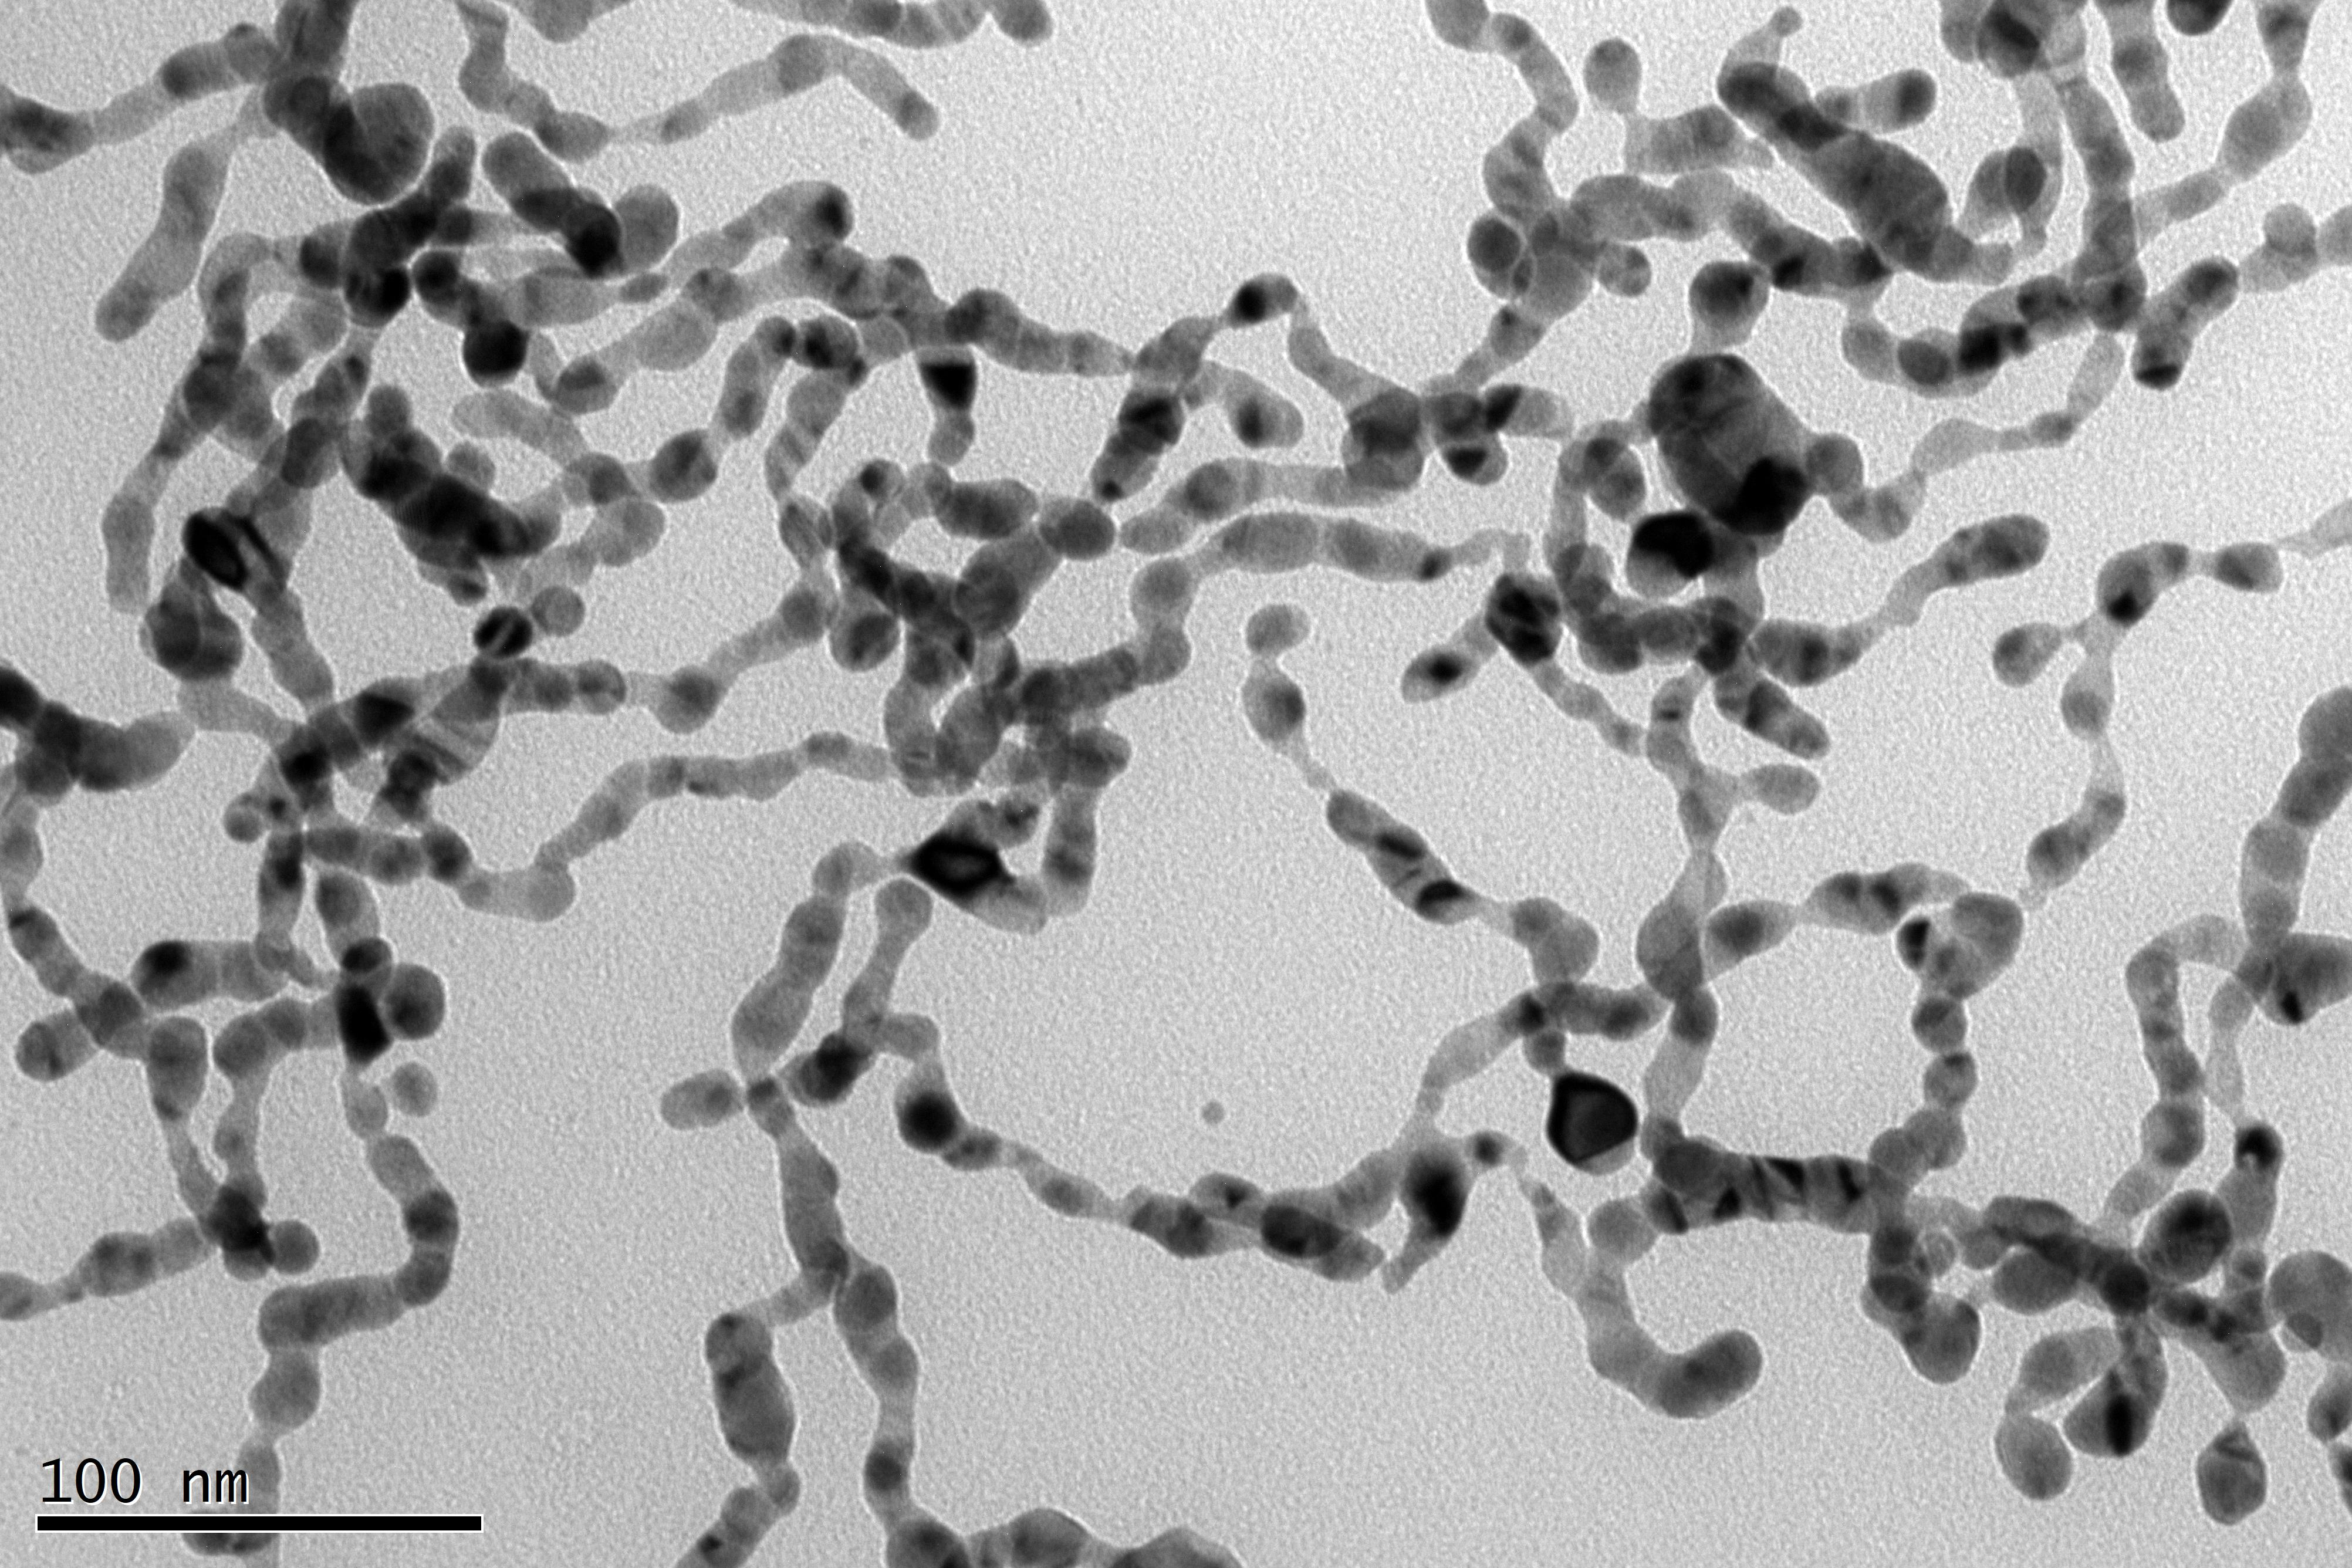
\includegraphics[width=0.33\linewidth]{Bilder/Gel-C-2}}
			\subfloat[\label{fig:Gel-C-3}]{%
				\includegraphics[width=0.33\linewidth]{Bilder/gel-C-3}}
			\caption{TEM-Bilder der citratstrabilisierten Gele in TOP}
			\label{fig:Gel-C}
		\end{figure}
		
	\subsubsection{Untersuchung der Gele aus ethanolischem Ansatz}
		
		Da bei diesen Gelen der Schritt der Nukleation und der Schritt der Gelierung nicht separat voneinander Ablaufen, war ein groberes, weniger gleichmäßiges Gel als bei den citratstabilisierten zu erwarten.
		Dies war auch wie \cref{fig:Gel-C} zeigt der Fall.
		Insgesamt zeigt das Gel weniger Zwischenräume bei einem deutlich größeren Partikeldurchmesser ($\approx$~\SI{100}{\nano\meter}).
		
		\begin{figure}[htbp]
			\centering
			\subfloat[\label{fig:Gel-E-1}]{%
				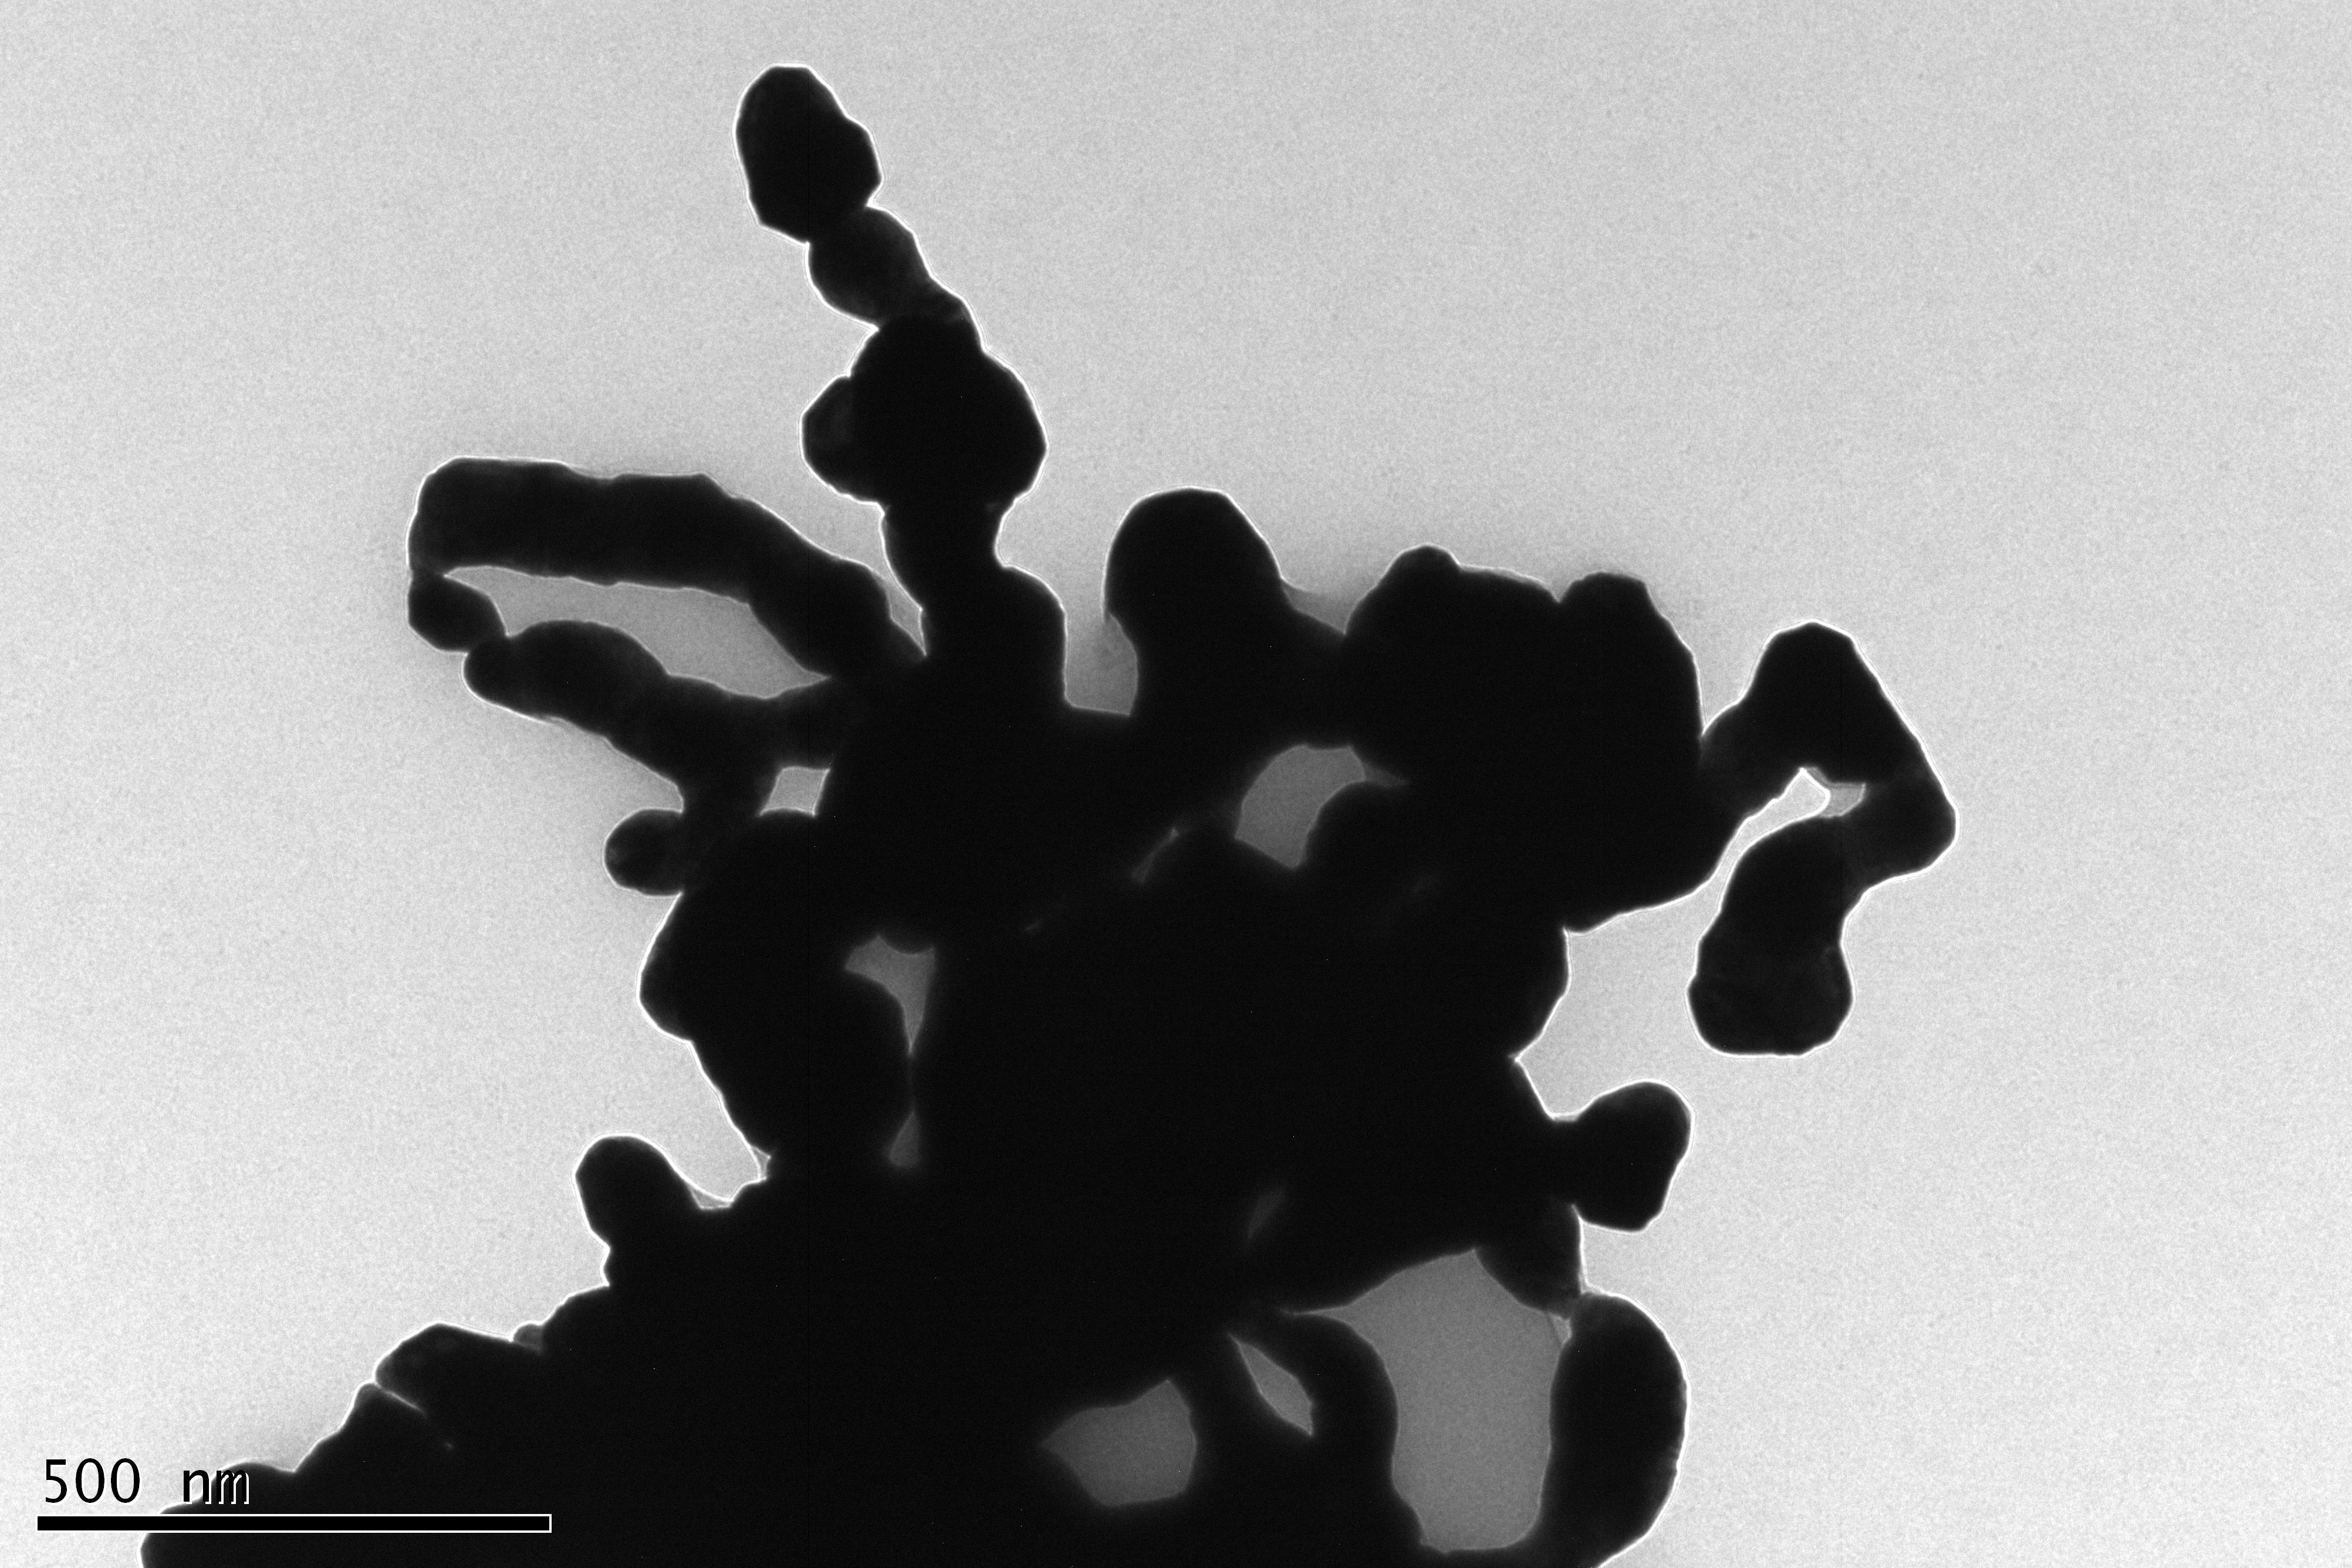
\includegraphics[width=0.45\linewidth]{Bilder/Gel-E-1}}
			\subfloat[\label{fig:Gel-E-2}]{%
				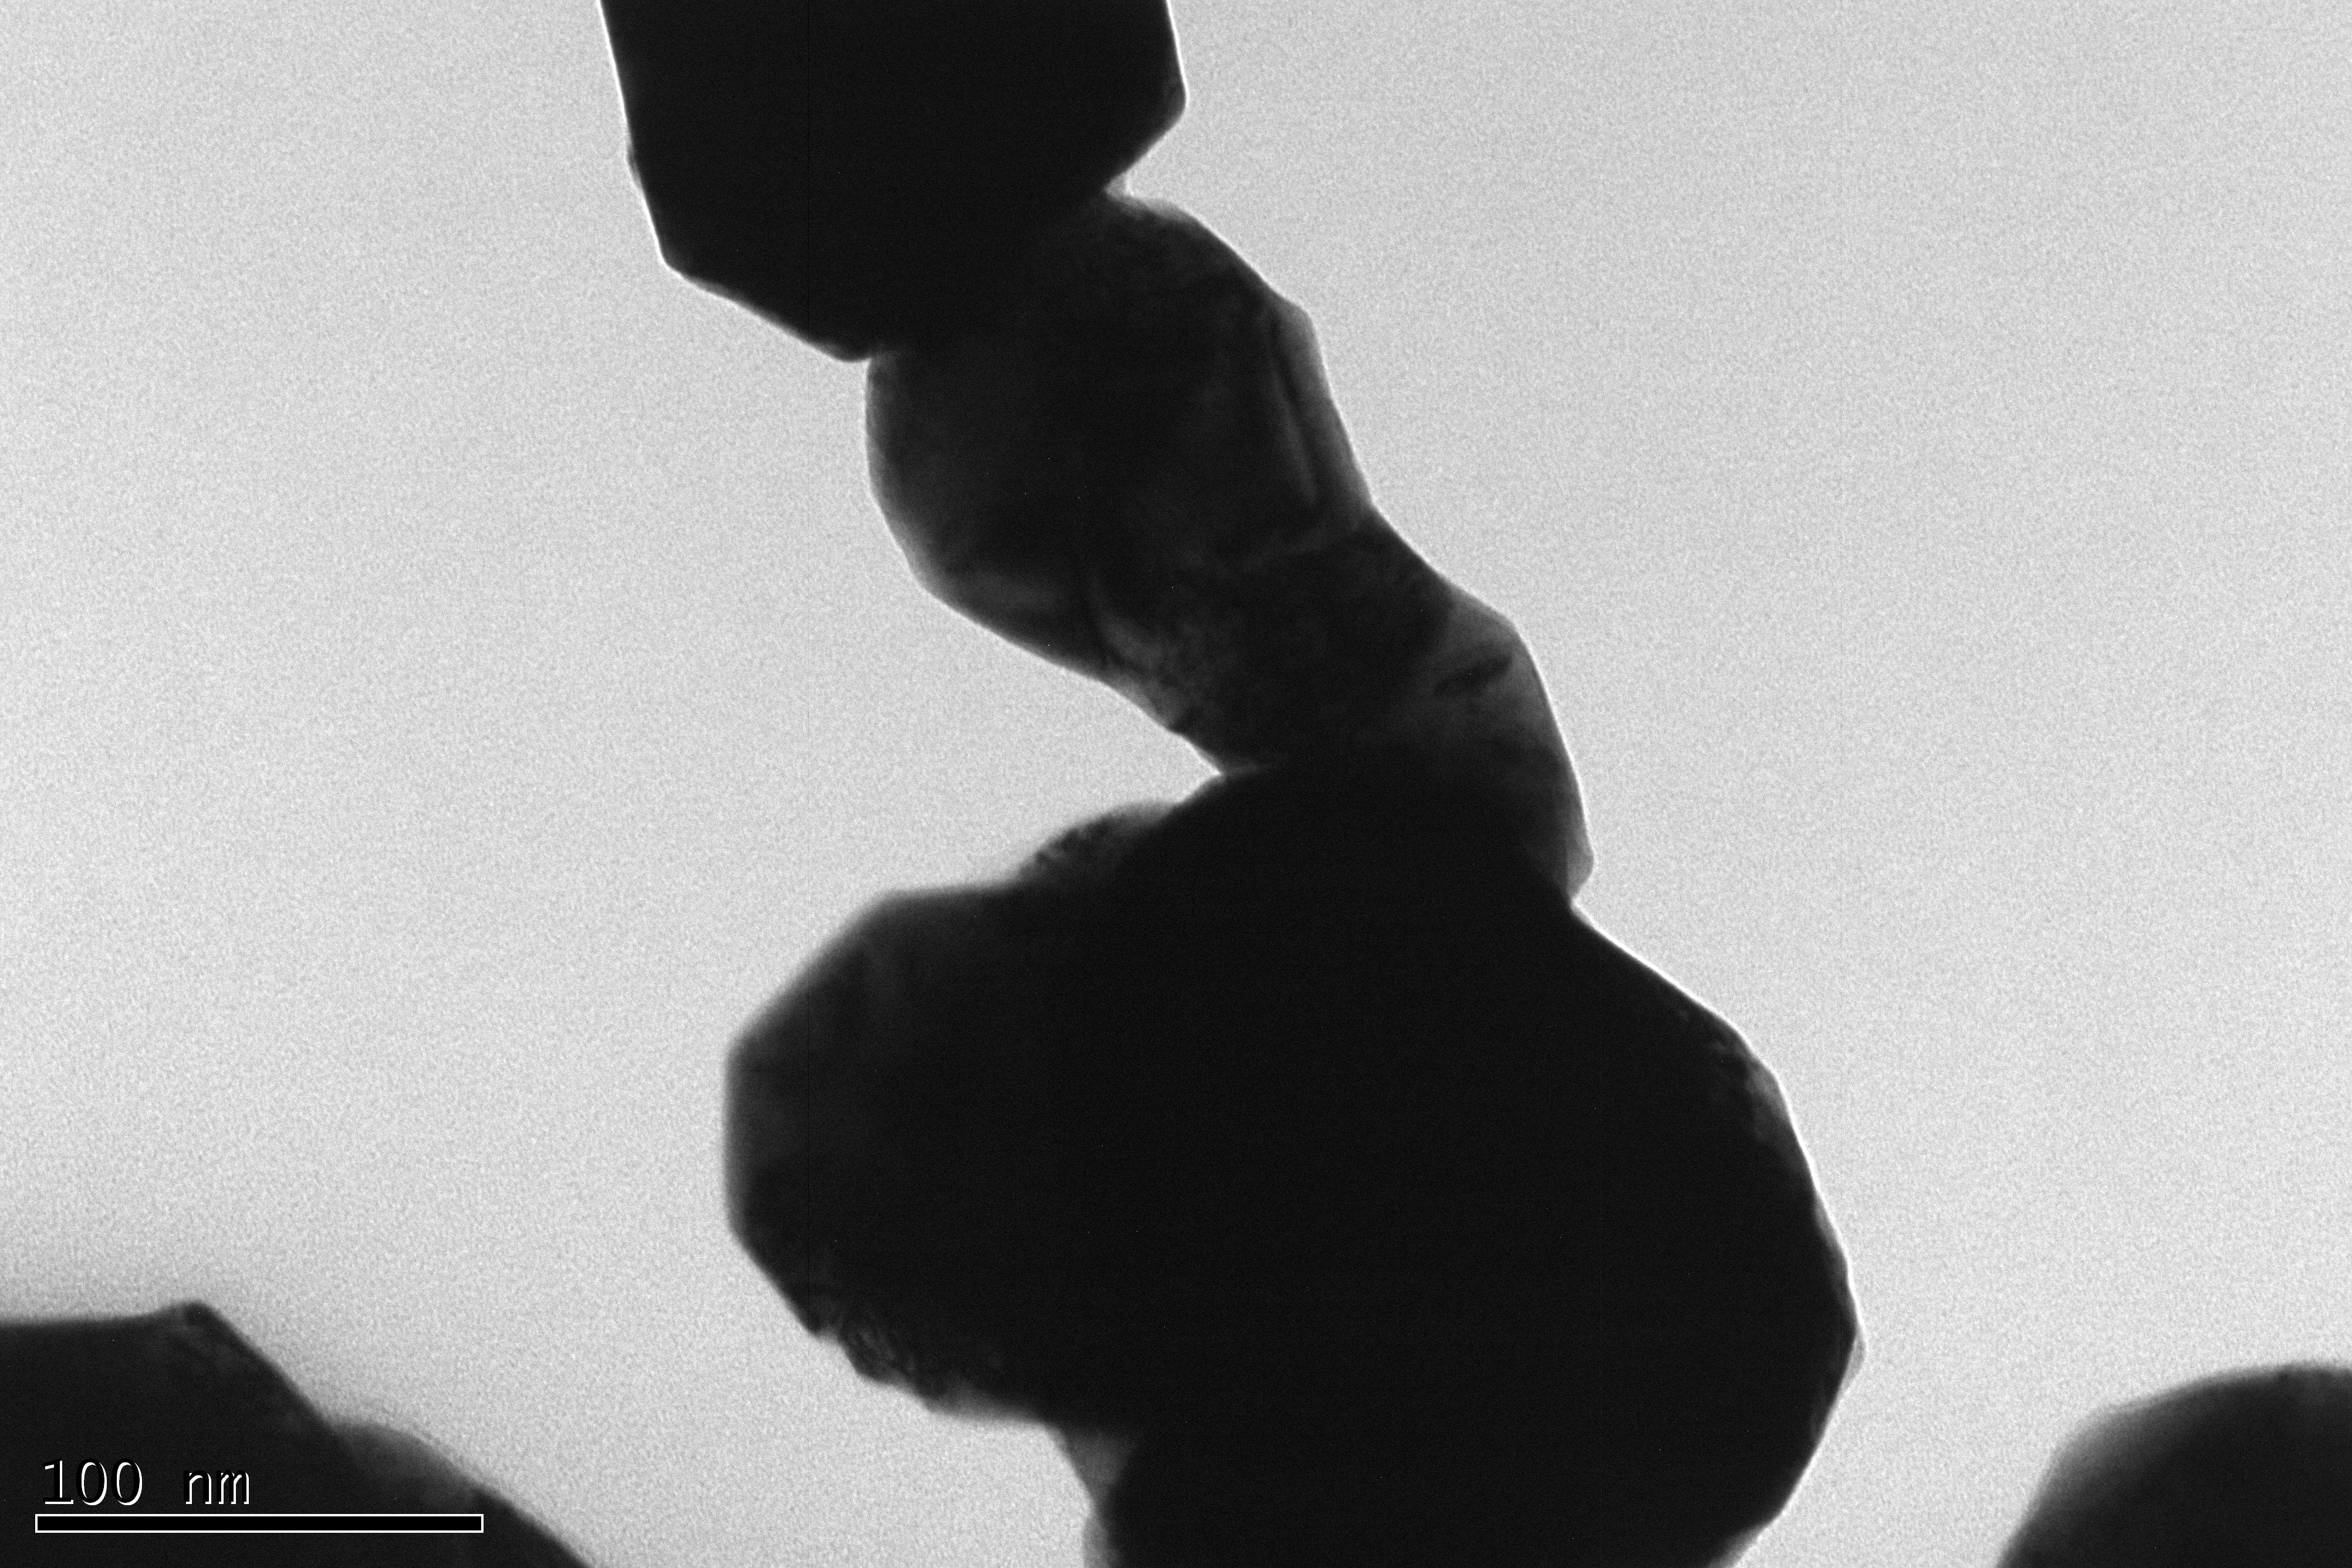
\includegraphics[width=0.45\linewidth]{Bilder/Gel-E-2}}
			\caption{TEM Bilder der Gele aus ethanolischem Ansatz}
			\label{fig:Gel-E}
		\end{figure}
	
	\subsection{Untersuchung der Metallsulfidsynthese in Anwesenheit von Gelen}
	
	Nachdem die Proben mit Goldpartikeln zeigten, dass bei der thermischen Zersetzung von \ch{Cu[DDTC]2} sich CuS nicht nur getrennt vom Gold bildet, wurde hier getestet ob sich CuS (und später auch CdS und ZnS) an schon vorhandene Gele anlagert bzw. anwächst und mit welchen Parametern man dieses Verhalten beeinflussen kann.
	Dabei wurde hauptsächlich mit den Gelen aus ethanolischem Ansatz gearbeitet.
	
	Es zeigt sich direkt, dass wie zu erwarten die Gele zusammenschrumpfen, während des Verdampfungsprozesses.
	Allerdings sind diese Xerogele, wie man in \cref{fig:vn} nicht so stark geschrumpft, wie es von anderen Gelen bekannt ist, was mit der relativ groben Struktur der Gele und verhältnismäßig kleinen Zwischenräumen, die kollabieren können, zusammenhängt.
	
	
	\begin{figure}[H]
	\centering
	\subfloat[\label{fig:vorher}]{%
		\includegraphics[width=0.45\linewidth]{Bilder/Gel-E-vorher}}
	\subfloat[\label{fig:nachher}]{%
		\includegraphics[width=0.45\linewidth]{Bilder/Gel-E-nachher}}
	\caption{Vergleich der Gele \emph{(a)}: vor und \emph{(b)}: nach der Erhitzung}
	\label{fig:vn}
	\end{figure} 


	Die TEM-Aufnahmen des Gels, das mit \ch{Cu[DDTC]2} bei \SI{290}{\degreeCelsius} bearbeitet wurde, die in \cref{fig:E-Cu} gezeigt sind, zeigt, dass sich CuS am Gel gebildet hat.
	Von einer kompletten Schale ist es noch weit entfernt, aber zeigt, dass es möglich ist, mittels  thermischer Zersetzung von \ch{Cu[DDTC]2} das daraus entstehende CuS daran anzulagern.
	
	\begin{figure}[H]
		\centering
		\subfloat[\label{fig:Gel-E-Cu_1}]{%
			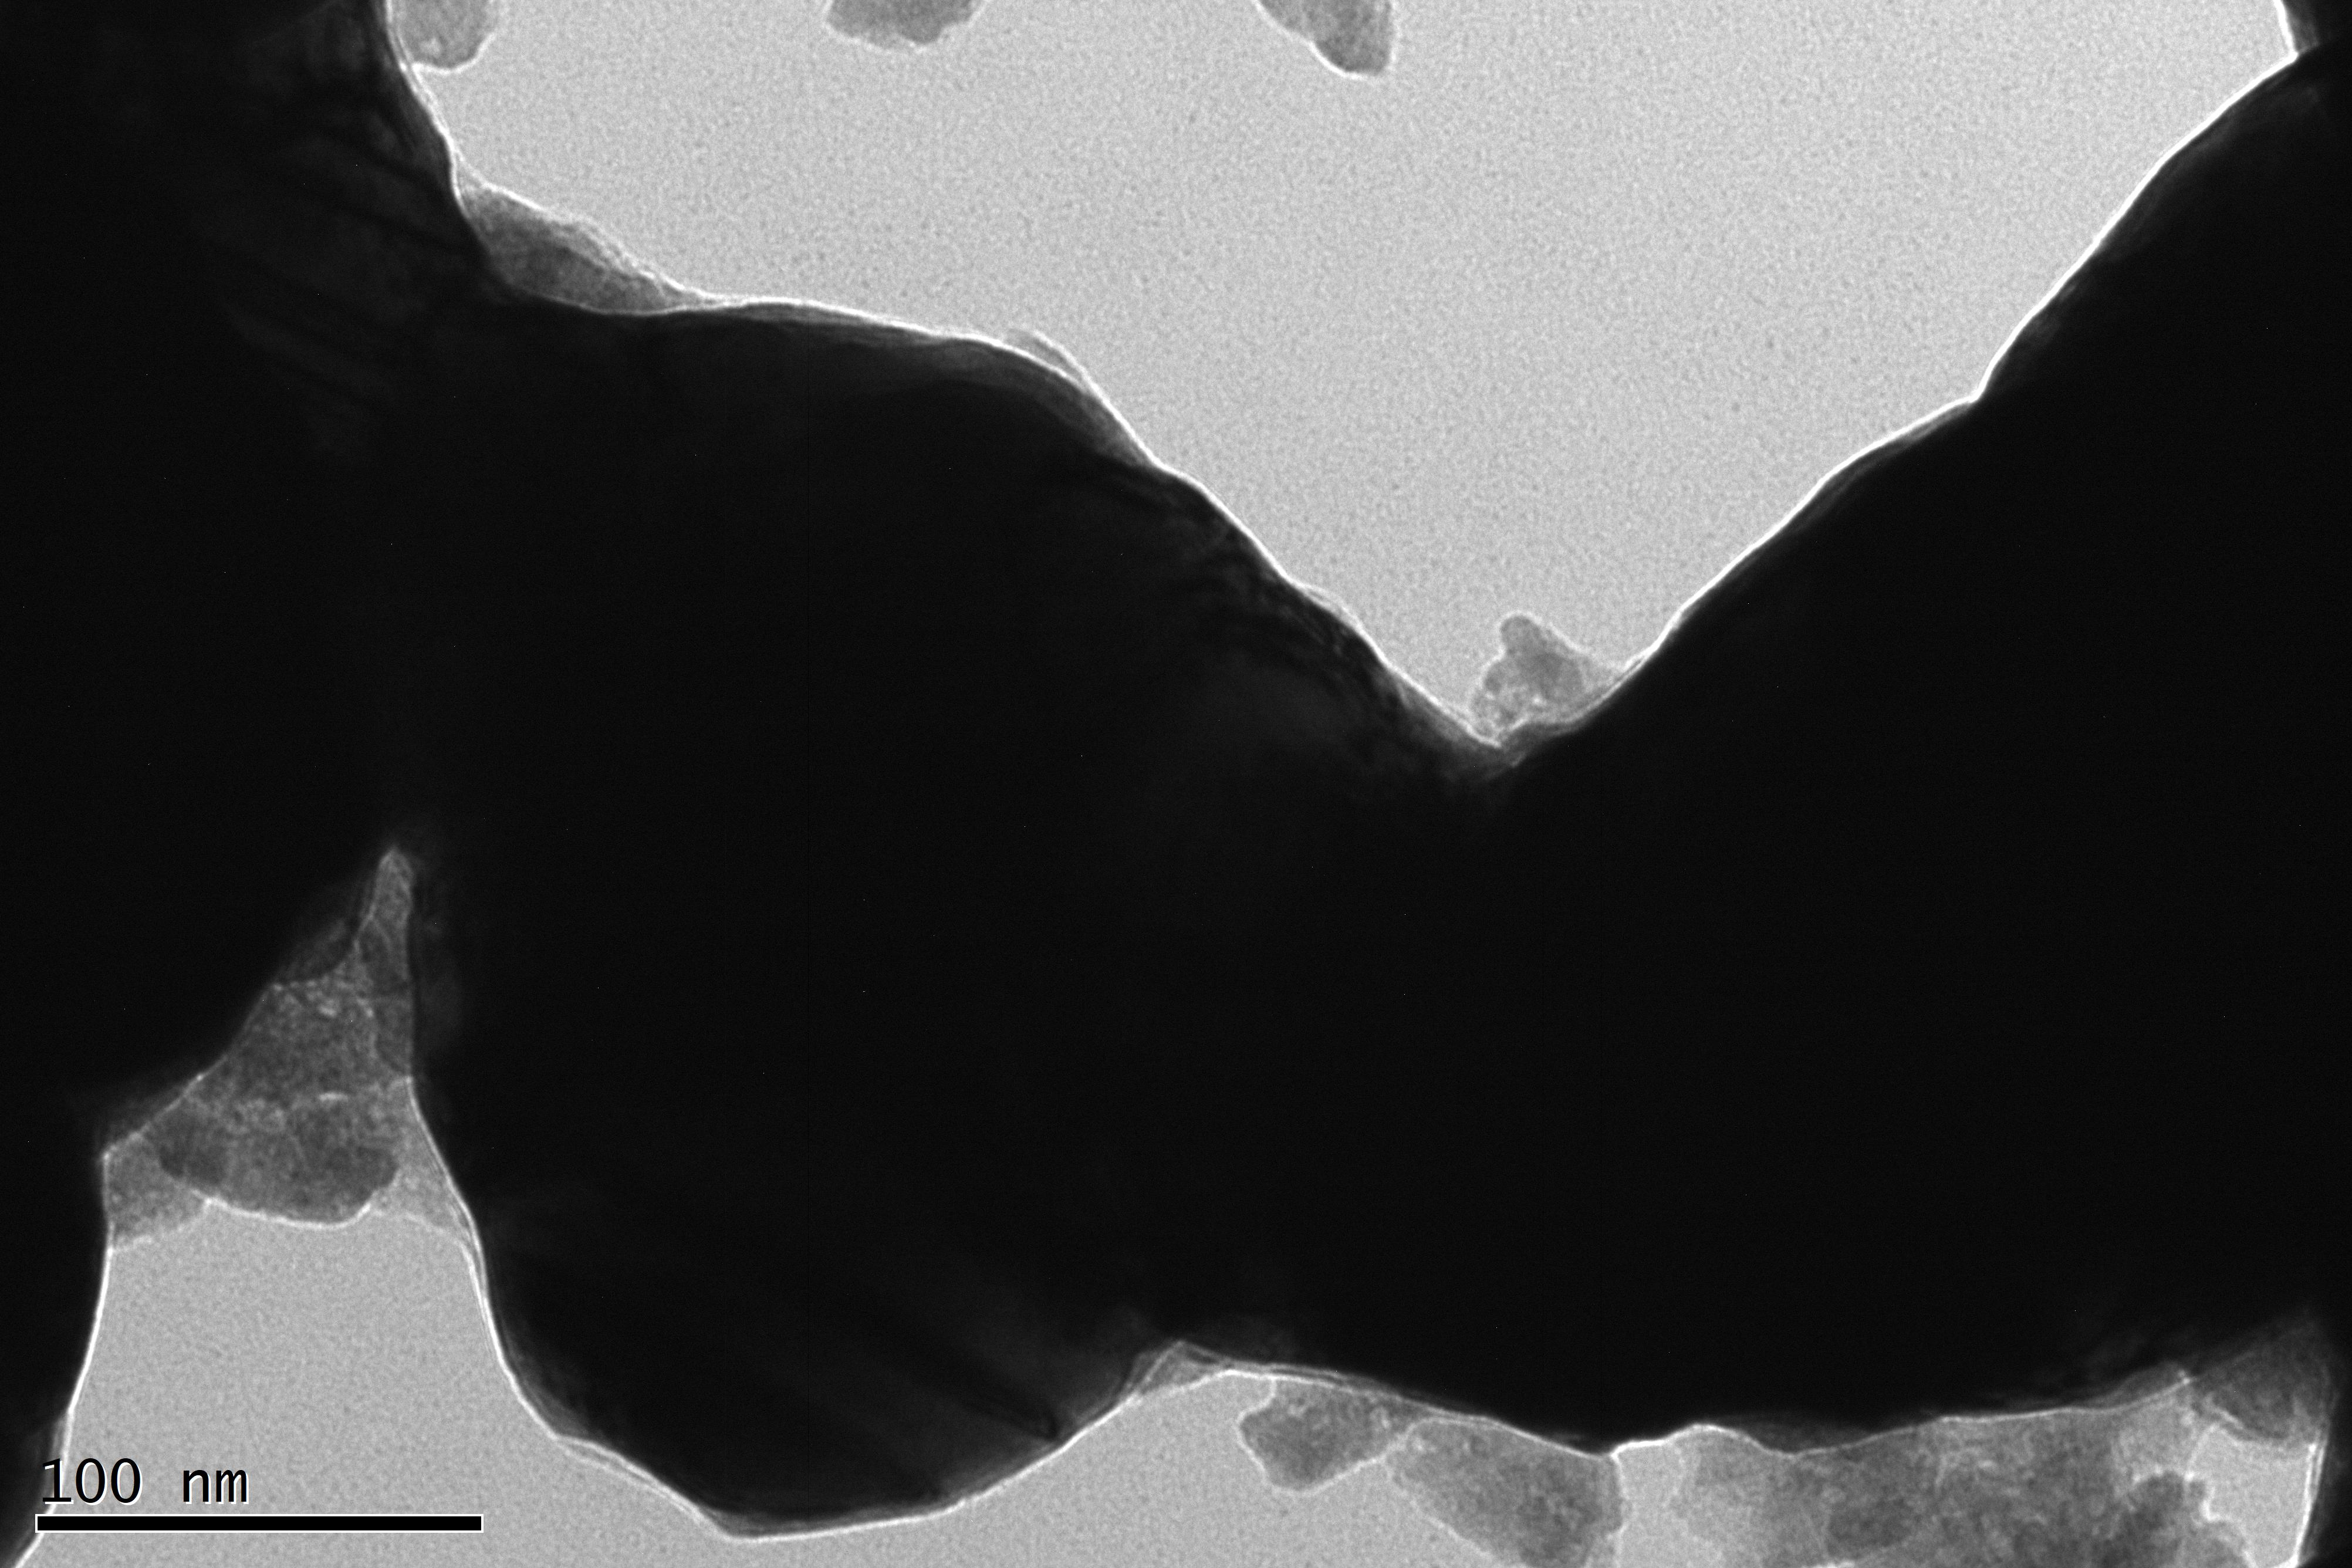
\includegraphics[width=0.45\linewidth]{Bilder/Gel-E-Cu_1}}
		\subfloat[\label{fig:Gel-E-Cu_2}]{%
			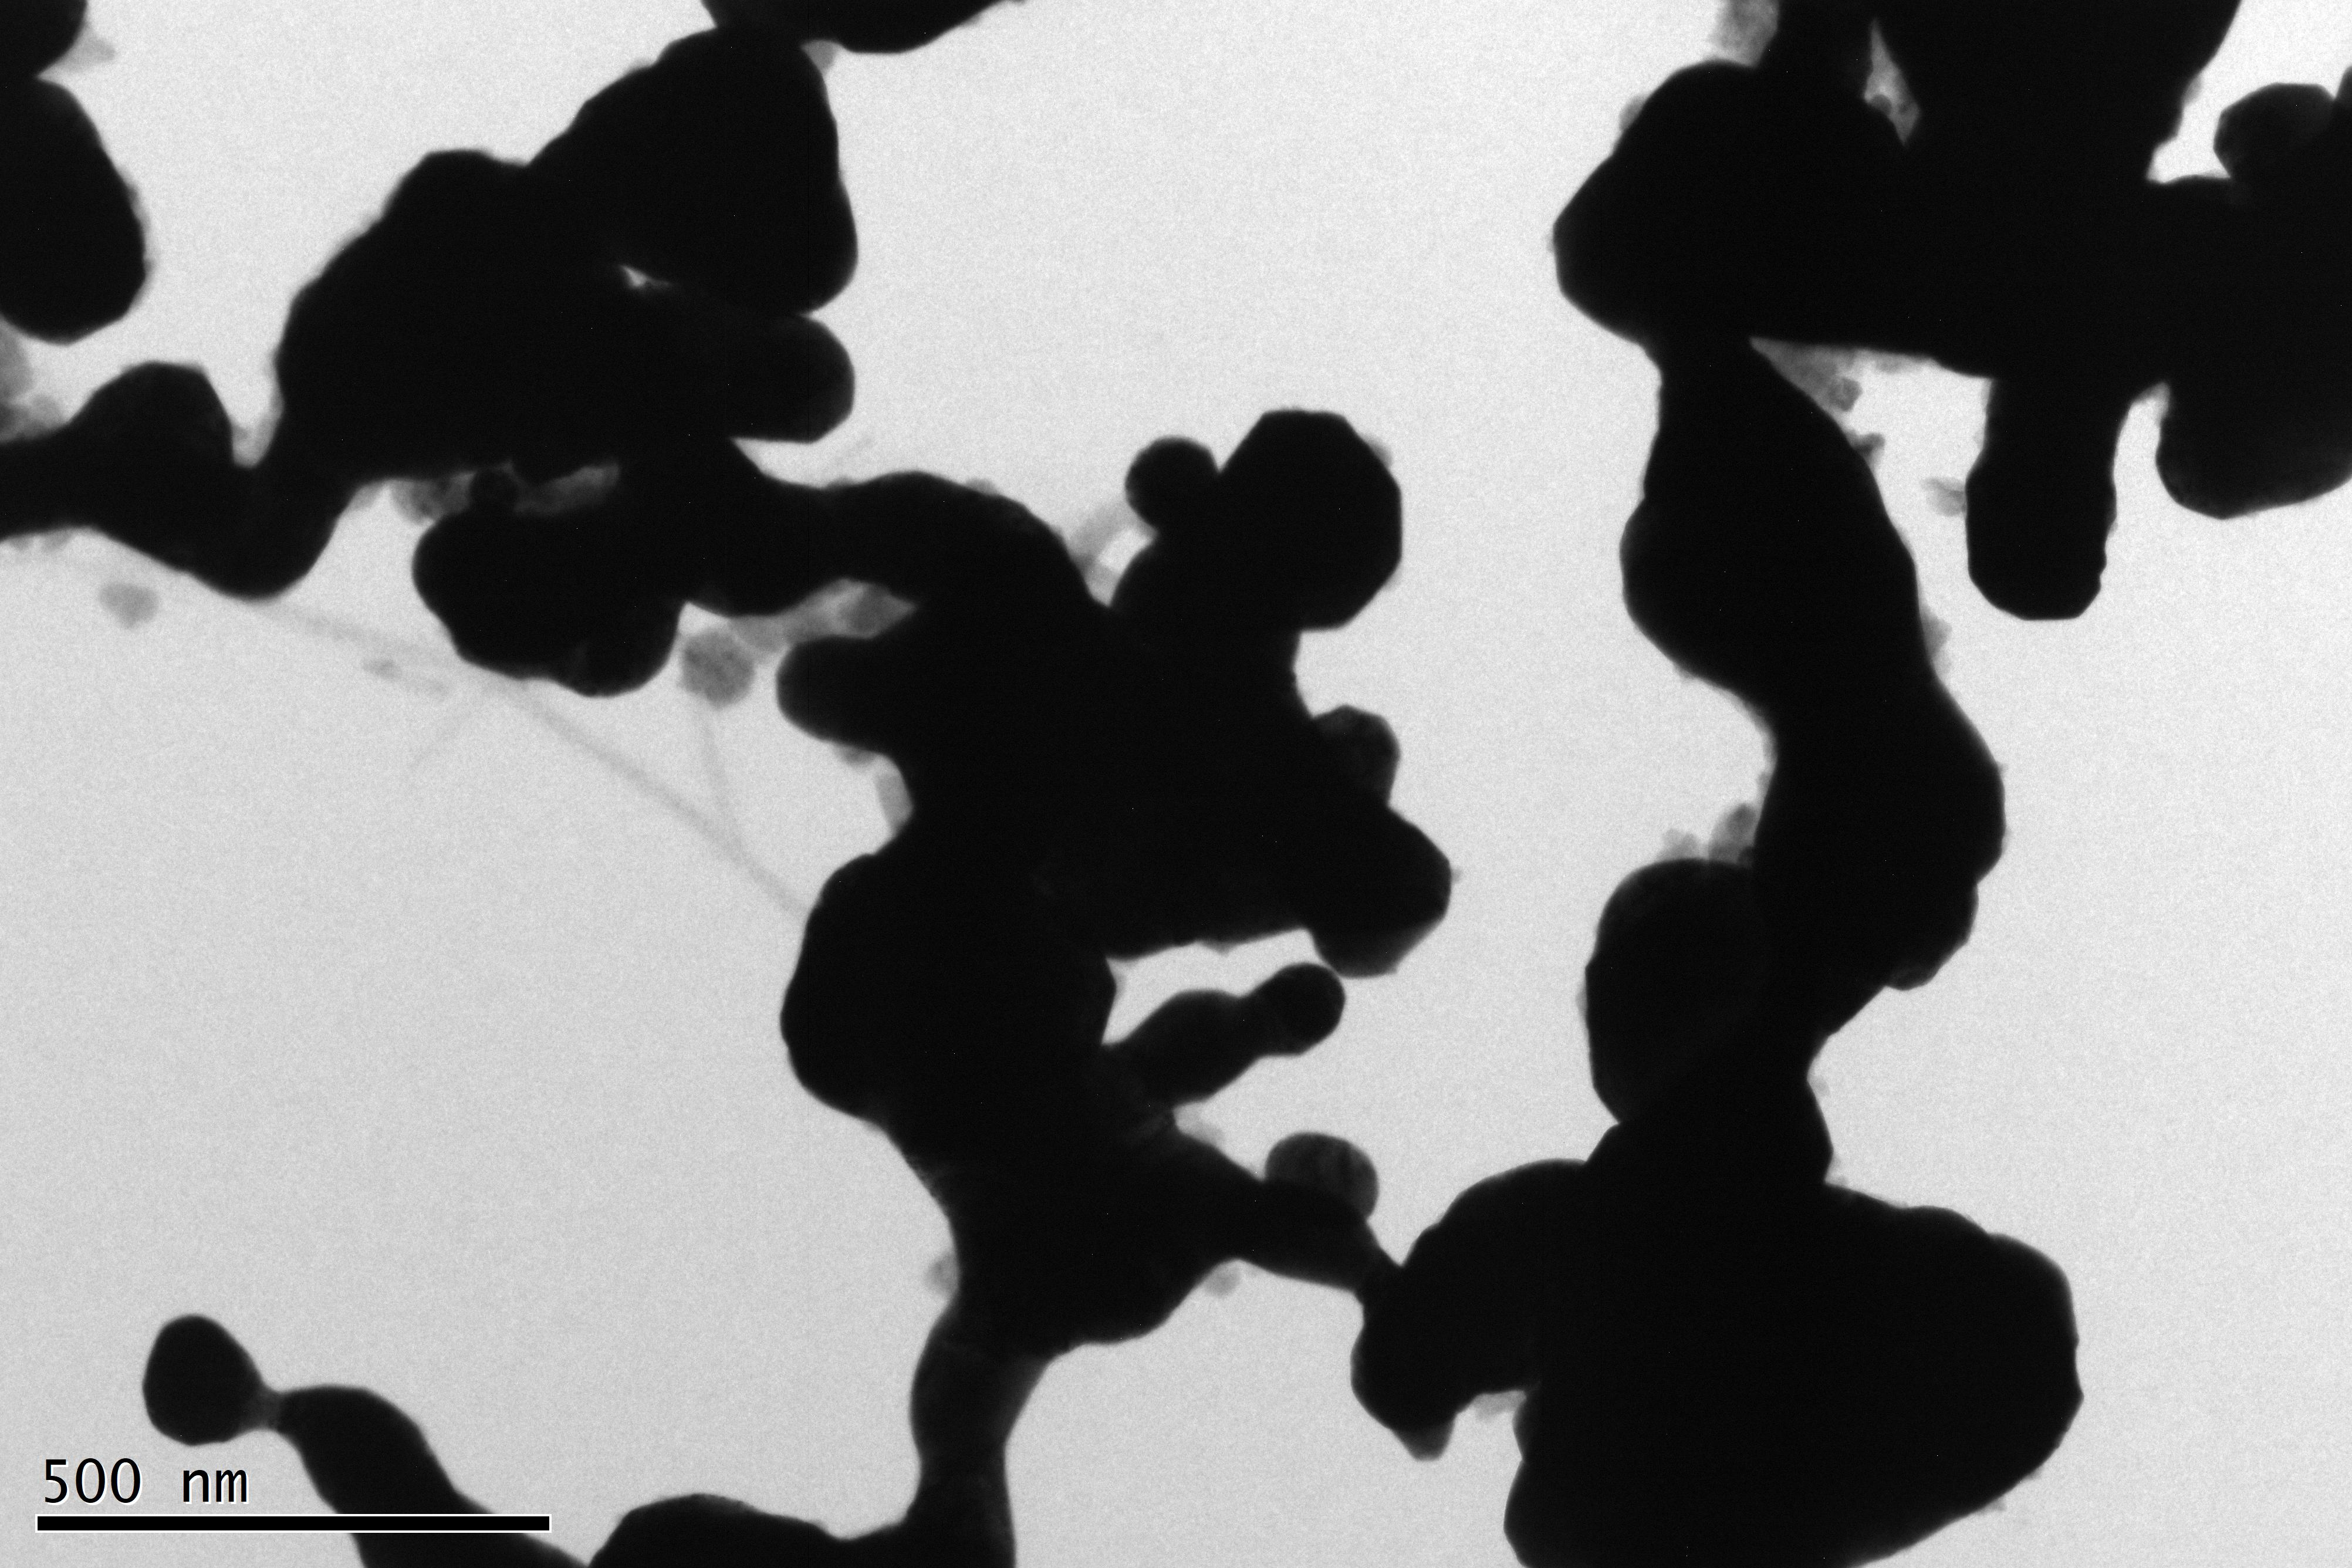
\includegraphics[width=0.45\linewidth]{Bilder/Gel-E-Cu_2}}
		\caption{TEM von einem ethanolischen Au-Gel mit CuS.}
		\label{fig:E-Cu}
	\end{figure}


	\subsubsection{Einfluss der Reaktionstemperatur}
		
		Bei den getesteten Gelen, die mit geringeren Temperaturen behandelt wurden, zeigt sich, dass bei geringeren Temperaturen, sich CuS wenig bis gar nicht an den Gelen bildet, wie in \cref{fig:Gel-E-Temp} gezeigt wird.
		Die Temperatur von \SI{250}{\degreeCelsius} scheint also nicht ausreichend um CuS aus der thermischen Zersetzung von \ch{Cu[DDTC]2} zu gewinnen, da auch neben den Gelen kein CuS gefunden werden konnte.
		Aus diesem Grund wurde auch bei späteren Versuchen nie von den \SI{290}{\degreeCelsius} abgewichen.
		\begin{figure}[H]
			\centering
			\subfloat[\label{fig:Gel-E-200C}]{%
				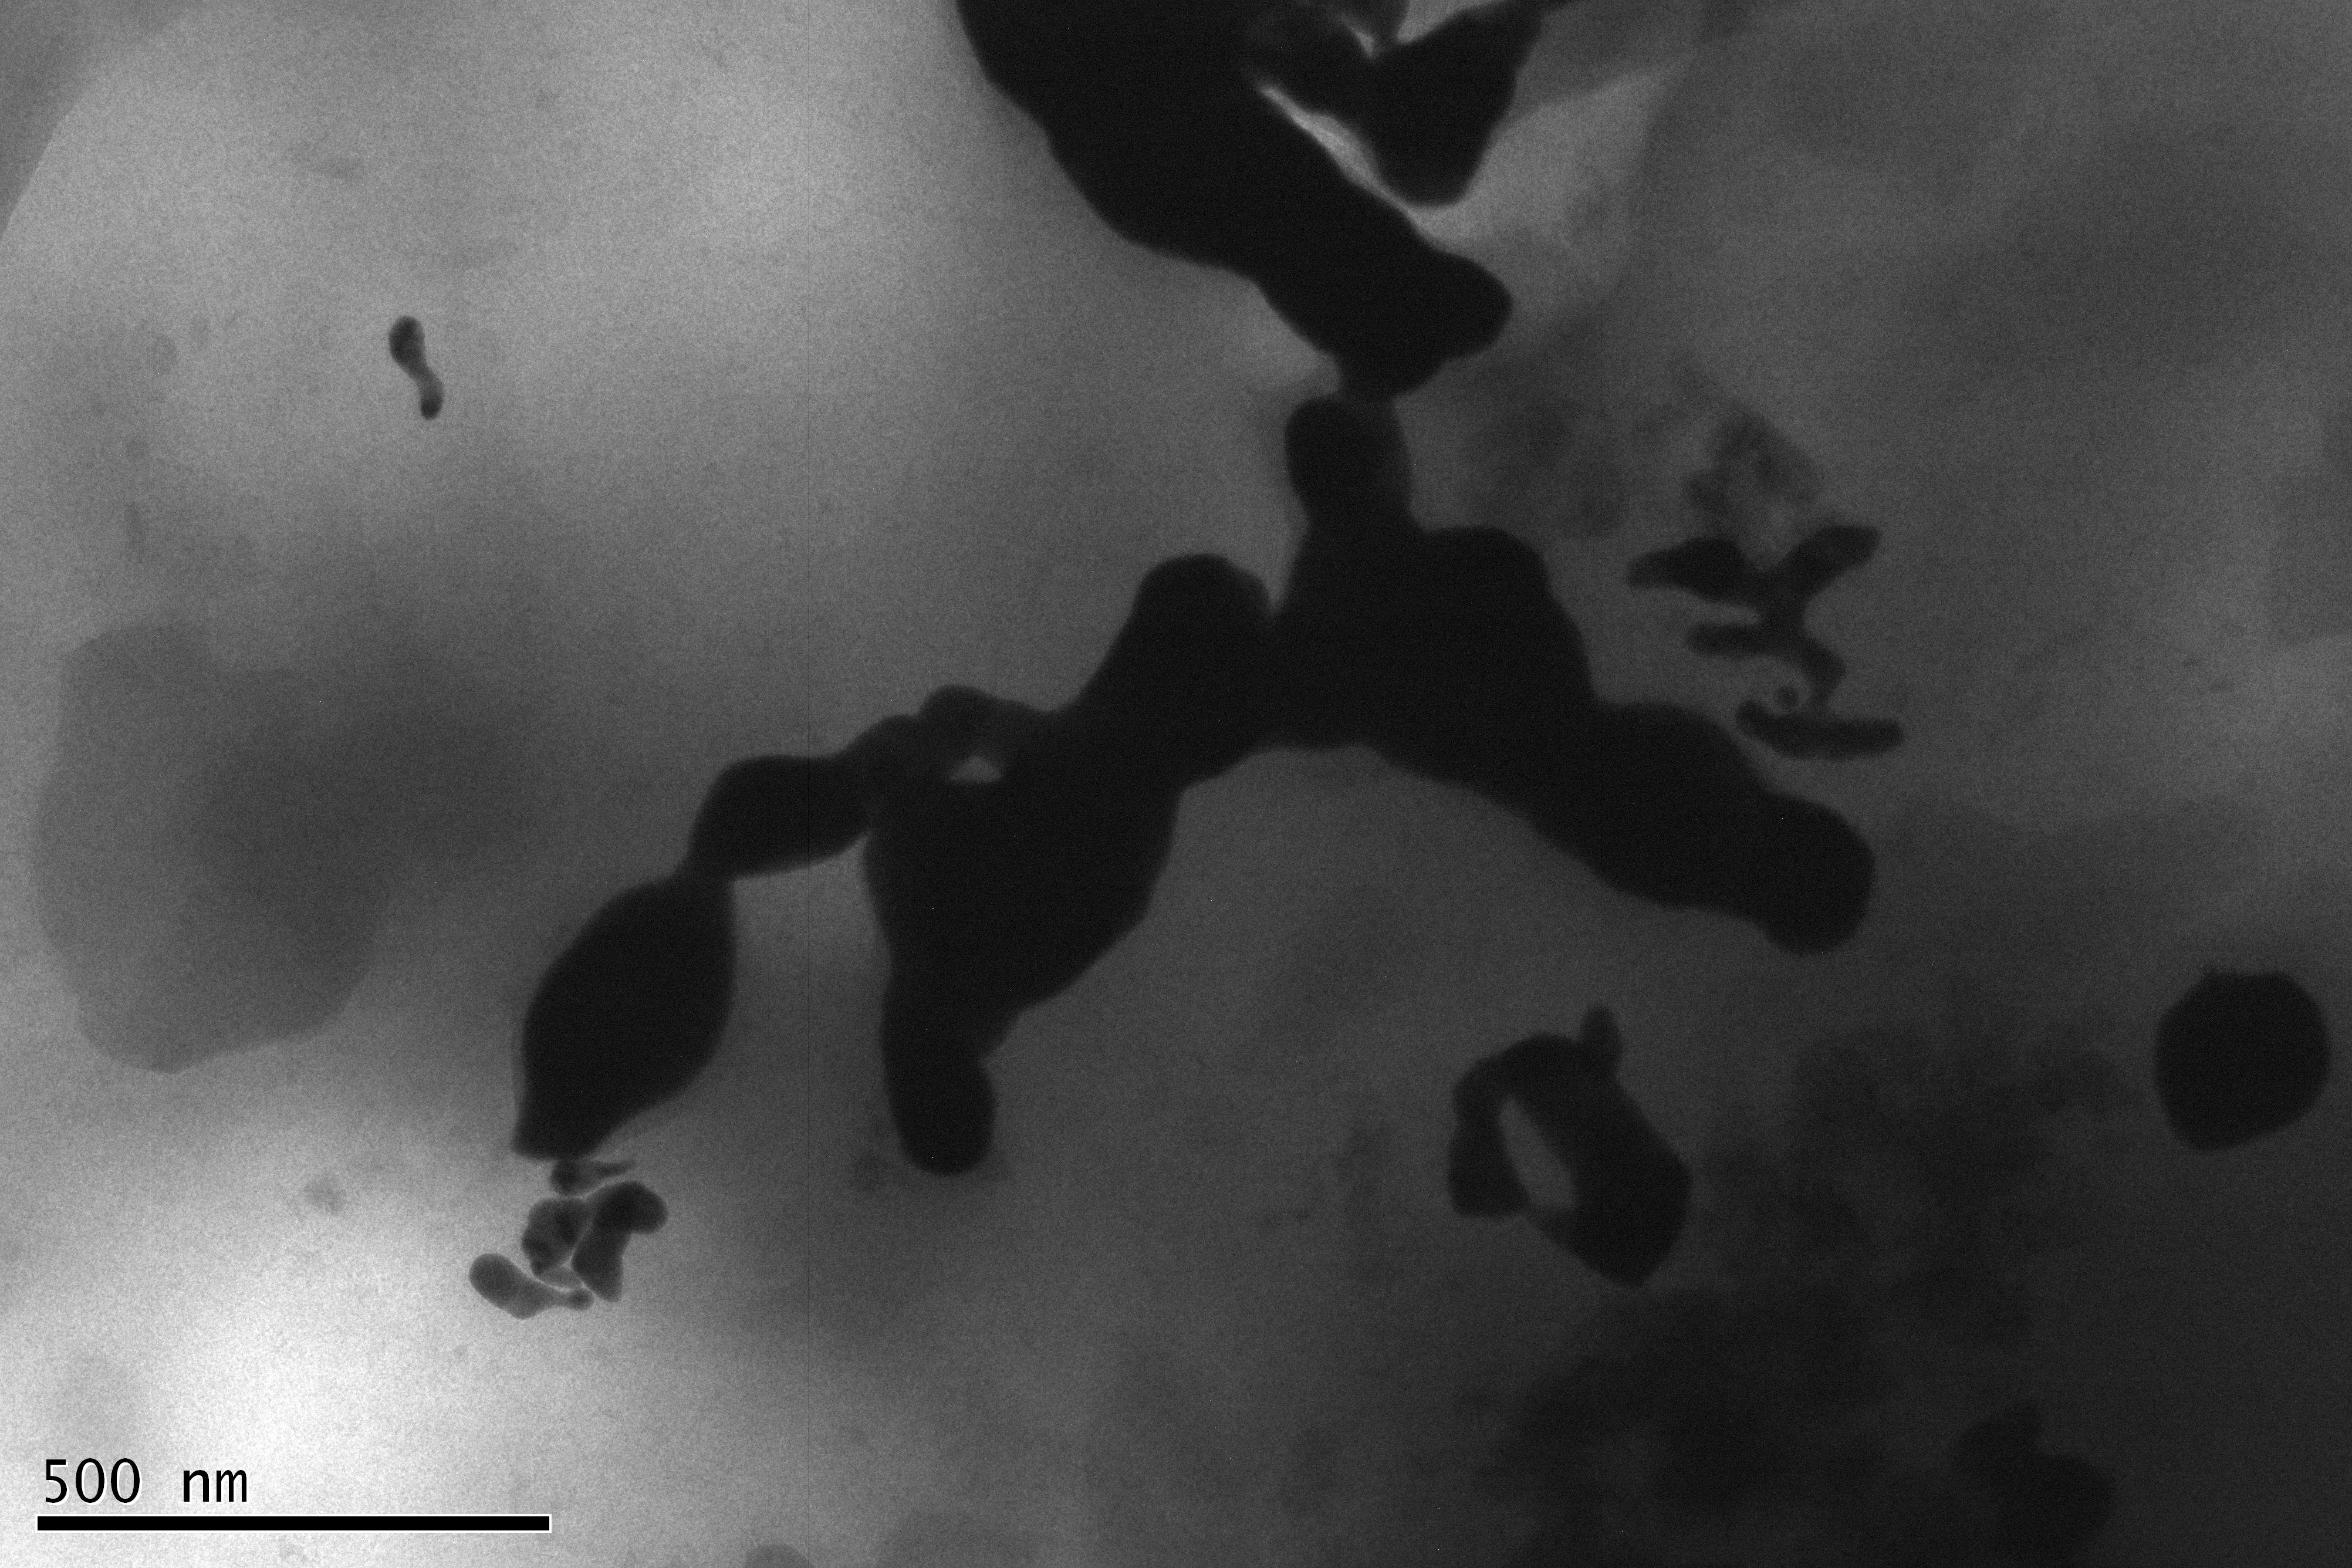
\includegraphics[width=0.45\linewidth]{Bilder/Gel-E-200C}}
			\subfloat[\label{fig:Gel-E-250C}]{%
				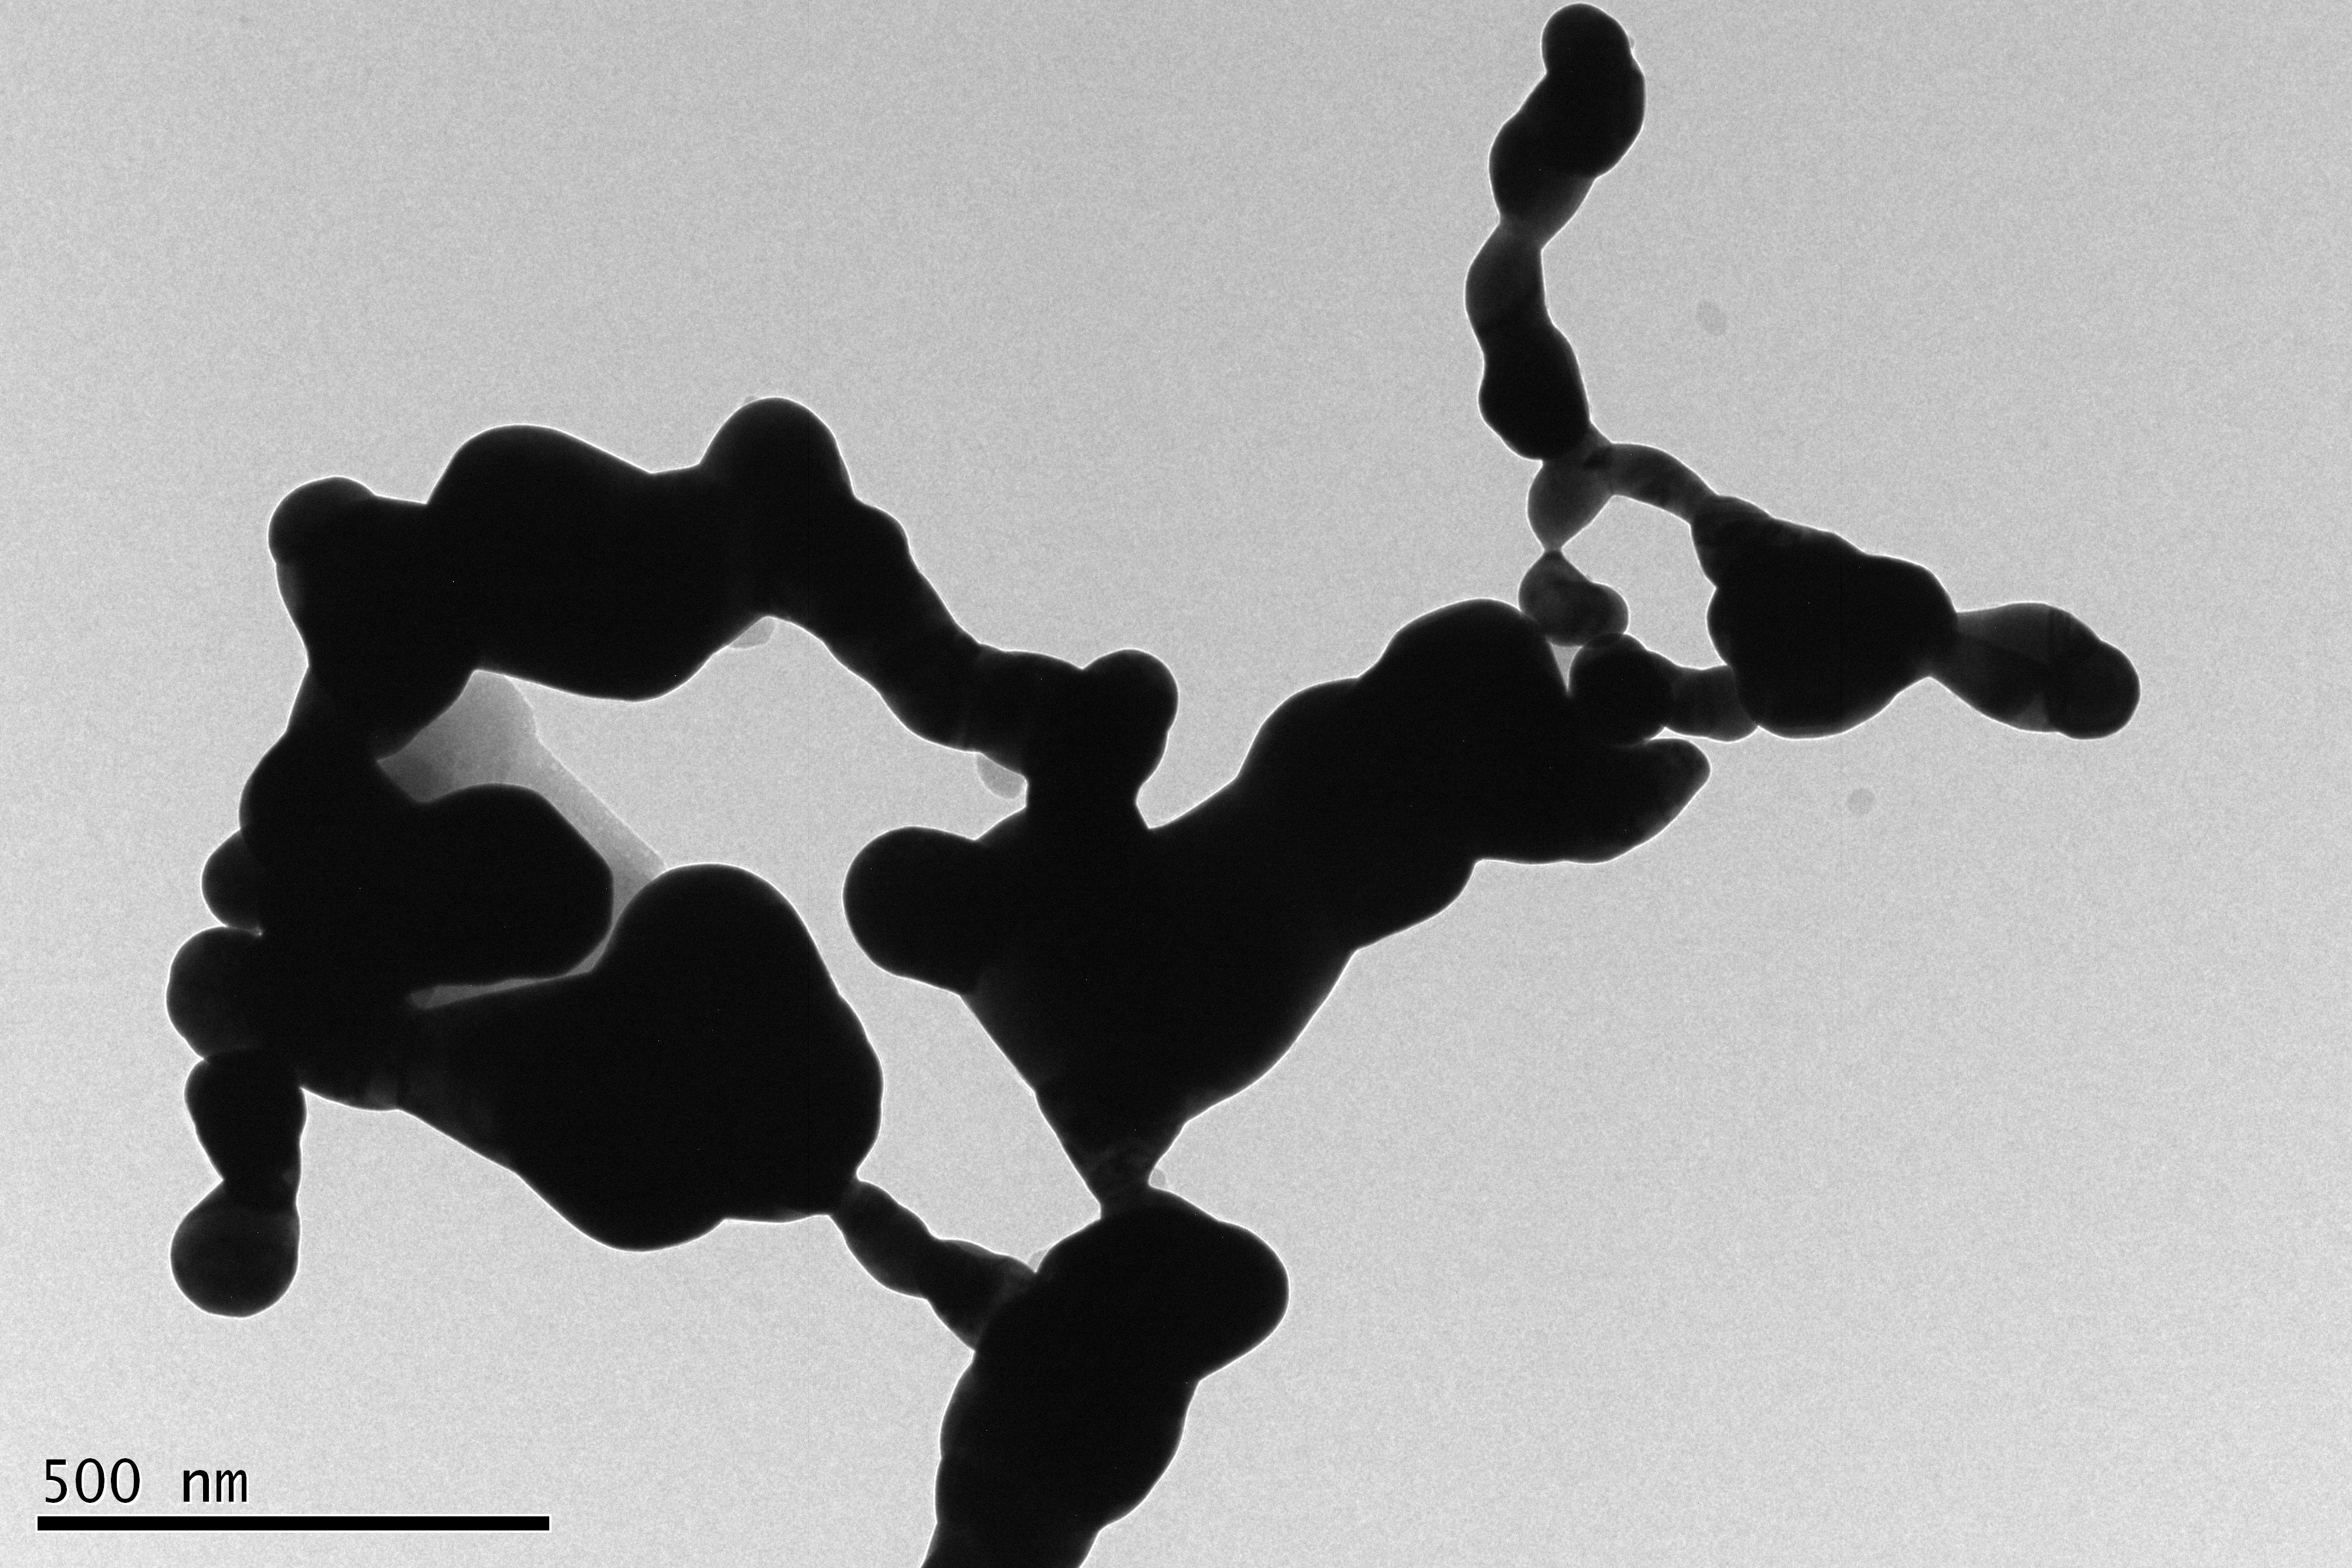
\includegraphics[width=0.45\linewidth]{Bilder/Gel-E-250C}}
			\caption{Gele nach der Reaktion mit \ch{Cu[DDTC]2} bei \emph{(a)}: \SI{200}{\degreeCelsius} und \emph{(b)}: \SI{250}{\degreeCelsius}.}
			\label{fig:Gel-E-Temp}
		\end{figure}
	
	\subsubsection{Variation des Kations}
	
		Da es ein Ziel war ein möglichst variablen Mechanismus für das anwachsen zu entwickeln, wurde neben \ch{Cu[DDTC]2} auch die gleiche Reaktion mit \ch{Cd[DDTC]2} und \ch{Zn[DDTC]2} untersucht.
		
		Im Gegensatz zum \ch{Cu[DDTC]2} zeigt sich bei gleichem Versuchsaufbau und Durchführung bei \ch{Cd[DDTC]2} ein deutlich anderes Bild.
		es wurden hier nicht nur einzelne  kleine Zwischenräume mit CdS bedeckt, sondern es kommt zu einer fast kompletten Ummantelung des Gels wie in \cref{fig:Gel-E-CdS} zu erkennen ist.
		Allerdings hat sich auch ein Teil des CdS neben dem Gel gebildet. 
		Dies ist sowohl in den TEM-Aufnahmen zu erkennen aber auch schon mit bloßem Auge lässt sich die typische Gelbfärbung vom CdS am kompletten Boden des Reaktionsgefäßes auch neben dem Gel erkennen, wie in \cref{fig:Foto-CdS}.
		\begin{figure}[htbp]
			\centering
			\subfloat[\label{fig:Gel-E-CdS_1}]{%
				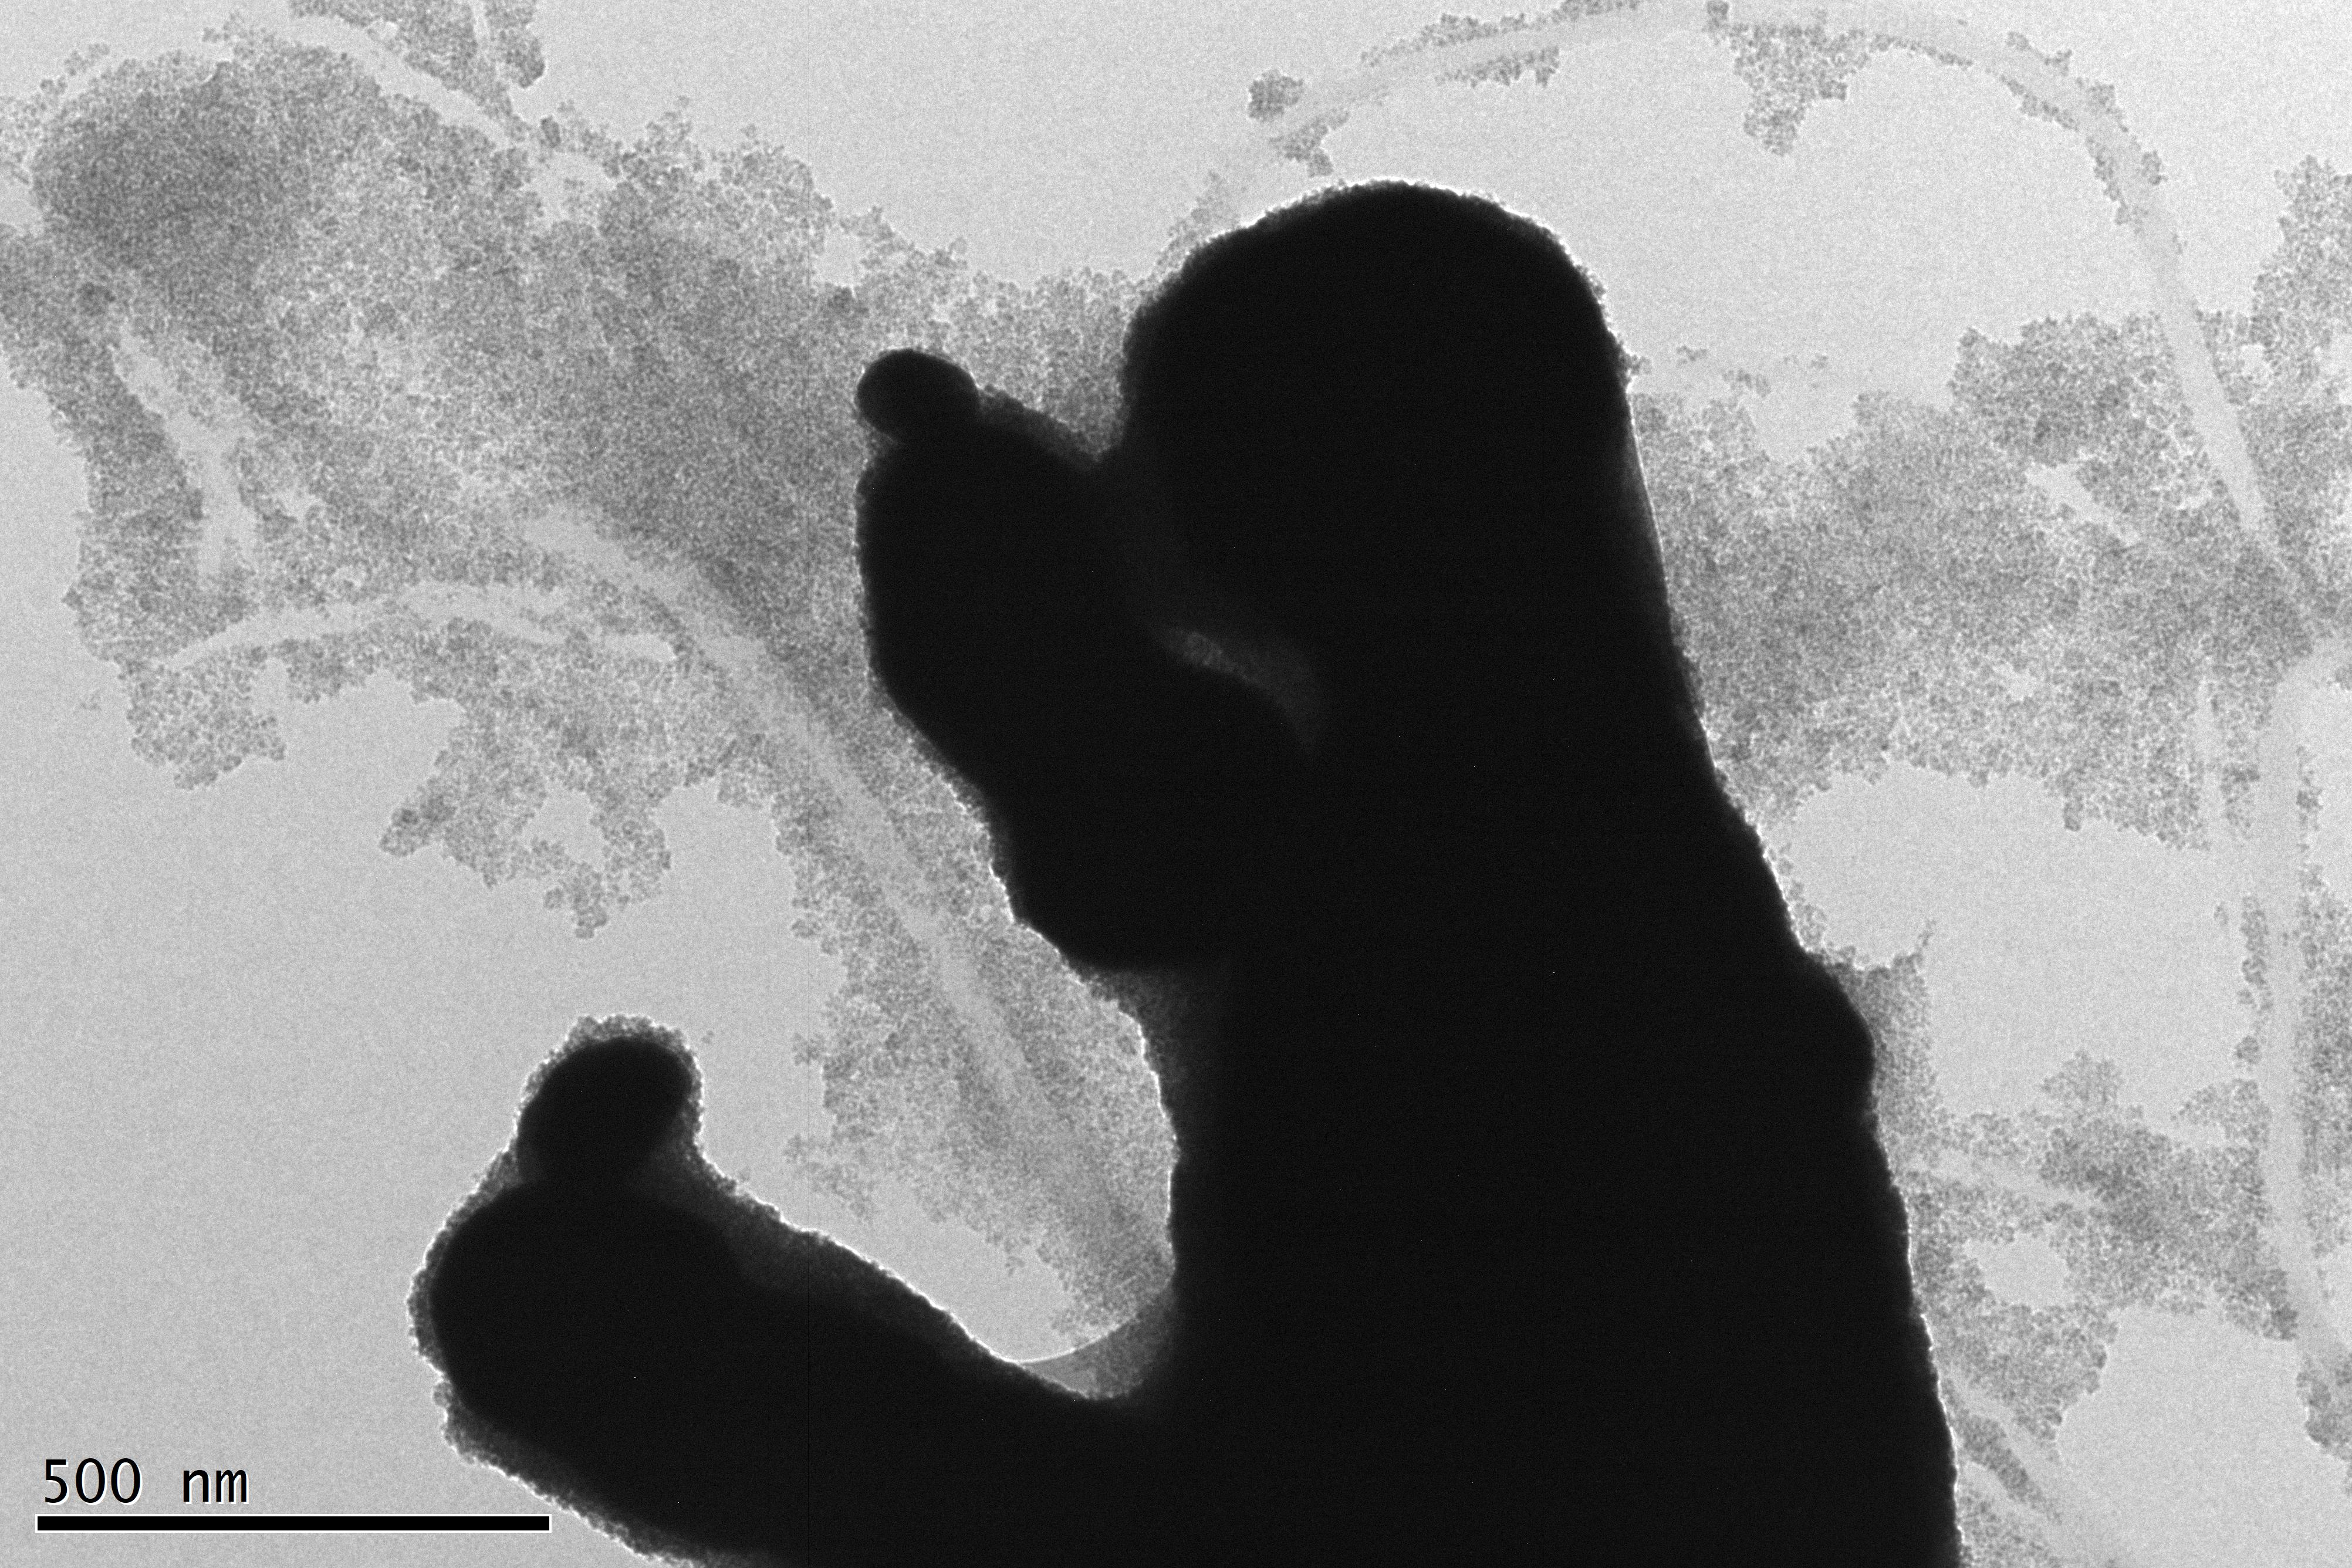
\includegraphics[width=0.33\linewidth]{Bilder/Gel-E-CdS_1}}
			\subfloat[\label{fig:Gel-E-CdS_2}]{%
				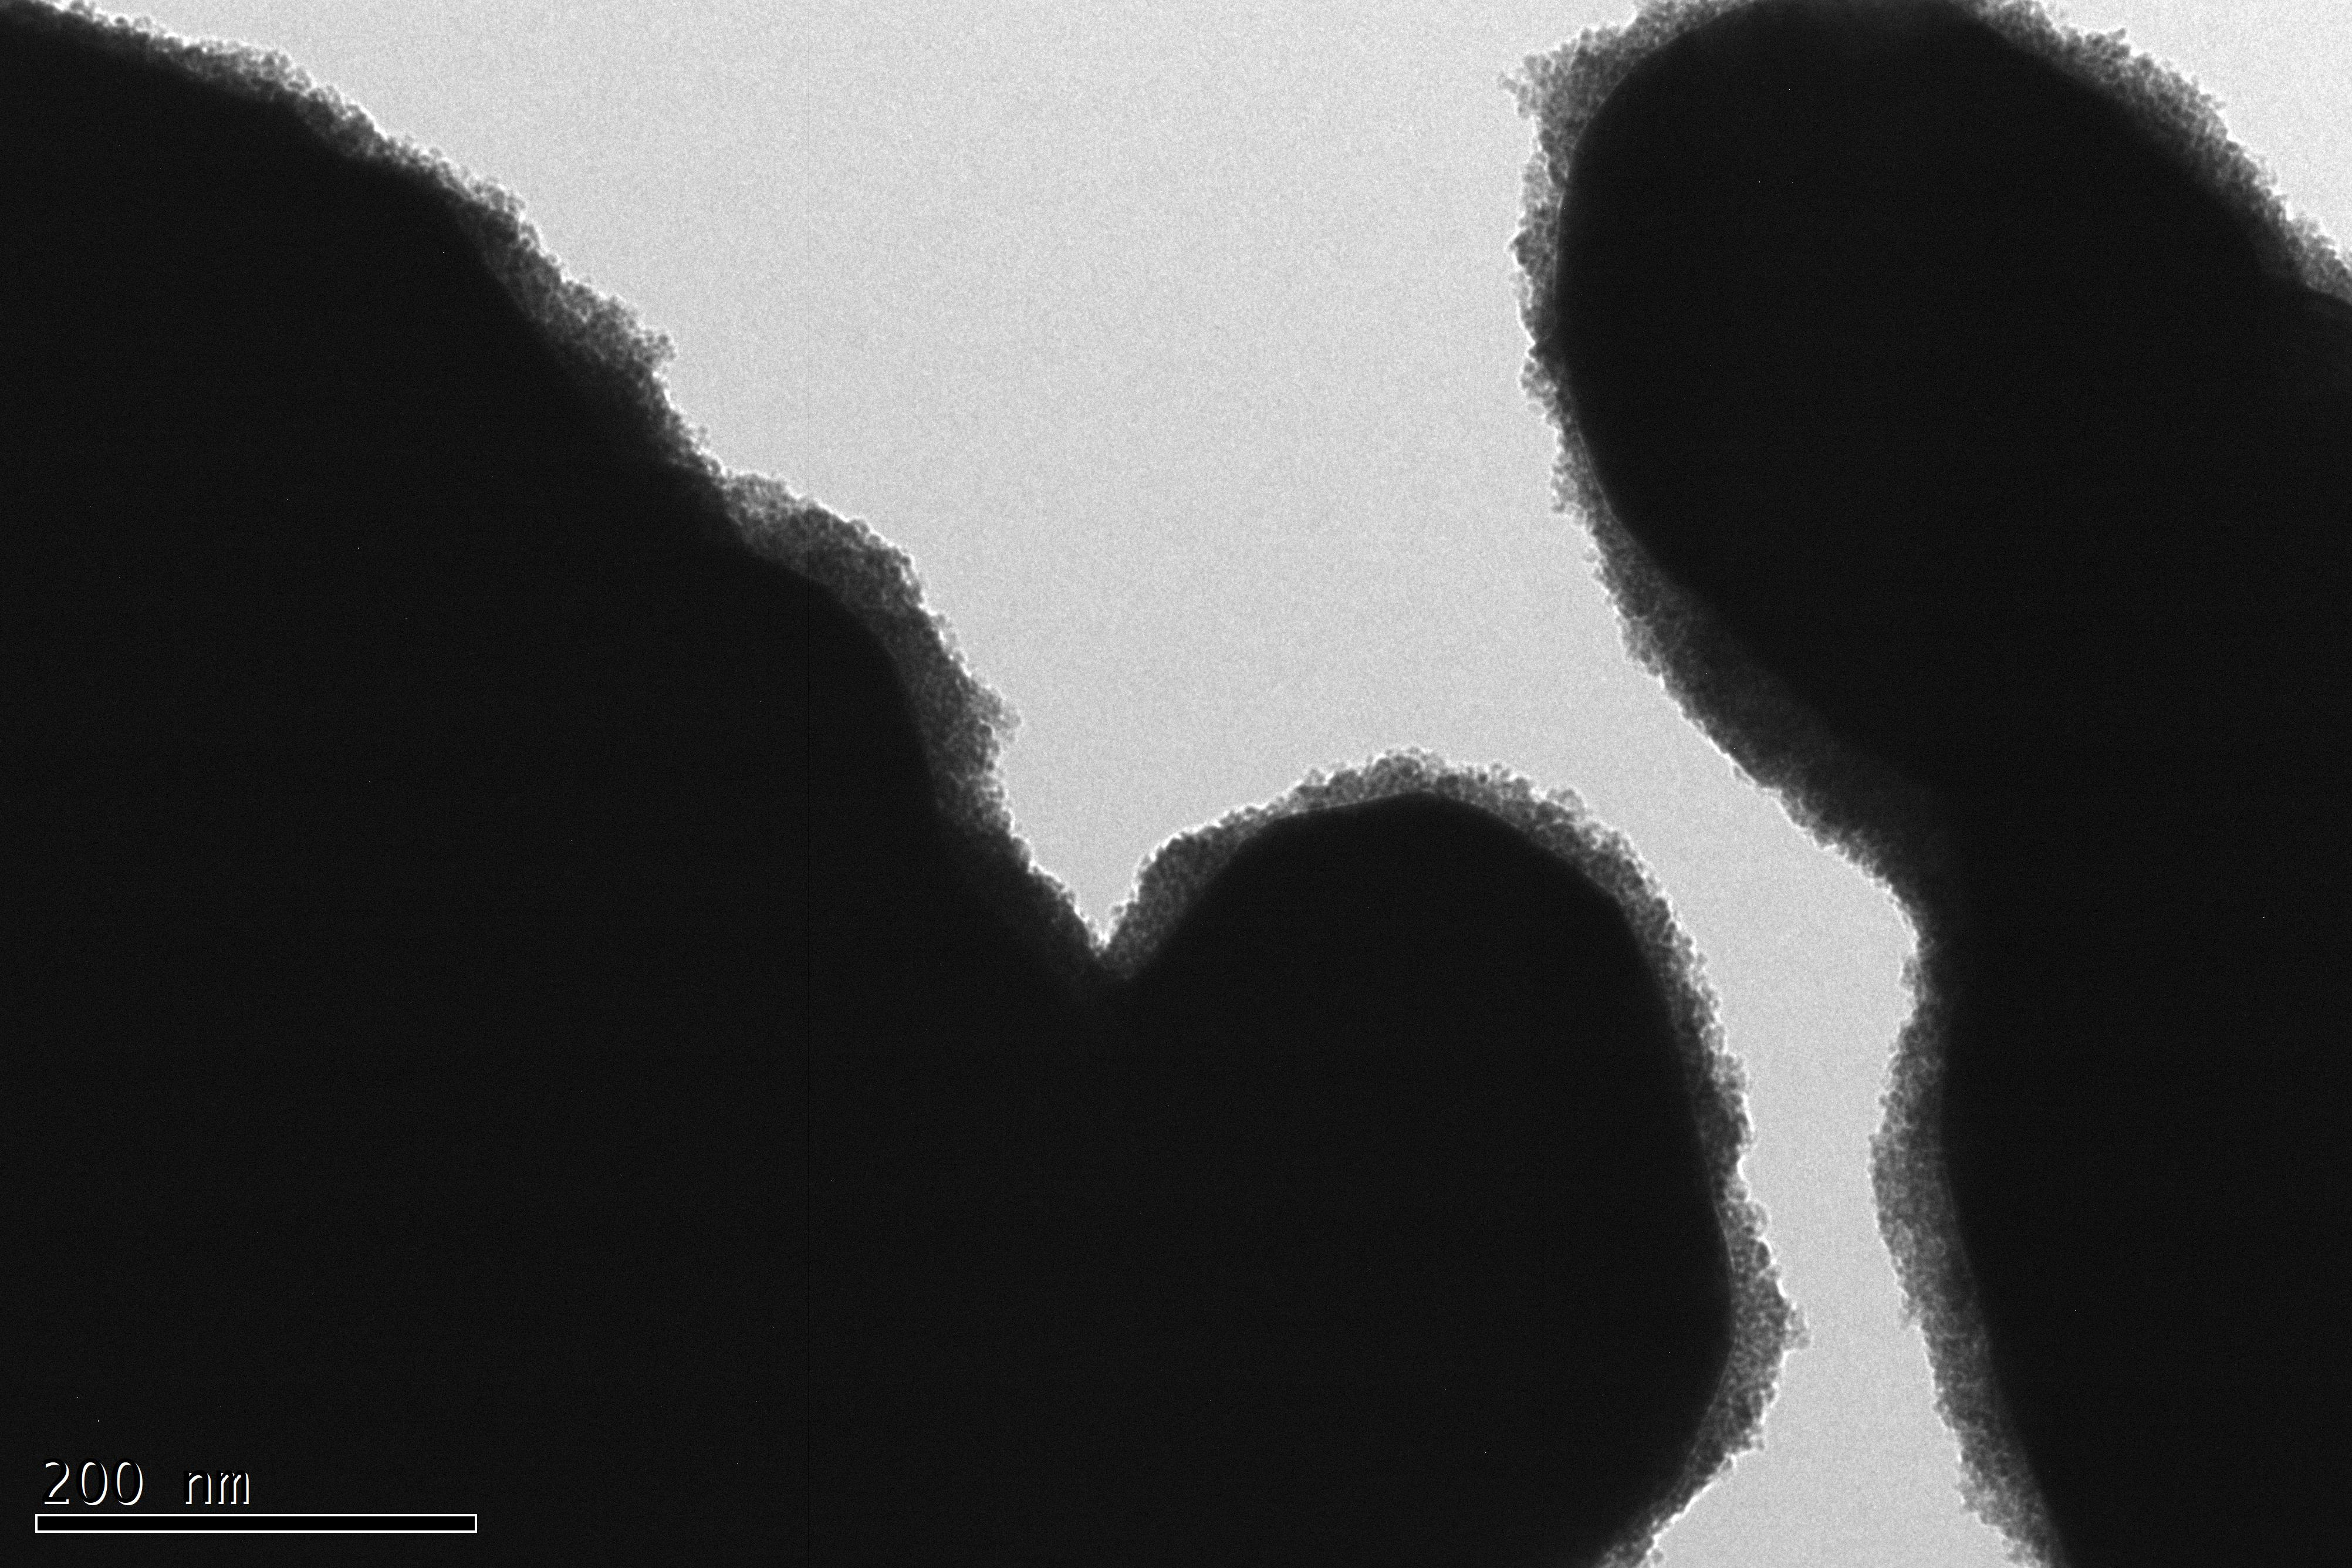
\includegraphics[width=0.33\linewidth]{Bilder/Gel-E-CdS_2}}
			\subfloat[\label{fig:Gel-E-CdS_3}]{%
				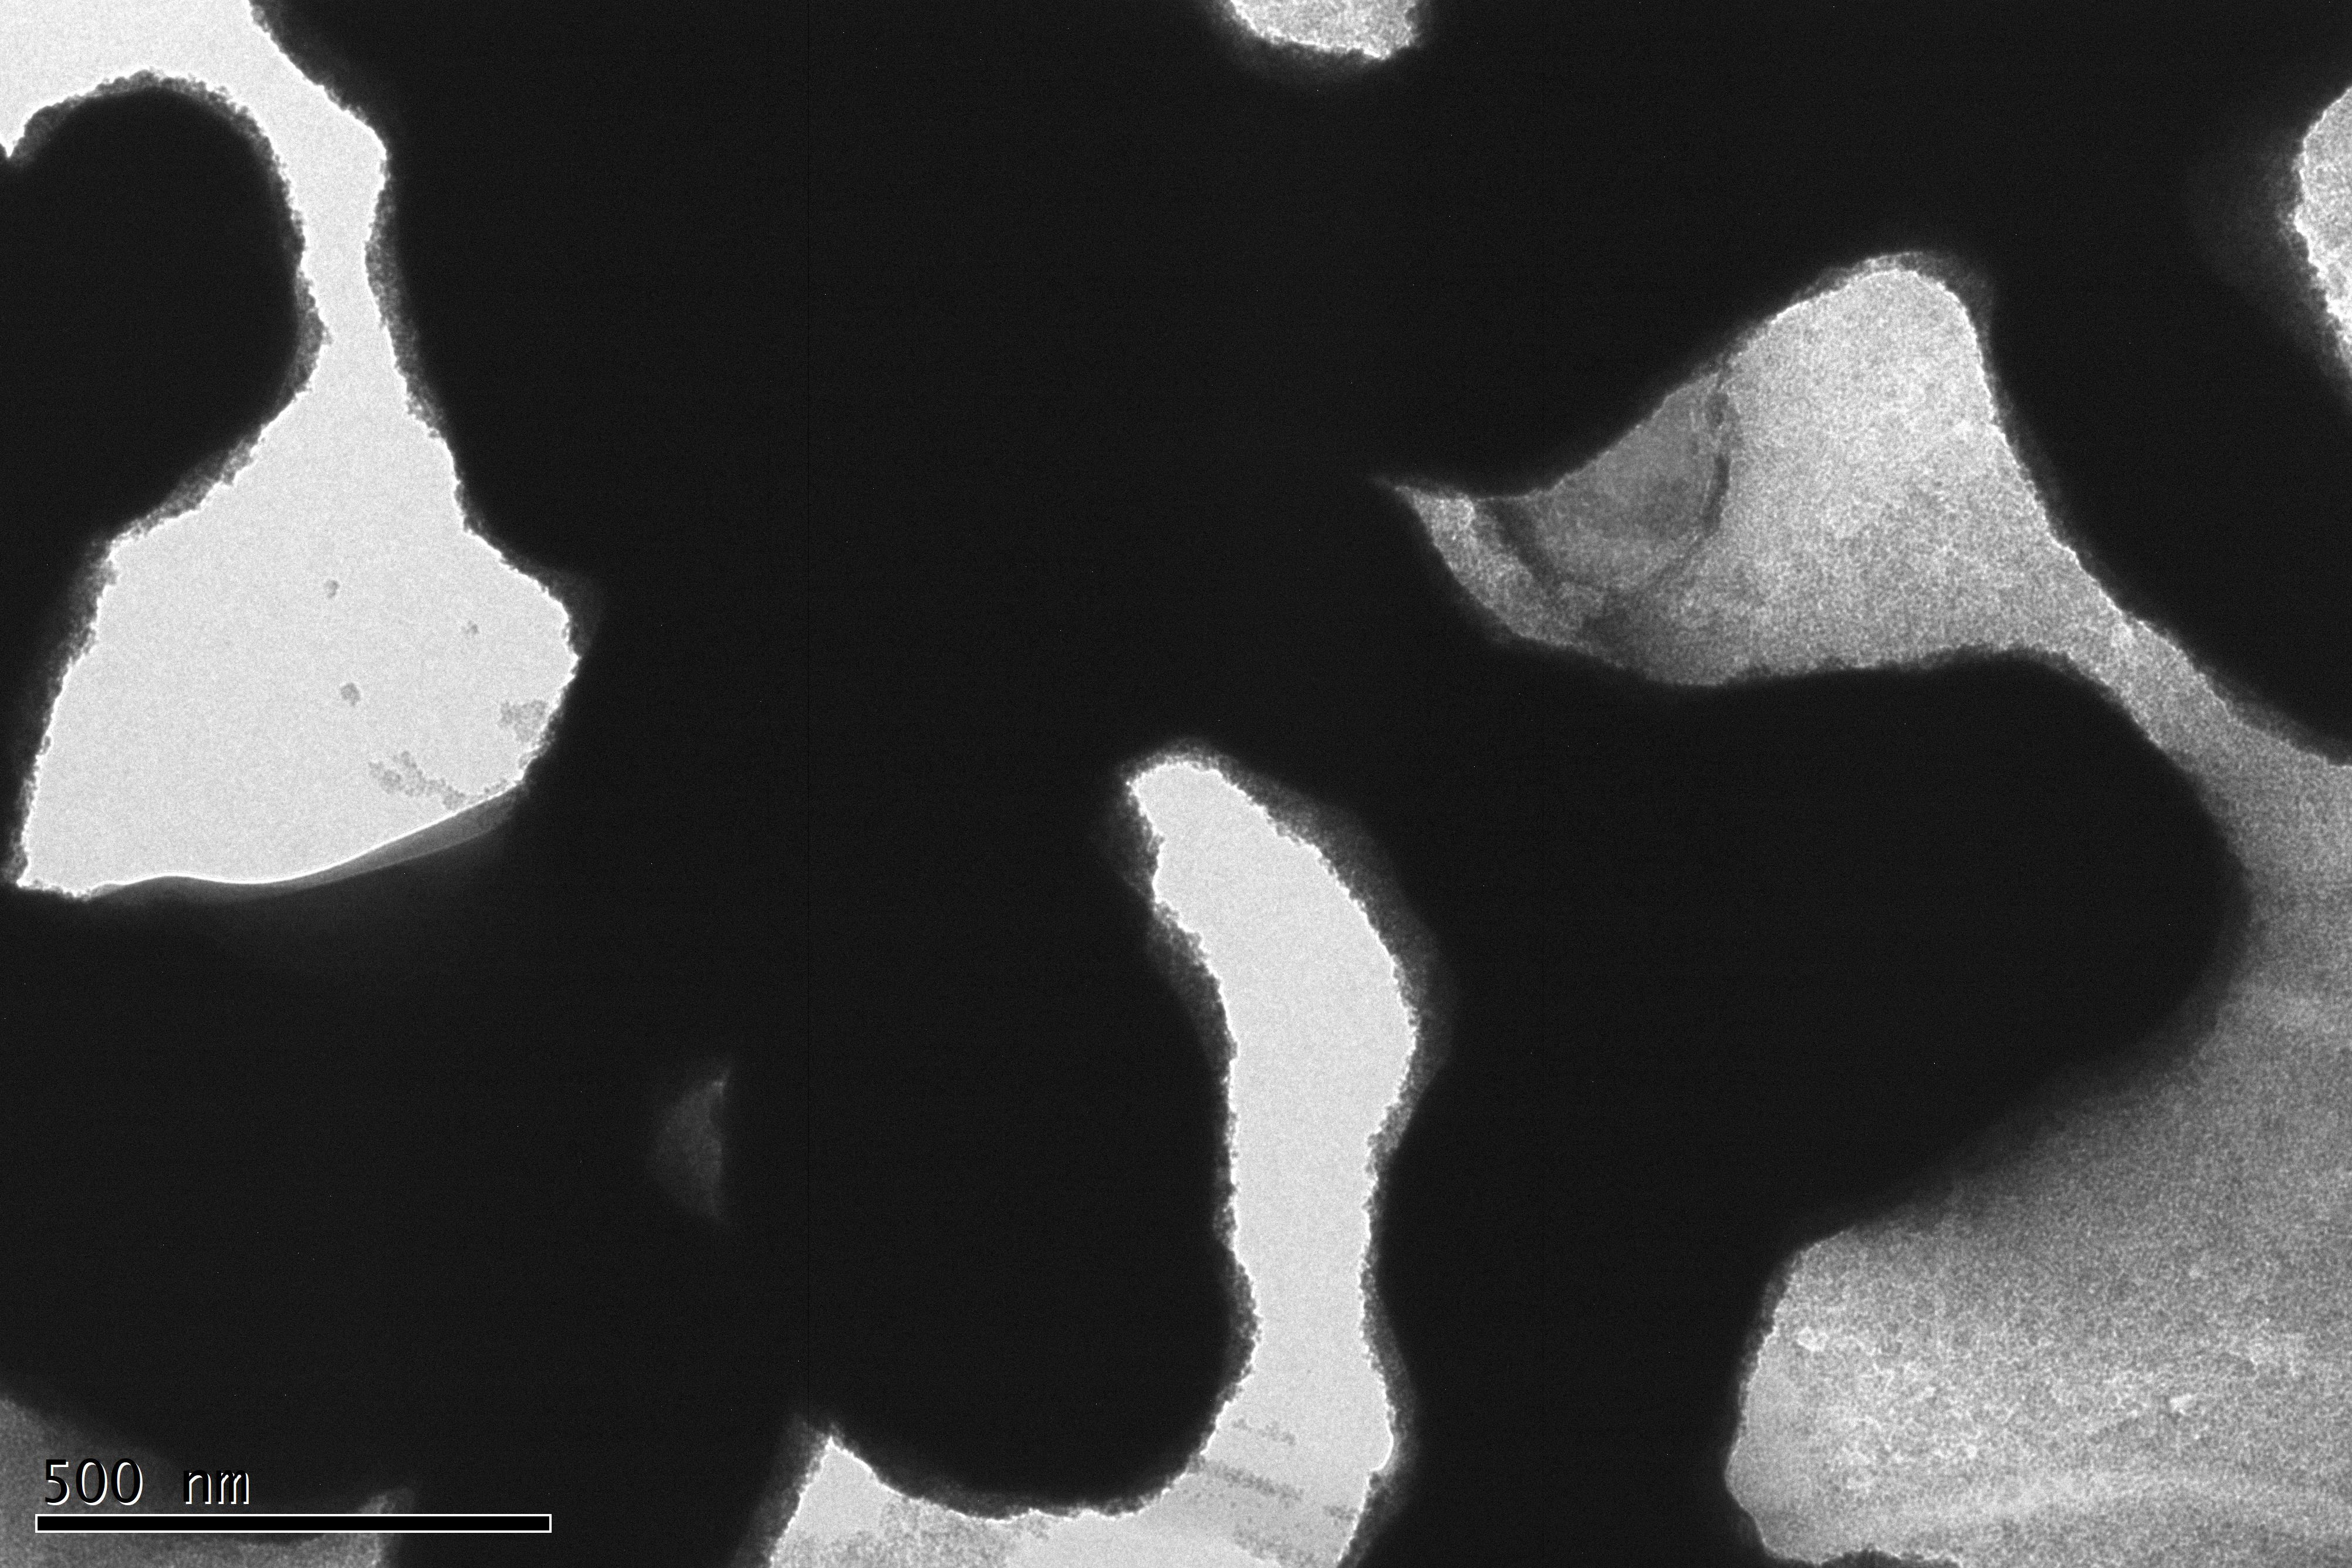
\includegraphics[width=0.33\linewidth]{Bilder/Gel-E-CdS_3}}
			\caption{TEM-Aufnahmen der Gele nach der thermischen Zersetzung von \ch{Cd[DDTC]2} zu CdS.}
			\label{fig:Gel-E-CdS}
		\end{figure}
	
		\begin{figure}[H]
			\centering
			\includegraphics[width=0.6\textwidth]{Bilder/Foto-CdS} 	
			\caption{Das Gel nach der Reaktion von \ch{Cd[DDTC]2}. Die typische Gelbfärbung von CdS ist deutlich zu erkennen.}
			\label{fig:Foto-CdS}
		\end{figure}
		
		Das Absorptionsspektrum, des mit \ch{Cd[DDTC]2} behandelten Gels, das in \cref{fig:UV-Gel-E-CdS} dargestellt ist, zeigt ein Maximum bei \SI{440}{\nano\meter}. 
		Dieses Absorptionsmaximum ist energetisch deutlich  höher als die Bandlücke des CdS als Bulk. 
		Da die CdS-Partikel jedoch, wie auf den TEM-Aufnahmen zu erkennen ist, sehr klein sind ($<$\SI{5}{\nano\meter}), kann dies durch den Größenquantisierungseffekt erklärt werden.
		
		\begin{figure}[H]
			\centering
			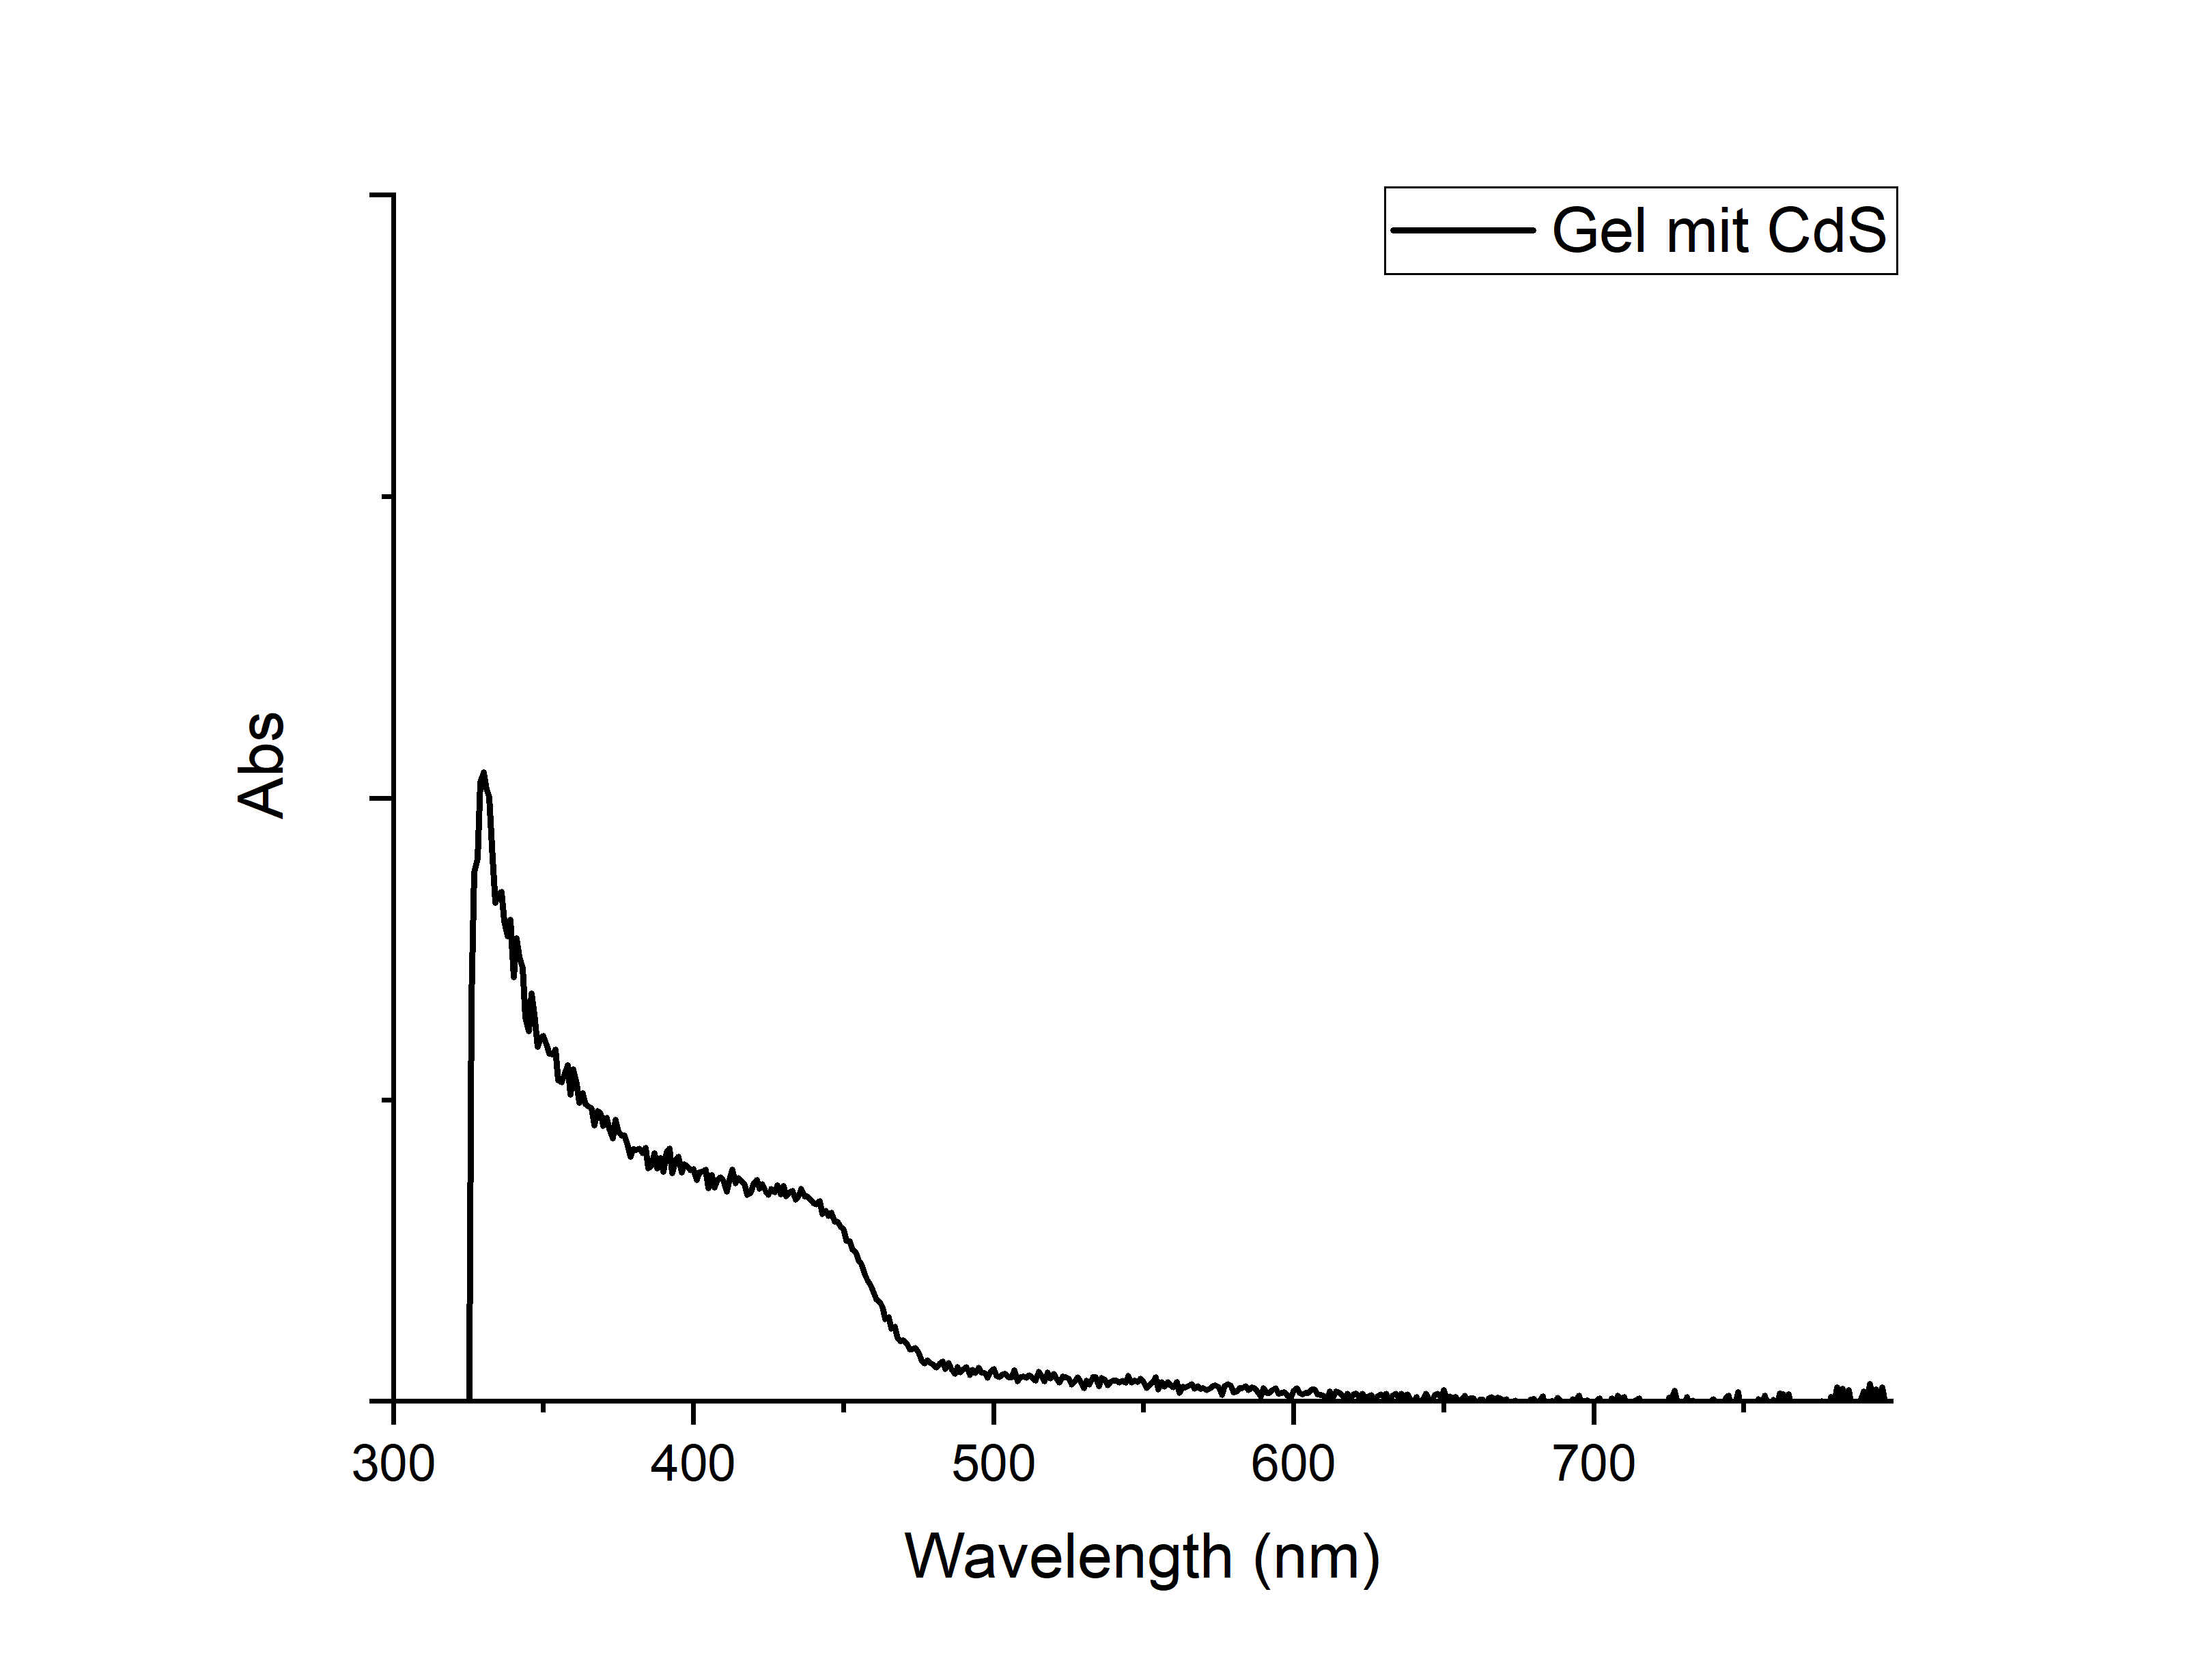
\includegraphics[width=0.6\textwidth]{Bilder/UV-Gel-E-CdS} 	
			\caption{Absorptionsspektrum des Gels, das mit \ch{Cd[DDTC]2} behandelt wurde.}
			\label{fig:UV-Gel-E-CdS}
		\end{figure}
	
		Während bei der Probe mit \ch{Cd[DDTC]2} eine fast komplette Schale um das Gel beobachtet werden konnte, waren die Ergebnisse bei der Behandlung mit \ch{Zn[DDTC]2} deutlich anders.
		So lassen sich bei den TEM-Aufnahmen, die in \cref{fig:Gel-E-ZnS} keine Partikel am Gel erkennen und auch das Absorptionsspektrum zeigte nichts, wie \cref{fig:UV-Gel-E-ZnS} zeigt. 
		Der Bereich zwischen \SI{800}{\nano\meter} und \SI{900}{\nano\meter}, kann dabei nicht verwendet werden, da dies nur das Rauschen bei der Messung mit der Ulbrichtkugel zuzuordnen ist, durch eine inkonstante Lichtquelle, eindeutig zu erkennen durch den abrupten Schnitt bei \SI{800}{\nano\meter}, da hier im Gerät ein Lichtquellenwechsel stattfindet.
		\todo{lieber hier erwähnen oder direkt bei den Messmethoden ein Kommentar dazu?}
		
		\begin{figure}[H]
			\centering
			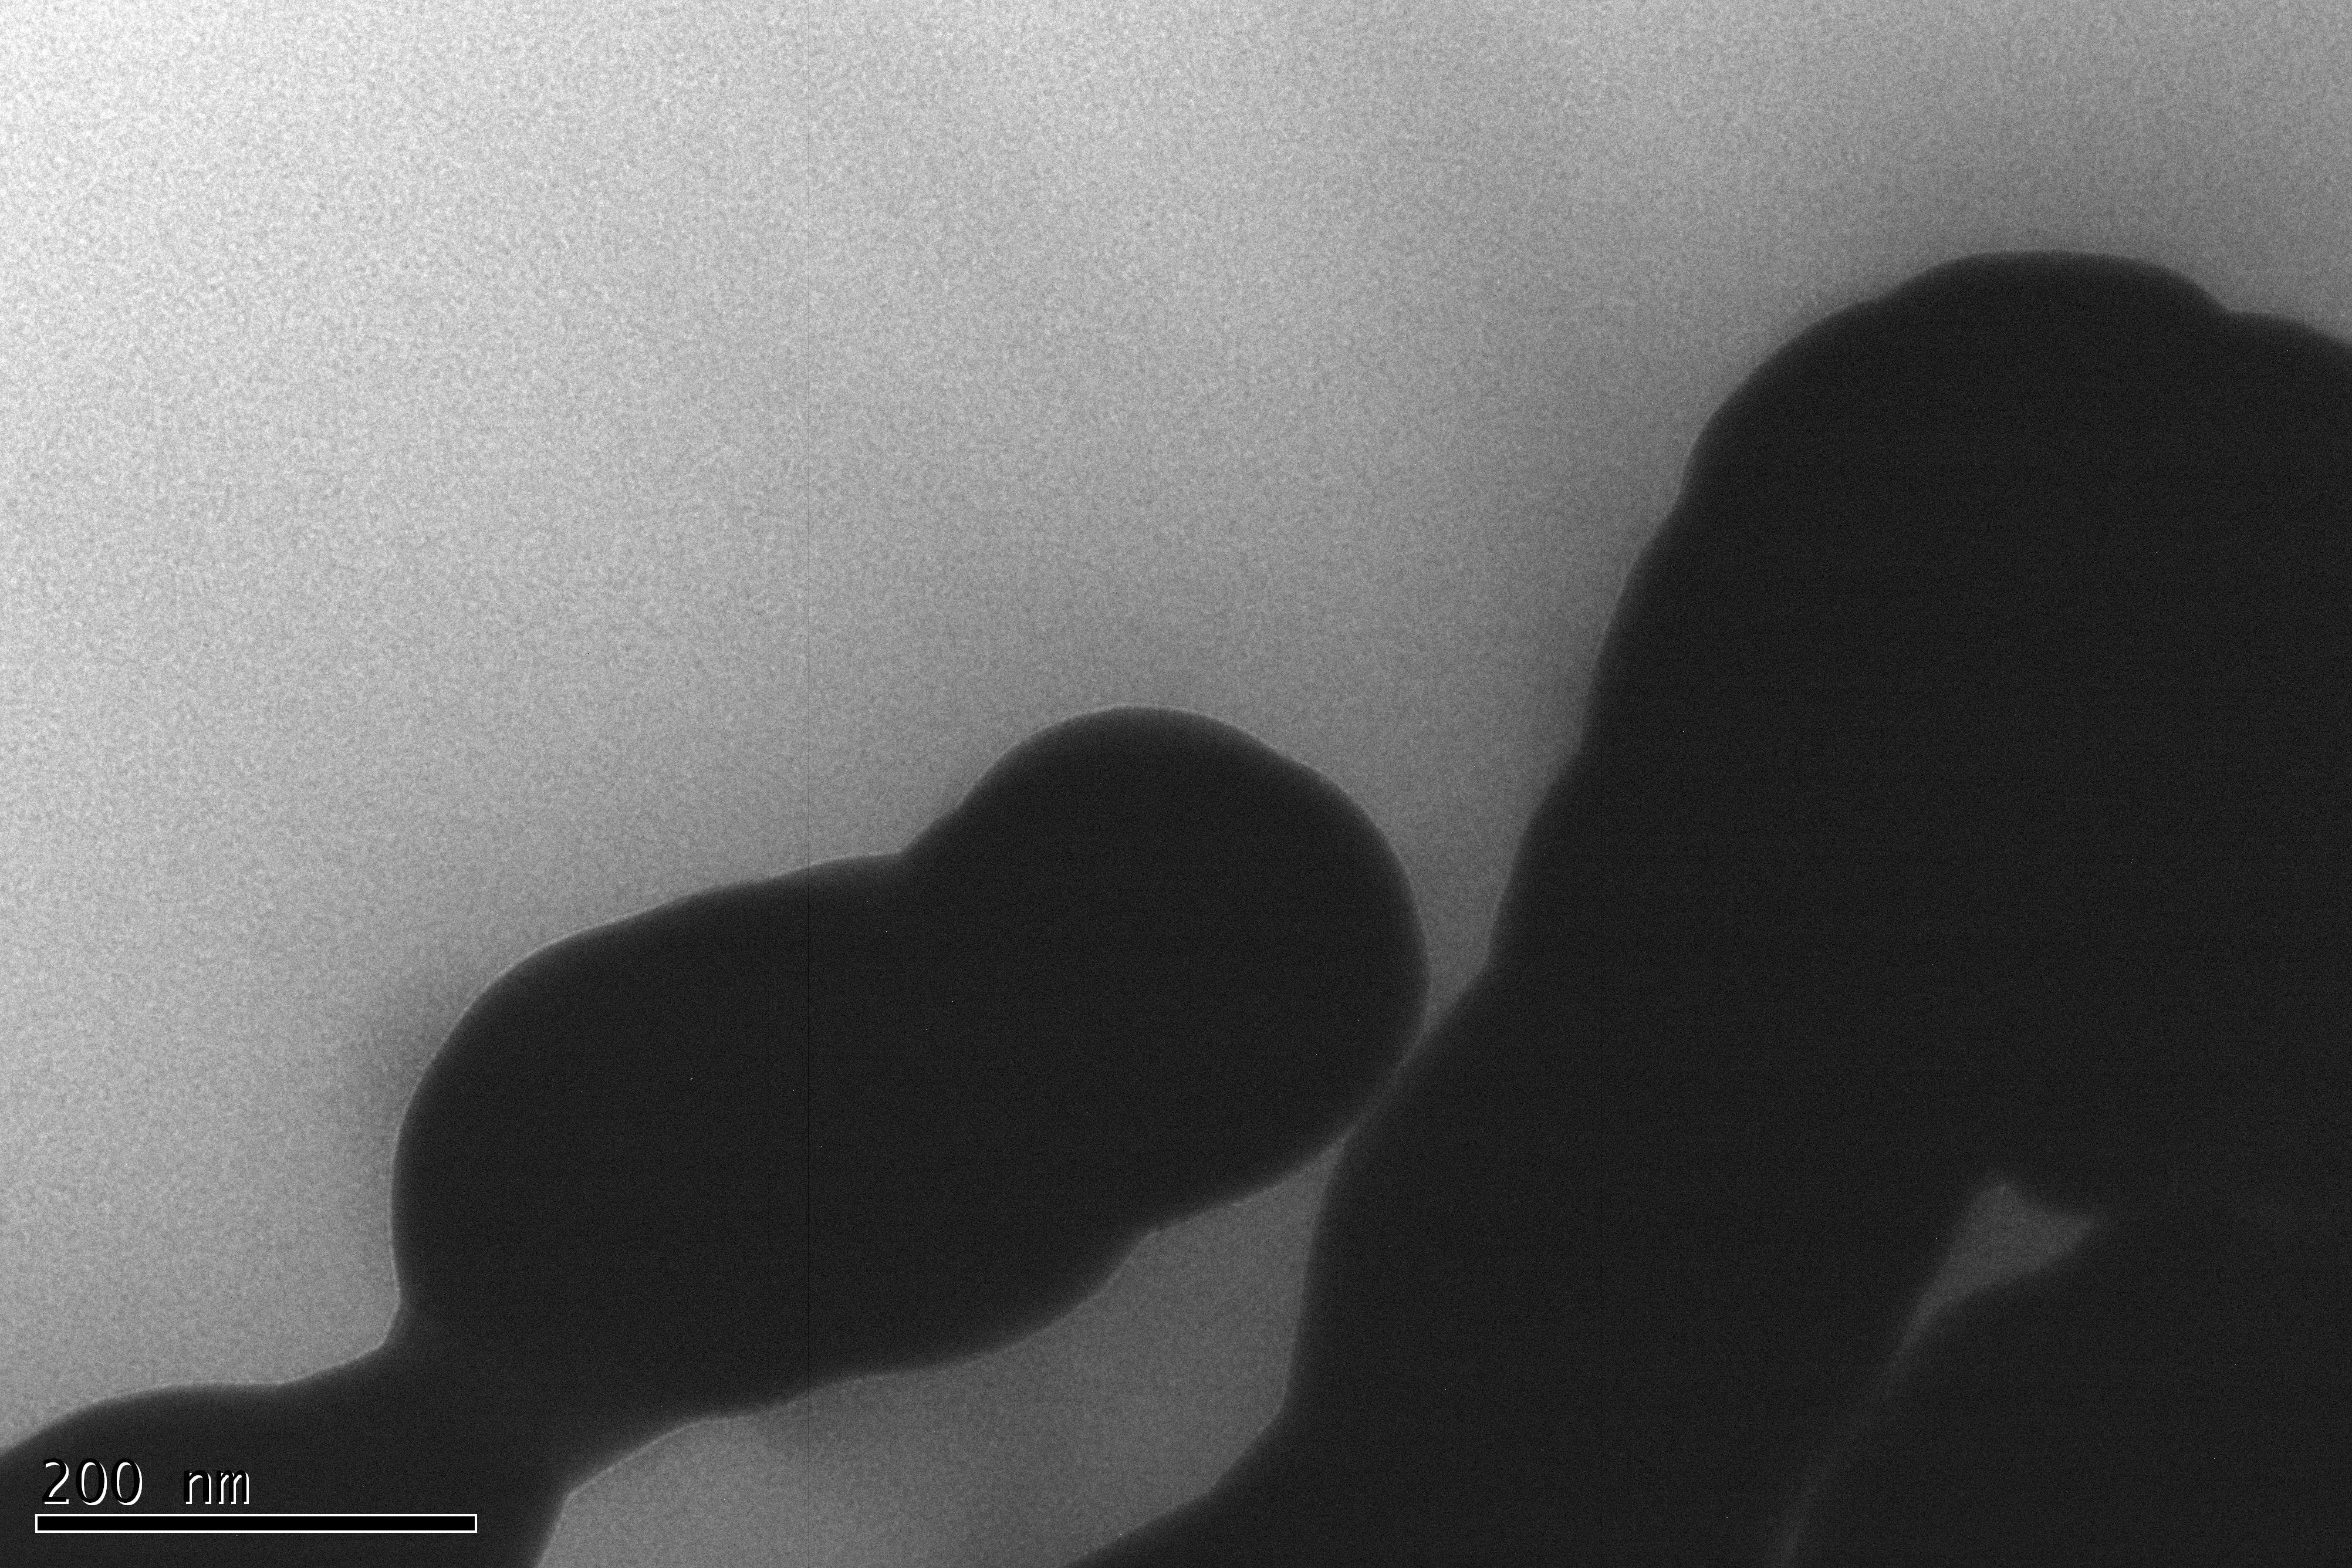
\includegraphics[width=0.6\textwidth]{Bilder/Gel-E-ZnS} 	
			\caption{TEM-Aufnahmen der Gele nach der Behandlung mit \ch{Zn[DDTC]2}.}
			\label{fig:Gel-E-ZnS}
		\end{figure}
		
		\begin{figure}[H]
			\centering
			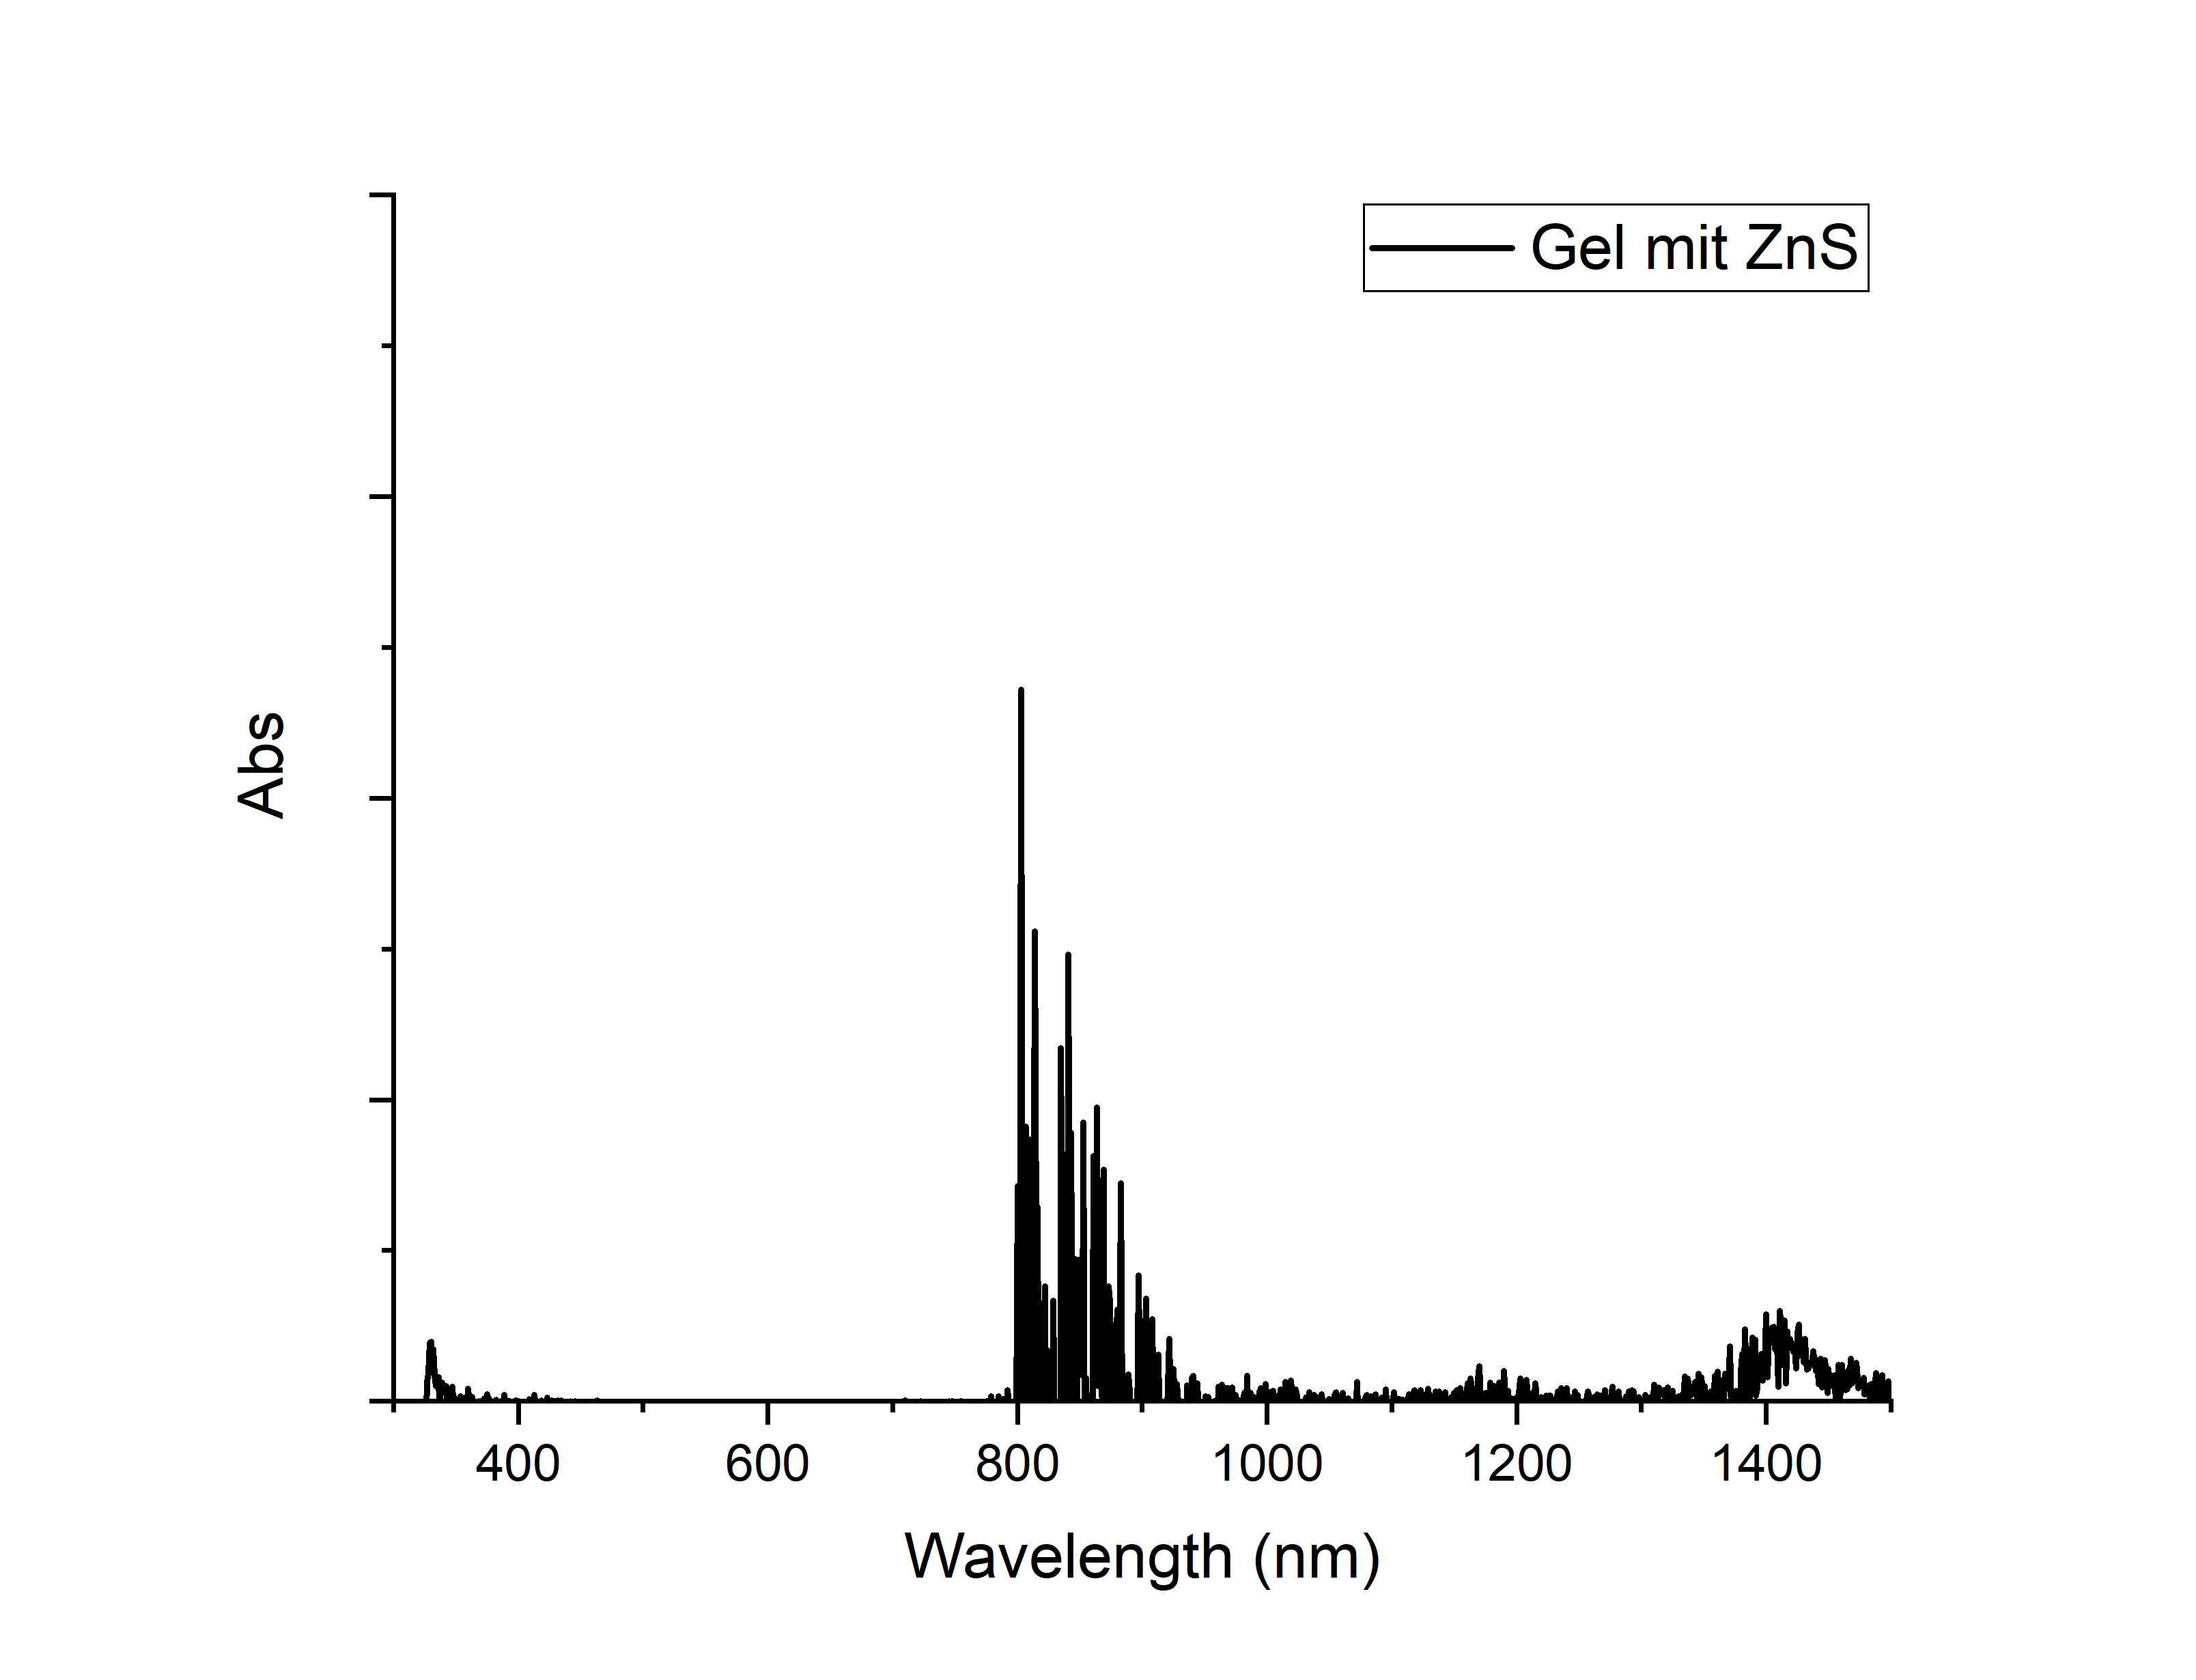
\includegraphics[width=0.6\textwidth]{Bilder/UV-Gel-E-ZnS} 	
			\caption{Absorptionsspektrum des Gels, das mit \ch{Zn[DDTC]2} behandelt wurde.}
			\label{fig:UV-Gel-E-ZnS}
		\end{figure}
	
	\subsubsection{Zusatz von Chloridionen}
	
		Da wie schon oben gezeigt, das Nukleationsverhalten durch Anwesenheit von Chlorid beeinflusst werden kann, wurde dies auch bei Anwesenheit der Gele untersucht.
		Dabei zeigten sich deutliche Unterschiede zwischen \ch{Cd[DDTC]2} und \ch{Zn[DDTC]2}.
		
		Bei den Proben die mit \ch{Cd[DDTC]2} und \ch{CdCl2} behandelt wurden verschlechterte sich das Ergebnis deutlich, wie in \cref{fig:Gel-E-CdCl} gezeigt ist.
		Die Bilder zeigen, dass das gebildete CdS nicht am Gel anliegt sondern sich überall befindet.
		Durch die Zugabe von \ch{CdCl2} scheint sich das Nukleationsverhalten so zu  ändern, dass die Partikel abgetrennt vom Gel gebildet werden, was das Verhindern des Anwachsens erklärt.  
		
		\begin{figure}[htbp]
			\centering
			\subfloat[\label{fig:Gel-E-CdCl-1-1}]{%
				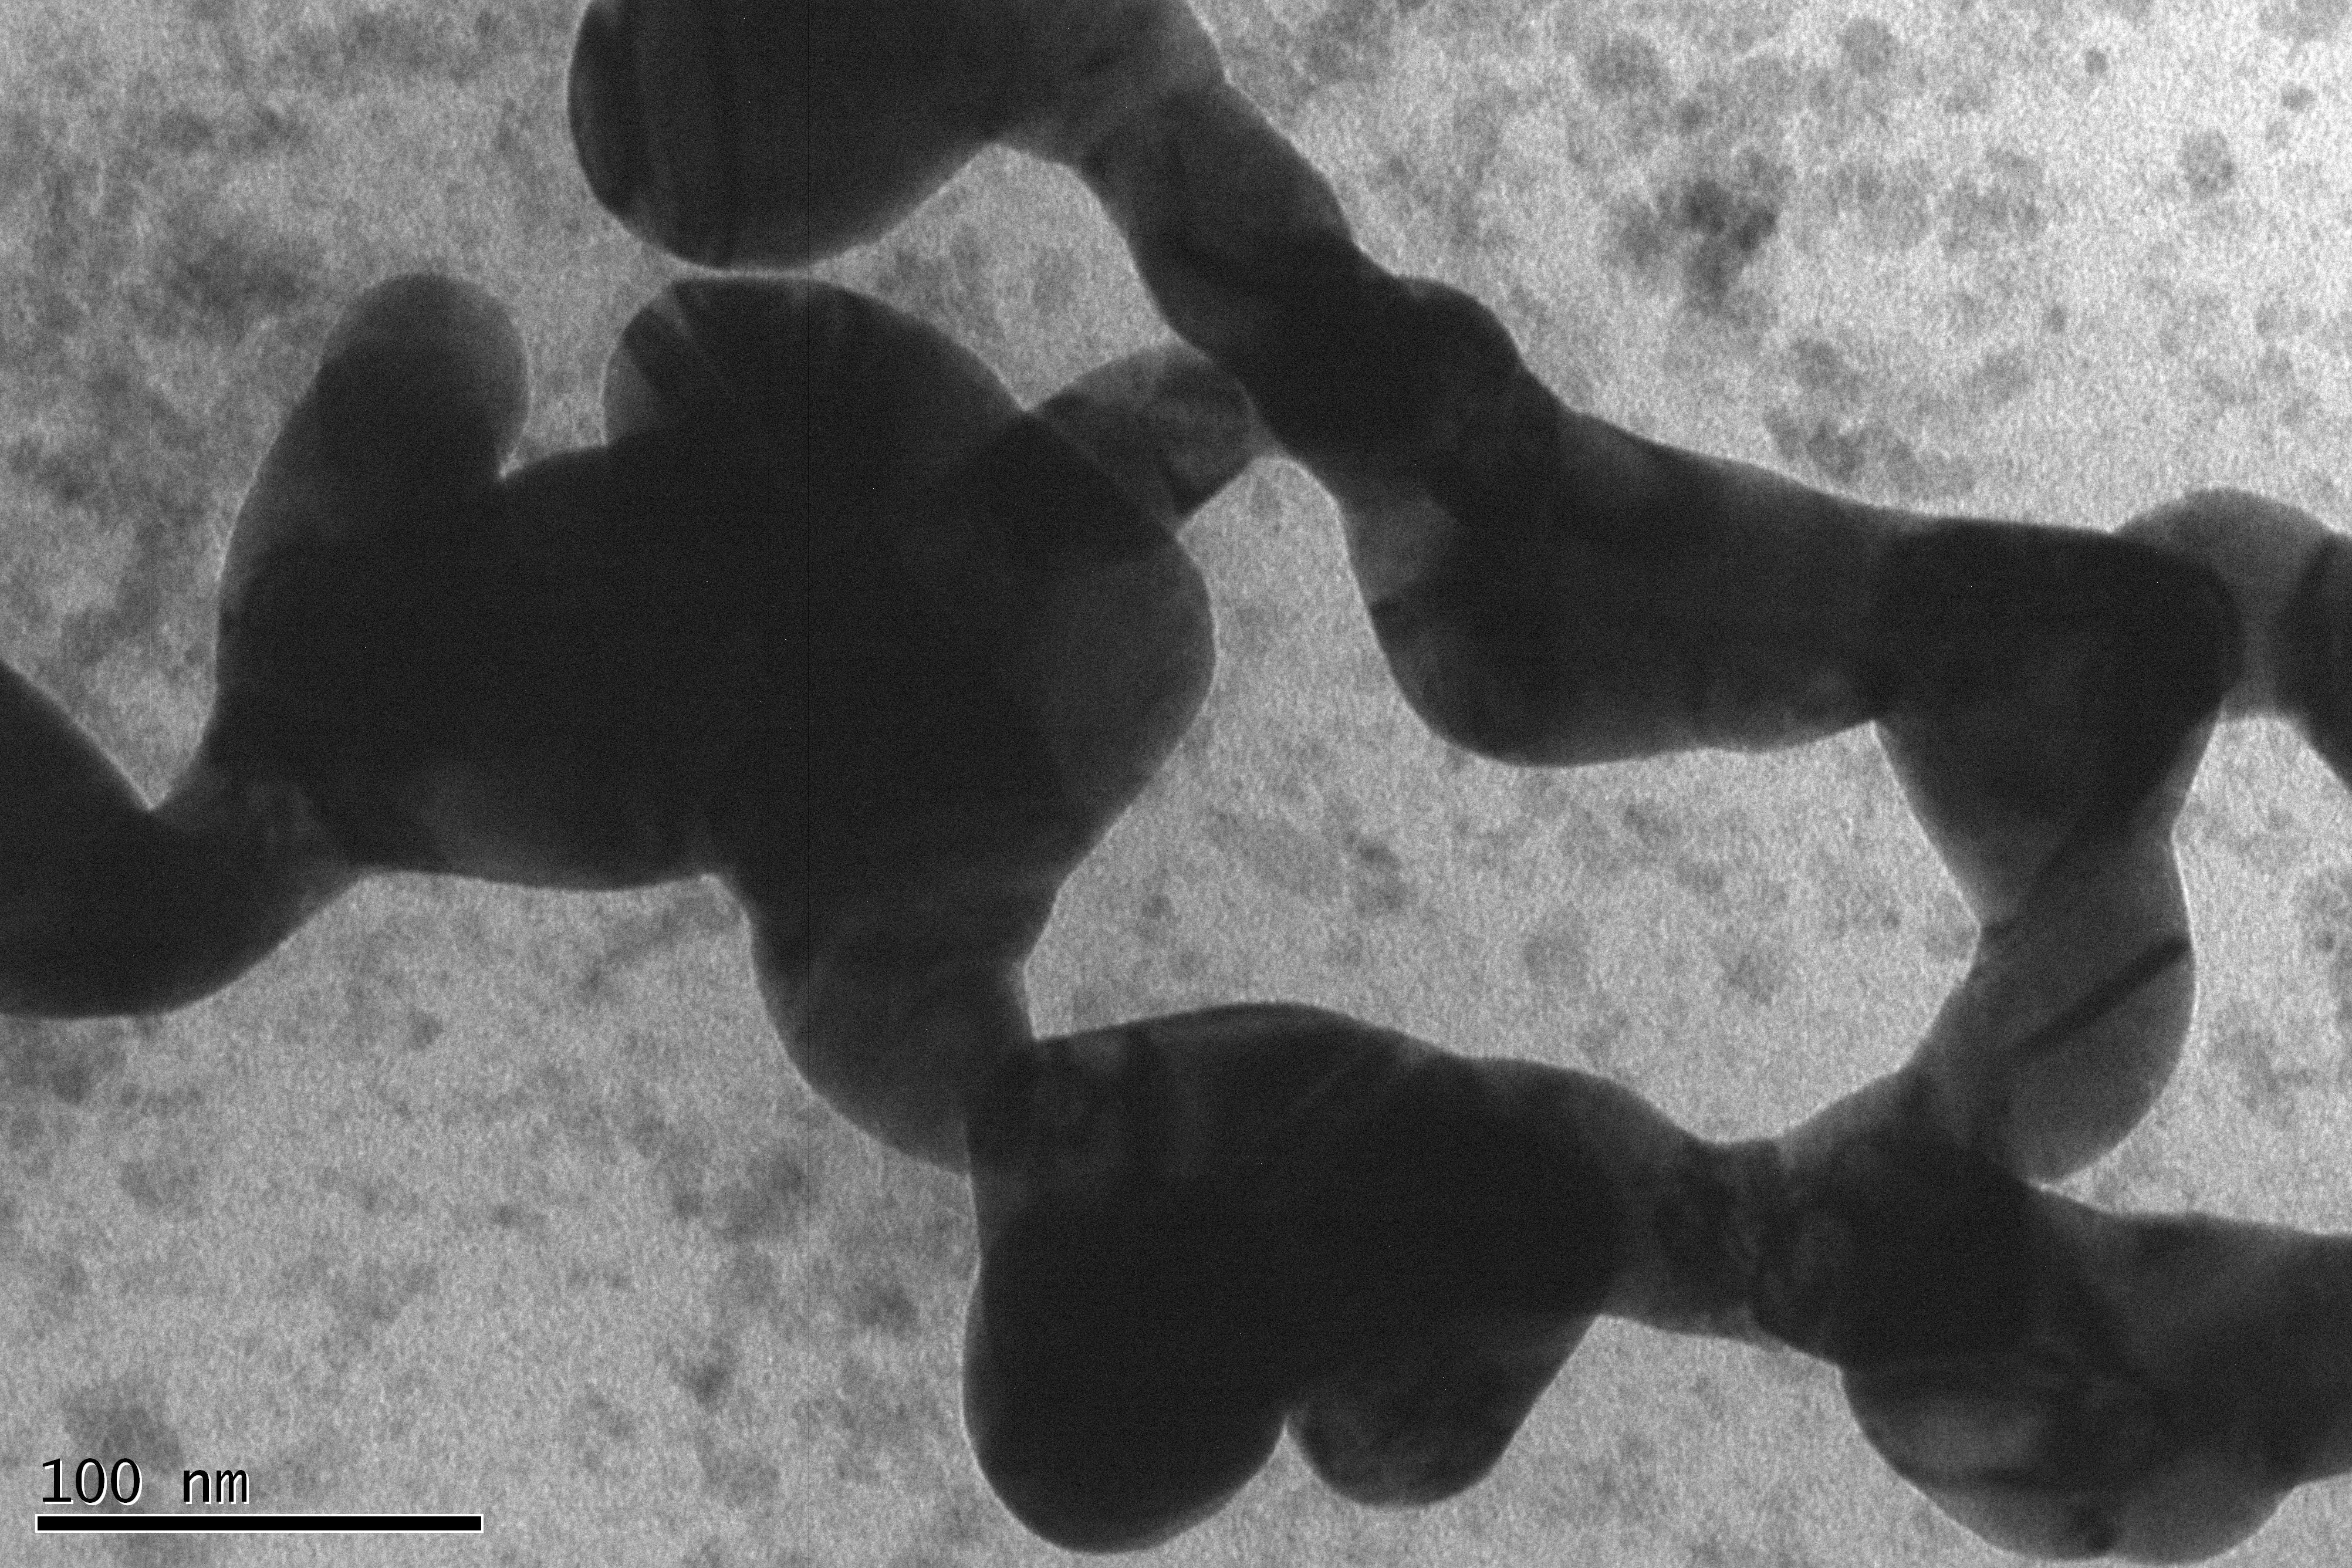
\includegraphics[width=0.33\linewidth]{Bilder/Gel-E-CdCl-1-1}}
			\subfloat[\label{fig:Gel-E-CdCl-1-4}]{%
				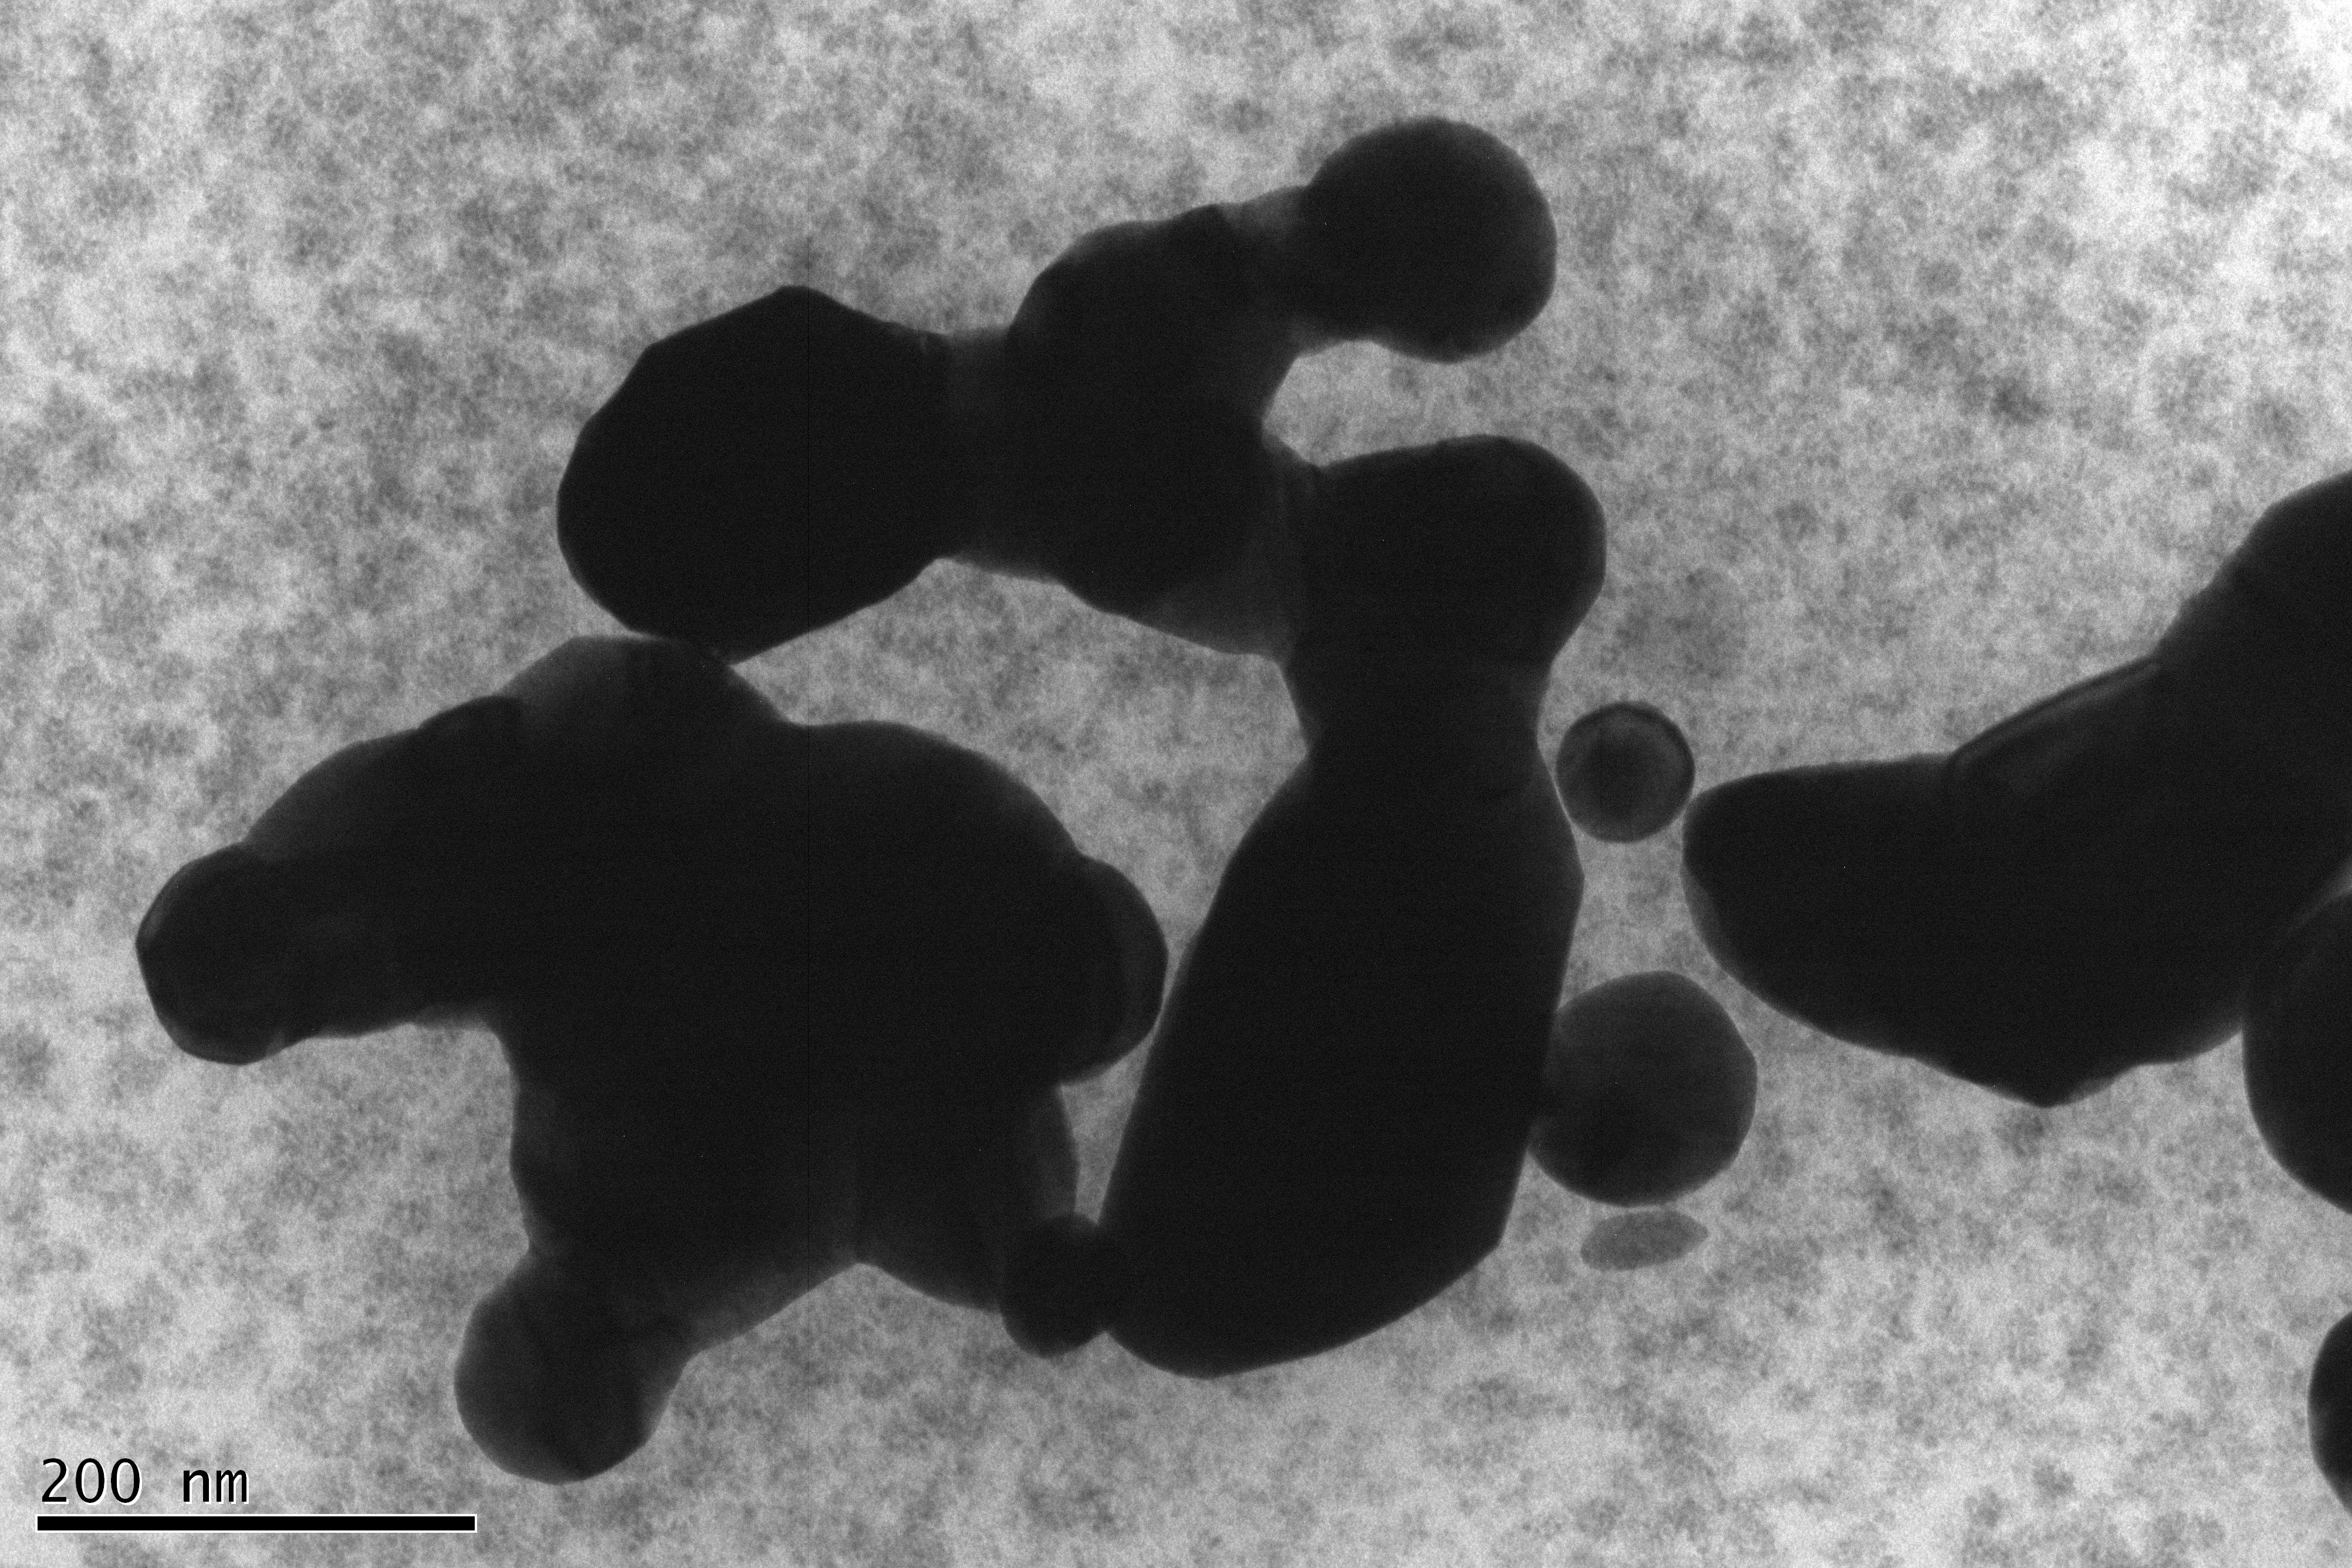
\includegraphics[width=0.33\linewidth]{Bilder/Gel-E-CdCl-1-4}}
			\subfloat[\label{fig:Gel-E-CdCl-1-10}]{%
				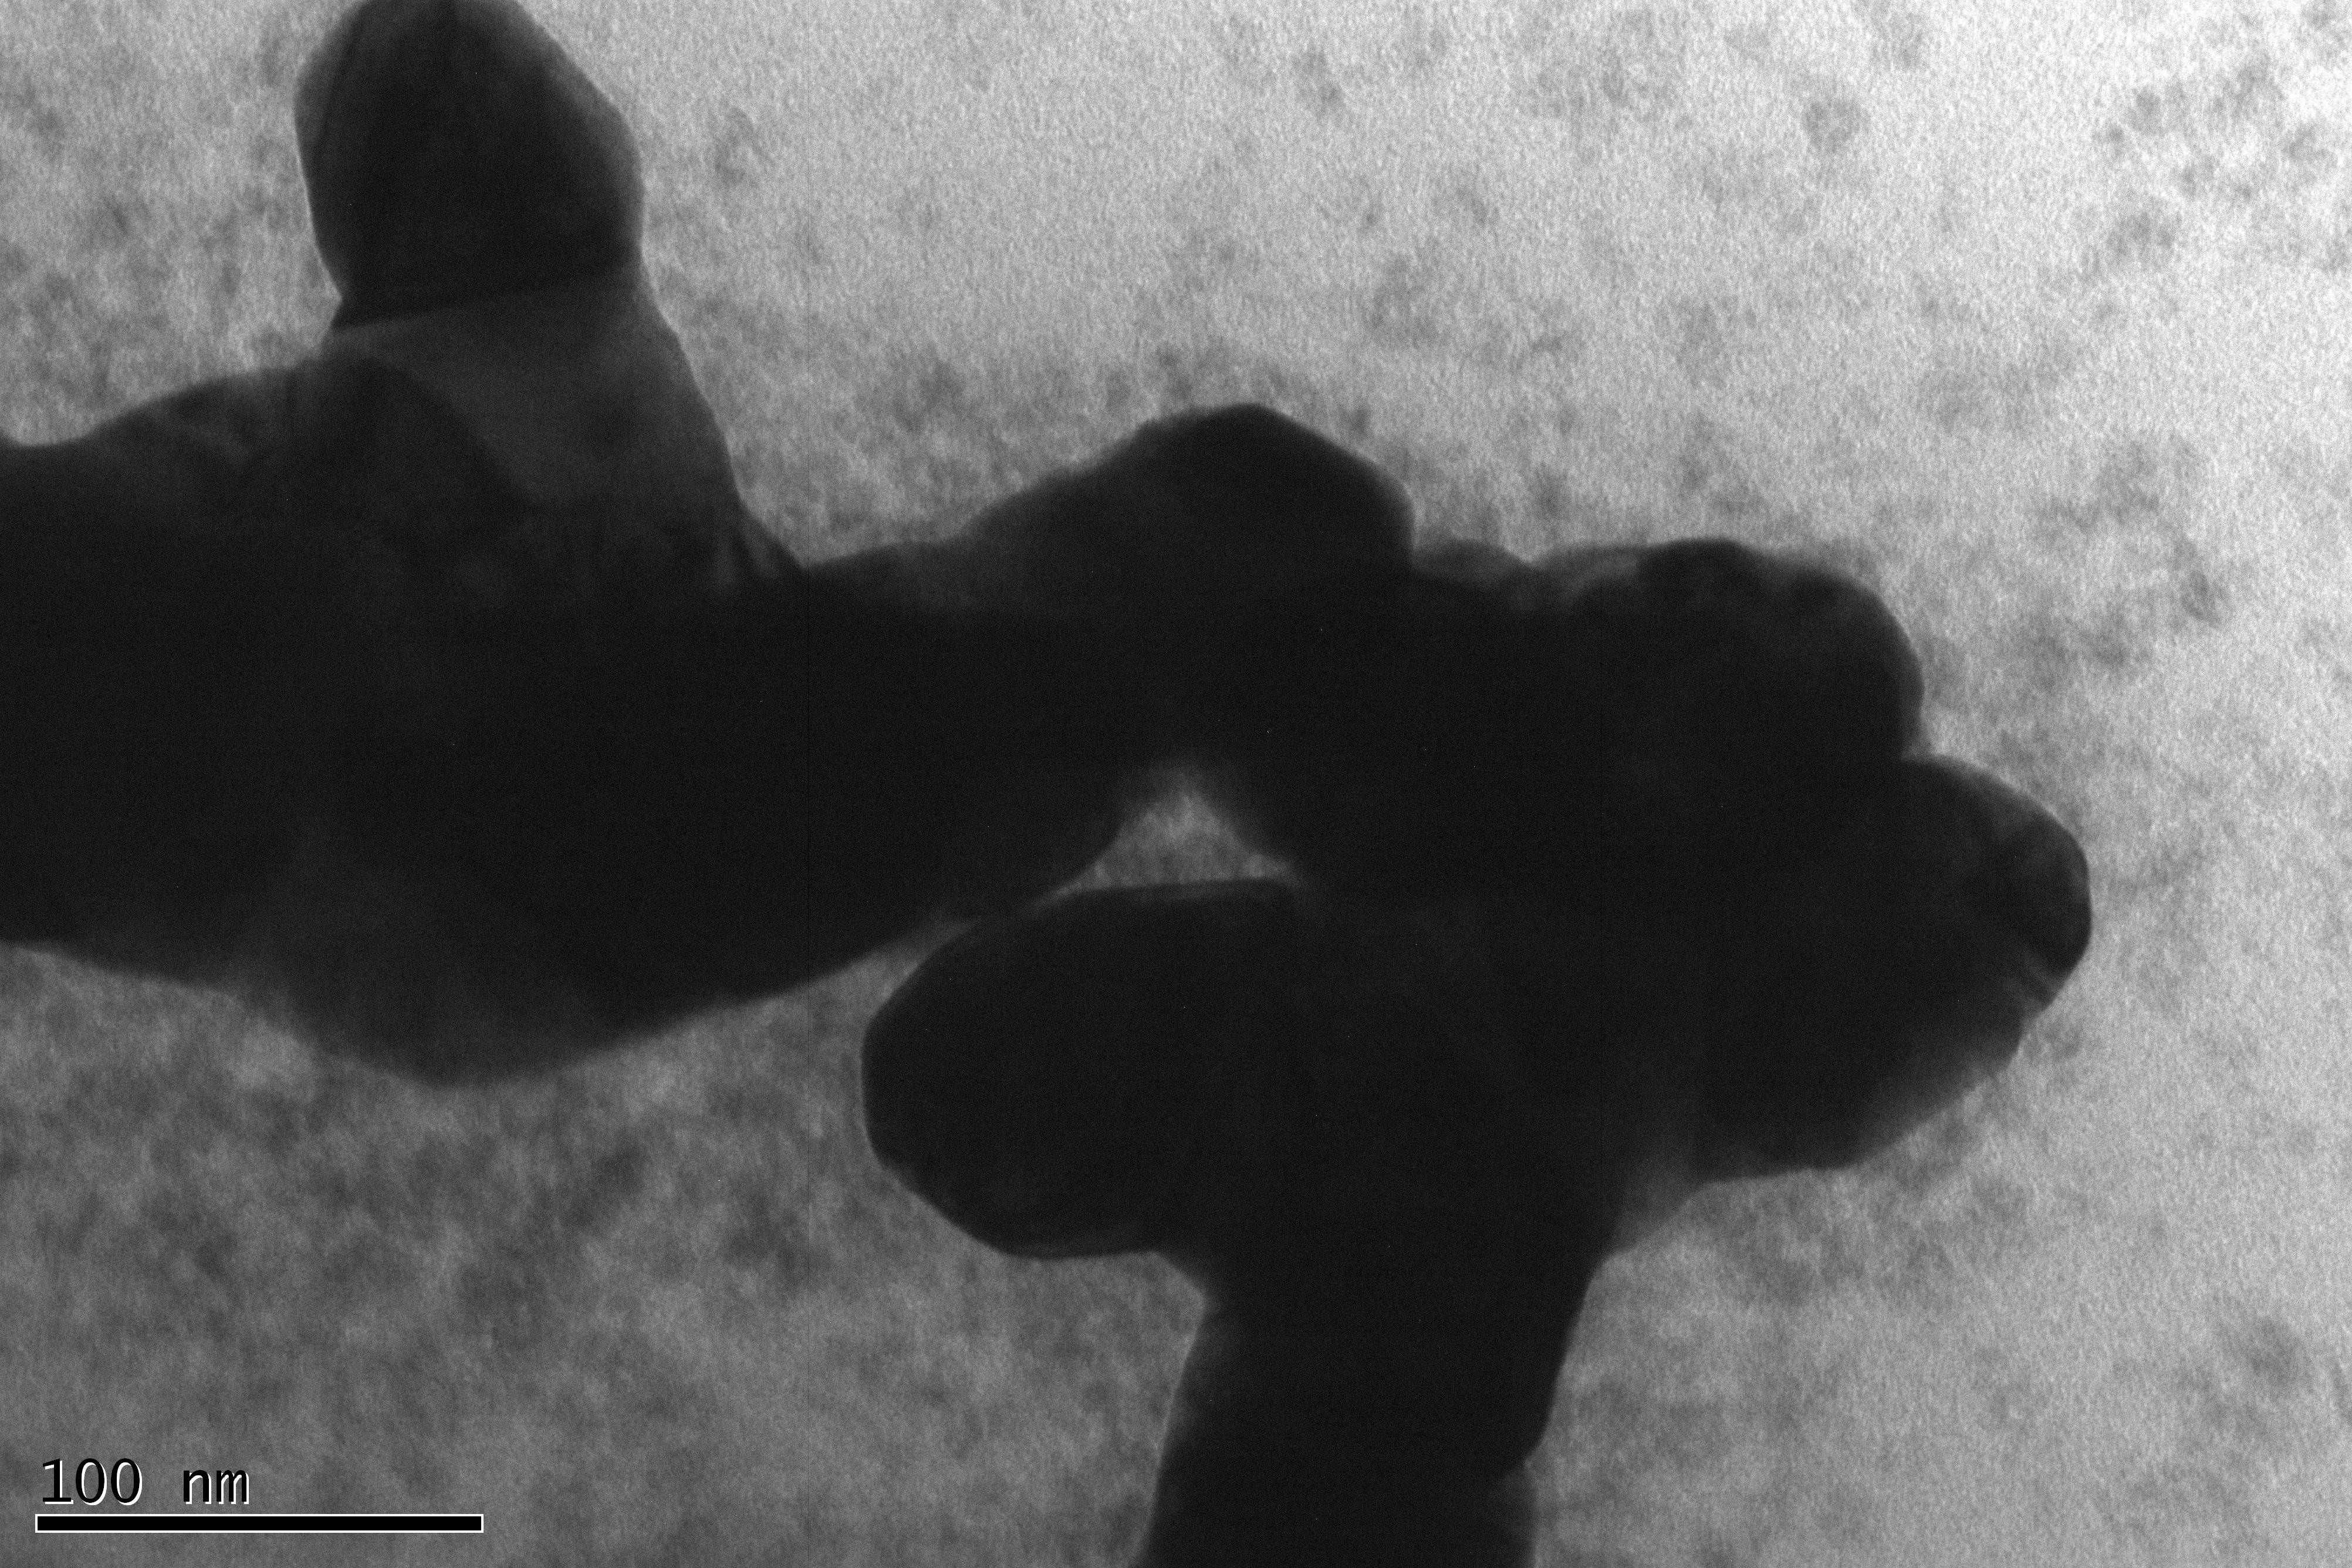
\includegraphics[width=0.33\linewidth]{Bilder/Gel-E-CdCl-1-10}}
			\caption{TEM-Aufnahmen der Gele, die mit \ch{Cd[DDTC]2} und \ch{CdCl2} im Verhältnis \emph{(a)}: 1:1; \emph{(b)}: 1:4; \emph{(c)}: 1:10 \ch{Cd[DDTC]2} zu \ch{CdCl2} behandelt wurden.}
			\label{fig:Gel-E-CdCl}
		\end{figure}
		
		Bei den Proben die mit \ch{Zn[DDTC]2} und \ch{ZnCl2} behandelt wurden ließ sich etwas anderes beobachten.
		Während hier keine Partikelbildung bei reinem \ch{Zn[DDTC]2} zu erkennen war, konnte dies durch Zugabe vom \ch{ZnCl2} verändert werden.
		Bei den Proben, die im Verhältnis 1:1 (\cref{fig:Gel-E-ZnCl-1-1})und 1:10 (\cref{fig:Gel-E-ZnCl-1-10}) \ch{Zn[DDTC]2} zu \ch{ZnCl2} behandelt wurden, konnte an einigen Stellen die Ausbildung von einer dünnen Schicht an den Gelen beobachtet werden.
		Bei der Probe im 1:10 Verhältnis konnte dabei sogar eine komplette Hülle um einige Teile des Gels beobachtet werden, was besonders gut in \cref{fig:Gel-E-ZnCl-1-10_1} zu erkennen ist.
		
		\begin{figure}[htbp]
			\centering
			\subfloat[\label{fig:Gel-E-ZnCl-1-1_1}]{%
				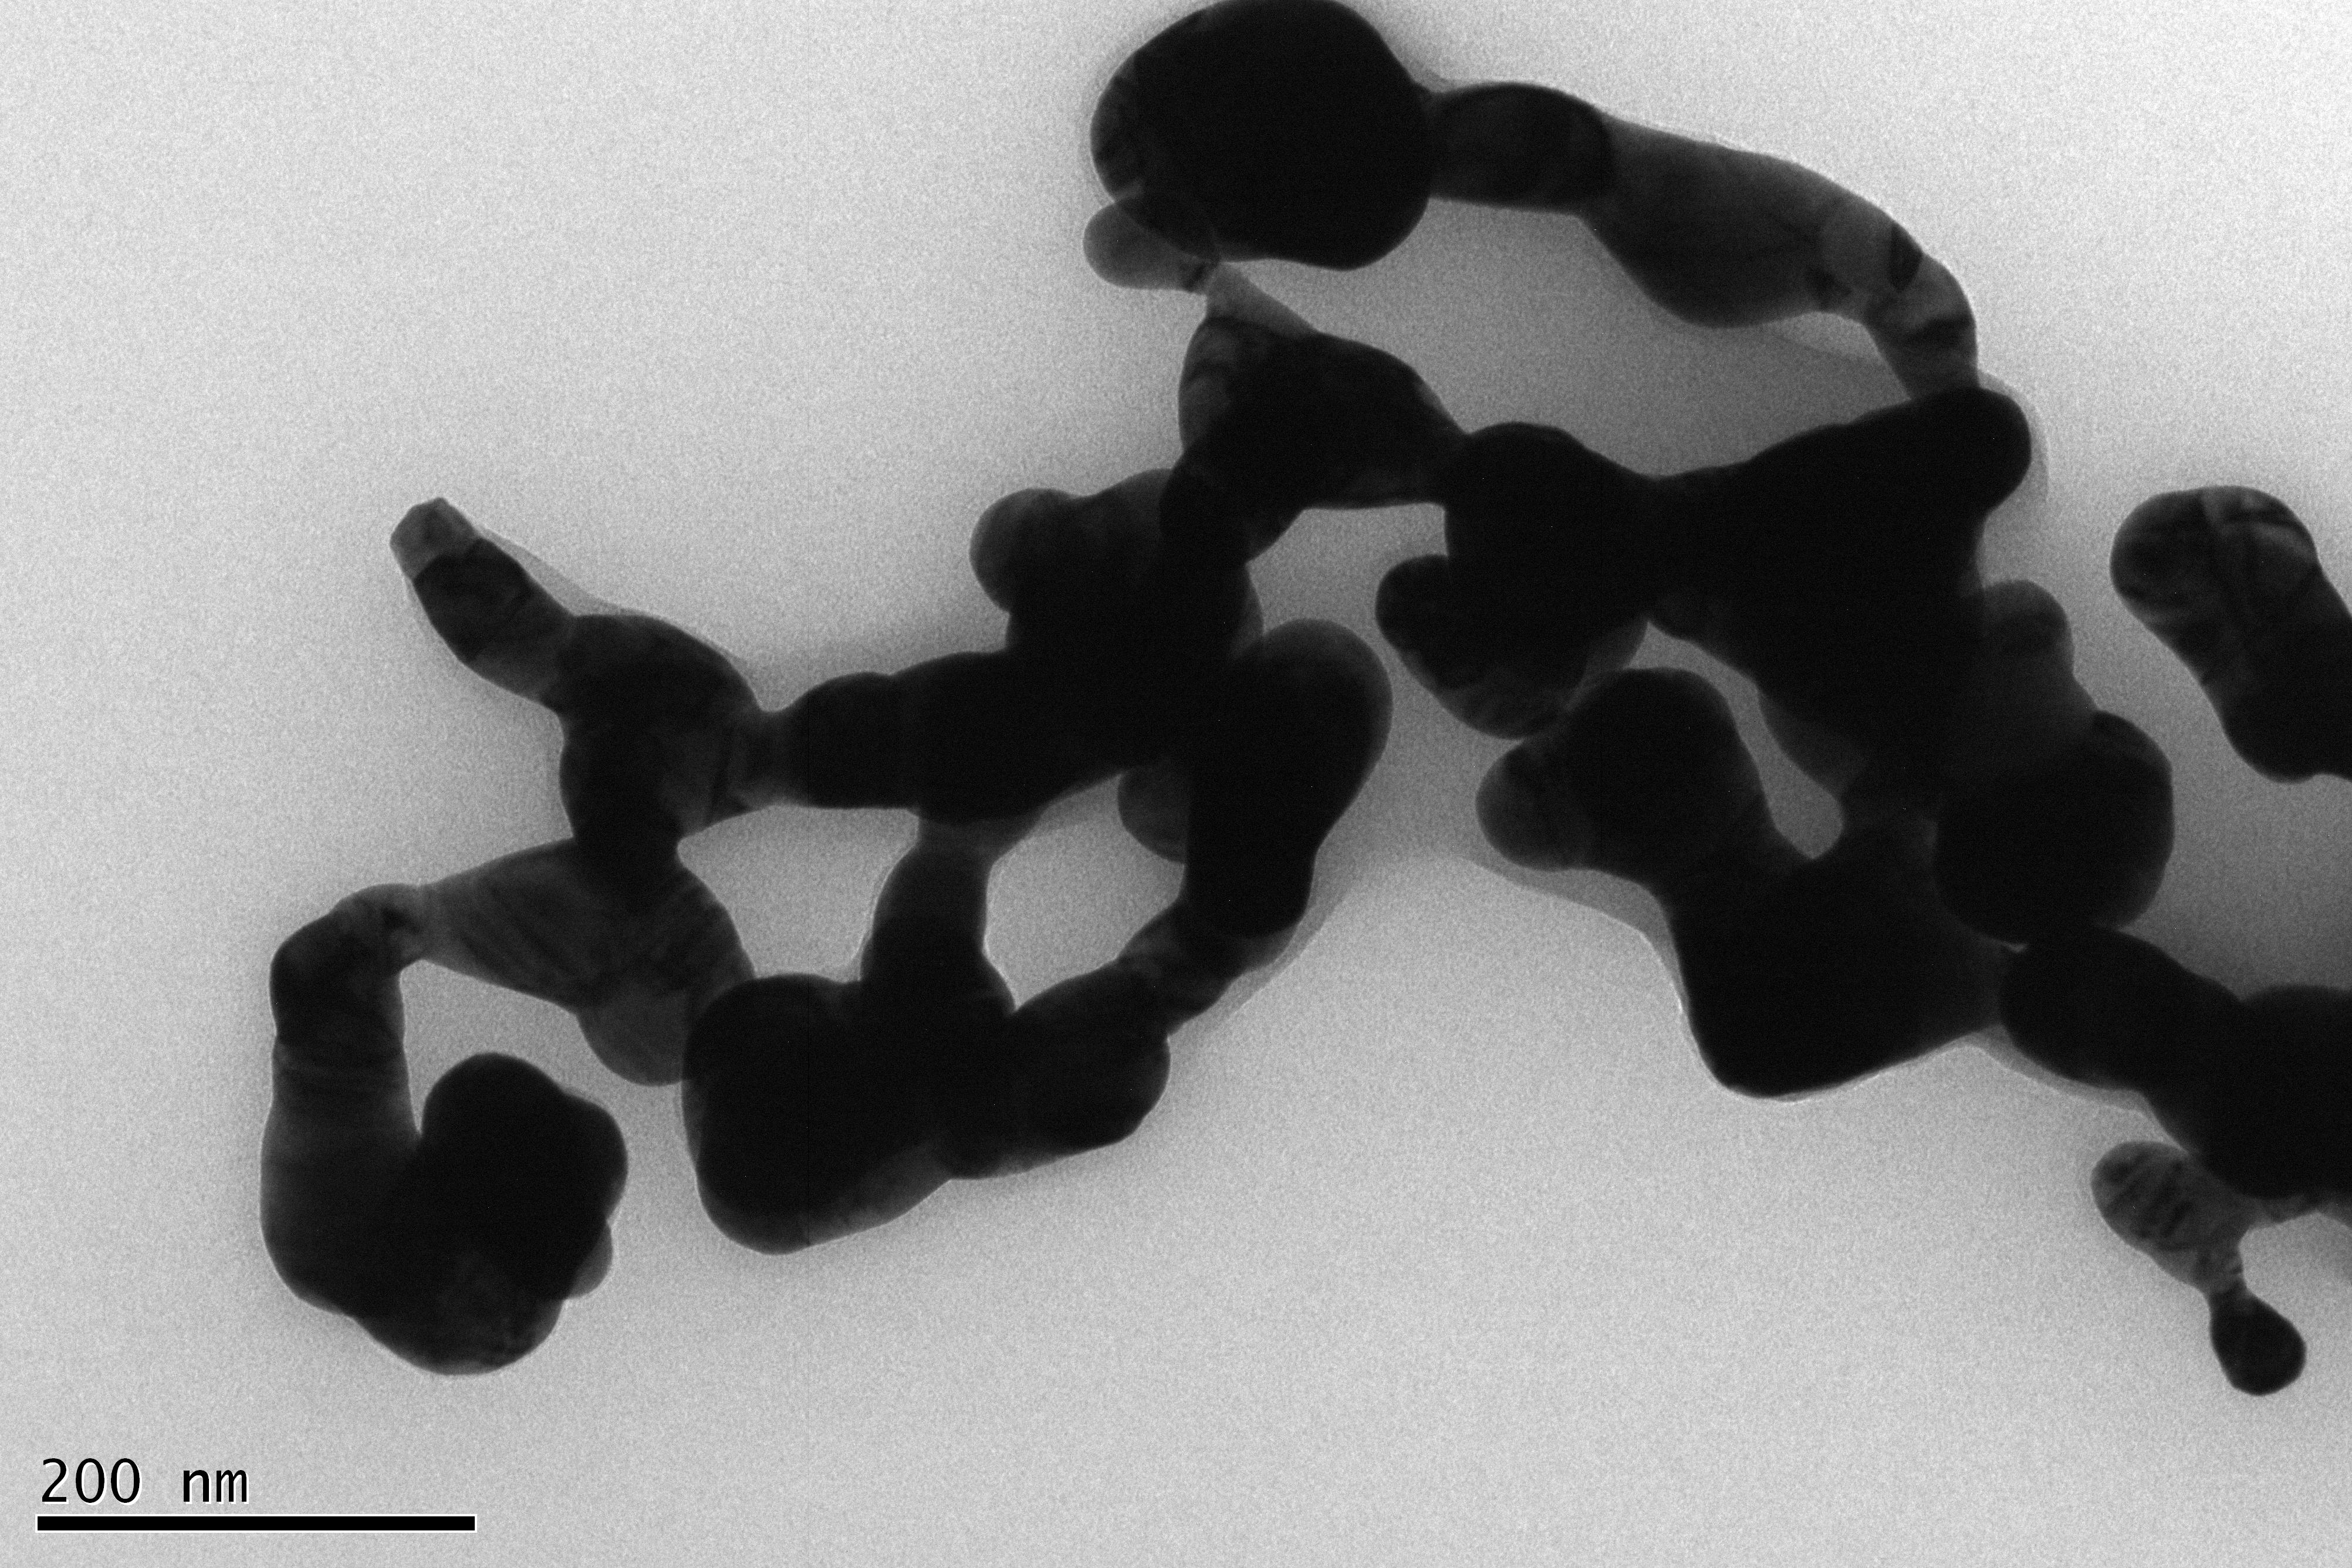
\includegraphics[width=0.33\linewidth]{Bilder/Gel-E-ZnCl-1-1_1}}
			\subfloat[\label{fig:Gel-E-ZnCl-1-1_2}]{%
				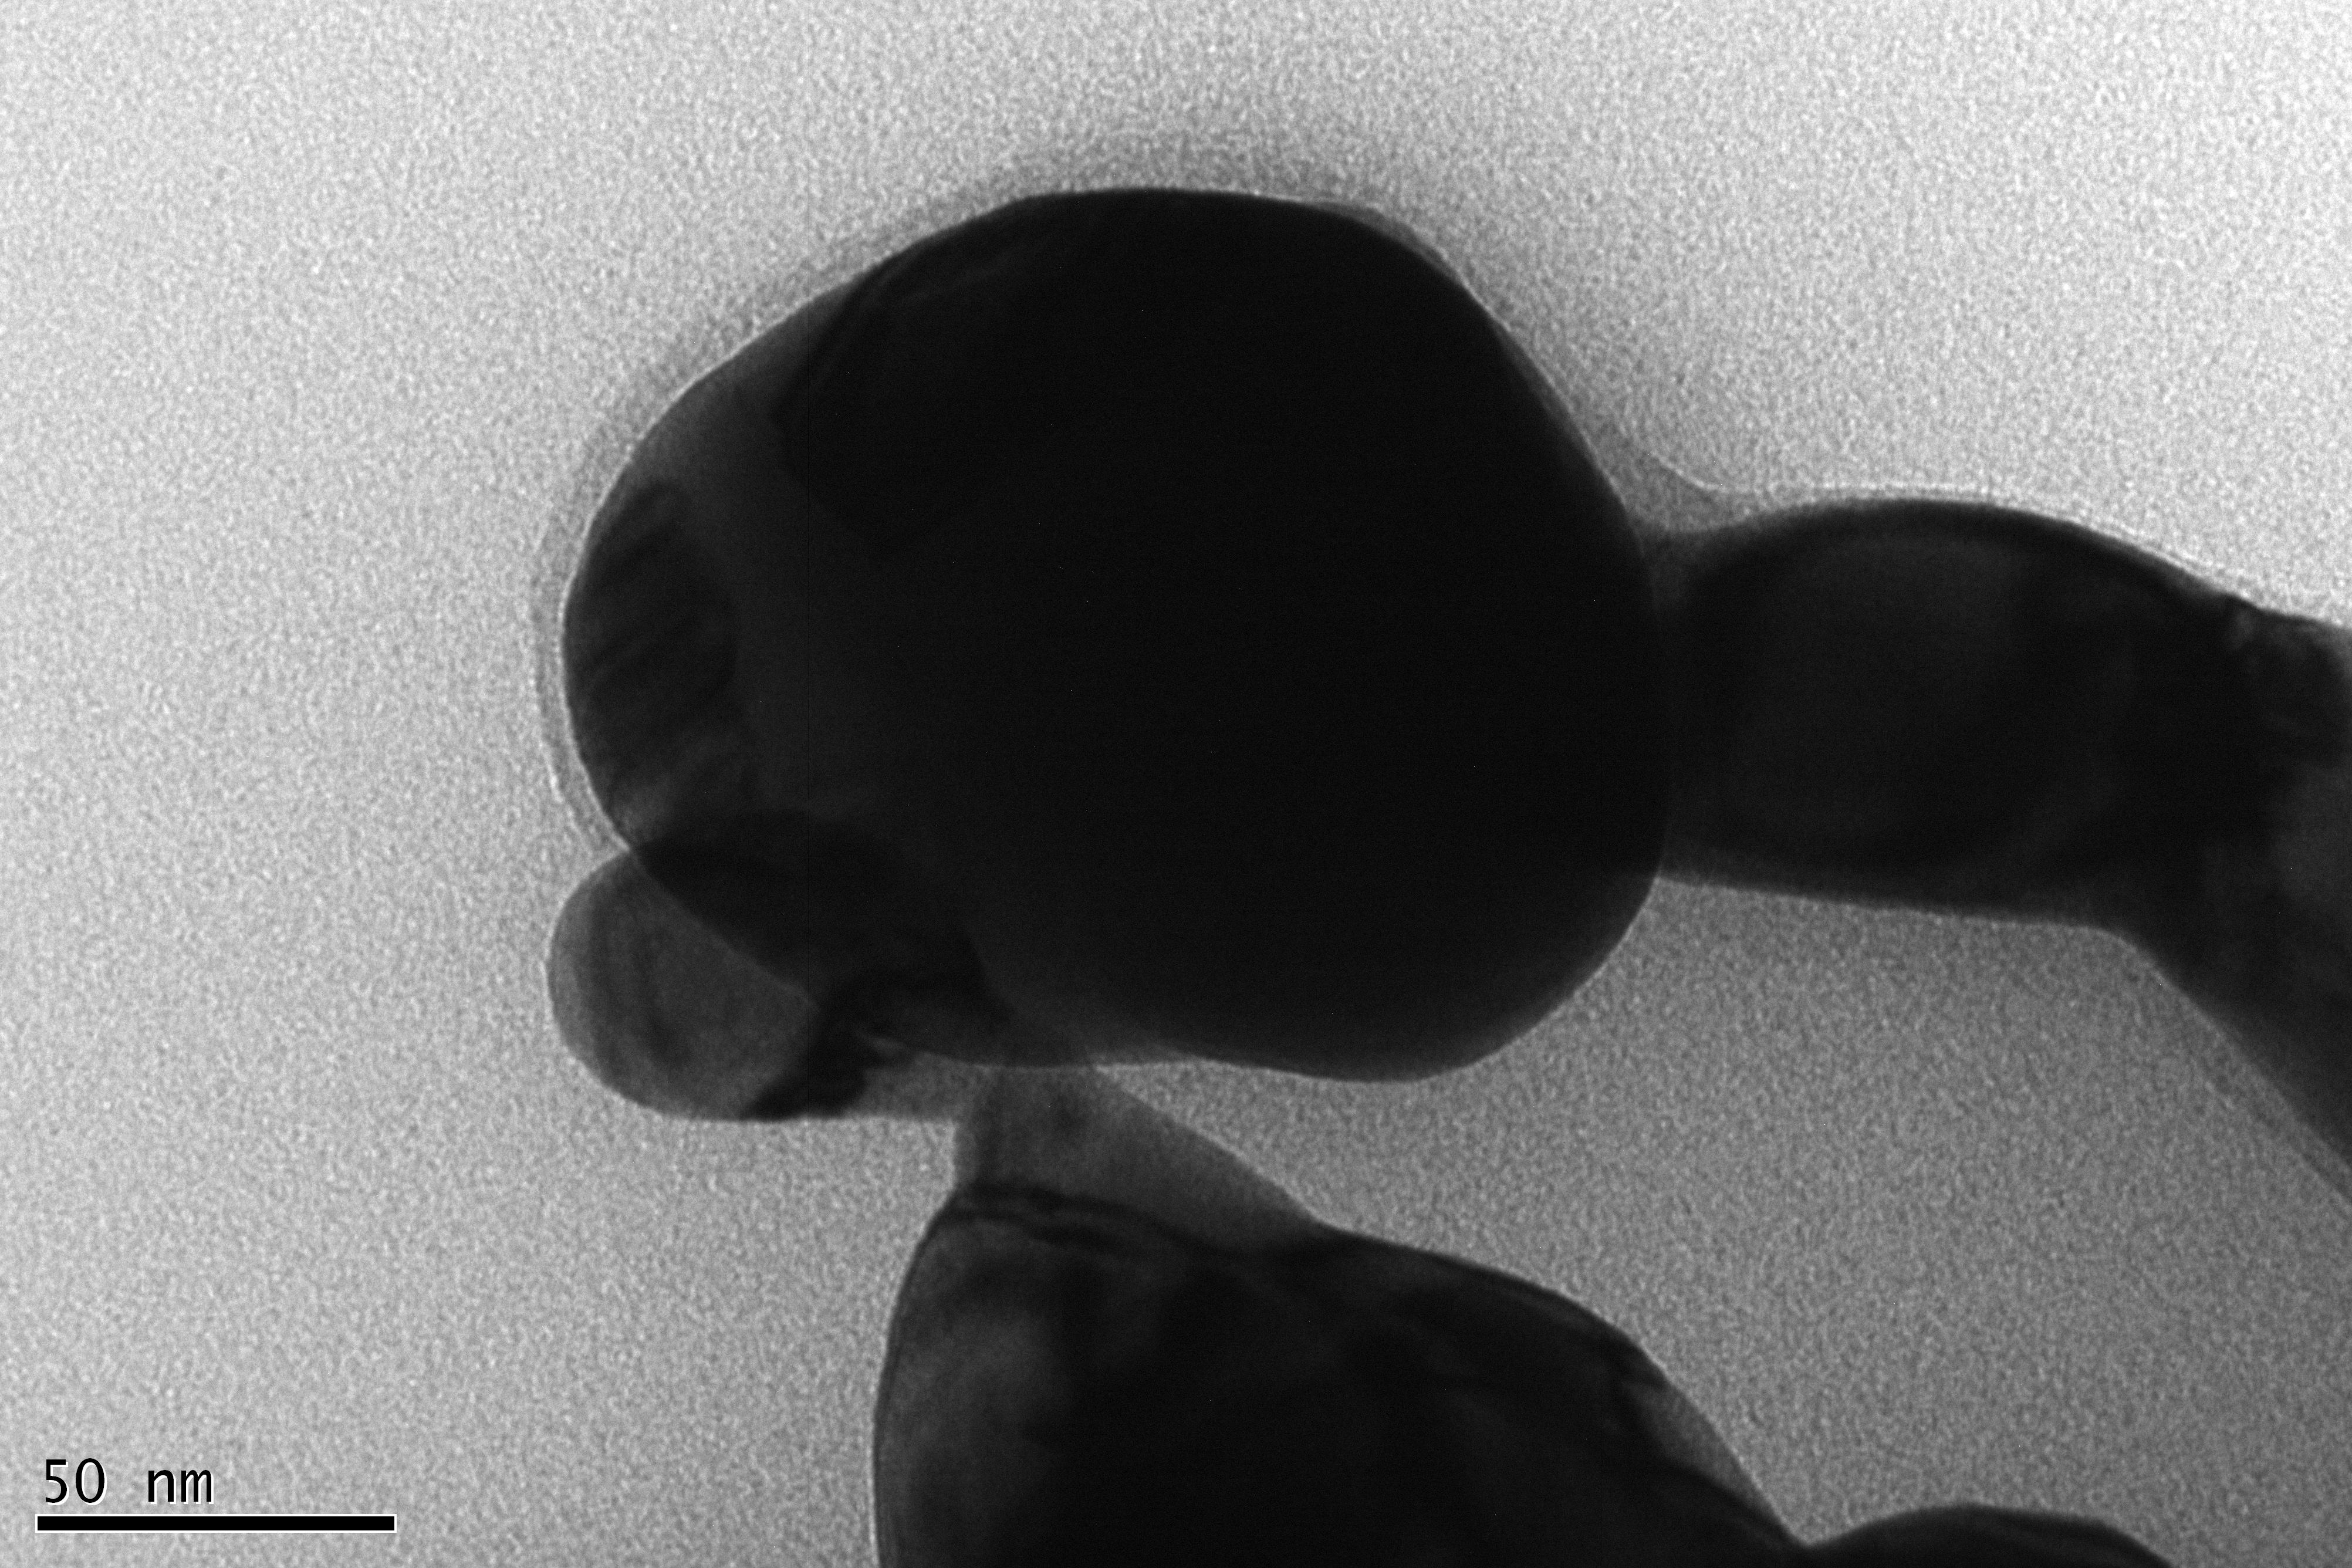
\includegraphics[width=0.33\linewidth]{Bilder/Gel-E-ZnCl-1-1_2}}
			\subfloat[\label{fig:Gel-E-ZnCl-1-1_3}]{%
				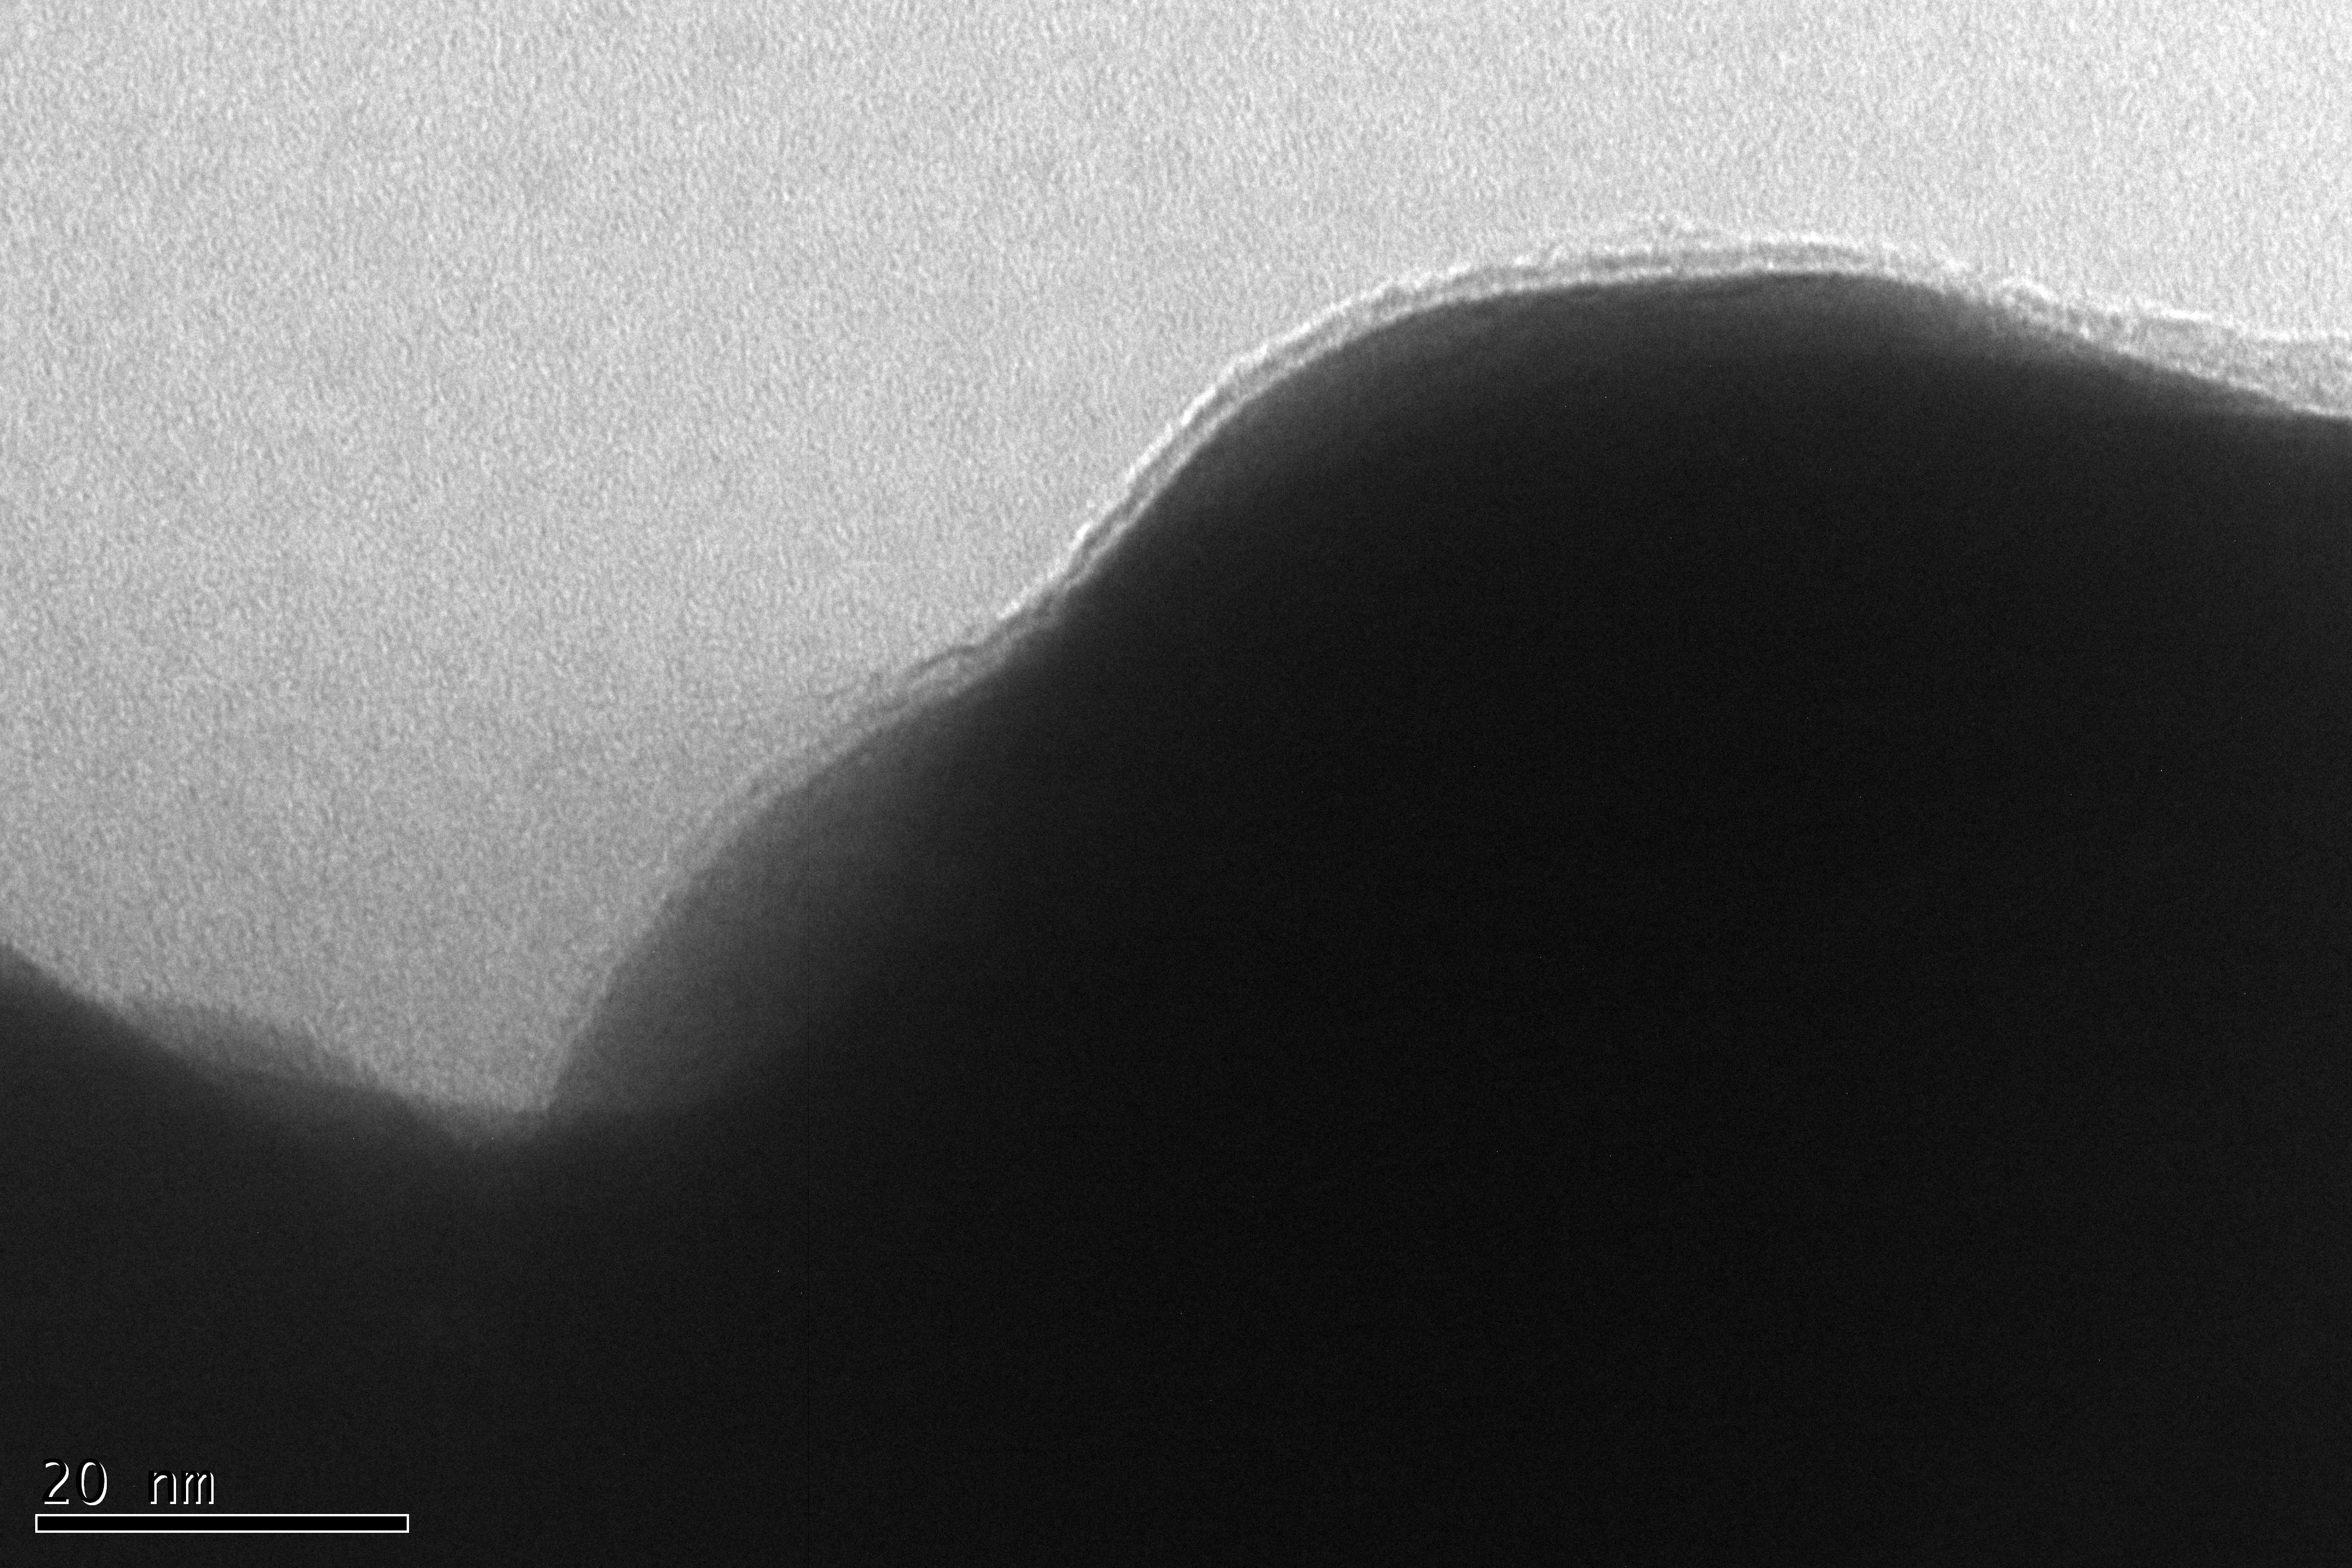
\includegraphics[width=0.33\linewidth]{Bilder/Gel-E-ZnCl-1-1_3}}
			\caption{TEM-Aufnahmen des Gels, das mit \ch{Zn[DDTC]2} und \ch{ZnCl2} im Verhältnis 1:1 \ch{Zn[DDTC]2} zu \ch{ZnCl2} behandelt wurde.}
			\label{fig:Gel-E-ZnCl-1-1}
		\end{figure}
		
		\begin{figure}[htbp]
			\centering
			\subfloat[\label{fig:Gel-E-ZnCl-1-10_1}]{%
				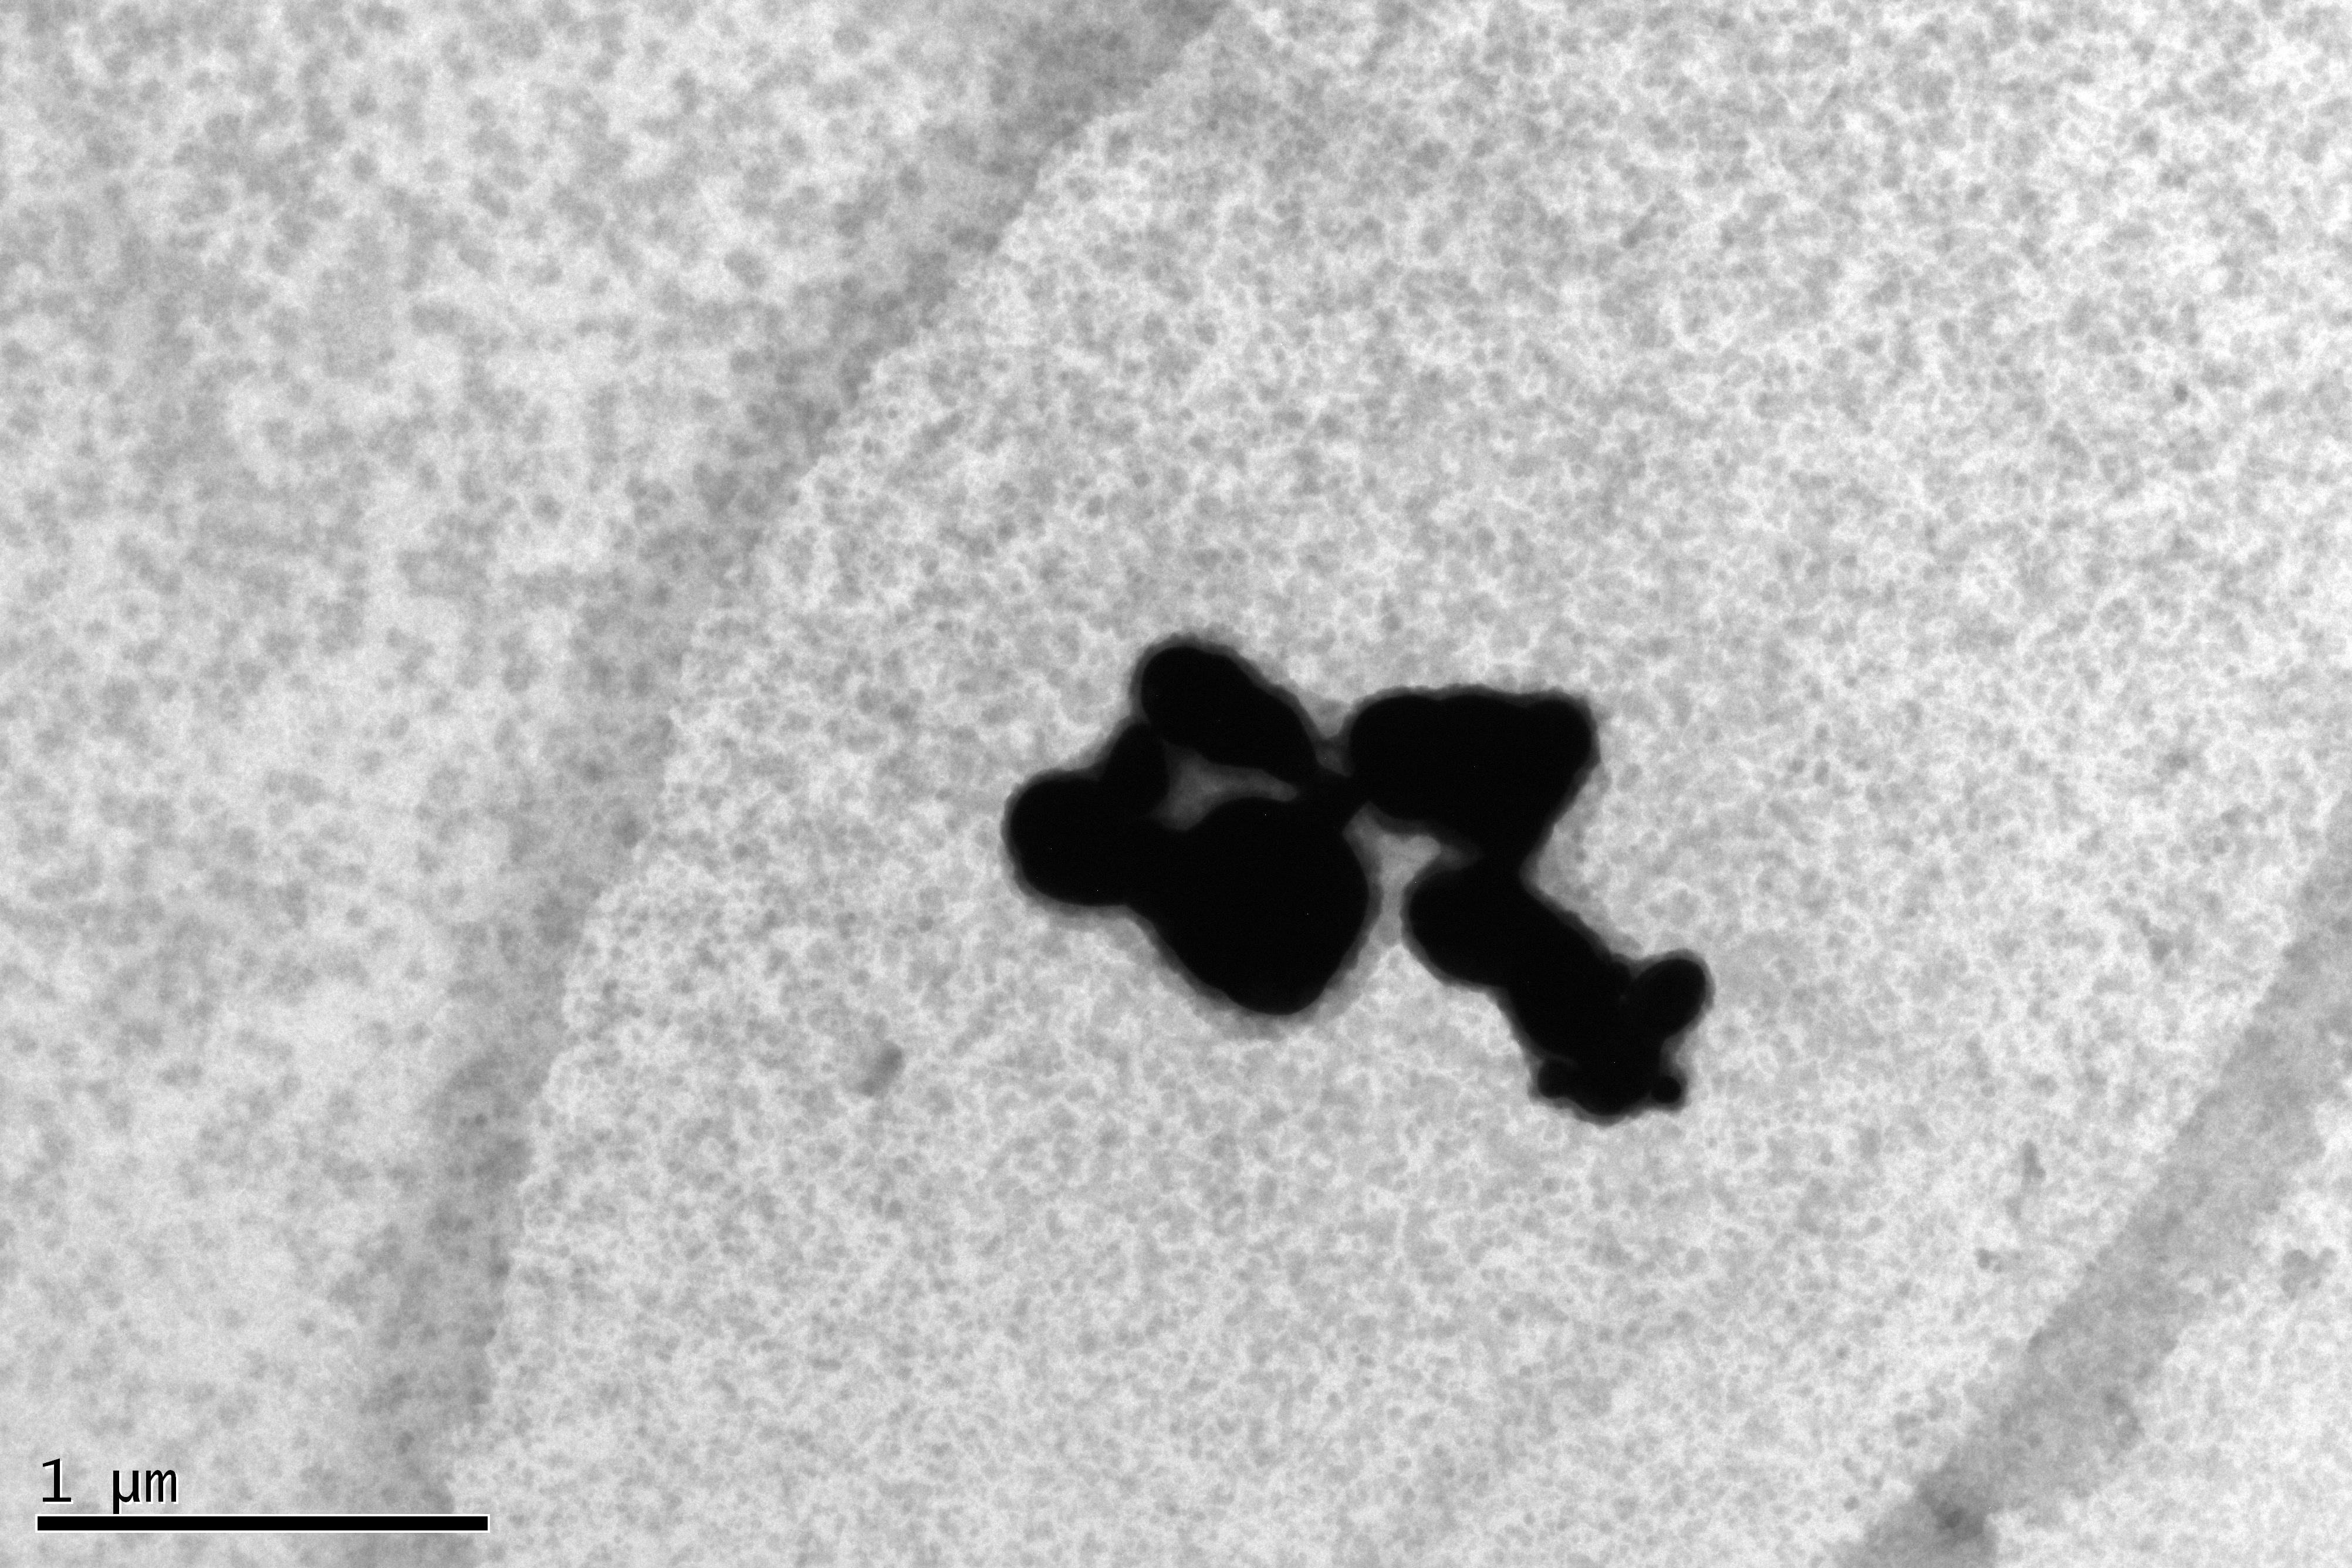
\includegraphics[width=0.33\linewidth]{Bilder/Gel-E-ZnCl-1-10_1}}
			\subfloat[\label{fig:Gel-E-ZnCl-1-10_2}]{%
				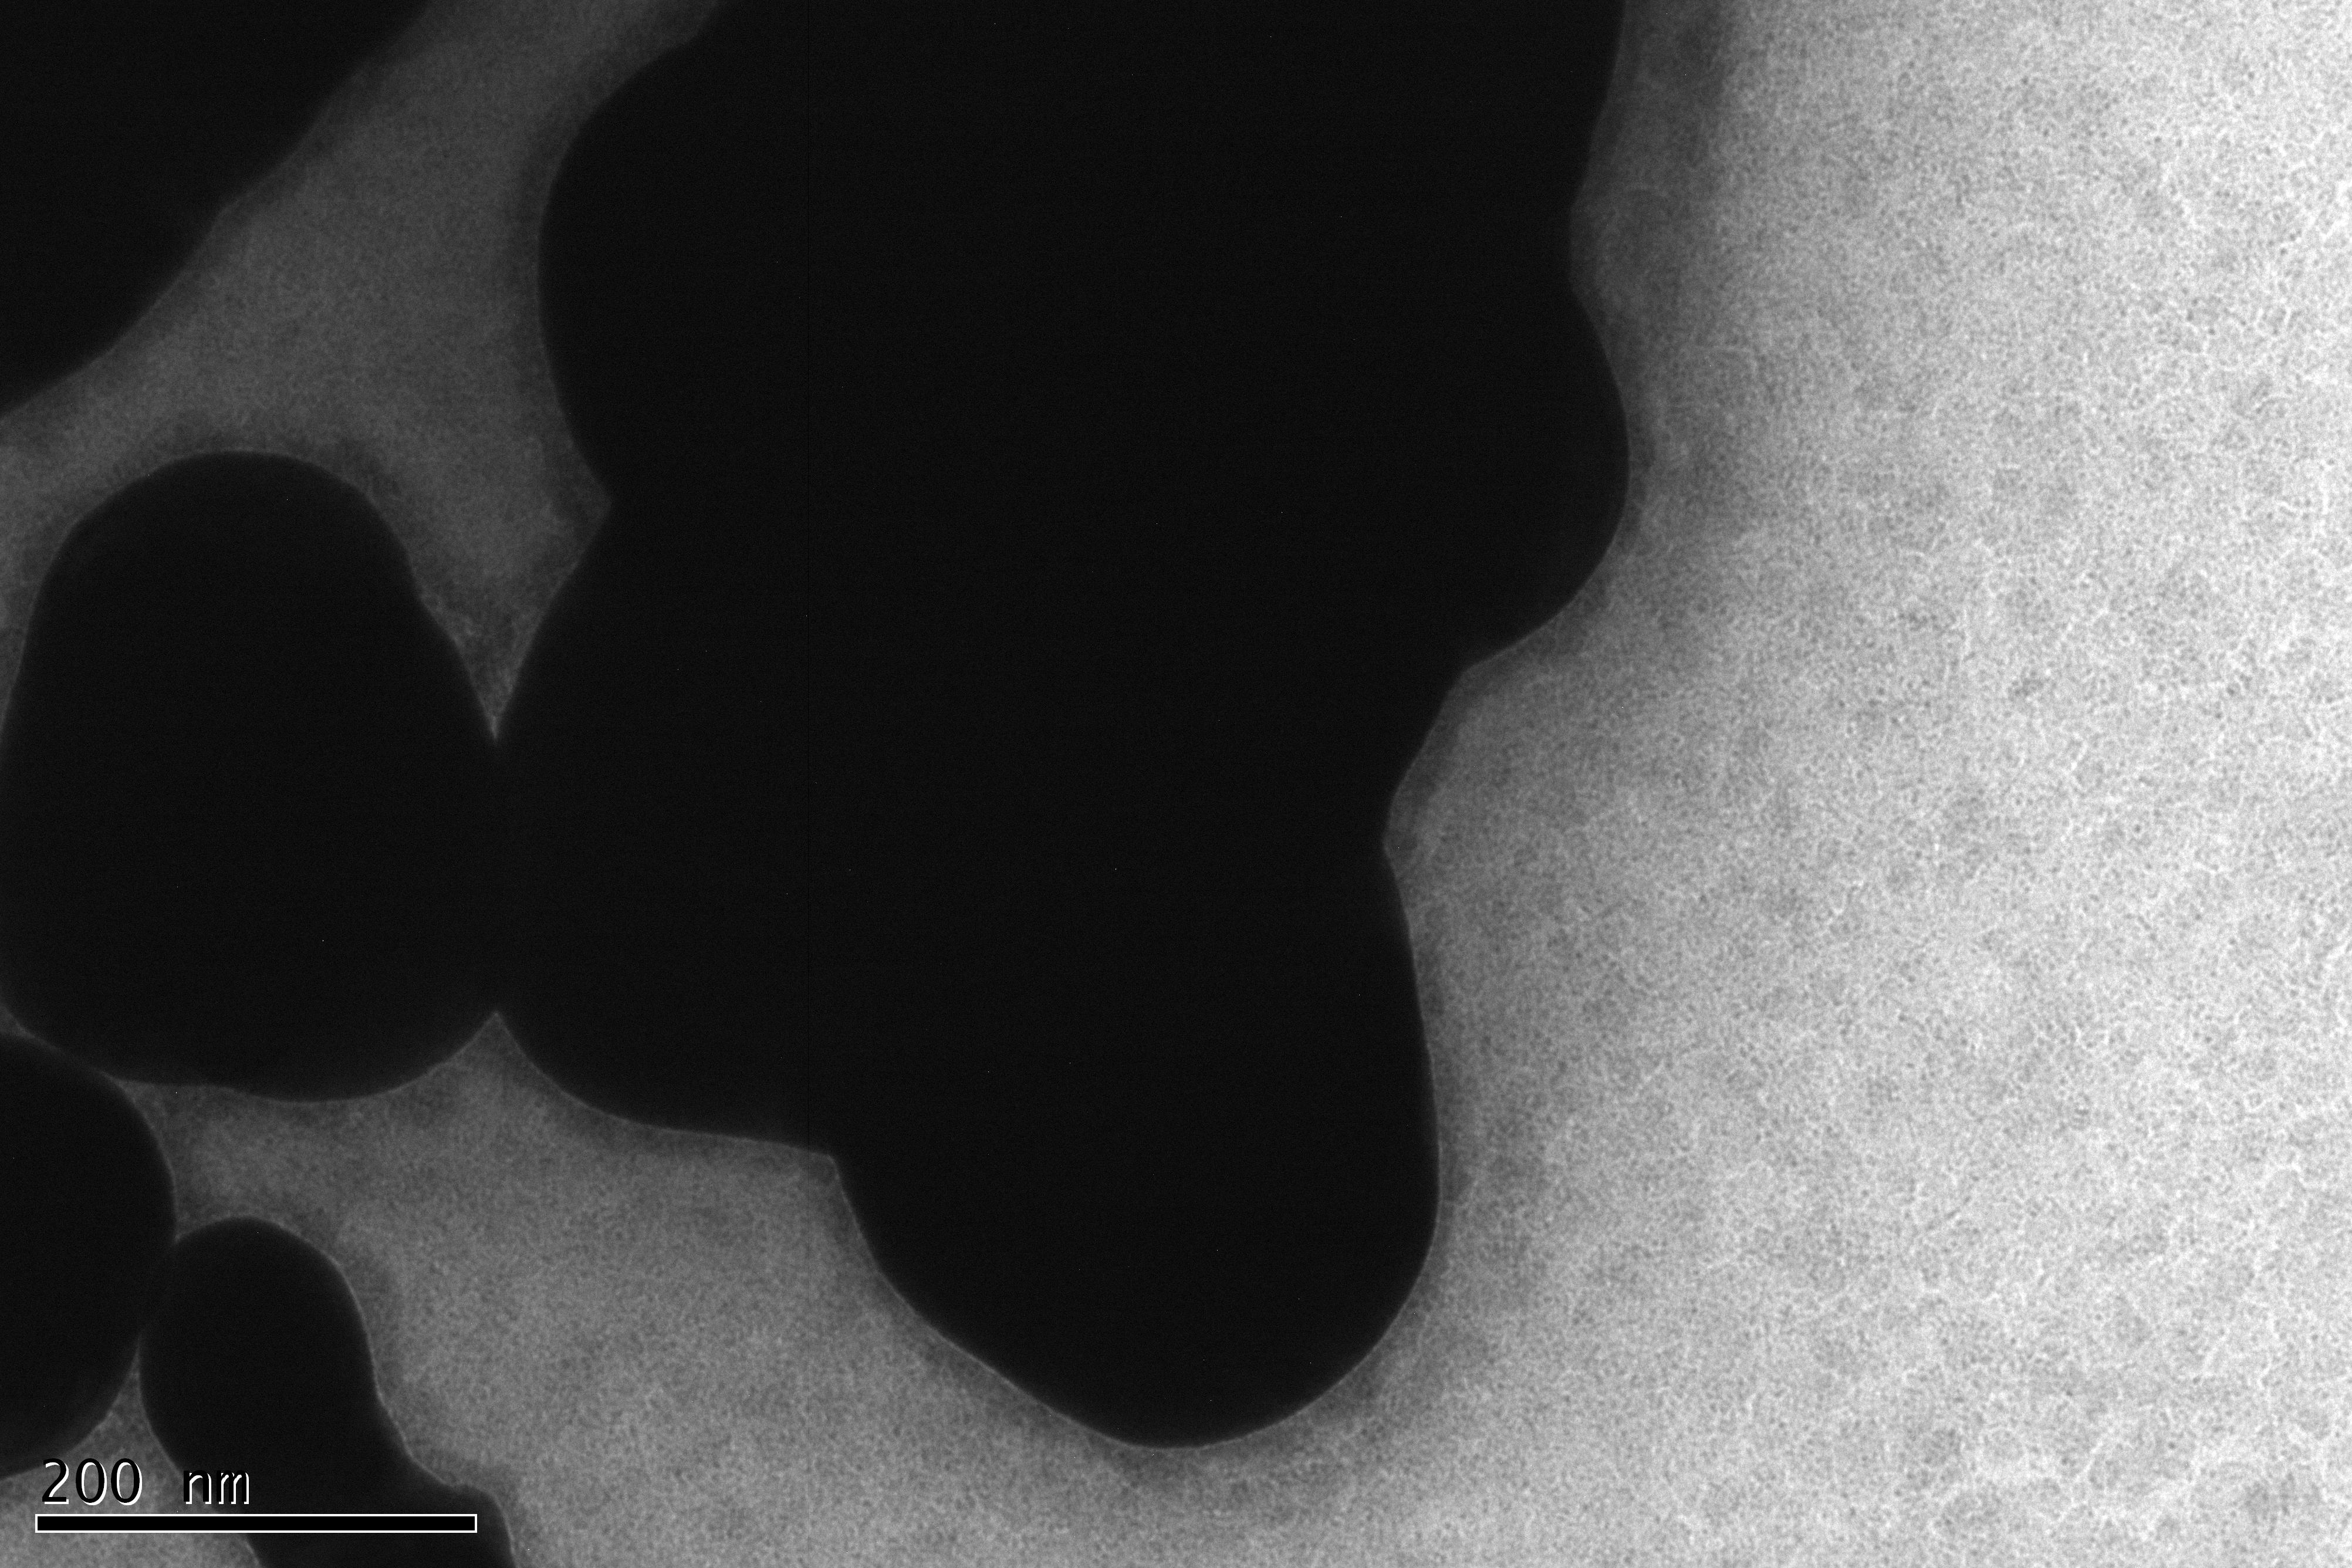
\includegraphics[width=0.33\linewidth]{Bilder/Gel-E-ZnCl-1-10_2}}
			\subfloat[\label{fig:Gel-E-ZnCl-1-10_3}]{%
				\includegraphics[width=0.33\linewidth]{Bilder/Gel-E-ZnCl-1-10_3}}
			\caption{TEM-Aufnahmen des Gels, das mit \ch{Zn[DDTC]2} und \ch{ZnCl2} im Verhältnis 1:10 \ch{Zn[DDTC]2} zu \ch{ZnCl2} behandelt wurde.}
			\label{fig:Gel-E-ZnCl-1-10}
		\end{figure}
	
		Dieser Effekt konnte allerdings bei der Probe mit dem Verhätnis 1:4 nicht beobachtet werden.
		Hier konnte weder das Bilden einer Schale noch das heranwachsen einzelner Partikel am Gel beobachtet werden, wie in \cref{fig:Gel-E-ZnCl-1-4} gezeigt ist.
		
		\begin{figure}[H]
			\centering
			\includegraphics[width=0.6\textwidth]{Bilder/Gel-E-ZnCl-1-4} 	
			\caption{TEM-Aufnahme des Gels, das mit \ch{Zn[DDTC]2} und \ch{ZnCl2} im Verhältnis 1:4 \ch{Zn[DDTC]2} zu \ch{ZnCl2} behandelt wurde.}
			\label{fig:Gel-E-ZnCl-1-4}
		\end{figure}
	
		\subsubsection{Variation der Konzentration}
		Da bei den Versuchen häufig ein Großteil der gebildeten Partikel neben den Gelen vorlag, wurden Reaktionen mit Lösungen mit geringeren Konzentrationen an \ch{Cd[DDTC]2} und \ch{CdCl2} untersucht.
		Bei der Probe mit 0,05~M \ch{Cd[DDTC]2}-Lösung, deren TEM-Messung in \cref{fig:Gel-E-CdS-0,05} dargestellt ist,  zeigt sich ein ähnliches Bild wie bei den Proben mit 0,11~M.
		Es bilden sich viele Partikel , die sich um das Gel herum anlagern, allerdings ist auch hier die Menge an CdS Partikel, die neben dem Gel liegen hoch.
		Eine deutlichere Änderung lässt sich bei der Probe mit 0,01~M \ch{Cd[DDTC]2}-Lösung beobachten, wie \cref{fig:Gel-E-CdS-0,01} zeigt.
		Hier konnten keine CdS-Partikel gefunden werden, die neben dem Gel vorlagen.
		An den Gelen selbst ist eine kleine Schicht CdS zu erkennen.
		Durch die Konzentrationsänderung konnte das Nukleationsverhalten also so angepasst werden, dass sich das CdS am Gel gebildet hat.
		
		\begin{figure}[H]
			\centering
			\includegraphics[width=0.6\textwidth]{Bilder/Gel-E-CdS-0,05} 	
			\caption{TEM-Aufnahme des Gels, das mit 0,05M \ch{Cd[DDTC]2}-Lösung behandelt wurde.}
			\label{fig:Gel-E-CdS-0,05}
		\end{figure}
	
		\begin{figure}[H]
			\centering
			\includegraphics[width=0.6\textwidth]{Bilder/Gel-E-CdS-0,01} 	
			\caption{TEM-Aufnahme des Gels, das mit 0,01M \ch{Cd[DDTC]2}-Lösung behandelt wurde.}
			\label{fig:Gel-E-CdS-0,01}
		\end{figure}
		
		Es wurde auch nochmal der Einfluss von  0,05~M \ch{CdCl2}-Lösung mit einer  0,05~M \ch{Cd[DDTC]2}-Lösung untersucht.
		Hierbei zeigte sich ein ähnliches Bild wie bei den untersuchten Gelen die mit 0,11~M-Lösungen behandelt wurden.
		Sowohl beim  \ch{Cd[DDTC]2}:\ch{CdCl2} Verhältnis 1:1 (\cref{fig:Gel-E-CdCl-1-1-0,05}) als auch 1:4 (\cref{fig:Gel-E-CdCl-1-4-0,05}) als auch 1:10 (\cref{fig:Gel-E-CdCl-1-10-0,05}), konnte die Bildung von CdS beobachtet werden.
		Dieses liegt sowohl zu einem Großteil wieder neben den Gelen vor, wie auch schon bei den vorherigen Proben mit gleichen Verhältnissen mit 0,11~M-Lösungen.
		
		\begin{figure}[H]
			\centering
			\includegraphics[width=0.6\textwidth]{Bilder/Gel-E-CdCl-1-1-0,05} 	
			\caption{TEM-Aufnahme des Gels, das mit \ch{Cd[DDTC]2} und \ch{CdCl2} im Verhältnis 1:1 \ch{Cd[DDTC]2} zu \ch{CdCl2} mit einer Konzentration von 0,05~M behandelt wurde.}
			\label{fig:Gel-E-CdCl-1-1-0,05}
		\end{figure}
		
		\begin{figure}[H]
			\centering
			\includegraphics[width=0.6\textwidth]{Bilder/Gel-E-CdCl-1-4-0,05} 	
			\caption{TEM-Aufnahme des Gels, das mit \ch{Cd[DDTC]2} und \ch{CdCl2} im Verhältnis 1:4 \ch{Cd[DDTC]2} zu \ch{CdCl2} mit einer Konzentration von 0,05~M behandelt wurde.}
			\label{fig:Gel-E-CdCl-1-4-0,05}
		\end{figure}
	
		\begin{figure}[H]
			\centering
			\includegraphics[width=0.6\textwidth]{Bilder/Gel-E-CdCl-1-10-0,05} 	
			\caption{TEM-Aufnahme des Gels, das mit \ch{Cd[DDTC]2} und \ch{CdCl2} im Verhältnis 1:10 \ch{Cd[DDTC]2} zu \ch{CdCl2} mit einer Konzentration von 0,05~M behandelt wurde.}
			\label{fig:Gel-E-CdCl-1-10-0,05}
		\end{figure}
		
	\subsubsection{Variation des Gels}
		Bislang wurden alle Experimente an gleichen Gelen vorgenommen.
		Aus diesem Grund wurden einige Proben mit den Bi-metallischen Au/Ag-Gelen durchgeführt.
		Beim Stufenweisen Austausch der flüssigen Phase der Gele schrumften diese merklich, wie in \cref{fig:Foto-Gel-cit} gezeigt ist.
		Auf dem Foto ist das Gel nach dem Austausch zu sehen. 
		Da kleine Teile des Gels sich am Rand des Gefäßes anhafteten,  kann man daran die Größe der Gele vor dem Austausch gut erkennen. 
		Das resultierende Volumen des Gels nach dem Austausch war etwa ein Drittel vom Ausgangsvolumen.
		Teile der Poren scheinen also während des Austausches der flüssigen Phase kollabiert zu sein.
		
		\begin{figure}[H]
			\centering
			\includegraphics[width=0.6\textwidth]{Bilder/Foto-Gel-cit} 	
			\caption{Bild vom bi-metallischen Au/Ag-Gel nach dem Austausch der flüssigen Phase.}
			\label{fig:Foto-Gel-cit}
		\end{figure}
	
		Die Probe mit dem bi-metallischen Au/Ag-Gel zeigt nach Behandlung mit der 0,11~M \ch{Cd[DDTC]2}-Lösung ein ähnliches Bild wie die vorher verwendeten Gele, wie in \cref{fig:Gel-C-CdS} gezeigt.
		Auch hier bildet sich wieder ein Teil des CdS neben dem Gel.
		Es ist jedoch auch eine kleine Schicht an den Gelen zu erkennen, was in \cref{fig:Gel-C-CdS_2} deutlich zu sehen ist.
		Es konnte also auch an diesem Gel nachträglich CdS herangewachsen werden.
		
		\begin{figure}[htbp]
			\centering
			\subfloat[\label{fig:Gel-C-CdS_1}]{%
				\includegraphics[width=0.45\linewidth]{Bilder/Gel-C-CdS_1}}
			\subfloat[\label{fig:Gel-C-CdS_2}]{%
				\includegraphics[width=0.45\linewidth]{Bilder/Gel-C-CdS_2}}
			\caption{TEM-Bilder des bi-metallischen Au/Ag-Gel nach Behandlung mit 0,11~M \ch{Cd[DDTC]2}-Lösung.}
			\label{fig:Gel-C-CdS}
		\end{figure}
		
		 
		
		
		
		
	   
	
 
 
\pagebreak
% !TEX root = Bigall.tex
\section{Zusammenfassung}
\pagebreak
\printbibliography
\pagebreak
\section{Anhang}
\listoffigures
\pagebreak
\listoftables
%-------------------
\pagebreak
\pagestyle{plain}
\section*{Danksagung}

Die vorliegende Masterarbeit entstand im Arbeitskreis von Prof. Dr. Nadja Bigall am Institut für Physikalische Chemie und Elektrochemie der Leibniz Universität Hannover. Ich möchte mich an dieser Stelle bei allen bedanken, die mich während dieser Arbeit sowohl fachlich als auch moralisch unterstützt haben. Mein besonderer Dank gilt
dabei vor allem:

\begin{itemize}
	\item \textbf{Frau Prof. Dr. Nadja Bigall} für die Möglichkeit diese Arbeit in ihrem Arbeitskreis zu verfassen und ihre stetige Bereitschaft für produktive und interessante Hinweise.
	\item \textbf{Herrn Prof. Dr. Peter Behrens} dafür, dass er als Zweitprüfer zur Verfüngung stand.
	\item \textbf{Pascal Rusch} für seine stets hilfsbereite Art und die TEM-Messungen.
	\item Dem gesamten Arbeitskreis Bigall für das tolle Arbeitsklima.
	\item Meiner Familie und meinen Freunden die immer für mich da sind.
	
\end{itemize}

\pagebreak

\section*{Eidesstattliche Erklärung}

Hiermit versichere ich, die vorliegende Masterarbeit selbstständig, ohne
fremde Hilfe und ohne Benutzung anderer als der von mir angegebenen Quellen
angefertigt zu haben. Alle aus fremden Quellen direkt oder indirekt übernommenen
Gedanken sind als solche gekennzeichnet. Die Arbeit wurde noch
keiner Prüfungsbehörde in gleicher oder ähnlicher Form vorgelegt.

\vspace{5cm}

\noindent Hannover, den 31. März 2020
\vspace{2cm}
\hrule
\vspace{5mm}
\noindent Björn Gastmann
\end{document}